%filename Rapport-asclepiade
% ltex: language=fr
\documentclass{bio}
\author{Harout CHOULGIAN, Akira LAFOREST et Nicolas LANDUCCI}
\title{TODO\\TODO}
\teacher{Louis-Philippe Précourt}
\course{BIO-N02}
\group{2}
\department{Biologie}
\date{4 novembre 2025}

\addbibresource{monarques.bib}

\newcommand{\resize}[1]{\resizebox{\textwidth}{!}{#1}}

\begin{document}
\maketitle
\tocpage


\section{Introduction}
    Bonjour~\parencite{gbif.orgGBIFOccurrenceDownload2025}


    \begin{figure}[H]
        \centering
        \caption{Occurrences d'\textit{Asclepias syriaca} et de \textit{Danaus plexippus} à Montréal depuis 2020}
        \resize{%
            % Created by tikzDevice version 0.12.6 on 2025-10-11 22:32:44
% !TEX encoding = UTF-8 Unicode
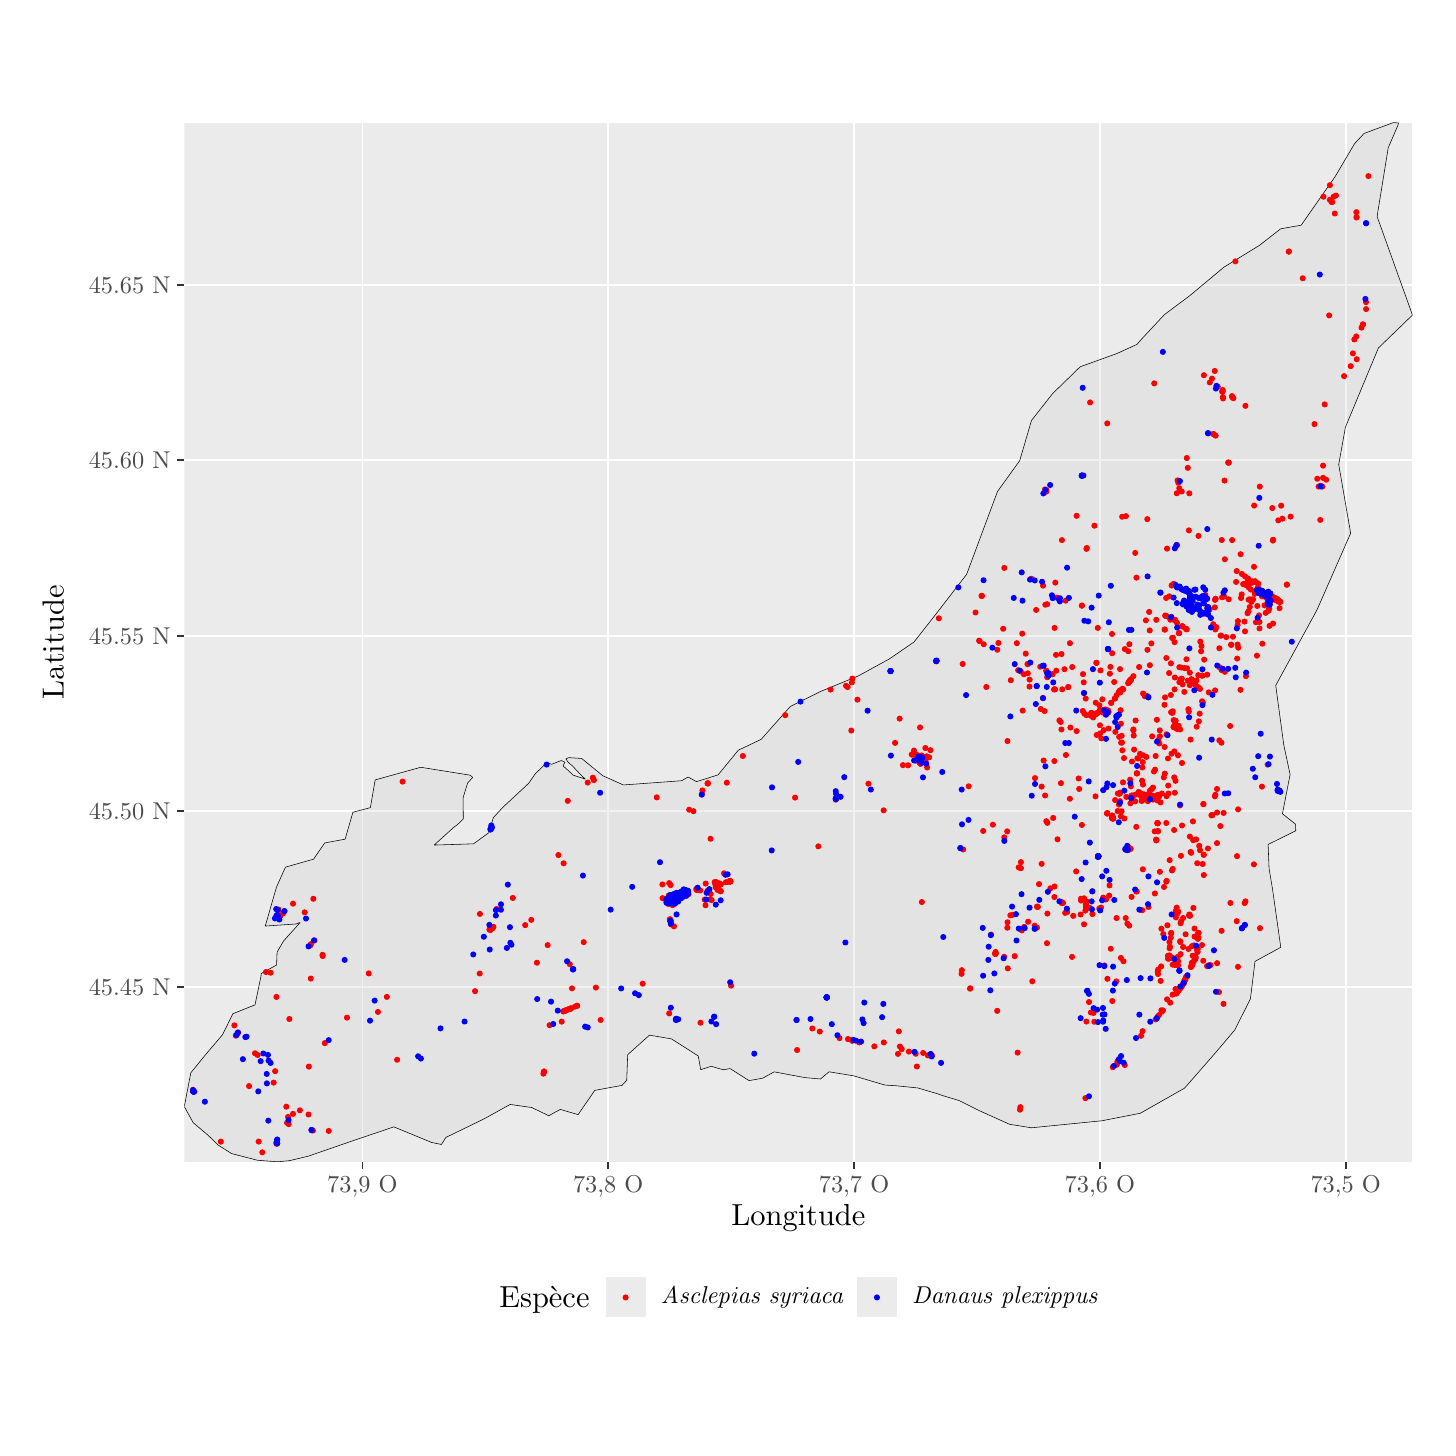
\begin{tikzpicture}[x=1pt,y=1pt]
\definecolor{fillColor}{RGB}{255,255,255}
\path[use as bounding box,fill=fillColor,fill opacity=0.00] (0,0) rectangle (505.89,505.89);
\begin{scope}
\path[clip] (  0.00, 28.82) rectangle (505.89,477.07);
\definecolor{drawColor}{RGB}{255,255,255}
\definecolor{fillColor}{RGB}{255,255,255}

\path[draw=drawColor,line width= 0.6pt,line join=round,line cap=round,fill=fillColor] (  0.00, 28.82) rectangle (505.89,477.07);
\end{scope}
\begin{scope}
\path[clip] ( 56.60, 96.08) rectangle (500.39,471.57);
\definecolor{fillColor}{gray}{0.92}

\path[fill=fillColor] ( 56.60, 96.08) rectangle (500.39,471.57);
\definecolor{drawColor}{RGB}{255,255,255}

\path[draw=drawColor,line width= 0.6pt,line join=round,line cap=round] (120.96, 96.08) --
	(120.96, 99.75) --
	(120.96,103.59) --
	(120.96,107.44) --
	(120.96,111.28) --
	(120.96,115.12) --
	(120.96,118.97) --
	(120.96,122.81) --
	(120.96,126.65) --
	(120.96,130.50) --
	(120.96,134.34) --
	(120.96,138.18) --
	(120.96,142.03) --
	(120.96,145.87) --
	(120.96,149.72) --
	(120.96,153.56) --
	(120.96,157.40) --
	(120.96,161.25) --
	(120.96,165.09) --
	(120.96,168.93) --
	(120.96,172.78) --
	(120.96,176.62) --
	(120.96,180.46) --
	(120.96,184.31) --
	(120.96,188.15) --
	(120.96,191.99) --
	(120.96,195.84) --
	(120.96,199.68) --
	(120.96,203.52) --
	(120.96,207.37) --
	(120.96,211.21) --
	(120.96,215.06) --
	(120.96,218.90) --
	(120.96,222.74) --
	(120.96,226.59) --
	(120.96,230.43) --
	(120.96,234.27) --
	(120.96,238.12) --
	(120.96,241.96) --
	(120.96,245.80) --
	(120.96,249.65) --
	(120.96,253.49) --
	(120.96,257.33) --
	(120.96,261.18) --
	(120.96,265.02) --
	(120.96,268.87) --
	(120.96,272.71) --
	(120.96,276.55) --
	(120.96,280.40) --
	(120.96,284.24) --
	(120.96,288.08) --
	(120.96,291.93) --
	(120.96,295.77) --
	(120.96,299.61) --
	(120.96,303.46) --
	(120.96,307.30) --
	(120.96,311.14) --
	(120.96,314.99) --
	(120.96,318.83) --
	(120.96,322.68) --
	(120.96,326.52) --
	(120.96,330.36) --
	(120.96,334.21) --
	(120.96,338.05) --
	(120.96,341.89) --
	(120.96,345.74) --
	(120.96,349.58) --
	(120.96,353.42) --
	(120.96,357.27) --
	(120.96,361.11) --
	(120.96,364.95) --
	(120.96,368.80) --
	(120.96,372.64) --
	(120.96,376.48) --
	(120.96,380.33) --
	(120.96,384.17) --
	(120.96,388.02) --
	(120.96,391.86) --
	(120.96,395.70) --
	(120.96,399.55) --
	(120.96,403.39) --
	(120.96,407.23) --
	(120.96,411.08) --
	(120.96,414.92) --
	(120.96,418.76) --
	(120.96,422.61) --
	(120.96,426.45) --
	(120.96,430.29) --
	(120.96,434.14) --
	(120.96,437.98) --
	(120.96,441.83) --
	(120.96,445.67) --
	(120.96,449.51) --
	(120.96,453.36) --
	(120.96,457.20) --
	(120.96,461.04) --
	(120.96,464.89) --
	(120.96,468.73) --
	(120.96,471.57);

\path[draw=drawColor,line width= 0.6pt,line join=round,line cap=round] (209.79, 96.08) --
	(209.79, 99.75) --
	(209.79,103.59) --
	(209.79,107.44) --
	(209.79,111.28) --
	(209.79,115.12) --
	(209.79,118.97) --
	(209.79,122.81) --
	(209.79,126.65) --
	(209.79,130.50) --
	(209.79,134.34) --
	(209.79,138.18) --
	(209.79,142.03) --
	(209.79,145.87) --
	(209.79,149.72) --
	(209.79,153.56) --
	(209.79,157.40) --
	(209.79,161.25) --
	(209.79,165.09) --
	(209.79,168.93) --
	(209.79,172.78) --
	(209.79,176.62) --
	(209.79,180.46) --
	(209.79,184.31) --
	(209.79,188.15) --
	(209.79,191.99) --
	(209.79,195.84) --
	(209.79,199.68) --
	(209.79,203.52) --
	(209.79,207.37) --
	(209.79,211.21) --
	(209.79,215.06) --
	(209.79,218.90) --
	(209.79,222.74) --
	(209.79,226.59) --
	(209.79,230.43) --
	(209.79,234.27) --
	(209.79,238.12) --
	(209.79,241.96) --
	(209.79,245.80) --
	(209.79,249.65) --
	(209.79,253.49) --
	(209.79,257.33) --
	(209.79,261.18) --
	(209.79,265.02) --
	(209.79,268.87) --
	(209.79,272.71) --
	(209.79,276.55) --
	(209.79,280.40) --
	(209.79,284.24) --
	(209.79,288.08) --
	(209.79,291.93) --
	(209.79,295.77) --
	(209.79,299.61) --
	(209.79,303.46) --
	(209.79,307.30) --
	(209.79,311.14) --
	(209.79,314.99) --
	(209.79,318.83) --
	(209.79,322.68) --
	(209.79,326.52) --
	(209.79,330.36) --
	(209.79,334.21) --
	(209.79,338.05) --
	(209.79,341.89) --
	(209.79,345.74) --
	(209.79,349.58) --
	(209.79,353.42) --
	(209.79,357.27) --
	(209.79,361.11) --
	(209.79,364.95) --
	(209.79,368.80) --
	(209.79,372.64) --
	(209.79,376.48) --
	(209.79,380.33) --
	(209.79,384.17) --
	(209.79,388.02) --
	(209.79,391.86) --
	(209.79,395.70) --
	(209.79,399.55) --
	(209.79,403.39) --
	(209.79,407.23) --
	(209.79,411.08) --
	(209.79,414.92) --
	(209.79,418.76) --
	(209.79,422.61) --
	(209.79,426.45) --
	(209.79,430.29) --
	(209.79,434.14) --
	(209.79,437.98) --
	(209.79,441.83) --
	(209.79,445.67) --
	(209.79,449.51) --
	(209.79,453.36) --
	(209.79,457.20) --
	(209.79,461.04) --
	(209.79,464.89) --
	(209.79,468.73) --
	(209.79,471.57);

\path[draw=drawColor,line width= 0.6pt,line join=round,line cap=round] (298.61, 96.08) --
	(298.61, 99.75) --
	(298.61,103.59) --
	(298.61,107.44) --
	(298.61,111.28) --
	(298.61,115.12) --
	(298.61,118.97) --
	(298.61,122.81) --
	(298.61,126.65) --
	(298.61,130.50) --
	(298.61,134.34) --
	(298.61,138.18) --
	(298.61,142.03) --
	(298.61,145.87) --
	(298.61,149.72) --
	(298.61,153.56) --
	(298.61,157.40) --
	(298.61,161.25) --
	(298.61,165.09) --
	(298.61,168.93) --
	(298.61,172.78) --
	(298.61,176.62) --
	(298.61,180.46) --
	(298.61,184.31) --
	(298.61,188.15) --
	(298.61,191.99) --
	(298.61,195.84) --
	(298.61,199.68) --
	(298.61,203.52) --
	(298.61,207.37) --
	(298.61,211.21) --
	(298.61,215.06) --
	(298.61,218.90) --
	(298.61,222.74) --
	(298.61,226.59) --
	(298.61,230.43) --
	(298.61,234.27) --
	(298.61,238.12) --
	(298.61,241.96) --
	(298.61,245.80) --
	(298.61,249.65) --
	(298.61,253.49) --
	(298.61,257.33) --
	(298.61,261.18) --
	(298.61,265.02) --
	(298.61,268.87) --
	(298.61,272.71) --
	(298.61,276.55) --
	(298.61,280.40) --
	(298.61,284.24) --
	(298.61,288.08) --
	(298.61,291.93) --
	(298.61,295.77) --
	(298.61,299.61) --
	(298.61,303.46) --
	(298.61,307.30) --
	(298.61,311.14) --
	(298.61,314.99) --
	(298.61,318.83) --
	(298.61,322.68) --
	(298.61,326.52) --
	(298.61,330.36) --
	(298.61,334.21) --
	(298.61,338.05) --
	(298.61,341.89) --
	(298.61,345.74) --
	(298.61,349.58) --
	(298.61,353.42) --
	(298.61,357.27) --
	(298.61,361.11) --
	(298.61,364.95) --
	(298.61,368.80) --
	(298.61,372.64) --
	(298.61,376.48) --
	(298.61,380.33) --
	(298.61,384.17) --
	(298.61,388.02) --
	(298.61,391.86) --
	(298.61,395.70) --
	(298.61,399.55) --
	(298.61,403.39) --
	(298.61,407.23) --
	(298.61,411.08) --
	(298.61,414.92) --
	(298.61,418.76) --
	(298.61,422.61) --
	(298.61,426.45) --
	(298.61,430.29) --
	(298.61,434.14) --
	(298.61,437.98) --
	(298.61,441.83) --
	(298.61,445.67) --
	(298.61,449.51) --
	(298.61,453.36) --
	(298.61,457.20) --
	(298.61,461.04) --
	(298.61,464.89) --
	(298.61,468.73) --
	(298.61,471.57);

\path[draw=drawColor,line width= 0.6pt,line join=round,line cap=round] (387.44, 96.08) --
	(387.44, 99.75) --
	(387.44,103.59) --
	(387.44,107.44) --
	(387.44,111.28) --
	(387.44,115.12) --
	(387.44,118.97) --
	(387.44,122.81) --
	(387.44,126.65) --
	(387.44,130.50) --
	(387.44,134.34) --
	(387.44,138.18) --
	(387.44,142.03) --
	(387.44,145.87) --
	(387.44,149.72) --
	(387.44,153.56) --
	(387.44,157.40) --
	(387.44,161.25) --
	(387.44,165.09) --
	(387.44,168.93) --
	(387.44,172.78) --
	(387.44,176.62) --
	(387.44,180.46) --
	(387.44,184.31) --
	(387.44,188.15) --
	(387.44,191.99) --
	(387.44,195.84) --
	(387.44,199.68) --
	(387.44,203.52) --
	(387.44,207.37) --
	(387.44,211.21) --
	(387.44,215.06) --
	(387.44,218.90) --
	(387.44,222.74) --
	(387.44,226.59) --
	(387.44,230.43) --
	(387.44,234.27) --
	(387.44,238.12) --
	(387.44,241.96) --
	(387.44,245.80) --
	(387.44,249.65) --
	(387.44,253.49) --
	(387.44,257.33) --
	(387.44,261.18) --
	(387.44,265.02) --
	(387.44,268.87) --
	(387.44,272.71) --
	(387.44,276.55) --
	(387.44,280.40) --
	(387.44,284.24) --
	(387.44,288.08) --
	(387.44,291.93) --
	(387.44,295.77) --
	(387.44,299.61) --
	(387.44,303.46) --
	(387.44,307.30) --
	(387.44,311.14) --
	(387.44,314.99) --
	(387.44,318.83) --
	(387.44,322.68) --
	(387.44,326.52) --
	(387.44,330.36) --
	(387.44,334.21) --
	(387.44,338.05) --
	(387.44,341.89) --
	(387.44,345.74) --
	(387.44,349.58) --
	(387.44,353.42) --
	(387.44,357.27) --
	(387.44,361.11) --
	(387.44,364.95) --
	(387.44,368.80) --
	(387.44,372.64) --
	(387.44,376.48) --
	(387.44,380.33) --
	(387.44,384.17) --
	(387.44,388.02) --
	(387.44,391.86) --
	(387.44,395.70) --
	(387.44,399.55) --
	(387.44,403.39) --
	(387.44,407.23) --
	(387.44,411.08) --
	(387.44,414.92) --
	(387.44,418.76) --
	(387.44,422.61) --
	(387.44,426.45) --
	(387.44,430.29) --
	(387.44,434.14) --
	(387.44,437.98) --
	(387.44,441.83) --
	(387.44,445.67) --
	(387.44,449.51) --
	(387.44,453.36) --
	(387.44,457.20) --
	(387.44,461.04) --
	(387.44,464.89) --
	(387.44,468.73) --
	(387.44,471.57);

\path[draw=drawColor,line width= 0.6pt,line join=round,line cap=round] (476.26, 96.08) --
	(476.26, 99.75) --
	(476.26,103.59) --
	(476.26,107.44) --
	(476.26,111.28) --
	(476.26,115.12) --
	(476.26,118.97) --
	(476.26,122.81) --
	(476.26,126.65) --
	(476.26,130.50) --
	(476.26,134.34) --
	(476.26,138.18) --
	(476.26,142.03) --
	(476.26,145.87) --
	(476.26,149.72) --
	(476.26,153.56) --
	(476.26,157.40) --
	(476.26,161.25) --
	(476.26,165.09) --
	(476.26,168.93) --
	(476.26,172.78) --
	(476.26,176.62) --
	(476.26,180.46) --
	(476.26,184.31) --
	(476.26,188.15) --
	(476.26,191.99) --
	(476.26,195.84) --
	(476.26,199.68) --
	(476.26,203.52) --
	(476.26,207.37) --
	(476.26,211.21) --
	(476.26,215.06) --
	(476.26,218.90) --
	(476.26,222.74) --
	(476.26,226.59) --
	(476.26,230.43) --
	(476.26,234.27) --
	(476.26,238.12) --
	(476.26,241.96) --
	(476.26,245.80) --
	(476.26,249.65) --
	(476.26,253.49) --
	(476.26,257.33) --
	(476.26,261.18) --
	(476.26,265.02) --
	(476.26,268.87) --
	(476.26,272.71) --
	(476.26,276.55) --
	(476.26,280.40) --
	(476.26,284.24) --
	(476.26,288.08) --
	(476.26,291.93) --
	(476.26,295.77) --
	(476.26,299.61) --
	(476.26,303.46) --
	(476.26,307.30) --
	(476.26,311.14) --
	(476.26,314.99) --
	(476.26,318.83) --
	(476.26,322.68) --
	(476.26,326.52) --
	(476.26,330.36) --
	(476.26,334.21) --
	(476.26,338.05) --
	(476.26,341.89) --
	(476.26,345.74) --
	(476.26,349.58) --
	(476.26,353.42) --
	(476.26,357.27) --
	(476.26,361.11) --
	(476.26,364.95) --
	(476.26,368.80) --
	(476.26,372.64) --
	(476.26,376.48) --
	(476.26,380.33) --
	(476.26,384.17) --
	(476.26,388.02) --
	(476.26,391.86) --
	(476.26,395.70) --
	(476.26,399.55) --
	(476.26,403.39) --
	(476.26,407.23) --
	(476.26,411.08) --
	(476.26,414.92) --
	(476.26,418.76) --
	(476.26,422.61) --
	(476.26,426.45) --
	(476.26,430.29) --
	(476.26,434.14) --
	(476.26,437.98) --
	(476.26,441.83) --
	(476.26,445.67) --
	(476.26,449.51) --
	(476.26,453.36) --
	(476.26,457.20) --
	(476.26,461.04) --
	(476.26,464.89) --
	(476.26,468.73) --
	(476.26,471.57);

\path[draw=drawColor,line width= 0.6pt,line join=round,line cap=round] ( 56.60,159.32) --
	( 59.05,159.32) --
	( 64.44,159.32) --
	( 69.82,159.32) --
	( 75.20,159.32) --
	( 80.59,159.32) --
	( 85.97,159.32) --
	( 91.35,159.32) --
	( 96.74,159.32) --
	(102.12,159.32) --
	(107.50,159.32) --
	(112.89,159.32) --
	(118.27,159.32) --
	(123.65,159.32) --
	(129.04,159.32) --
	(134.42,159.32) --
	(139.80,159.32) --
	(145.19,159.32) --
	(150.57,159.32) --
	(155.95,159.32) --
	(161.34,159.32) --
	(166.72,159.32) --
	(172.10,159.32) --
	(177.49,159.32) --
	(182.87,159.32) --
	(188.25,159.32) --
	(193.64,159.32) --
	(199.02,159.32) --
	(204.40,159.32) --
	(209.79,159.32) --
	(215.17,159.32) --
	(220.55,159.32) --
	(225.94,159.32) --
	(231.32,159.32) --
	(236.70,159.32) --
	(242.09,159.32) --
	(247.47,159.32) --
	(252.85,159.32) --
	(258.24,159.32) --
	(263.62,159.32) --
	(269.00,159.32) --
	(274.39,159.32) --
	(279.77,159.32) --
	(285.15,159.32) --
	(290.54,159.32) --
	(295.92,159.32) --
	(301.31,159.32) --
	(306.69,159.32) --
	(312.07,159.32) --
	(317.46,159.32) --
	(322.84,159.32) --
	(328.22,159.32) --
	(333.61,159.32) --
	(338.99,159.32) --
	(344.37,159.32) --
	(349.76,159.32) --
	(355.14,159.32) --
	(360.52,159.32) --
	(365.91,159.32) --
	(371.29,159.32) --
	(376.67,159.32) --
	(382.06,159.32) --
	(387.44,159.32) --
	(392.82,159.32) --
	(398.21,159.32) --
	(403.59,159.32) --
	(408.97,159.32) --
	(414.36,159.32) --
	(419.74,159.32) --
	(425.12,159.32) --
	(430.51,159.32) --
	(435.89,159.32) --
	(441.27,159.32) --
	(446.66,159.32) --
	(452.04,159.32) --
	(457.42,159.32) --
	(462.81,159.32) --
	(468.19,159.32) --
	(473.57,159.32) --
	(478.96,159.32) --
	(484.34,159.32) --
	(489.72,159.32) --
	(495.11,159.32) --
	(500.39,159.32);

\path[draw=drawColor,line width= 0.6pt,line join=round,line cap=round] ( 56.60,222.74) --
	( 59.05,222.74) --
	( 64.44,222.74) --
	( 69.82,222.74) --
	( 75.20,222.74) --
	( 80.59,222.74) --
	( 85.97,222.74) --
	( 91.35,222.74) --
	( 96.74,222.74) --
	(102.12,222.74) --
	(107.50,222.74) --
	(112.89,222.74) --
	(118.27,222.74) --
	(123.65,222.74) --
	(129.04,222.74) --
	(134.42,222.74) --
	(139.80,222.74) --
	(145.19,222.74) --
	(150.57,222.74) --
	(155.95,222.74) --
	(161.34,222.74) --
	(166.72,222.74) --
	(172.10,222.74) --
	(177.49,222.74) --
	(182.87,222.74) --
	(188.25,222.74) --
	(193.64,222.74) --
	(199.02,222.74) --
	(204.40,222.74) --
	(209.79,222.74) --
	(215.17,222.74) --
	(220.55,222.74) --
	(225.94,222.74) --
	(231.32,222.74) --
	(236.70,222.74) --
	(242.09,222.74) --
	(247.47,222.74) --
	(252.85,222.74) --
	(258.24,222.74) --
	(263.62,222.74) --
	(269.00,222.74) --
	(274.39,222.74) --
	(279.77,222.74) --
	(285.15,222.74) --
	(290.54,222.74) --
	(295.92,222.74) --
	(301.31,222.74) --
	(306.69,222.74) --
	(312.07,222.74) --
	(317.46,222.74) --
	(322.84,222.74) --
	(328.22,222.74) --
	(333.61,222.74) --
	(338.99,222.74) --
	(344.37,222.74) --
	(349.76,222.74) --
	(355.14,222.74) --
	(360.52,222.74) --
	(365.91,222.74) --
	(371.29,222.74) --
	(376.67,222.74) --
	(382.06,222.74) --
	(387.44,222.74) --
	(392.82,222.74) --
	(398.21,222.74) --
	(403.59,222.74) --
	(408.97,222.74) --
	(414.36,222.74) --
	(419.74,222.74) --
	(425.12,222.74) --
	(430.51,222.74) --
	(435.89,222.74) --
	(441.27,222.74) --
	(446.66,222.74) --
	(452.04,222.74) --
	(457.42,222.74) --
	(462.81,222.74) --
	(468.19,222.74) --
	(473.57,222.74) --
	(478.96,222.74) --
	(484.34,222.74) --
	(489.72,222.74) --
	(495.11,222.74) --
	(500.39,222.74);

\path[draw=drawColor,line width= 0.6pt,line join=round,line cap=round] ( 56.60,286.16) --
	( 59.05,286.16) --
	( 64.44,286.16) --
	( 69.82,286.16) --
	( 75.20,286.16) --
	( 80.59,286.16) --
	( 85.97,286.16) --
	( 91.35,286.16) --
	( 96.74,286.16) --
	(102.12,286.16) --
	(107.50,286.16) --
	(112.89,286.16) --
	(118.27,286.16) --
	(123.65,286.16) --
	(129.04,286.16) --
	(134.42,286.16) --
	(139.80,286.16) --
	(145.19,286.16) --
	(150.57,286.16) --
	(155.95,286.16) --
	(161.34,286.16) --
	(166.72,286.16) --
	(172.10,286.16) --
	(177.49,286.16) --
	(182.87,286.16) --
	(188.25,286.16) --
	(193.64,286.16) --
	(199.02,286.16) --
	(204.40,286.16) --
	(209.79,286.16) --
	(215.17,286.16) --
	(220.55,286.16) --
	(225.94,286.16) --
	(231.32,286.16) --
	(236.70,286.16) --
	(242.09,286.16) --
	(247.47,286.16) --
	(252.85,286.16) --
	(258.24,286.16) --
	(263.62,286.16) --
	(269.00,286.16) --
	(274.39,286.16) --
	(279.77,286.16) --
	(285.15,286.16) --
	(290.54,286.16) --
	(295.92,286.16) --
	(301.31,286.16) --
	(306.69,286.16) --
	(312.07,286.16) --
	(317.46,286.16) --
	(322.84,286.16) --
	(328.22,286.16) --
	(333.61,286.16) --
	(338.99,286.16) --
	(344.37,286.16) --
	(349.76,286.16) --
	(355.14,286.16) --
	(360.52,286.16) --
	(365.91,286.16) --
	(371.29,286.16) --
	(376.67,286.16) --
	(382.06,286.16) --
	(387.44,286.16) --
	(392.82,286.16) --
	(398.21,286.16) --
	(403.59,286.16) --
	(408.97,286.16) --
	(414.36,286.16) --
	(419.74,286.16) --
	(425.12,286.16) --
	(430.51,286.16) --
	(435.89,286.16) --
	(441.27,286.16) --
	(446.66,286.16) --
	(452.04,286.16) --
	(457.42,286.16) --
	(462.81,286.16) --
	(468.19,286.16) --
	(473.57,286.16) --
	(478.96,286.16) --
	(484.34,286.16) --
	(489.72,286.16) --
	(495.11,286.16) --
	(500.39,286.16);

\path[draw=drawColor,line width= 0.6pt,line join=round,line cap=round] ( 56.60,349.58) --
	( 59.05,349.58) --
	( 64.44,349.58) --
	( 69.82,349.58) --
	( 75.20,349.58) --
	( 80.59,349.58) --
	( 85.97,349.58) --
	( 91.35,349.58) --
	( 96.74,349.58) --
	(102.12,349.58) --
	(107.50,349.58) --
	(112.89,349.58) --
	(118.27,349.58) --
	(123.65,349.58) --
	(129.04,349.58) --
	(134.42,349.58) --
	(139.80,349.58) --
	(145.19,349.58) --
	(150.57,349.58) --
	(155.95,349.58) --
	(161.34,349.58) --
	(166.72,349.58) --
	(172.10,349.58) --
	(177.49,349.58) --
	(182.87,349.58) --
	(188.25,349.58) --
	(193.64,349.58) --
	(199.02,349.58) --
	(204.40,349.58) --
	(209.79,349.58) --
	(215.17,349.58) --
	(220.55,349.58) --
	(225.94,349.58) --
	(231.32,349.58) --
	(236.70,349.58) --
	(242.09,349.58) --
	(247.47,349.58) --
	(252.85,349.58) --
	(258.24,349.58) --
	(263.62,349.58) --
	(269.00,349.58) --
	(274.39,349.58) --
	(279.77,349.58) --
	(285.15,349.58) --
	(290.54,349.58) --
	(295.92,349.58) --
	(301.31,349.58) --
	(306.69,349.58) --
	(312.07,349.58) --
	(317.46,349.58) --
	(322.84,349.58) --
	(328.22,349.58) --
	(333.61,349.58) --
	(338.99,349.58) --
	(344.37,349.58) --
	(349.76,349.58) --
	(355.14,349.58) --
	(360.52,349.58) --
	(365.91,349.58) --
	(371.29,349.58) --
	(376.67,349.58) --
	(382.06,349.58) --
	(387.44,349.58) --
	(392.82,349.58) --
	(398.21,349.58) --
	(403.59,349.58) --
	(408.97,349.58) --
	(414.36,349.58) --
	(419.74,349.58) --
	(425.12,349.58) --
	(430.51,349.58) --
	(435.89,349.58) --
	(441.27,349.58) --
	(446.66,349.58) --
	(452.04,349.58) --
	(457.42,349.58) --
	(462.81,349.58) --
	(468.19,349.58) --
	(473.57,349.58) --
	(478.96,349.58) --
	(484.34,349.58) --
	(489.72,349.58) --
	(495.11,349.58) --
	(500.39,349.58);

\path[draw=drawColor,line width= 0.6pt,line join=round,line cap=round] ( 56.60,413.00) --
	( 59.05,413.00) --
	( 64.44,413.00) --
	( 69.82,413.00) --
	( 75.20,413.00) --
	( 80.59,413.00) --
	( 85.97,413.00) --
	( 91.35,413.00) --
	( 96.74,413.00) --
	(102.12,413.00) --
	(107.50,413.00) --
	(112.89,413.00) --
	(118.27,413.00) --
	(123.65,413.00) --
	(129.04,413.00) --
	(134.42,413.00) --
	(139.80,413.00) --
	(145.19,413.00) --
	(150.57,413.00) --
	(155.95,413.00) --
	(161.34,413.00) --
	(166.72,413.00) --
	(172.10,413.00) --
	(177.49,413.00) --
	(182.87,413.00) --
	(188.25,413.00) --
	(193.64,413.00) --
	(199.02,413.00) --
	(204.40,413.00) --
	(209.79,413.00) --
	(215.17,413.00) --
	(220.55,413.00) --
	(225.94,413.00) --
	(231.32,413.00) --
	(236.70,413.00) --
	(242.09,413.00) --
	(247.47,413.00) --
	(252.85,413.00) --
	(258.24,413.00) --
	(263.62,413.00) --
	(269.00,413.00) --
	(274.39,413.00) --
	(279.77,413.00) --
	(285.15,413.00) --
	(290.54,413.00) --
	(295.92,413.00) --
	(301.31,413.00) --
	(306.69,413.00) --
	(312.07,413.00) --
	(317.46,413.00) --
	(322.84,413.00) --
	(328.22,413.00) --
	(333.61,413.00) --
	(338.99,413.00) --
	(344.37,413.00) --
	(349.76,413.00) --
	(355.14,413.00) --
	(360.52,413.00) --
	(365.91,413.00) --
	(371.29,413.00) --
	(376.67,413.00) --
	(382.06,413.00) --
	(387.44,413.00) --
	(392.82,413.00) --
	(398.21,413.00) --
	(403.59,413.00) --
	(408.97,413.00) --
	(414.36,413.00) --
	(419.74,413.00) --
	(425.12,413.00) --
	(430.51,413.00) --
	(435.89,413.00) --
	(441.27,413.00) --
	(446.66,413.00) --
	(452.04,413.00) --
	(457.42,413.00) --
	(462.81,413.00) --
	(468.19,413.00) --
	(473.57,413.00) --
	(478.96,413.00) --
	(484.34,413.00) --
	(489.72,413.00) --
	(495.11,413.00) --
	(500.39,413.00);
\definecolor{drawColor}{RGB}{0,0,0}
\definecolor{fillColor}{RGB}{211,211,211}

\path[draw=drawColor,line width= 0.2pt,line join=round,fill=fillColor,fill opacity=0.30,even odd rule]
	(101.38, 98.10) --
	( 98.88, 97.50) --
	( 97.78, 97.24) --
	( 96.63, 96.97) --
	( 95.12, 96.61) --
	( 94.55, 96.47) --
	( 92.38, 96.27) --
	( 90.71, 96.11) --
	( 90.34, 96.08) --
	( 90.23, 96.09) --
	( 89.25, 96.16) --
	( 85.00, 96.48) --
	( 83.83, 96.57) --
	( 83.09, 96.62) --
	( 73.70, 99.04) --
	( 72.52, 99.78) --
	( 68.74,102.18) --
	( 66.74,104.14) --
	( 66.31,104.57) --
	( 65.20,105.65) --
	( 61.20,109.03) --
	( 59.80,110.22) --
	( 58.71,112.21) --
	( 56.60,116.04) --
	( 56.89,117.54) --
	( 57.52,120.83) --
	( 58.36,125.16) --
	( 58.95,128.23) --
	( 64.34,134.86) --
	( 70.39,141.97) --
	( 71.16,143.54) --
	( 71.38,143.97) --
	( 73.02,147.28) --
	( 74.15,149.58) --
	( 76.25,150.42) --
	( 76.36,150.46) --
	( 76.51,150.52) --
	( 82.15,152.78) --
	( 84.27,162.97) --
	( 84.31,163.35) --
	( 84.41,164.12) --
	( 85.63,164.80) --
	( 87.54,165.86) --
	( 89.02,166.68) --
	( 89.94,167.19) --
	( 89.98,168.26) --
	( 90.07,170.47) --
	( 90.12,171.82) --
	( 92.44,175.83) --
	( 94.21,177.80) --
	( 97.53,181.49) --
	( 98.43,182.48) --
	( 97.87,182.39) --
	( 97.47,182.21) --
	( 97.41,182.18) --
	( 97.05,182.01) --
	( 85.85,181.26) --
	( 88.14,189.21) --
	( 88.28,189.71) --
	( 88.81,191.54) --
	( 89.90,195.30) --
	( 92.19,200.42) --
	( 93.15,202.54) --
	(103.31,205.44) --
	(105.03,207.95) --
	(107.33,211.29) --
	(110.40,211.86) --
	(111.65,212.09) --
	(114.71,212.65) --
	(116.31,218.19) --
	(117.52,222.37) --
	(119.19,222.82) --
	(123.83,224.04) --
	(125.57,234.07) --
	(127.70,234.66) --
	(142.05,238.63) --
	(157.73,236.12) --
	(159.88,235.77) --
	(160.82,234.99) --
	(160.63,234.78) --
	(159.26,233.25) --
	(158.99,232.95) --
	(158.61,231.75) --
	(158.13,230.19) --
	(157.35,227.70) --
	(157.38,223.47) --
	(157.39,221.65) --
	(157.41,220.02) --
	(157.06,219.62) --
	(156.84,219.38) --
	(156.74,219.27) --
	(156.41,218.93) --
	(156.33,218.85) --
	(156.24,218.77) --
	(156.07,218.60) --
	(155.77,218.33) --
	(155.67,218.25) --
	(155.35,217.97) --
	(154.97,217.68) --
	(154.79,217.54) --
	(154.66,217.44) --
	(154.59,217.39) --
	(154.38,217.25) --
	(154.28,217.18) --
	(154.19,217.13) --
	(146.88,210.52) --
	(151.70,210.67) --
	(155.52,210.79) --
	(157.65,210.86) --
	(157.85,210.87) --
	(161.12,210.97) --
	(162.59,212.05) --
	(164.83,213.68) --
	(166.70,215.04) --
	(166.89,215.68) --
	(167.08,216.36) --
	(167.83,218.94) --
	(168.26,220.44) --
	(169.98,222.30) --
	(171.67,224.13) --
	(175.70,227.88) --
	(177.16,229.23) --
	(181.04,232.84) --
	(183.41,236.28) --
	(185.14,237.96) --
	(187.52,240.27) --
	(189.31,239.72) --
	(190.83,240.30) --
	(192.76,241.05) --
	(193.37,240.85) --
	(194.10,240.46) --
	(193.72,239.67) --
	(193.51,239.10) --
	(196.40,236.48) --
	(197.15,235.76) --
	(198.42,235.36) --
	(201.46,234.37) --
	(199.29,236.51) --
	(196.77,239.21) --
	(196.22,239.63) --
	(195.39,240.34) --
	(194.84,241.09) --
	(194.84,241.24) --
	(194.68,241.41) --
	(194.44,241.69) --
	(195.54,242.12) --
	(199.87,241.84) --
	(200.19,241.82) --
	(207.80,235.58) --
	(213.22,233.15) --
	(214.78,232.45) --
	(215.24,232.24) --
	(225.32,232.97) --
	(236.30,233.77) --
	(238.07,234.79) --
	(238.63,235.11) --
	(239.03,234.90) --
	(241.67,233.44) --
	(245.07,234.50) --
	(245.42,234.61) --
	(246.12,234.83) --
	(246.41,234.92) --
	(249.48,235.89) --
	(256.80,244.81) --
	(257.69,245.23) --
	(265.04,248.72) --
	(268.95,253.13) --
	(275.62,260.64) --
	(278.13,261.88) --
	(279.21,262.41) --
	(283.87,264.71) --
	(286.67,266.09) --
	(288.42,266.81) --
	(290.58,267.70) --
	(298.80,271.08) --
	(300.12,271.63) --
	(307.21,275.51) --
	(307.60,275.73) --
	(311.39,277.80) --
	(314.67,280.05) --
	(320.27,283.89) --
	(327.84,293.53) --
	(332.67,299.78) --
	(339.29,308.35) --
	(343.51,319.68) --
	(345.35,324.63) --
	(345.41,324.79) --
	(347.98,331.69) --
	(350.45,338.31) --
	(352.21,340.74) --
	(353.53,342.58) --
	(358.46,349.41) --
	(359.01,351.29) --
	(360.30,355.67) --
	(362.35,362.67) --
	(362.74,363.98) --
	(365.06,366.93) --
	(370.32,373.62) --
	(373.67,376.88) --
	(375.61,378.77) --
	(375.84,378.99) --
	(378.68,381.76) --
	(380.30,383.34) --
	(383.96,384.66) --
	(393.57,388.13) --
	(397.82,390.07) --
	(398.23,390.25) --
	(398.51,390.38) --
	(400.86,391.45) --
	(401.47,392.16) --
	(402.21,393.04) --
	(410.79,402.23) --
	(417.34,407.12) --
	(419.80,408.95) --
	(423.12,411.72) --
	(432.24,419.33) --
	(438.97,423.46) --
	(445.13,427.25) --
	(446.80,428.55) --
	(452.76,433.20) --
	(457.02,433.96) --
	(457.71,434.08) --
	(460.18,434.51) --
	(467.02,444.31) --
	(468.32,446.18) --
	(468.93,447.05) --
	(470.30,449.00) --
	(472.40,452.01) --
	(479.48,463.99) --
	(482.13,466.83) --
	(482.91,467.67) --
	(488.07,469.58) --
	(493.46,471.57) --
	(494.55,471.52) --
	(495.35,471.49) --
	(495.16,470.71) --
	(495.14,470.62) --
	(495.04,470.40) --
	(494.95,470.21) --
	(494.78,469.79) --
	(491.62,462.47) --
	(491.45,461.41) --
	(491.38,460.93) --
	(487.95,439.76) --
	(487.70,438.18) --
	(487.62,437.65) --
	(487.72,437.37) --
	(487.82,437.08) --
	(494.45,418.58) --
	(500.06,402.96) --
	(500.12,402.79) --
	(500.17,402.66) --
	(500.23,402.46) --
	(500.29,402.29) --
	(500.39,402.04) --
	(488.71,390.75) --
	(488.31,390.37) --
	(488.14,390.21) --
	(488.08,390.15) --
	(487.55,388.87) --
	(487.41,388.54) --
	(486.57,386.51) --
	(480.57,372.12) --
	(476.37,362.01) --
	(476.15,361.49) --
	(476.03,360.82) --
	(475.64,358.62) --
	(475.46,357.60) --
	(473.74,348.06) --
	(476.91,329.80) --
	(478.05,323.21) --
	(477.94,322.95) --
	(474.02,314.01) --
	(473.69,313.26) --
	(471.31,307.85) --
	(470.48,305.95) --
	(469.47,303.68) --
	(468.76,302.04) --
	(468.44,301.30) --
	(466.18,296.17) --
	(465.98,295.77) --
	(465.79,295.36) --
	(465.75,295.27) --
	(465.71,295.17) --
	(465.62,295.01) --
	(465.59,294.93) --
	(460.41,285.47) --
	(451.28,268.77) --
	(450.98,268.23) --
	(451.00,268.09) --
	(451.03,267.85) --
	(453.80,247.37) --
	(453.89,246.71) --
	(455.23,240.43) --
	(455.86,237.50) --
	(456.18,236.00) --
	(456.12,235.72) --
	(456.05,235.36) --
	(456.03,235.23) --
	(456.00,235.09) --
	(455.57,232.92) --
	(455.10,230.49) --
	(454.94,229.70) --
	(454.43,227.06) --
	(453.41,221.83) --
	(458.14,218.08) --
	(458.18,216.82) --
	(458.22,215.71) --
	(448.57,210.90) --
	(448.23,210.73) --
	(448.55,202.74) --
	(448.59,201.96) --
	(449.54,196.26) --
	(449.71,195.29) --
	(449.85,194.38) --
	(450.07,192.83) --
	(452.76,173.91) --
	(452.80,173.57) --
	(443.50,168.50) --
	(442.64,161.46) --
	(441.83,154.93) --
	(439.43,150.16) --
	(436.19,143.72) --
	(429.05,135.29) --
	(428.33,134.47) --
	(426.96,132.89) --
	(426.86,132.78) --
	(421.70,126.87) --
	(418.49,123.20) --
	(418.38,123.08) --
	(418.16,122.84) --
	(418.02,122.68) --
	(413.00,119.83) --
	(404.11,114.78) --
	(403.03,114.16) --
	(402.07,113.62) --
	(401.54,113.51) --
	(400.62,113.33) --
	(388.29,110.92) --
	(388.18,110.89) --
	(385.66,110.65) --
	(382.32,110.31) --
	(374.11,109.50) --
	(371.55,109.24) --
	(369.99,109.09) --
	(362.70,108.36) --
	(361.20,108.60) --
	(360.00,108.80) --
	(357.72,109.16) --
	(354.78,109.63) --
	(353.84,110.06) --
	(352.93,110.47) --
	(343.57,114.68) --
	(337.91,117.55) --
	(336.62,118.20) --
	(334.88,118.72) --
	(334.23,118.91) --
	(334.05,118.96) --
	(333.80,119.04) --
	(332.57,119.40) --
	(331.26,119.79) --
	(329.41,120.42) --
	(328.96,120.58) --
	(328.62,120.70) --
	(327.38,121.06) --
	(322.76,122.42) --
	(321.78,122.71) --
	(321.62,122.76) --
	(321.46,122.77) --
	(319.50,122.97) --
	(313.69,123.56) --
	(312.42,123.64) --
	(311.72,123.68) --
	(311.54,123.69) --
	(310.88,123.73) --
	(309.77,123.80) --
	(307.73,124.40) --
	(306.89,124.65) --
	(304.90,125.24) --
	(304.54,125.34) --
	(303.35,125.70) --
	(300.26,126.61) --
	(298.46,127.14) --
	(298.08,127.20) --
	(297.95,127.22) --
	(291.83,128.22) --
	(289.56,128.60) --
	(286.48,125.99) --
	(286.02,126.03) --
	(285.94,126.04) --
	(285.59,126.07) --
	(285.50,126.08) --
	(283.25,126.28) --
	(281.09,126.47) --
	(280.80,126.50) --
	(274.65,127.65) --
	(272.75,128.01) --
	(269.76,128.58) --
	(265.60,126.29) --
	(260.83,125.43) --
	(260.68,125.40) --
	(258.50,126.78) --
	(253.80,129.77) --
	(253.33,129.68) --
	(251.34,129.32) --
	(248.77,130.07) --
	(247.04,130.58) --
	(243.20,129.37) --
	(242.31,134.32) --
	(234.65,139.20) --
	(232.62,140.49) --
	(232.28,140.55) --
	(231.03,140.76) --
	(229.18,141.07) --
	(225.66,141.67) --
	(224.69,141.84) --
	(218.02,135.86) --
	(216.82,134.78) --
	(216.72,132.43) --
	(216.67,130.96) --
	(216.46,125.52) --
	(216.13,125.16) --
	(215.63,124.63) --
	(214.76,123.68) --
	(210.52,122.91) --
	(204.93,121.88) --
	(204.85,121.78) --
	(198.89,113.12) --
	(197.36,113.56) --
	(192.45,115.00) --
	(190.14,113.73) --
	(188.30,112.71) --
	(188.06,112.83) --
	(187.28,113.20) --
	(187.06,113.31) --
	(186.55,113.56) --
	(185.69,113.97) --
	(182.17,115.68) --
	(179.22,116.10) --
	(174.35,116.80) --
	(171.44,115.19) --
	(168.45,113.54) --
	(166.24,112.32) --
	(164.65,111.44) --
	(151.11,104.87) --
	(150.45,103.82) --
	(149.52,102.33) --
	(148.99,102.44) --
	(148.91,102.46) --
	(148.29,102.58) --
	(147.61,102.72) --
	(145.94,103.07) --
	(143.87,103.92) --
	(142.87,104.34) --
	(132.32,108.69) --
	(126.46,106.71) --
	(124.96,106.20) --
	(118.99,104.18) --
	(118.35,103.97) --
	(117.78,103.77) --
	(101.38, 98.10) --
	cycle;
\definecolor{drawColor}{RGB}{255,0,0}
\definecolor{fillColor}{RGB}{255,0,0}

\path[draw=drawColor,line width= 0.4pt,line join=round,fill=fillColor] (235.39,192.51) circle (  0.89);

\path[draw=drawColor,line width= 0.4pt,line join=round,fill=fillColor] (231.78,190.02) circle (  0.89);

\path[draw=drawColor,line width= 0.4pt,line join=round,fill=fillColor] (233.63,191.76) circle (  0.89);

\path[draw=drawColor,line width= 0.4pt,line join=round,fill=fillColor] (232.10,190.39) circle (  0.89);

\path[draw=drawColor,line width= 0.4pt,line join=round,fill=fillColor] (232.10,190.36) circle (  0.89);

\path[draw=drawColor,line width= 0.4pt,line join=round,fill=fillColor] (233.57,191.75) circle (  0.89);

\path[draw=drawColor,line width= 0.4pt,line join=round,fill=fillColor] (430.04,376.15) circle (  0.89);

\path[draw=drawColor,line width= 0.4pt,line join=round,fill=fillColor] (231.40,190.37) circle (  0.89);

\path[draw=drawColor,line width= 0.4pt,line join=round,fill=fillColor] (349.65,171.17) circle (  0.89);

\path[draw=drawColor,line width= 0.4pt,line join=round,fill=fillColor] (322.26,242.24) circle (  0.89);

\path[draw=drawColor,line width= 0.4pt,line join=round,fill=fillColor] (444.62,304.90) circle (  0.89);

\path[draw=drawColor,line width= 0.4pt,line join=round,fill=fillColor] (420.32,166.44) circle (  0.89);

\path[draw=drawColor,line width= 0.4pt,line join=round,fill=fillColor] (233.45,191.74) circle (  0.89);

\path[draw=drawColor,line width= 0.4pt,line join=round,fill=fillColor] (297.89,140.09) circle (  0.89);

\path[draw=drawColor,line width= 0.4pt,line join=round,fill=fillColor] (231.60,190.22) circle (  0.89);

\path[draw=drawColor,line width= 0.4pt,line join=round,fill=fillColor] (419.19,269.91) circle (  0.89);

\path[draw=drawColor,line width= 0.4pt,line join=round,fill=fillColor] (389.93,259.06) circle (  0.89);

\path[draw=drawColor,line width= 0.4pt,line join=round,fill=fillColor] (231.37,190.22) circle (  0.89);

\path[draw=drawColor,line width= 0.4pt,line join=round,fill=fillColor] (480.19,437.44) circle (  0.89);

\path[draw=drawColor,line width= 0.4pt,line join=round,fill=fillColor] (403.05,265.29) circle (  0.89);

\path[draw=drawColor,line width= 0.4pt,line join=round,fill=fillColor] (390.56,252.64) circle (  0.89);

\path[draw=drawColor,line width= 0.4pt,line join=round,fill=fillColor] (231.54,190.27) circle (  0.89);

\path[draw=drawColor,line width= 0.4pt,line join=round,fill=fillColor] (232.11,190.43) circle (  0.89);

\path[draw=drawColor,line width= 0.4pt,line join=round,fill=fillColor] (414.07,304.92) circle (  0.89);

\path[draw=drawColor,line width= 0.4pt,line join=round,fill=fillColor] (398.03,181.41) circle (  0.89);

\path[draw=drawColor,line width= 0.4pt,line join=round,fill=fillColor] (397.36,209.00) circle (  0.89);

\path[draw=drawColor,line width= 0.4pt,line join=round,fill=fillColor] (422.85,176.62) circle (  0.89);

\path[draw=drawColor,line width= 0.4pt,line join=round,fill=fillColor] (232.84,191.15) circle (  0.89);

\path[draw=drawColor,line width= 0.4pt,line join=round,fill=fillColor] (231.87,190.14) circle (  0.89);

\path[draw=drawColor,line width= 0.4pt,line join=round,fill=fillColor] (231.46,190.13) circle (  0.89);

\path[draw=drawColor,line width= 0.4pt,line join=round,fill=fillColor] (449.92,300.24) circle (  0.89);

\path[draw=drawColor,line width= 0.4pt,line join=round,fill=fillColor] (428.03,221.29) circle (  0.89);

\path[draw=drawColor,line width= 0.4pt,line join=round,fill=fillColor] (406.24,230.77) circle (  0.89);

\path[draw=drawColor,line width= 0.4pt,line join=round,fill=fillColor] (237.56,192.98) circle (  0.89);

\path[draw=drawColor,line width= 0.4pt,line join=round,fill=fillColor] (393.97,132.15) circle (  0.89);

\path[draw=drawColor,line width= 0.4pt,line join=round,fill=fillColor] (440.90,306.02) circle (  0.89);

\path[draw=drawColor,line width= 0.4pt,line join=round,fill=fillColor] (357.71,135.53) circle (  0.89);

\path[draw=drawColor,line width= 0.4pt,line join=round,fill=fillColor] (232.82,191.14) circle (  0.89);

\path[draw=drawColor,line width= 0.4pt,line join=round,fill=fillColor] (412.96,292.11) circle (  0.89);

\path[draw=drawColor,line width= 0.4pt,line join=round,fill=fillColor] (412.53,300.39) circle (  0.89);

\path[draw=drawColor,line width= 0.4pt,line join=round,fill=fillColor] (352.88,213.31) circle (  0.89);

\path[draw=drawColor,line width= 0.4pt,line join=round,fill=fillColor] (447.02,301.57) circle (  0.89);

\path[draw=drawColor,line width= 0.4pt,line join=round,fill=fillColor] (367.11,241.07) circle (  0.89);

\path[draw=drawColor,line width= 0.4pt,line join=round,fill=fillColor] (231.61,190.14) circle (  0.89);

\path[draw=drawColor,line width= 0.4pt,line join=round,fill=fillColor] (446.15,283.29) circle (  0.89);

\path[draw=drawColor,line width= 0.4pt,line join=round,fill=fillColor] (406.61,227.87) circle (  0.89);

\path[draw=drawColor,line width= 0.4pt,line join=round,fill=fillColor] (397.79,208.75) circle (  0.89);

\path[draw=drawColor,line width= 0.4pt,line join=round,fill=fillColor] (384.24,257.81) circle (  0.89);

\path[draw=drawColor,line width= 0.4pt,line join=round,fill=fillColor] (251.61,200.32) circle (  0.89);

\path[draw=drawColor,line width= 0.4pt,line join=round,fill=fillColor] (428.96,296.40) circle (  0.89);

\path[draw=drawColor,line width= 0.4pt,line join=round,fill=fillColor] (431.96,371.90) circle (  0.89);

\path[draw=drawColor,line width= 0.4pt,line join=round,fill=fillColor] (426.86,167.14) circle (  0.89);

\path[draw=drawColor,line width= 0.4pt,line join=round,fill=fillColor] (424.38,271.76) circle (  0.89);

\path[draw=drawColor,line width= 0.4pt,line join=round,fill=fillColor] (231.46,190.16) circle (  0.89);

\path[draw=drawColor,line width= 0.4pt,line join=round,fill=fillColor] (384.69,257.91) circle (  0.89);

\path[draw=drawColor,line width= 0.4pt,line join=round,fill=fillColor] (232.77,191.06) circle (  0.89);

\path[draw=drawColor,line width= 0.4pt,line join=round,fill=fillColor] (431.37,247.51) circle (  0.89);

\path[draw=drawColor,line width= 0.4pt,line join=round,fill=fillColor] (425.02,380.30) circle (  0.89);

\path[draw=drawColor,line width= 0.4pt,line join=round,fill=fillColor] (232.89,191.20) circle (  0.89);

\path[draw=drawColor,line width= 0.4pt,line join=round,fill=fillColor] (416.42,252.28) circle (  0.89);

\path[draw=drawColor,line width= 0.4pt,line join=round,fill=fillColor] (398.19,269.70) circle (  0.89);

\path[draw=drawColor,line width= 0.4pt,line join=round,fill=fillColor] (422.74,172.99) circle (  0.89);

\path[draw=drawColor,line width= 0.4pt,line join=round,fill=fillColor] (314.79,143.20) circle (  0.89);

\path[draw=drawColor,line width= 0.4pt,line join=round,fill=fillColor] (232.89,191.12) circle (  0.89);

\path[draw=drawColor,line width= 0.4pt,line join=round,fill=fillColor] (413.02,292.21) circle (  0.89);

\path[draw=drawColor,line width= 0.4pt,line join=round,fill=fillColor] (420.21,269.12) circle (  0.89);

\path[draw=drawColor,line width= 0.4pt,line join=round,fill=fillColor] (231.92,190.34) circle (  0.89);

\path[draw=drawColor,line width= 0.4pt,line join=round,fill=fillColor] (371.34,305.36) circle (  0.89);

\path[draw=drawColor,line width= 0.4pt,line join=round,fill=fillColor] (322.21,242.23) circle (  0.89);

\path[draw=drawColor,line width= 0.4pt,line join=round,fill=fillColor] (231.41,190.05) circle (  0.89);

\path[draw=drawColor,line width= 0.4pt,line join=round,fill=fillColor] (231.85,191.34) circle (  0.89);

\path[draw=drawColor,line width= 0.4pt,line join=round,fill=fillColor] (423.06,322.24) circle (  0.89);

\path[draw=drawColor,line width= 0.4pt,line join=round,fill=fillColor] (233.44,191.66) circle (  0.89);

\path[draw=drawColor,line width= 0.4pt,line join=round,fill=fillColor] (413.56,285.34) circle (  0.89);

\path[draw=drawColor,line width= 0.4pt,line join=round,fill=fillColor] (402.29,141.59) circle (  0.89);

\path[draw=drawColor,line width= 0.4pt,line join=round,fill=fillColor] (322.20,242.34) circle (  0.89);

\path[draw=drawColor,line width= 0.4pt,line join=round,fill=fillColor] (396.43,131.04) circle (  0.89);

\path[draw=drawColor,line width= 0.4pt,line join=round,fill=fillColor] (441.11,294.97) circle (  0.89);

\path[draw=drawColor,line width= 0.4pt,line join=round,fill=fillColor] (416.73,270.41) circle (  0.89);

\path[draw=drawColor,line width= 0.4pt,line join=round,fill=fillColor] (403.70,264.29) circle (  0.89);

\path[draw=drawColor,line width= 0.4pt,line join=round,fill=fillColor] (467.81,340.05) circle (  0.89);

\path[draw=drawColor,line width= 0.4pt,line join=round,fill=fillColor] (364.71,188.25) circle (  0.89);

\path[draw=drawColor,line width= 0.4pt,line join=round,fill=fillColor] (237.04,194.28) circle (  0.89);

\path[draw=drawColor,line width= 0.4pt,line join=round,fill=fillColor] (232.72,191.30) circle (  0.89);

\path[draw=drawColor,line width= 0.4pt,line join=round,fill=fillColor] (428.65,358.93) circle (  0.89);

\path[draw=drawColor,line width= 0.4pt,line join=round,fill=fillColor] (428.94,381.84) circle (  0.89);

\path[draw=drawColor,line width= 0.4pt,line join=round,fill=fillColor] (451.89,327.85) circle (  0.89);

\path[draw=drawColor,line width= 0.4pt,line join=round,fill=fillColor] (448.61,295.92) circle (  0.89);

\path[draw=drawColor,line width= 0.4pt,line join=round,fill=fillColor] (237.57,192.97) circle (  0.89);

\path[draw=drawColor,line width= 0.4pt,line join=round,fill=fillColor] (390.10,221.94) circle (  0.89);

\path[draw=drawColor,line width= 0.4pt,line join=round,fill=fillColor] (445.94,302.34) circle (  0.89);

\path[draw=drawColor,line width= 0.4pt,line join=round,fill=fillColor] (402.55,228.36) circle (  0.89);

\path[draw=drawColor,line width= 0.4pt,line join=round,fill=fillColor] (233.56,191.85) circle (  0.89);

\path[draw=drawColor,line width= 0.4pt,line join=round,fill=fillColor] (383.50,153.80) circle (  0.89);

\path[draw=drawColor,line width= 0.4pt,line join=round,fill=fillColor] (195.65,151.30) circle (  0.89);

\path[draw=drawColor,line width= 0.4pt,line join=round,fill=fillColor] (232.17,190.29) circle (  0.89);

\path[draw=drawColor,line width= 0.4pt,line join=round,fill=fillColor] (231.93,191.20) circle (  0.89);

\path[draw=drawColor,line width= 0.4pt,line join=round,fill=fillColor] (231.45,190.12) circle (  0.89);

\path[draw=drawColor,line width= 0.4pt,line join=round,fill=fillColor] (231.54,190.05) circle (  0.89);

\path[draw=drawColor,line width= 0.4pt,line join=round,fill=fillColor] (421.82,170.06) circle (  0.89);

\path[draw=drawColor,line width= 0.4pt,line join=round,fill=fillColor] (425.60,300.87) circle (  0.89);

\path[draw=drawColor,line width= 0.4pt,line join=round,fill=fillColor] (231.34,190.27) circle (  0.89);

\path[draw=drawColor,line width= 0.4pt,line join=round,fill=fillColor] (447.54,300.24) circle (  0.89);

\path[draw=drawColor,line width= 0.4pt,line join=round,fill=fillColor] (385.85,228.13) circle (  0.89);

\path[draw=drawColor,line width= 0.4pt,line join=round,fill=fillColor] (196.23,151.46) circle (  0.89);

\path[draw=drawColor,line width= 0.4pt,line join=round,fill=fillColor] (414.44,253.85) circle (  0.89);

\path[draw=drawColor,line width= 0.4pt,line join=round,fill=fillColor] (391.88,279.84) circle (  0.89);

\path[draw=drawColor,line width= 0.4pt,line join=round,fill=fillColor] (421.06,219.08) circle (  0.89);

\path[draw=drawColor,line width= 0.4pt,line join=round,fill=fillColor] (231.65,190.17) circle (  0.89);

\path[draw=drawColor,line width= 0.4pt,line join=round,fill=fillColor] (231.46,190.25) circle (  0.89);

\path[draw=drawColor,line width= 0.4pt,line join=round,fill=fillColor] (322.02,242.16) circle (  0.89);

\path[draw=drawColor,line width= 0.4pt,line join=round,fill=fillColor] (468.67,369.75) circle (  0.89);

\path[draw=drawColor,line width= 0.4pt,line join=round,fill=fillColor] (381.02,190.97) circle (  0.89);

\path[draw=drawColor,line width= 0.4pt,line join=round,fill=fillColor] (231.47,190.22) circle (  0.89);

\path[draw=drawColor,line width= 0.4pt,line join=round,fill=fillColor] (384.67,257.50) circle (  0.89);

\path[draw=drawColor,line width= 0.4pt,line join=round,fill=fillColor] (232.18,183.45) circle (  0.89);

\path[draw=drawColor,line width= 0.4pt,line join=round,fill=fillColor] (232.27,190.83) circle (  0.89);

\path[draw=drawColor,line width= 0.4pt,line join=round,fill=fillColor] (470.54,443.67) circle (  0.89);

\path[draw=drawColor,line width= 0.4pt,line join=round,fill=fillColor] (235.76,191.93) circle (  0.89);

\path[draw=drawColor,line width= 0.4pt,line join=round,fill=fillColor] (448.20,297.88) circle (  0.89);

\path[draw=drawColor,line width= 0.4pt,line join=round,fill=fillColor] (249.63,196.25) circle (  0.89);

\path[draw=drawColor,line width= 0.4pt,line join=round,fill=fillColor] (447.06,300.63) circle (  0.89);

\path[draw=drawColor,line width= 0.4pt,line join=round,fill=fillColor] (442.31,305.70) circle (  0.89);

\path[draw=drawColor,line width= 0.4pt,line join=round,fill=fillColor] (414.75,158.51) circle (  0.89);

\path[draw=drawColor,line width= 0.4pt,line join=round,fill=fillColor] (411.09,293.38) circle (  0.89);

\path[draw=drawColor,line width= 0.4pt,line join=round,fill=fillColor] (233.52,191.77) circle (  0.89);

\path[draw=drawColor,line width= 0.4pt,line join=round,fill=fillColor] (392.10,220.33) circle (  0.89);

\path[draw=drawColor,line width= 0.4pt,line join=round,fill=fillColor] (235.00,191.79) circle (  0.89);

\path[draw=drawColor,line width= 0.4pt,line join=round,fill=fillColor] (231.93,190.09) circle (  0.89);

\path[draw=drawColor,line width= 0.4pt,line join=round,fill=fillColor] (416.43,175.76) circle (  0.89);

\path[draw=drawColor,line width= 0.4pt,line join=round,fill=fillColor] (232.68,191.25) circle (  0.89);

\path[draw=drawColor,line width= 0.4pt,line join=round,fill=fillColor] (232.77,191.28) circle (  0.89);

\path[draw=drawColor,line width= 0.4pt,line join=round,fill=fillColor] (414.41,283.86) circle (  0.89);

\path[draw=drawColor,line width= 0.4pt,line join=round,fill=fillColor] (231.44,190.13) circle (  0.89);

\path[draw=drawColor,line width= 0.4pt,line join=round,fill=fillColor] (232.86,190.97) circle (  0.89);

\path[draw=drawColor,line width= 0.4pt,line join=round,fill=fillColor] (398.85,228.28) circle (  0.89);

\path[draw=drawColor,line width= 0.4pt,line join=round,fill=fillColor] (231.73,190.08) circle (  0.89);

\path[draw=drawColor,line width= 0.4pt,line join=round,fill=fillColor] (248.84,196.31) circle (  0.89);

\path[draw=drawColor,line width= 0.4pt,line join=round,fill=fillColor] (188.59,145.44) circle (  0.89);

\path[draw=drawColor,line width= 0.4pt,line join=round,fill=fillColor] (232.08,190.26) circle (  0.89);

\path[draw=drawColor,line width= 0.4pt,line join=round,fill=fillColor] (365.44,196.41) circle (  0.89);

\path[draw=drawColor,line width= 0.4pt,line join=round,fill=fillColor] (233.50,191.90) circle (  0.89);

\path[draw=drawColor,line width= 0.4pt,line join=round,fill=fillColor] (416.48,158.86) circle (  0.89);

\path[draw=drawColor,line width= 0.4pt,line join=round,fill=fillColor] (400.64,193.74) circle (  0.89);

\path[draw=drawColor,line width= 0.4pt,line join=round,fill=fillColor] (322.49,240.11) circle (  0.89);

\path[draw=drawColor,line width= 0.4pt,line join=round,fill=fillColor] (443.42,301.41) circle (  0.89);

\path[draw=drawColor,line width= 0.4pt,line join=round,fill=fillColor] (417.02,338.28) circle (  0.89);

\path[draw=drawColor,line width= 0.4pt,line join=round,fill=fillColor] (450.73,299.82) circle (  0.89);

\path[draw=drawColor,line width= 0.4pt,line join=round,fill=fillColor] (431.68,374.42) circle (  0.89);

\path[draw=drawColor,line width= 0.4pt,line join=round,fill=fillColor] (232.83,191.32) circle (  0.89);

\path[draw=drawColor,line width= 0.4pt,line join=round,fill=fillColor] (231.52,190.18) circle (  0.89);

\path[draw=drawColor,line width= 0.4pt,line join=round,fill=fillColor] (429.78,222.28) circle (  0.89);

\path[draw=drawColor,line width= 0.4pt,line join=round,fill=fillColor] (397.33,208.95) circle (  0.89);

\path[draw=drawColor,line width= 0.4pt,line join=round,fill=fillColor] (399.66,250.09) circle (  0.89);

\path[draw=drawColor,line width= 0.4pt,line join=round,fill=fillColor] (386.22,276.36) circle (  0.89);

\path[draw=drawColor,line width= 0.4pt,line join=round,fill=fillColor] (232.42,190.47) circle (  0.89);

\path[draw=drawColor,line width= 0.4pt,line join=round,fill=fillColor] (247.16,190.66) circle (  0.89);

\path[draw=drawColor,line width= 0.4pt,line join=round,fill=fillColor] (231.62,189.46) circle (  0.89);

\path[draw=drawColor,line width= 0.4pt,line join=round,fill=fillColor] (443.52,301.53) circle (  0.89);

\path[draw=drawColor,line width= 0.4pt,line join=round,fill=fillColor] (451.92,298.72) circle (  0.89);

\path[draw=drawColor,line width= 0.4pt,line join=round,fill=fillColor] (451.41,299.27) circle (  0.89);

\path[draw=drawColor,line width= 0.4pt,line join=round,fill=fillColor] (429.79,167.85) circle (  0.89);

\path[draw=drawColor,line width= 0.4pt,line join=round,fill=fillColor] (445.09,291.14) circle (  0.89);

\path[draw=drawColor,line width= 0.4pt,line join=round,fill=fillColor] (231.90,190.64) circle (  0.89);

\path[draw=drawColor,line width= 0.4pt,line join=round,fill=fillColor] (233.71,191.57) circle (  0.89);

\path[draw=drawColor,line width= 0.4pt,line join=round,fill=fillColor] (232.74,191.22) circle (  0.89);

\path[draw=drawColor,line width= 0.4pt,line join=round,fill=fillColor] (372.82,255.58) circle (  0.89);

\path[draw=drawColor,line width= 0.4pt,line join=round,fill=fillColor] (231.57,190.07) circle (  0.89);

\path[draw=drawColor,line width= 0.4pt,line join=round,fill=fillColor] (232.85,191.20) circle (  0.89);

\path[draw=drawColor,line width= 0.4pt,line join=round,fill=fillColor] (231.57,190.13) circle (  0.89);

\path[draw=drawColor,line width= 0.4pt,line join=round,fill=fillColor] (237.63,193.02) circle (  0.89);

\path[draw=drawColor,line width= 0.4pt,line join=round,fill=fillColor] (355.24,270.09) circle (  0.89);

\path[draw=drawColor,line width= 0.4pt,line join=round,fill=fillColor] (103.05,107.37) circle (  0.89);

\path[draw=drawColor,line width= 0.4pt,line join=round,fill=fillColor] ( 74.69,145.36) circle (  0.89);

\path[draw=drawColor,line width= 0.4pt,line join=round,fill=fillColor] (231.48,190.33) circle (  0.89);

\path[draw=drawColor,line width= 0.4pt,line join=round,fill=fillColor] (231.41,190.15) circle (  0.89);

\path[draw=drawColor,line width= 0.4pt,line join=round,fill=fillColor] (232.78,190.93) circle (  0.89);

\path[draw=drawColor,line width= 0.4pt,line join=round,fill=fillColor] (384.15,257.41) circle (  0.89);

\path[draw=drawColor,line width= 0.4pt,line join=round,fill=fillColor] (231.34,190.19) circle (  0.89);

\path[draw=drawColor,line width= 0.4pt,line join=round,fill=fillColor] (237.56,192.96) circle (  0.89);

\path[draw=drawColor,line width= 0.4pt,line join=round,fill=fillColor] (402.16,229.10) circle (  0.89);

\path[draw=drawColor,line width= 0.4pt,line join=round,fill=fillColor] (426.49,209.29) circle (  0.89);

\path[draw=drawColor,line width= 0.4pt,line join=round,fill=fillColor] (448.36,295.18) circle (  0.89);

\path[draw=drawColor,line width= 0.4pt,line join=round,fill=fillColor] (447.56,301.38) circle (  0.89);

\path[draw=drawColor,line width= 0.4pt,line join=round,fill=fillColor] (237.54,192.85) circle (  0.89);

\path[draw=drawColor,line width= 0.4pt,line join=round,fill=fillColor] (232.56,191.98) circle (  0.89);

\path[draw=drawColor,line width= 0.4pt,line join=round,fill=fillColor] (232.71,191.03) circle (  0.89);

\path[draw=drawColor,line width= 0.4pt,line join=round,fill=fillColor] (233.48,191.90) circle (  0.89);

\path[draw=drawColor,line width= 0.4pt,line join=round,fill=fillColor] (382.76,190.08) circle (  0.89);

\path[draw=drawColor,line width= 0.4pt,line join=round,fill=fillColor] (445.95,302.11) circle (  0.89);

\path[draw=drawColor,line width= 0.4pt,line join=round,fill=fillColor] (231.74,190.14) circle (  0.89);

\path[draw=drawColor,line width= 0.4pt,line join=round,fill=fillColor] (429.26,358.47) circle (  0.89);

\path[draw=drawColor,line width= 0.4pt,line join=round,fill=fillColor] (322.49,242.13) circle (  0.89);

\path[draw=drawColor,line width= 0.4pt,line join=round,fill=fillColor] (420.68,173.98) circle (  0.89);

\path[draw=drawColor,line width= 0.4pt,line join=round,fill=fillColor] (314.48,135.06) circle (  0.89);

\path[draw=drawColor,line width= 0.4pt,line join=round,fill=fillColor] (231.37,190.20) circle (  0.89);

\path[draw=drawColor,line width= 0.4pt,line join=round,fill=fillColor] (232.76,191.24) circle (  0.89);

\path[draw=drawColor,line width= 0.4pt,line join=round,fill=fillColor] (231.44,190.22) circle (  0.89);

\path[draw=drawColor,line width= 0.4pt,line join=round,fill=fillColor] (231.62,190.12) circle (  0.89);

\path[draw=drawColor,line width= 0.4pt,line join=round,fill=fillColor] (194.10,150.62) circle (  0.89);

\path[draw=drawColor,line width= 0.4pt,line join=round,fill=fillColor] (232.23,191.59) circle (  0.89);

\path[draw=drawColor,line width= 0.4pt,line join=round,fill=fillColor] (233.66,191.60) circle (  0.89);

\path[draw=drawColor,line width= 0.4pt,line join=round,fill=fillColor] (440.09,304.52) circle (  0.89);

\path[draw=drawColor,line width= 0.4pt,line join=round,fill=fillColor] (406.61,231.31) circle (  0.89);

\path[draw=drawColor,line width= 0.4pt,line join=round,fill=fillColor] (186.53,128.65) circle (  0.89);

\path[draw=drawColor,line width= 0.4pt,line join=round,fill=fillColor] (448.11,298.96) circle (  0.89);

\path[draw=drawColor,line width= 0.4pt,line join=round,fill=fillColor] (232.90,191.21) circle (  0.89);

\path[draw=drawColor,line width= 0.4pt,line join=round,fill=fillColor] (233.03,188.80) circle (  0.89);

\path[draw=drawColor,line width= 0.4pt,line join=round,fill=fillColor] (231.96,190.29) circle (  0.89);

\path[draw=drawColor,line width= 0.4pt,line join=round,fill=fillColor] (234.15,191.18) circle (  0.89);

\path[draw=drawColor,line width= 0.4pt,line join=round,fill=fillColor] (232.21,190.89) circle (  0.89);

\path[draw=drawColor,line width= 0.4pt,line join=round,fill=fillColor] (400.21,226.33) circle (  0.89);

\path[draw=drawColor,line width= 0.4pt,line join=round,fill=fillColor] (388.32,263.20) circle (  0.89);

\path[draw=drawColor,line width= 0.4pt,line join=round,fill=fillColor] (248.45,196.36) circle (  0.89);

\path[draw=drawColor,line width= 0.4pt,line join=round,fill=fillColor] (355.08,185.13) circle (  0.89);

\path[draw=drawColor,line width= 0.4pt,line join=round,fill=fillColor] (401.95,229.08) circle (  0.89);

\path[draw=drawColor,line width= 0.4pt,line join=round,fill=fillColor] (237.60,194.04) circle (  0.89);

\path[draw=drawColor,line width= 0.4pt,line join=round,fill=fillColor] (431.05,286.19) circle (  0.89);

\path[draw=drawColor,line width= 0.4pt,line join=round,fill=fillColor] (231.39,190.42) circle (  0.89);

\path[draw=drawColor,line width= 0.4pt,line join=round,fill=fillColor] (231.34,190.23) circle (  0.89);

\path[draw=drawColor,line width= 0.4pt,line join=round,fill=fillColor] (231.75,190.09) circle (  0.89);

\path[draw=drawColor,line width= 0.4pt,line join=round,fill=fillColor] (231.34,190.29) circle (  0.89);

\path[draw=drawColor,line width= 0.4pt,line join=round,fill=fillColor] (482.51,398.66) circle (  0.89);

\path[draw=drawColor,line width= 0.4pt,line join=round,fill=fillColor] (233.67,191.44) circle (  0.89);

\path[draw=drawColor,line width= 0.4pt,line join=round,fill=fillColor] (231.65,190.21) circle (  0.89);

\path[draw=drawColor,line width= 0.4pt,line join=round,fill=fillColor] (232.67,191.18) circle (  0.89);

\path[draw=drawColor,line width= 0.4pt,line join=round,fill=fillColor] (231.29,190.32) circle (  0.89);

\path[draw=drawColor,line width= 0.4pt,line join=round,fill=fillColor] (440.40,305.10) circle (  0.89);

\path[draw=drawColor,line width= 0.4pt,line join=round,fill=fillColor] (232.10,190.52) circle (  0.89);

\path[draw=drawColor,line width= 0.4pt,line join=round,fill=fillColor] (231.94,191.55) circle (  0.89);

\path[draw=drawColor,line width= 0.4pt,line join=round,fill=fillColor] (418.72,277.66) circle (  0.89);

\path[draw=drawColor,line width= 0.4pt,line join=round,fill=fillColor] (480.12,439.21) circle (  0.89);

\path[draw=drawColor,line width= 0.4pt,line join=round,fill=fillColor] (398.62,231.75) circle (  0.89);

\path[draw=drawColor,line width= 0.4pt,line join=round,fill=fillColor] (232.48,181.90) circle (  0.89);

\path[draw=drawColor,line width= 0.4pt,line join=round,fill=fillColor] (252.62,233.06) circle (  0.89);

\path[draw=drawColor,line width= 0.4pt,line join=round,fill=fillColor] (399.07,228.40) circle (  0.89);

\path[draw=drawColor,line width= 0.4pt,line join=round,fill=fillColor] (236.96,193.33) circle (  0.89);

\path[draw=drawColor,line width= 0.4pt,line join=round,fill=fillColor] (231.63,191.35) circle (  0.89);

\path[draw=drawColor,line width= 0.4pt,line join=round,fill=fillColor] (391.36,173.06) circle (  0.89);

\path[draw=drawColor,line width= 0.4pt,line join=round,fill=fillColor] (408.34,218.41) circle (  0.89);

\path[draw=drawColor,line width= 0.4pt,line join=round,fill=fillColor] (231.81,190.16) circle (  0.89);

\path[draw=drawColor,line width= 0.4pt,line join=round,fill=fillColor] (232.78,191.09) circle (  0.89);

\path[draw=drawColor,line width= 0.4pt,line join=round,fill=fillColor] (231.32,189.88) circle (  0.89);

\path[draw=drawColor,line width= 0.4pt,line join=round,fill=fillColor] (397.69,280.56) circle (  0.89);

\path[draw=drawColor,line width= 0.4pt,line join=round,fill=fillColor] (401.97,229.14) circle (  0.89);

\path[draw=drawColor,line width= 0.4pt,line join=round,fill=fillColor] (424.83,225.38) circle (  0.89);

\path[draw=drawColor,line width= 0.4pt,line join=round,fill=fillColor] (232.97,191.25) circle (  0.89);

\path[draw=drawColor,line width= 0.4pt,line join=round,fill=fillColor] (232.32,190.85) circle (  0.89);

\path[draw=drawColor,line width= 0.4pt,line join=round,fill=fillColor] (403.29,228.56) circle (  0.89);

\path[draw=drawColor,line width= 0.4pt,line join=round,fill=fillColor] (231.70,190.20) circle (  0.89);

\path[draw=drawColor,line width= 0.4pt,line join=round,fill=fillColor] (445.87,302.28) circle (  0.89);

\path[draw=drawColor,line width= 0.4pt,line join=round,fill=fillColor] (386.68,289.00) circle (  0.89);

\path[draw=drawColor,line width= 0.4pt,line join=round,fill=fillColor] (349.76,171.90) circle (  0.89);

\path[draw=drawColor,line width= 0.4pt,line join=round,fill=fillColor] (231.41,190.45) circle (  0.89);

\path[draw=drawColor,line width= 0.4pt,line join=round,fill=fillColor] (232.60,190.34) circle (  0.89);

\path[draw=drawColor,line width= 0.4pt,line join=round,fill=fillColor] (401.96,229.05) circle (  0.89);

\path[draw=drawColor,line width= 0.4pt,line join=round,fill=fillColor] (415.20,318.92) circle (  0.89);

\path[draw=drawColor,line width= 0.4pt,line join=round,fill=fillColor] (368.39,297.55) circle (  0.89);

\path[draw=drawColor,line width= 0.4pt,line join=round,fill=fillColor] (303.81,232.70) circle (  0.89);

\path[draw=drawColor,line width= 0.4pt,line join=round,fill=fillColor] (404.84,228.88) circle (  0.89);

\path[draw=drawColor,line width= 0.4pt,line join=round,fill=fillColor] (232.78,191.16) circle (  0.89);

\path[draw=drawColor,line width= 0.4pt,line join=round,fill=fillColor] (232.26,190.73) circle (  0.89);

\path[draw=drawColor,line width= 0.4pt,line join=round,fill=fillColor] (231.84,190.26) circle (  0.89);

\path[draw=drawColor,line width= 0.4pt,line join=round,fill=fillColor] (417.95,265.87) circle (  0.89);

\path[draw=drawColor,line width= 0.4pt,line join=round,fill=fillColor] (231.81,190.22) circle (  0.89);

\path[draw=drawColor,line width= 0.4pt,line join=round,fill=fillColor] (429.20,299.49) circle (  0.89);

\path[draw=drawColor,line width= 0.4pt,line join=round,fill=fillColor] (231.42,190.23) circle (  0.89);

\path[draw=drawColor,line width= 0.4pt,line join=round,fill=fillColor] (233.55,191.82) circle (  0.89);

\path[draw=drawColor,line width= 0.4pt,line join=round,fill=fillColor] (416.10,287.14) circle (  0.89);

\path[draw=drawColor,line width= 0.4pt,line join=round,fill=fillColor] (429.75,230.79) circle (  0.89);

\path[draw=drawColor,line width= 0.4pt,line join=round,fill=fillColor] (413.77,201.90) circle (  0.89);

\path[draw=drawColor,line width= 0.4pt,line join=round,fill=fillColor] (237.64,194.21) circle (  0.89);

\path[draw=drawColor,line width= 0.4pt,line join=round,fill=fillColor] (419.96,268.28) circle (  0.89);

\path[draw=drawColor,line width= 0.4pt,line join=round,fill=fillColor] (232.32,191.79) circle (  0.89);

\path[draw=drawColor,line width= 0.4pt,line join=round,fill=fillColor] (415.21,337.64) circle (  0.89);

\path[draw=drawColor,line width= 0.4pt,line join=round,fill=fillColor] (416.59,182.27) circle (  0.89);

\path[draw=drawColor,line width= 0.4pt,line join=round,fill=fillColor] (416.36,158.79) circle (  0.89);

\path[draw=drawColor,line width= 0.4pt,line join=round,fill=fillColor] (231.38,190.42) circle (  0.89);

\path[draw=drawColor,line width= 0.4pt,line join=round,fill=fillColor] (371.24,266.82) circle (  0.89);

\path[draw=drawColor,line width= 0.4pt,line join=round,fill=fillColor] (455.72,424.99) circle (  0.89);

\path[draw=drawColor,line width= 0.4pt,line join=round,fill=fillColor] (446.45,301.54) circle (  0.89);

\path[draw=drawColor,line width= 0.4pt,line join=round,fill=fillColor] (232.00,190.31) circle (  0.89);

\path[draw=drawColor,line width= 0.4pt,line join=round,fill=fillColor] (445.76,301.30) circle (  0.89);

\path[draw=drawColor,line width= 0.4pt,line join=round,fill=fillColor] (231.46,190.13) circle (  0.89);

\path[draw=drawColor,line width= 0.4pt,line join=round,fill=fillColor] (231.69,190.46) circle (  0.89);

\path[draw=drawColor,line width= 0.4pt,line join=round,fill=fillColor] (232.16,190.24) circle (  0.89);

\path[draw=drawColor,line width= 0.4pt,line join=round,fill=fillColor] (237.61,192.98) circle (  0.89);

\path[draw=drawColor,line width= 0.4pt,line join=round,fill=fillColor] (227.31,227.77) circle (  0.89);

\path[draw=drawColor,line width= 0.4pt,line join=round,fill=fillColor] (409.68,180.32) circle (  0.89);

\path[draw=drawColor,line width= 0.4pt,line join=round,fill=fillColor] (248.84,196.32) circle (  0.89);

\path[draw=drawColor,line width= 0.4pt,line join=round,fill=fillColor] (231.74,190.15) circle (  0.89);

\path[draw=drawColor,line width= 0.4pt,line join=round,fill=fillColor] (358.69,115.81) circle (  0.89);

\path[draw=drawColor,line width= 0.4pt,line join=round,fill=fillColor] (349.67,171.24) circle (  0.89);

\path[draw=drawColor,line width= 0.4pt,line join=round,fill=fillColor] (389.08,167.02) circle (  0.89);

\path[draw=drawColor,line width= 0.4pt,line join=round,fill=fillColor] (322.32,241.96) circle (  0.89);

\path[draw=drawColor,line width= 0.4pt,line join=round,fill=fillColor] (410.84,245.95) circle (  0.89);

\path[draw=drawColor,line width= 0.4pt,line join=round,fill=fillColor] (443.51,301.53) circle (  0.89);

\path[draw=drawColor,line width= 0.4pt,line join=round,fill=fillColor] (378.87,201.01) circle (  0.89);

\path[draw=drawColor,line width= 0.4pt,line join=round,fill=fillColor] (232.73,191.01) circle (  0.89);

\path[draw=drawColor,line width= 0.4pt,line join=round,fill=fillColor] (402.00,229.12) circle (  0.89);

\path[draw=drawColor,line width= 0.4pt,line join=round,fill=fillColor] (403.35,228.62) circle (  0.89);

\path[draw=drawColor,line width= 0.4pt,line join=round,fill=fillColor] (233.06,189.45) circle (  0.89);

\path[draw=drawColor,line width= 0.4pt,line join=round,fill=fillColor] (443.52,301.56) circle (  0.89);

\path[draw=drawColor,line width= 0.4pt,line join=round,fill=fillColor] (407.89,212.38) circle (  0.89);

\path[draw=drawColor,line width= 0.4pt,line join=round,fill=fillColor] (358.69,180.14) circle (  0.89);

\path[draw=drawColor,line width= 0.4pt,line join=round,fill=fillColor] (441.19,299.17) circle (  0.89);

\path[draw=drawColor,line width= 0.4pt,line join=round,fill=fillColor] (481.98,397.50) circle (  0.89);

\path[draw=drawColor,line width= 0.4pt,line join=round,fill=fillColor] (198.48,152.40) circle (  0.89);

\path[draw=drawColor,line width= 0.4pt,line join=round,fill=fillColor] (467.19,340.36) circle (  0.89);

\path[draw=drawColor,line width= 0.4pt,line join=round,fill=fillColor] (231.98,189.35) circle (  0.89);

\path[draw=drawColor,line width= 0.4pt,line join=round,fill=fillColor] (401.93,229.08) circle (  0.89);

\path[draw=drawColor,line width= 0.4pt,line join=round,fill=fillColor] (322.24,242.04) circle (  0.89);

\path[draw=drawColor,line width= 0.4pt,line join=round,fill=fillColor] (358.90,202.18) circle (  0.89);

\path[draw=drawColor,line width= 0.4pt,line join=round,fill=fillColor] (415.02,252.65) circle (  0.89);

\path[draw=drawColor,line width= 0.4pt,line join=round,fill=fillColor] (232.85,191.09) circle (  0.89);

\path[draw=drawColor,line width= 0.4pt,line join=round,fill=fillColor] (232.15,190.28) circle (  0.89);

\path[draw=drawColor,line width= 0.4pt,line join=round,fill=fillColor] (403.41,228.57) circle (  0.89);

\path[draw=drawColor,line width= 0.4pt,line join=round,fill=fillColor] (354.05,182.62) circle (  0.89);

\path[draw=drawColor,line width= 0.4pt,line join=round,fill=fillColor] (349.71,171.32) circle (  0.89);

\path[draw=drawColor,line width= 0.4pt,line join=round,fill=fillColor] (400.70,193.78) circle (  0.89);

\path[draw=drawColor,line width= 0.4pt,line join=round,fill=fillColor] (381.61,269.31) circle (  0.89);

\path[draw=drawColor,line width= 0.4pt,line join=round,fill=fillColor] (438.44,299.80) circle (  0.89);

\path[draw=drawColor,line width= 0.4pt,line join=round,fill=fillColor] (354.05,248.11) circle (  0.89);

\path[draw=drawColor,line width= 0.4pt,line join=round,fill=fillColor] (322.20,242.23) circle (  0.89);

\path[draw=drawColor,line width= 0.4pt,line join=round,fill=fillColor] (240.56,222.77) circle (  0.89);

\path[draw=drawColor,line width= 0.4pt,line join=round,fill=fillColor] (373.55,279.54) circle (  0.89);

\path[draw=drawColor,line width= 0.4pt,line join=round,fill=fillColor] (413.27,292.99) circle (  0.89);

\path[draw=drawColor,line width= 0.4pt,line join=round,fill=fillColor] (366.09,259.69) circle (  0.89);

\path[draw=drawColor,line width= 0.4pt,line join=round,fill=fillColor] (414.26,215.95) circle (  0.89);

\path[draw=drawColor,line width= 0.4pt,line join=round,fill=fillColor] (237.75,192.68) circle (  0.89);

\path[draw=drawColor,line width= 0.4pt,line join=round,fill=fillColor] (402.71,226.60) circle (  0.89);

\path[draw=drawColor,line width= 0.4pt,line join=round,fill=fillColor] (248.93,196.02) circle (  0.89);

\path[draw=drawColor,line width= 0.4pt,line join=round,fill=fillColor] (408.25,218.40) circle (  0.89);

\path[draw=drawColor,line width= 0.4pt,line join=round,fill=fillColor] (368.32,175.06) circle (  0.89);

\path[draw=drawColor,line width= 0.4pt,line join=round,fill=fillColor] (232.02,190.30) circle (  0.89);

\path[draw=drawColor,line width= 0.4pt,line join=round,fill=fillColor] (401.99,229.01) circle (  0.89);

\path[draw=drawColor,line width= 0.4pt,line join=round,fill=fillColor] (414.09,253.25) circle (  0.89);

\path[draw=drawColor,line width= 0.4pt,line join=round,fill=fillColor] (416.65,159.11) circle (  0.89);

\path[draw=drawColor,line width= 0.4pt,line join=round,fill=fillColor] (436.88,309.54) circle (  0.89);

\path[draw=drawColor,line width= 0.4pt,line join=round,fill=fillColor] (422.61,203.96) circle (  0.89);

\path[draw=drawColor,line width= 0.4pt,line join=round,fill=fillColor] (440.22,271.54) circle (  0.89);

\path[draw=drawColor,line width= 0.4pt,line join=round,fill=fillColor] (337.45,163.98) circle (  0.89);

\path[draw=drawColor,line width= 0.4pt,line join=round,fill=fillColor] (233.95,191.66) circle (  0.89);

\path[draw=drawColor,line width= 0.4pt,line join=round,fill=fillColor] (322.25,242.24) circle (  0.89);

\path[draw=drawColor,line width= 0.4pt,line join=round,fill=fillColor] (417.71,160.51) circle (  0.89);

\path[draw=drawColor,line width= 0.4pt,line join=round,fill=fillColor] (322.20,242.01) circle (  0.89);

\path[draw=drawColor,line width= 0.4pt,line join=round,fill=fillColor] (411.85,181.55) circle (  0.89);

\path[draw=drawColor,line width= 0.4pt,line join=round,fill=fillColor] (393.94,229.16) circle (  0.89);

\path[draw=drawColor,line width= 0.4pt,line join=round,fill=fillColor] (231.59,191.34) circle (  0.89);

\path[draw=drawColor,line width= 0.4pt,line join=round,fill=fillColor] (418.64,288.63) circle (  0.89);

\path[draw=drawColor,line width= 0.4pt,line join=round,fill=fillColor] (437.20,290.00) circle (  0.89);

\path[draw=drawColor,line width= 0.4pt,line join=round,fill=fillColor] (231.54,190.23) circle (  0.89);

\path[draw=drawColor,line width= 0.4pt,line join=round,fill=fillColor] ( 93.73,110.17) circle (  0.89);

\path[draw=drawColor,line width= 0.4pt,line join=round,fill=fillColor] (233.75,191.60) circle (  0.89);

\path[draw=drawColor,line width= 0.4pt,line join=round,fill=fillColor] (232.92,192.41) circle (  0.89);

\path[draw=drawColor,line width= 0.4pt,line join=round,fill=fillColor] (328.33,276.92) circle (  0.89);

\path[draw=drawColor,line width= 0.4pt,line join=round,fill=fillColor] (414.47,291.92) circle (  0.89);

\path[draw=drawColor,line width= 0.4pt,line join=round,fill=fillColor] (253.78,197.58) circle (  0.89);

\path[draw=drawColor,line width= 0.4pt,line join=round,fill=fillColor] (408.56,248.49) circle (  0.89);

\path[draw=drawColor,line width= 0.4pt,line join=round,fill=fillColor] (392.16,220.28) circle (  0.89);

\path[draw=drawColor,line width= 0.4pt,line join=round,fill=fillColor] (422.34,270.04) circle (  0.89);

\path[draw=drawColor,line width= 0.4pt,line join=round,fill=fillColor] (402.08,228.93) circle (  0.89);

\path[draw=drawColor,line width= 0.4pt,line join=round,fill=fillColor] (417.31,289.53) circle (  0.89);

\path[draw=drawColor,line width= 0.4pt,line join=round,fill=fillColor] ( 94.33,109.68) circle (  0.89);

\path[draw=drawColor,line width= 0.4pt,line join=round,fill=fillColor] (391.24,274.90) circle (  0.89);

\path[draw=drawColor,line width= 0.4pt,line join=round,fill=fillColor] (297.94,139.85) circle (  0.89);

\path[draw=drawColor,line width= 0.4pt,line join=round,fill=fillColor] (403.37,228.64) circle (  0.89);

\path[draw=drawColor,line width= 0.4pt,line join=round,fill=fillColor] (233.49,191.80) circle (  0.89);

\path[draw=drawColor,line width= 0.4pt,line join=round,fill=fillColor] (445.72,301.77) circle (  0.89);

\path[draw=drawColor,line width= 0.4pt,line join=round,fill=fillColor] (232.66,191.60) circle (  0.89);

\path[draw=drawColor,line width= 0.4pt,line join=round,fill=fillColor] (175.30,191.41) circle (  0.89);

\path[draw=drawColor,line width= 0.4pt,line join=round,fill=fillColor] (313.43,247.45) circle (  0.89);

\path[draw=drawColor,line width= 0.4pt,line join=round,fill=fillColor] (241.64,194.40) circle (  0.89);

\path[draw=drawColor,line width= 0.4pt,line join=round,fill=fillColor] (196.35,151.50) circle (  0.89);

\path[draw=drawColor,line width= 0.4pt,line join=round,fill=fillColor] (298.04,140.03) circle (  0.89);

\path[draw=drawColor,line width= 0.4pt,line join=round,fill=fillColor] (431.40,273.76) circle (  0.89);

\path[draw=drawColor,line width= 0.4pt,line join=round,fill=fillColor] (433.99,299.34) circle (  0.89);

\path[draw=drawColor,line width= 0.4pt,line join=round,fill=fillColor] (362.00,267.77) circle (  0.89);

\path[draw=drawColor,line width= 0.4pt,line join=round,fill=fillColor] (385.42,146.67) circle (  0.89);

\path[draw=drawColor,line width= 0.4pt,line join=round,fill=fillColor] (233.43,191.04) circle (  0.89);

\path[draw=drawColor,line width= 0.4pt,line join=round,fill=fillColor] (358.38,202.37) circle (  0.89);

\path[draw=drawColor,line width= 0.4pt,line join=round,fill=fillColor] (392.17,220.16) circle (  0.89);

\path[draw=drawColor,line width= 0.4pt,line join=round,fill=fillColor] (452.00,298.53) circle (  0.89);

\path[draw=drawColor,line width= 0.4pt,line join=round,fill=fillColor] (441.56,299.34) circle (  0.89);

\path[draw=drawColor,line width= 0.4pt,line join=round,fill=fillColor] (404.62,281.07) circle (  0.89);

\path[draw=drawColor,line width= 0.4pt,line join=round,fill=fillColor] (323.37,240.48) circle (  0.89);

\path[draw=drawColor,line width= 0.4pt,line join=round,fill=fillColor] (321.10,243.25) circle (  0.89);

\path[draw=drawColor,line width= 0.4pt,line join=round,fill=fillColor] (429.06,266.41) circle (  0.89);

\path[draw=drawColor,line width= 0.4pt,line join=round,fill=fillColor] (232.18,183.27) circle (  0.89);

\path[draw=drawColor,line width= 0.4pt,line join=round,fill=fillColor] (323.30,240.49) circle (  0.89);

\path[draw=drawColor,line width= 0.4pt,line join=round,fill=fillColor] (445.29,180.49) circle (  0.89);

\path[draw=drawColor,line width= 0.4pt,line join=round,fill=fillColor] (420.33,166.50) circle (  0.89);

\path[draw=drawColor,line width= 0.4pt,line join=round,fill=fillColor] (322.28,241.52) circle (  0.89);

\path[draw=drawColor,line width= 0.4pt,line join=round,fill=fillColor] (446.14,302.08) circle (  0.89);

\path[draw=drawColor,line width= 0.4pt,line join=round,fill=fillColor] (232.08,190.41) circle (  0.89);

\path[draw=drawColor,line width= 0.4pt,line join=round,fill=fillColor] (241.83,194.23) circle (  0.89);

\path[draw=drawColor,line width= 0.4pt,line join=round,fill=fillColor] (384.74,185.59) circle (  0.89);

\path[draw=drawColor,line width= 0.4pt,line join=round,fill=fillColor] (416.16,269.38) circle (  0.89);

\path[draw=drawColor,line width= 0.4pt,line join=round,fill=fillColor] ( 98.36,114.68) circle (  0.89);

\path[draw=drawColor,line width= 0.4pt,line join=round,fill=fillColor] (446.22,302.08) circle (  0.89);

\path[draw=drawColor,line width= 0.4pt,line join=round,fill=fillColor] (472.31,438.74) circle (  0.89);

\path[draw=drawColor,line width= 0.4pt,line join=round,fill=fillColor] (232.76,191.10) circle (  0.89);

\path[draw=drawColor,line width= 0.4pt,line join=round,fill=fillColor] (471.15,442.90) circle (  0.89);

\path[draw=drawColor,line width= 0.4pt,line join=round,fill=fillColor] (379.03,329.50) circle (  0.89);

\path[draw=drawColor,line width= 0.4pt,line join=round,fill=fillColor] (231.46,190.54) circle (  0.89);

\path[draw=drawColor,line width= 0.4pt,line join=round,fill=fillColor] (415.10,156.97) circle (  0.89);

\path[draw=drawColor,line width= 0.4pt,line join=round,fill=fillColor] (396.27,220.13) circle (  0.89);

\path[draw=drawColor,line width= 0.4pt,line join=round,fill=fillColor] (232.40,190.82) circle (  0.89);

\path[draw=drawColor,line width= 0.4pt,line join=round,fill=fillColor] (468.08,347.63) circle (  0.89);

\path[draw=drawColor,line width= 0.4pt,line join=round,fill=fillColor] (411.44,278.13) circle (  0.89);

\path[draw=drawColor,line width= 0.4pt,line join=round,fill=fillColor] (102.29,162.29) circle (  0.89);

\path[draw=drawColor,line width= 0.4pt,line join=round,fill=fillColor] (126.57,150.23) circle (  0.89);

\path[draw=drawColor,line width= 0.4pt,line join=round,fill=fillColor] (297.87,140.05) circle (  0.89);

\path[draw=drawColor,line width= 0.4pt,line join=round,fill=fillColor] (322.27,242.30) circle (  0.89);

\path[draw=drawColor,line width= 0.4pt,line join=round,fill=fillColor] (322.14,241.79) circle (  0.89);

\path[draw=drawColor,line width= 0.4pt,line join=round,fill=fillColor] (446.15,302.07) circle (  0.89);

\path[draw=drawColor,line width= 0.4pt,line join=round,fill=fillColor] (233.63,191.64) circle (  0.89);

\path[draw=drawColor,line width= 0.4pt,line join=round,fill=fillColor] (232.83,191.14) circle (  0.89);

\path[draw=drawColor,line width= 0.4pt,line join=round,fill=fillColor] (418.05,274.46) circle (  0.89);

\path[draw=drawColor,line width= 0.4pt,line join=round,fill=fillColor] (186.60,128.63) circle (  0.89);

\path[draw=drawColor,line width= 0.4pt,line join=round,fill=fillColor] (395.11,247.52) circle (  0.89);

\path[draw=drawColor,line width= 0.4pt,line join=round,fill=fillColor] (441.49,305.10) circle (  0.89);

\path[draw=drawColor,line width= 0.4pt,line join=round,fill=fillColor] (414.09,253.14) circle (  0.89);

\path[draw=drawColor,line width= 0.4pt,line join=round,fill=fillColor] (232.21,190.85) circle (  0.89);

\path[draw=drawColor,line width= 0.4pt,line join=round,fill=fillColor] (440.31,304.89) circle (  0.89);

\path[draw=drawColor,line width= 0.4pt,line join=round,fill=fillColor] (411.08,293.45) circle (  0.89);

\path[draw=drawColor,line width= 0.4pt,line join=round,fill=fillColor] (431.24,286.22) circle (  0.89);

\path[draw=drawColor,line width= 0.4pt,line join=round,fill=fillColor] (449.06,299.70) circle (  0.89);

\path[draw=drawColor,line width= 0.4pt,line join=round,fill=fillColor] (445.98,301.83) circle (  0.89);

\path[draw=drawColor,line width= 0.4pt,line join=round,fill=fillColor] (254.16,159.72) circle (  0.89);

\path[draw=drawColor,line width= 0.4pt,line join=round,fill=fillColor] (445.99,302.30) circle (  0.89);

\path[draw=drawColor,line width= 0.4pt,line join=round,fill=fillColor] (401.61,274.86) circle (  0.89);

\path[draw=drawColor,line width= 0.4pt,line join=round,fill=fillColor] (429.04,299.12) circle (  0.89);

\path[draw=drawColor,line width= 0.4pt,line join=round,fill=fillColor] (387.42,259.27) circle (  0.89);

\path[draw=drawColor,line width= 0.4pt,line join=round,fill=fillColor] (416.60,171.11) circle (  0.89);

\path[draw=drawColor,line width= 0.4pt,line join=round,fill=fillColor] (390.92,195.94) circle (  0.89);

\path[draw=drawColor,line width= 0.4pt,line join=round,fill=fillColor] (233.66,191.42) circle (  0.89);

\path[draw=drawColor,line width= 0.4pt,line join=round,fill=fillColor] (233.55,191.82) circle (  0.89);

\path[draw=drawColor,line width= 0.4pt,line join=round,fill=fillColor] (231.41,190.42) circle (  0.89);

\path[draw=drawColor,line width= 0.4pt,line join=round,fill=fillColor] (376.62,283.47) circle (  0.89);

\path[draw=drawColor,line width= 0.4pt,line join=round,fill=fillColor] (404.07,291.72) circle (  0.89);

\path[draw=drawColor,line width= 0.4pt,line join=round,fill=fillColor] (448.74,297.57) circle (  0.89);

\path[draw=drawColor,line width= 0.4pt,line join=round,fill=fillColor] (232.86,190.38) circle (  0.89);

\path[draw=drawColor,line width= 0.4pt,line join=round,fill=fillColor] (379.03,251.70) circle (  0.89);

\path[draw=drawColor,line width= 0.4pt,line join=round,fill=fillColor] (414.16,253.19) circle (  0.89);

\path[draw=drawColor,line width= 0.4pt,line join=round,fill=fillColor] (233.28,192.09) circle (  0.89);

\path[draw=drawColor,line width= 0.4pt,line join=round,fill=fillColor] (382.42,188.19) circle (  0.89);

\path[draw=drawColor,line width= 0.4pt,line join=round,fill=fillColor] (350.78,283.55) circle (  0.89);

\path[draw=drawColor,line width= 0.4pt,line join=round,fill=fillColor] (419.45,172.98) circle (  0.89);

\path[draw=drawColor,line width= 0.4pt,line join=round,fill=fillColor] (231.65,190.21) circle (  0.89);

\path[draw=drawColor,line width= 0.4pt,line join=round,fill=fillColor] (393.88,222.82) circle (  0.89);

\path[draw=drawColor,line width= 0.4pt,line join=round,fill=fillColor] (417.19,289.62) circle (  0.89);

\path[draw=drawColor,line width= 0.4pt,line join=round,fill=fillColor] (442.14,305.63) circle (  0.89);

\path[draw=drawColor,line width= 0.4pt,line join=round,fill=fillColor] (315.08,256.21) circle (  0.89);

\path[draw=drawColor,line width= 0.4pt,line join=round,fill=fillColor] (232.81,191.16) circle (  0.89);

\path[draw=drawColor,line width= 0.4pt,line join=round,fill=fillColor] (283.55,144.23) circle (  0.89);

\path[draw=drawColor,line width= 0.4pt,line join=round,fill=fillColor] (233.60,191.64) circle (  0.89);

\path[draw=drawColor,line width= 0.4pt,line join=round,fill=fillColor] (115.38,148.16) circle (  0.89);

\path[draw=drawColor,line width= 0.4pt,line join=round,fill=fillColor] (359.38,286.92) circle (  0.89);

\path[draw=drawColor,line width= 0.4pt,line join=round,fill=fillColor] (443.83,291.04) circle (  0.89);

\path[draw=drawColor,line width= 0.4pt,line join=round,fill=fillColor] (400.21,228.72) circle (  0.89);

\path[draw=drawColor,line width= 0.4pt,line join=round,fill=fillColor] (435.66,371.99) circle (  0.89);

\path[draw=drawColor,line width= 0.4pt,line join=round,fill=fillColor] (298.03,270.68) circle (  0.89);

\path[draw=drawColor,line width= 0.4pt,line join=round,fill=fillColor] (231.63,190.22) circle (  0.89);

\path[draw=drawColor,line width= 0.4pt,line join=round,fill=fillColor] (387.93,249.09) circle (  0.89);

\path[draw=drawColor,line width= 0.4pt,line join=round,fill=fillColor] (322.16,242.22) circle (  0.89);

\path[draw=drawColor,line width= 0.4pt,line join=round,fill=fillColor] (413.73,167.32) circle (  0.89);

\path[draw=drawColor,line width= 0.4pt,line join=round,fill=fillColor] (435.25,372.36) circle (  0.89);

\path[draw=drawColor,line width= 0.4pt,line join=round,fill=fillColor] (410.94,288.36) circle (  0.89);

\path[draw=drawColor,line width= 0.4pt,line join=round,fill=fillColor] (231.40,189.33) circle (  0.89);

\path[draw=drawColor,line width= 0.4pt,line join=round,fill=fillColor] (447.50,300.14) circle (  0.89);

\path[draw=drawColor,line width= 0.4pt,line join=round,fill=fillColor] (423.09,267.18) circle (  0.89);

\path[draw=drawColor,line width= 0.4pt,line join=round,fill=fillColor] (394.92,259.26) circle (  0.89);

\path[draw=drawColor,line width= 0.4pt,line join=round,fill=fillColor] (421.62,177.46) circle (  0.89);

\path[draw=drawColor,line width= 0.4pt,line join=round,fill=fillColor] (446.21,301.05) circle (  0.89);

\path[draw=drawColor,line width= 0.4pt,line join=round,fill=fillColor] (397.38,208.71) circle (  0.89);

\path[draw=drawColor,line width= 0.4pt,line join=round,fill=fillColor] (409.39,161.43) circle (  0.89);

\path[draw=drawColor,line width= 0.4pt,line join=round,fill=fillColor] (231.58,190.16) circle (  0.89);

\path[draw=drawColor,line width= 0.4pt,line join=round,fill=fillColor] (369.56,194.89) circle (  0.89);

\path[draw=drawColor,line width= 0.4pt,line join=round,fill=fillColor] (390.58,258.58) circle (  0.89);

\path[draw=drawColor,line width= 0.4pt,line join=round,fill=fillColor] (390.13,258.47) circle (  0.89);

\path[draw=drawColor,line width= 0.4pt,line join=round,fill=fillColor] (249.94,196.68) circle (  0.89);

\path[draw=drawColor,line width= 0.4pt,line join=round,fill=fillColor] (408.31,228.67) circle (  0.89);

\path[draw=drawColor,line width= 0.4pt,line join=round,fill=fillColor] (415.97,287.07) circle (  0.89);

\path[draw=drawColor,line width= 0.4pt,line join=round,fill=fillColor] (397.45,208.96) circle (  0.89);

\path[draw=drawColor,line width= 0.4pt,line join=round,fill=fillColor] (235.91,192.14) circle (  0.89);

\path[draw=drawColor,line width= 0.4pt,line join=round,fill=fillColor] (396.15,241.95) circle (  0.89);

\path[draw=drawColor,line width= 0.4pt,line join=round,fill=fillColor] (371.68,273.52) circle (  0.89);

\path[draw=drawColor,line width= 0.4pt,line join=round,fill=fillColor] (360.10,180.95) circle (  0.89);

\path[draw=drawColor,line width= 0.4pt,line join=round,fill=fillColor] (366.90,304.25) circle (  0.89);

\path[draw=drawColor,line width= 0.4pt,line join=round,fill=fillColor] (398.95,227.71) circle (  0.89);

\path[draw=drawColor,line width= 0.4pt,line join=round,fill=fillColor] (293.35,140.76) circle (  0.89);

\path[draw=drawColor,line width= 0.4pt,line join=round,fill=fillColor] (169.48,187.44) circle (  0.89);

\path[draw=drawColor,line width= 0.4pt,line join=round,fill=fillColor] ( 89.42,128.82) circle (  0.89);

\path[draw=drawColor,line width= 0.4pt,line join=round,fill=fillColor] (429.17,288.44) circle (  0.89);

\path[draw=drawColor,line width= 0.4pt,line join=round,fill=fillColor] (382.57,257.47) circle (  0.89);

\path[draw=drawColor,line width= 0.4pt,line join=round,fill=fillColor] (449.05,299.81) circle (  0.89);

\path[draw=drawColor,line width= 0.4pt,line join=round,fill=fillColor] (448.06,239.60) circle (  0.89);

\path[draw=drawColor,line width= 0.4pt,line join=round,fill=fillColor] (424.80,300.38) circle (  0.89);

\path[draw=drawColor,line width= 0.4pt,line join=round,fill=fillColor] (234.73,191.88) circle (  0.89);

\path[draw=drawColor,line width= 0.4pt,line join=round,fill=fillColor] (454.98,304.64) circle (  0.89);

\path[draw=drawColor,line width= 0.4pt,line join=round,fill=fillColor] (232.21,183.23) circle (  0.89);

\path[draw=drawColor,line width= 0.4pt,line join=round,fill=fillColor] (434.88,282.97) circle (  0.89);

\path[draw=drawColor,line width= 0.4pt,line join=round,fill=fillColor] (397.66,269.02) circle (  0.89);

\path[draw=drawColor,line width= 0.4pt,line join=round,fill=fillColor] (398.70,270.46) circle (  0.89);

\path[draw=drawColor,line width= 0.4pt,line join=round,fill=fillColor] (428.34,359.08) circle (  0.89);

\path[draw=drawColor,line width= 0.4pt,line join=round,fill=fillColor] (231.31,190.27) circle (  0.89);

\path[draw=drawColor,line width= 0.4pt,line join=round,fill=fillColor] (322.85,242.77) circle (  0.89);

\path[draw=drawColor,line width= 0.4pt,line join=round,fill=fillColor] (237.75,192.53) circle (  0.89);

\path[draw=drawColor,line width= 0.4pt,line join=round,fill=fillColor] (322.26,242.31) circle (  0.89);

\path[draw=drawColor,line width= 0.4pt,line join=round,fill=fillColor] (321.29,130.50) circle (  0.89);

\path[draw=drawColor,line width= 0.4pt,line join=round,fill=fillColor] (232.16,189.92) circle (  0.89);

\path[draw=drawColor,line width= 0.4pt,line join=round,fill=fillColor] (249.32,196.44) circle (  0.89);

\path[draw=drawColor,line width= 0.4pt,line join=round,fill=fillColor] (430.66,274.78) circle (  0.89);

\path[draw=drawColor,line width= 0.4pt,line join=round,fill=fillColor] (233.40,192.19) circle (  0.89);

\path[draw=drawColor,line width= 0.4pt,line join=round,fill=fillColor] (102.30,174.71) circle (  0.89);

\path[draw=drawColor,line width= 0.4pt,line join=round,fill=fillColor] (412.65,205.07) circle (  0.89);

\path[draw=drawColor,line width= 0.4pt,line join=round,fill=fillColor] (418.33,161.85) circle (  0.89);

\path[draw=drawColor,line width= 0.4pt,line join=round,fill=fillColor] (322.54,240.03) circle (  0.89);

\path[draw=drawColor,line width= 0.4pt,line join=round,fill=fillColor] (374.12,189.58) circle (  0.89);

\path[draw=drawColor,line width= 0.4pt,line join=round,fill=fillColor] (232.94,191.17) circle (  0.89);

\path[draw=drawColor,line width= 0.4pt,line join=round,fill=fillColor] (233.55,191.52) circle (  0.89);

\path[draw=drawColor,line width= 0.4pt,line join=round,fill=fillColor] (441.32,306.28) circle (  0.89);

\path[draw=drawColor,line width= 0.4pt,line join=round,fill=fillColor] (322.58,240.04) circle (  0.89);

\path[draw=drawColor,line width= 0.4pt,line join=round,fill=fillColor] (410.23,150.79) circle (  0.89);

\path[draw=drawColor,line width= 0.4pt,line join=round,fill=fillColor] (435.22,320.73) circle (  0.89);

\path[draw=drawColor,line width= 0.4pt,line join=round,fill=fillColor] (231.54,190.14) circle (  0.89);

\path[draw=drawColor,line width= 0.4pt,line join=round,fill=fillColor] (390.10,221.95) circle (  0.89);

\path[draw=drawColor,line width= 0.4pt,line join=round,fill=fillColor] (412.07,169.45) circle (  0.89);

\path[draw=drawColor,line width= 0.4pt,line join=round,fill=fillColor] (233.66,191.55) circle (  0.89);

\path[draw=drawColor,line width= 0.4pt,line join=round,fill=fillColor] (322.10,242.25) circle (  0.89);

\path[draw=drawColor,line width= 0.4pt,line join=round,fill=fillColor] (419.82,185.11) circle (  0.89);

\path[draw=drawColor,line width= 0.4pt,line join=round,fill=fillColor] (231.41,190.48) circle (  0.89);

\path[draw=drawColor,line width= 0.4pt,line join=round,fill=fillColor] (429.17,228.68) circle (  0.89);

\path[draw=drawColor,line width= 0.4pt,line join=round,fill=fillColor] (235.30,191.83) circle (  0.89);

\path[draw=drawColor,line width= 0.4pt,line join=round,fill=fillColor] (388.30,259.03) circle (  0.89);

\path[draw=drawColor,line width= 0.4pt,line join=round,fill=fillColor] (410.54,234.97) circle (  0.89);

\path[draw=drawColor,line width= 0.4pt,line join=round,fill=fillColor] (387.25,261.03) circle (  0.89);

\path[draw=drawColor,line width= 0.4pt,line join=round,fill=fillColor] (195.64,151.23) circle (  0.89);

\path[draw=drawColor,line width= 0.4pt,line join=round,fill=fillColor] (204.60,233.98) circle (  0.89);

\path[draw=drawColor,line width= 0.4pt,line join=round,fill=fillColor] (322.26,242.25) circle (  0.89);

\path[draw=drawColor,line width= 0.4pt,line join=round,fill=fillColor] (407.07,377.36) circle (  0.89);

\path[draw=drawColor,line width= 0.4pt,line join=round,fill=fillColor] (403.27,228.64) circle (  0.89);

\path[draw=drawColor,line width= 0.4pt,line join=round,fill=fillColor] (229.40,191.34) circle (  0.89);

\path[draw=drawColor,line width= 0.4pt,line join=round,fill=fillColor] (401.98,229.04) circle (  0.89);

\path[draw=drawColor,line width= 0.4pt,line join=round,fill=fillColor] (415.50,252.51) circle (  0.89);

\path[draw=drawColor,line width= 0.4pt,line join=round,fill=fillColor] (249.06,196.04) circle (  0.89);

\path[draw=drawColor,line width= 0.4pt,line join=round,fill=fillColor] (412.55,169.57) circle (  0.89);

\path[draw=drawColor,line width= 0.4pt,line join=round,fill=fillColor] (231.43,190.33) circle (  0.89);

\path[draw=drawColor,line width= 0.4pt,line join=round,fill=fillColor] (380.92,297.01) circle (  0.89);

\path[draw=drawColor,line width= 0.4pt,line join=round,fill=fillColor] (422.08,169.98) circle (  0.89);

\path[draw=drawColor,line width= 0.4pt,line join=round,fill=fillColor] (233.56,191.86) circle (  0.89);

\path[draw=drawColor,line width= 0.4pt,line join=round,fill=fillColor] (407.75,212.50) circle (  0.89);

\path[draw=drawColor,line width= 0.4pt,line join=round,fill=fillColor] (231.43,189.56) circle (  0.89);

\path[draw=drawColor,line width= 0.4pt,line join=round,fill=fillColor] (232.49,181.95) circle (  0.89);

\path[draw=drawColor,line width= 0.4pt,line join=round,fill=fillColor] (253.10,197.24) circle (  0.89);

\path[draw=drawColor,line width= 0.4pt,line join=round,fill=fillColor] (480.25,386.08) circle (  0.89);

\path[draw=drawColor,line width= 0.4pt,line join=round,fill=fillColor] (419.58,258.77) circle (  0.89);

\path[draw=drawColor,line width= 0.4pt,line join=round,fill=fillColor] (244.93,188.79) circle (  0.89);

\path[draw=drawColor,line width= 0.4pt,line join=round,fill=fillColor] (406.31,249.80) circle (  0.89);

\path[draw=drawColor,line width= 0.4pt,line join=round,fill=fillColor] (345.28,215.62) circle (  0.89);

\path[draw=drawColor,line width= 0.4pt,line join=round,fill=fillColor] (231.49,190.17) circle (  0.89);

\path[draw=drawColor,line width= 0.4pt,line join=round,fill=fillColor] (322.65,239.91) circle (  0.89);

\path[draw=drawColor,line width= 0.4pt,line join=round,fill=fillColor] (413.10,276.19) circle (  0.89);

\path[draw=drawColor,line width= 0.4pt,line join=round,fill=fillColor] (412.58,175.47) circle (  0.89);

\path[draw=drawColor,line width= 0.4pt,line join=round,fill=fillColor] (394.44,229.05) circle (  0.89);

\path[draw=drawColor,line width= 0.4pt,line join=round,fill=fillColor] (429.75,211.23) circle (  0.89);

\path[draw=drawColor,line width= 0.4pt,line join=round,fill=fillColor] (398.84,227.44) circle (  0.89);

\path[draw=drawColor,line width= 0.4pt,line join=round,fill=fillColor] (385.12,149.86) circle (  0.89);

\path[draw=drawColor,line width= 0.4pt,line join=round,fill=fillColor] (442.20,298.41) circle (  0.89);

\path[draw=drawColor,line width= 0.4pt,line join=round,fill=fillColor] (397.94,209.64) circle (  0.89);

\path[draw=drawColor,line width= 0.4pt,line join=round,fill=fillColor] (233.42,190.77) circle (  0.89);

\path[draw=drawColor,line width= 0.4pt,line join=round,fill=fillColor] (386.16,276.37) circle (  0.89);

\path[draw=drawColor,line width= 0.4pt,line join=round,fill=fillColor] (395.58,266.85) circle (  0.89);

\path[draw=drawColor,line width= 0.4pt,line join=round,fill=fillColor] (416.56,159.03) circle (  0.89);

\path[draw=drawColor,line width= 0.4pt,line join=round,fill=fillColor] (384.19,150.02) circle (  0.89);

\path[draw=drawColor,line width= 0.4pt,line join=round,fill=fillColor] (231.48,189.64) circle (  0.89);

\path[draw=drawColor,line width= 0.4pt,line join=round,fill=fillColor] (444.39,302.93) circle (  0.89);

\path[draw=drawColor,line width= 0.4pt,line join=round,fill=fillColor] (414.65,291.57) circle (  0.89);

\path[draw=drawColor,line width= 0.4pt,line join=round,fill=fillColor] (414.50,169.50) circle (  0.89);

\path[draw=drawColor,line width= 0.4pt,line join=round,fill=fillColor] (421.44,174.25) circle (  0.89);

\path[draw=drawColor,line width= 0.4pt,line join=round,fill=fillColor] (322.04,242.01) circle (  0.89);

\path[draw=drawColor,line width= 0.4pt,line join=round,fill=fillColor] (446.93,297.14) circle (  0.89);

\path[draw=drawColor,line width= 0.4pt,line join=round,fill=fillColor] (231.96,189.34) circle (  0.89);

\path[draw=drawColor,line width= 0.4pt,line join=round,fill=fillColor] (403.40,228.62) circle (  0.89);

\path[draw=drawColor,line width= 0.4pt,line join=round,fill=fillColor] (401.91,228.85) circle (  0.89);

\path[draw=drawColor,line width= 0.4pt,line join=round,fill=fillColor] (401.00,241.88) circle (  0.89);

\path[draw=drawColor,line width= 0.4pt,line join=round,fill=fillColor] (253.95,197.41) circle (  0.89);

\path[draw=drawColor,line width= 0.4pt,line join=round,fill=fillColor] (446.04,301.24) circle (  0.89);

\path[draw=drawColor,line width= 0.4pt,line join=round,fill=fillColor] (438.29,315.62) circle (  0.89);

\path[draw=drawColor,line width= 0.4pt,line join=round,fill=fillColor] (300.49,139.30) circle (  0.89);

\path[draw=drawColor,line width= 0.4pt,line join=round,fill=fillColor] (103.60,176.04) circle (  0.89);

\path[draw=drawColor,line width= 0.4pt,line join=round,fill=fillColor] (401.96,243.48) circle (  0.89);

\path[draw=drawColor,line width= 0.4pt,line join=round,fill=fillColor] (443.53,301.52) circle (  0.89);

\path[draw=drawColor,line width= 0.4pt,line join=round,fill=fillColor] (427.97,221.32) circle (  0.89);

\path[draw=drawColor,line width= 0.4pt,line join=round,fill=fillColor] (403.05,242.96) circle (  0.89);

\path[draw=drawColor,line width= 0.4pt,line join=round,fill=fillColor] (362.64,306.74) circle (  0.89);

\path[draw=drawColor,line width= 0.4pt,line join=round,fill=fillColor] (319.49,243.21) circle (  0.89);

\path[draw=drawColor,line width= 0.4pt,line join=round,fill=fillColor] (414.77,233.73) circle (  0.89);

\path[draw=drawColor,line width= 0.4pt,line join=round,fill=fillColor] (413.08,264.75) circle (  0.89);

\path[draw=drawColor,line width= 0.4pt,line join=round,fill=fillColor] (237.68,192.99) circle (  0.89);

\path[draw=drawColor,line width= 0.4pt,line join=round,fill=fillColor] (387.67,258.85) circle (  0.89);

\path[draw=drawColor,line width= 0.4pt,line join=round,fill=fillColor] (235.91,192.14) circle (  0.89);

\path[draw=drawColor,line width= 0.4pt,line join=round,fill=fillColor] (410.89,236.33) circle (  0.89);

\path[draw=drawColor,line width= 0.4pt,line join=round,fill=fillColor] (398.87,228.35) circle (  0.89);

\path[draw=drawColor,line width= 0.4pt,line join=round,fill=fillColor] (322.37,242.18) circle (  0.89);

\path[draw=drawColor,line width= 0.4pt,line join=round,fill=fillColor] (237.76,192.46) circle (  0.89);

\path[draw=drawColor,line width= 0.4pt,line join=round,fill=fillColor] (415.92,253.62) circle (  0.89);

\path[draw=drawColor,line width= 0.4pt,line join=round,fill=fillColor] (470.57,448.98) circle (  0.89);

\path[draw=drawColor,line width= 0.4pt,line join=round,fill=fillColor] (324.84,242.51) circle (  0.89);

\path[draw=drawColor,line width= 0.4pt,line join=round,fill=fillColor] (232.76,192.16) circle (  0.89);

\path[draw=drawColor,line width= 0.4pt,line join=round,fill=fillColor] (416.01,158.24) circle (  0.89);

\path[draw=drawColor,line width= 0.4pt,line join=round,fill=fillColor] (361.31,275.92) circle (  0.89);

\path[draw=drawColor,line width= 0.4pt,line join=round,fill=fillColor] (194.08,150.64) circle (  0.89);

\path[draw=drawColor,line width= 0.4pt,line join=round,fill=fillColor] (440.78,294.32) circle (  0.89);

\path[draw=drawColor,line width= 0.4pt,line join=round,fill=fillColor] (358.11,202.47) circle (  0.89);

\path[draw=drawColor,line width= 0.4pt,line join=round,fill=fillColor] (436.40,421.44) circle (  0.89);

\path[draw=drawColor,line width= 0.4pt,line join=round,fill=fillColor] (400.58,217.10) circle (  0.89);

\path[draw=drawColor,line width= 0.4pt,line join=round,fill=fillColor] (419.94,213.59) circle (  0.89);

\path[draw=drawColor,line width= 0.4pt,line join=round,fill=fillColor] (432.47,342.23) circle (  0.89);

\path[draw=drawColor,line width= 0.4pt,line join=round,fill=fillColor] (390.10,258.94) circle (  0.89);

\path[draw=drawColor,line width= 0.4pt,line join=round,fill=fillColor] (232.78,191.10) circle (  0.89);

\path[draw=drawColor,line width= 0.4pt,line join=round,fill=fillColor] (233.41,192.69) circle (  0.89);

\path[draw=drawColor,line width= 0.4pt,line join=round,fill=fillColor] (233.10,190.96) circle (  0.89);

\path[draw=drawColor,line width= 0.4pt,line join=round,fill=fillColor] (431.48,320.75) circle (  0.89);

\path[draw=drawColor,line width= 0.4pt,line join=round,fill=fillColor] (415.68,157.83) circle (  0.89);

\path[draw=drawColor,line width= 0.4pt,line join=round,fill=fillColor] (321.04,241.22) circle (  0.89);

\path[draw=drawColor,line width= 0.4pt,line join=round,fill=fillColor] (426.21,272.09) circle (  0.89);

\path[draw=drawColor,line width= 0.4pt,line join=round,fill=fillColor] (414.82,255.47) circle (  0.89);

\path[draw=drawColor,line width= 0.4pt,line join=round,fill=fillColor] (392.83,263.45) circle (  0.89);

\path[draw=drawColor,line width= 0.4pt,line join=round,fill=fillColor] (417.18,289.57) circle (  0.89);

\path[draw=drawColor,line width= 0.4pt,line join=round,fill=fillColor] (445.99,231.64) circle (  0.89);

\path[draw=drawColor,line width= 0.4pt,line join=round,fill=fillColor] (390.23,258.93) circle (  0.89);

\path[draw=drawColor,line width= 0.4pt,line join=round,fill=fillColor] (233.51,191.79) circle (  0.89);

\path[draw=drawColor,line width= 0.4pt,line join=round,fill=fillColor] (394.76,229.47) circle (  0.89);

\path[draw=drawColor,line width= 0.4pt,line join=round,fill=fillColor] (447.96,300.75) circle (  0.89);

\path[draw=drawColor,line width= 0.4pt,line join=round,fill=fillColor] (393.53,131.13) circle (  0.89);

\path[draw=drawColor,line width= 0.4pt,line join=round,fill=fillColor] (346.40,267.64) circle (  0.89);

\path[draw=drawColor,line width= 0.4pt,line join=round,fill=fillColor] (407.30,193.03) circle (  0.89);

\path[draw=drawColor,line width= 0.4pt,line join=round,fill=fillColor] (108.79,107.22) circle (  0.89);

\path[draw=drawColor,line width= 0.4pt,line join=round,fill=fillColor] (232.19,190.76) circle (  0.89);

\path[draw=drawColor,line width= 0.4pt,line join=round,fill=fillColor] (442.52,305.38) circle (  0.89);

\path[draw=drawColor,line width= 0.4pt,line join=round,fill=fillColor] (381.33,272.29) circle (  0.89);

\path[draw=drawColor,line width= 0.4pt,line join=round,fill=fillColor] (429.01,289.50) circle (  0.89);

\path[draw=drawColor,line width= 0.4pt,line join=round,fill=fillColor] (233.98,191.85) circle (  0.89);

\path[draw=drawColor,line width= 0.4pt,line join=round,fill=fillColor] (426.41,296.31) circle (  0.89);

\path[draw=drawColor,line width= 0.4pt,line join=round,fill=fillColor] (389.46,259.10) circle (  0.89);

\path[draw=drawColor,line width= 0.4pt,line join=round,fill=fillColor] (447.24,300.47) circle (  0.89);

\path[draw=drawColor,line width= 0.4pt,line join=round,fill=fillColor] (411.52,228.18) circle (  0.89);

\path[draw=drawColor,line width= 0.4pt,line join=round,fill=fillColor] (399.52,251.98) circle (  0.89);

\path[draw=drawColor,line width= 0.4pt,line join=round,fill=fillColor] (480.07,394.31) circle (  0.89);

\path[draw=drawColor,line width= 0.4pt,line join=round,fill=fillColor] (398.38,234.15) circle (  0.89);

\path[draw=drawColor,line width= 0.4pt,line join=round,fill=fillColor] (393.50,264.68) circle (  0.89);

\path[draw=drawColor,line width= 0.4pt,line join=round,fill=fillColor] (237.70,192.55) circle (  0.89);

\path[draw=drawColor,line width= 0.4pt,line join=round,fill=fillColor] (402.79,238.57) circle (  0.89);

\path[draw=drawColor,line width= 0.4pt,line join=round,fill=fillColor] (196.68,158.73) circle (  0.89);

\path[draw=drawColor,line width= 0.4pt,line join=round,fill=fillColor] (431.66,374.34) circle (  0.89);

\path[draw=drawColor,line width= 0.4pt,line join=round,fill=fillColor] (394.73,274.11) circle (  0.89);

\path[draw=drawColor,line width= 0.4pt,line join=round,fill=fillColor] (401.99,229.07) circle (  0.89);

\path[draw=drawColor,line width= 0.4pt,line join=round,fill=fillColor] (416.57,159.01) circle (  0.89);

\path[draw=drawColor,line width= 0.4pt,line join=round,fill=fillColor] (163.34,164.11) circle (  0.89);

\path[draw=drawColor,line width= 0.4pt,line join=round,fill=fillColor] (392.02,220.08) circle (  0.89);

\path[draw=drawColor,line width= 0.4pt,line join=round,fill=fillColor] (322.70,242.66) circle (  0.89);

\path[draw=drawColor,line width= 0.4pt,line join=round,fill=fillColor] (414.54,271.08) circle (  0.89);

\path[draw=drawColor,line width= 0.4pt,line join=round,fill=fillColor] (437.39,223.43) circle (  0.89);

\path[draw=drawColor,line width= 0.4pt,line join=round,fill=fillColor] (384.11,257.39) circle (  0.89);

\path[draw=drawColor,line width= 0.4pt,line join=round,fill=fillColor] (396.77,184.16) circle (  0.89);

\path[draw=drawColor,line width= 0.4pt,line join=round,fill=fillColor] (416.73,270.36) circle (  0.89);

\path[draw=drawColor,line width= 0.4pt,line join=round,fill=fillColor] (456.33,329.19) circle (  0.89);

\path[draw=drawColor,line width= 0.4pt,line join=round,fill=fillColor] (232.28,190.29) circle (  0.89);

\path[draw=drawColor,line width= 0.4pt,line join=round,fill=fillColor] (398.64,270.41) circle (  0.89);

\path[draw=drawColor,line width= 0.4pt,line join=round,fill=fillColor] (441.99,302.86) circle (  0.89);

\path[draw=drawColor,line width= 0.4pt,line join=round,fill=fillColor] (278.03,136.45) circle (  0.89);

\path[draw=drawColor,line width= 0.4pt,line join=round,fill=fillColor] (232.63,190.46) circle (  0.89);

\path[draw=drawColor,line width= 0.4pt,line join=round,fill=fillColor] (449.52,299.63) circle (  0.89);

\path[draw=drawColor,line width= 0.4pt,line join=round,fill=fillColor] (396.86,329.38) circle (  0.89);

\path[draw=drawColor,line width= 0.4pt,line join=round,fill=fillColor] (231.49,190.33) circle (  0.89);

\path[draw=drawColor,line width= 0.4pt,line join=round,fill=fillColor] (417.53,173.70) circle (  0.89);

\path[draw=drawColor,line width= 0.4pt,line join=round,fill=fillColor] (100.08,186.22) circle (  0.89);

\path[draw=drawColor,line width= 0.4pt,line join=round,fill=fillColor] (400.21,316.09) circle (  0.89);

\path[draw=drawColor,line width= 0.4pt,line join=round,fill=fillColor] (237.82,192.73) circle (  0.89);

\path[draw=drawColor,line width= 0.4pt,line join=round,fill=fillColor] (442.29,298.97) circle (  0.89);

\path[draw=drawColor,line width= 0.4pt,line join=round,fill=fillColor] (231.85,190.17) circle (  0.89);

\path[draw=drawColor,line width= 0.4pt,line join=round,fill=fillColor] (297.81,269.29) circle (  0.89);

\path[draw=drawColor,line width= 0.4pt,line join=round,fill=fillColor] (376.79,252.99) circle (  0.89);

\path[draw=drawColor,line width= 0.4pt,line join=round,fill=fillColor] (403.41,228.54) circle (  0.89);

\path[draw=drawColor,line width= 0.4pt,line join=round,fill=fillColor] (421.16,170.52) circle (  0.89);

\path[draw=drawColor,line width= 0.4pt,line join=round,fill=fillColor] (403.36,228.61) circle (  0.89);

\path[draw=drawColor,line width= 0.4pt,line join=round,fill=fillColor] (468.22,444.80) circle (  0.89);

\path[draw=drawColor,line width= 0.4pt,line join=round,fill=fillColor] (233.51,191.76) circle (  0.89);

\path[draw=drawColor,line width= 0.4pt,line join=round,fill=fillColor] (398.73,227.53) circle (  0.89);

\path[draw=drawColor,line width= 0.4pt,line join=round,fill=fillColor] (479.39,393.21) circle (  0.89);

\path[draw=drawColor,line width= 0.4pt,line join=round,fill=fillColor] (235.03,191.70) circle (  0.89);

\path[draw=drawColor,line width= 0.4pt,line join=round,fill=fillColor] (444.99,301.89) circle (  0.89);

\path[draw=drawColor,line width= 0.4pt,line join=round,fill=fillColor] (444.60,301.76) circle (  0.89);

\path[draw=drawColor,line width= 0.4pt,line join=round,fill=fillColor] (370.38,272.26) circle (  0.89);

\path[draw=drawColor,line width= 0.4pt,line join=round,fill=fillColor] (322.50,242.12) circle (  0.89);

\path[draw=drawColor,line width= 0.4pt,line join=round,fill=fillColor] (195.89,167.47) circle (  0.89);

\path[draw=drawColor,line width= 0.4pt,line join=round,fill=fillColor] (417.08,159.44) circle (  0.89);

\path[draw=drawColor,line width= 0.4pt,line join=round,fill=fillColor] (368.07,219.14) circle (  0.89);

\path[draw=drawColor,line width= 0.4pt,line join=round,fill=fillColor] (422.74,171.93) circle (  0.89);

\path[draw=drawColor,line width= 0.4pt,line join=round,fill=fillColor] (366.39,231.64) circle (  0.89);

\path[draw=drawColor,line width= 0.4pt,line join=round,fill=fillColor] (250.12,196.16) circle (  0.89);

\path[draw=drawColor,line width= 0.4pt,line join=round,fill=fillColor] (446.01,301.85) circle (  0.89);

\path[draw=drawColor,line width= 0.4pt,line join=round,fill=fillColor] (416.40,224.88) circle (  0.89);

\path[draw=drawColor,line width= 0.4pt,line join=round,fill=fillColor] (231.68,190.07) circle (  0.89);

\path[draw=drawColor,line width= 0.4pt,line join=round,fill=fillColor] (408.35,164.80) circle (  0.89);

\path[draw=drawColor,line width= 0.4pt,line join=round,fill=fillColor] (232.80,191.40) circle (  0.89);

\path[draw=drawColor,line width= 0.4pt,line join=round,fill=fillColor] (443.55,301.60) circle (  0.89);

\path[draw=drawColor,line width= 0.4pt,line join=round,fill=fillColor] (186.61,128.64) circle (  0.89);

\path[draw=drawColor,line width= 0.4pt,line join=round,fill=fillColor] (337.87,275.97) circle (  0.89);

\path[draw=drawColor,line width= 0.4pt,line join=round,fill=fillColor] (484.48,452.25) circle (  0.89);

\path[draw=drawColor,line width= 0.4pt,line join=round,fill=fillColor] (414.10,255.68) circle (  0.89);

\path[draw=drawColor,line width= 0.4pt,line join=round,fill=fillColor] (392.20,220.19) circle (  0.89);

\path[draw=drawColor,line width= 0.4pt,line join=round,fill=fillColor] (342.50,294.56) circle (  0.89);

\path[draw=drawColor,line width= 0.4pt,line join=round,fill=fillColor] (233.34,191.47) circle (  0.89);

\path[draw=drawColor,line width= 0.4pt,line join=round,fill=fillColor] (368.10,273.50) circle (  0.89);

\path[draw=drawColor,line width= 0.4pt,line join=round,fill=fillColor] (389.88,258.21) circle (  0.89);

\path[draw=drawColor,line width= 0.4pt,line join=round,fill=fillColor] (232.38,190.73) circle (  0.89);

\path[draw=drawColor,line width= 0.4pt,line join=round,fill=fillColor] (371.06,288.99) circle (  0.89);

\path[draw=drawColor,line width= 0.4pt,line join=round,fill=fillColor] (234.95,191.61) circle (  0.89);

\path[draw=drawColor,line width= 0.4pt,line join=round,fill=fillColor] (387.22,187.59) circle (  0.89);

\path[draw=drawColor,line width= 0.4pt,line join=round,fill=fillColor] ( 94.08,112.29) circle (  0.89);

\path[draw=drawColor,line width= 0.4pt,line join=round,fill=fillColor] (445.78,300.94) circle (  0.89);

\path[draw=drawColor,line width= 0.4pt,line join=round,fill=fillColor] (232.69,191.15) circle (  0.89);

\path[draw=drawColor,line width= 0.4pt,line join=round,fill=fillColor] (414.51,229.43) circle (  0.89);

\path[draw=drawColor,line width= 0.4pt,line join=round,fill=fillColor] (324.38,245.59) circle (  0.89);

\path[draw=drawColor,line width= 0.4pt,line join=round,fill=fillColor] (471.91,444.81) circle (  0.89);

\path[draw=drawColor,line width= 0.4pt,line join=round,fill=fillColor] (445.99,302.27) circle (  0.89);

\path[draw=drawColor,line width= 0.4pt,line join=round,fill=fillColor] (359.55,259.12) circle (  0.89);

\path[draw=drawColor,line width= 0.4pt,line join=round,fill=fillColor] (297.61,251.91) circle (  0.89);

\path[draw=drawColor,line width= 0.4pt,line join=round,fill=fillColor] (413.42,169.86) circle (  0.89);

\path[draw=drawColor,line width= 0.4pt,line join=round,fill=fillColor] (443.13,311.07) circle (  0.89);

\path[draw=drawColor,line width= 0.4pt,line join=round,fill=fillColor] (429.49,289.21) circle (  0.89);

\path[draw=drawColor,line width= 0.4pt,line join=round,fill=fillColor] (418.84,350.38) circle (  0.89);

\path[draw=drawColor,line width= 0.4pt,line join=round,fill=fillColor] (402.51,226.48) circle (  0.89);

\path[draw=drawColor,line width= 0.4pt,line join=round,fill=fillColor] (322.46,253.02) circle (  0.89);

\path[draw=drawColor,line width= 0.4pt,line join=round,fill=fillColor] (367.47,258.93) circle (  0.89);

\path[draw=drawColor,line width= 0.4pt,line join=round,fill=fillColor] (466.47,340.06) circle (  0.89);

\path[draw=drawColor,line width= 0.4pt,line join=round,fill=fillColor] (418.07,161.72) circle (  0.89);

\path[draw=drawColor,line width= 0.4pt,line join=round,fill=fillColor] (403.41,227.95) circle (  0.89);

\path[draw=drawColor,line width= 0.4pt,line join=round,fill=fillColor] (322.90,242.56) circle (  0.89);

\path[draw=drawColor,line width= 0.4pt,line join=round,fill=fillColor] (417.12,217.60) circle (  0.89);

\path[draw=drawColor,line width= 0.4pt,line join=round,fill=fillColor] (409.82,229.16) circle (  0.89);

\path[draw=drawColor,line width= 0.4pt,line join=round,fill=fillColor] (248.74,197.12) circle (  0.89);

\path[draw=drawColor,line width= 0.4pt,line join=round,fill=fillColor] (231.97,191.60) circle (  0.89);

\path[draw=drawColor,line width= 0.4pt,line join=round,fill=fillColor] (412.74,173.85) circle (  0.89);

\path[draw=drawColor,line width= 0.4pt,line join=round,fill=fillColor] (443.52,301.52) circle (  0.89);

\path[draw=drawColor,line width= 0.4pt,line join=round,fill=fillColor] (422.22,212.57) circle (  0.89);

\path[draw=drawColor,line width= 0.4pt,line join=round,fill=fillColor] (404.22,242.38) circle (  0.89);

\path[draw=drawColor,line width= 0.4pt,line join=round,fill=fillColor] (245.00,196.62) circle (  0.89);

\path[draw=drawColor,line width= 0.4pt,line join=round,fill=fillColor] (420.53,166.70) circle (  0.89);

\path[draw=drawColor,line width= 0.4pt,line join=round,fill=fillColor] (231.44,190.38) circle (  0.89);

\path[draw=drawColor,line width= 0.4pt,line join=round,fill=fillColor] (285.70,210.06) circle (  0.89);

\path[draw=drawColor,line width= 0.4pt,line join=round,fill=fillColor] (193.56,150.40) circle (  0.89);

\path[draw=drawColor,line width= 0.4pt,line join=round,fill=fillColor] (103.23,191.11) circle (  0.89);

\path[draw=drawColor,line width= 0.4pt,line join=round,fill=fillColor] (322.65,242.25) circle (  0.89);

\path[draw=drawColor,line width= 0.4pt,line join=round,fill=fillColor] (237.76,192.92) circle (  0.89);

\path[draw=drawColor,line width= 0.4pt,line join=round,fill=fillColor] (402.02,229.12) circle (  0.89);

\path[draw=drawColor,line width= 0.4pt,line join=round,fill=fillColor] (444.18,302.82) circle (  0.89);

\path[draw=drawColor,line width= 0.4pt,line join=round,fill=fillColor] (403.41,228.37) circle (  0.89);

\path[draw=drawColor,line width= 0.4pt,line join=round,fill=fillColor] (451.84,298.98) circle (  0.89);

\path[draw=drawColor,line width= 0.4pt,line join=round,fill=fillColor] (402.76,228.66) circle (  0.89);

\path[draw=drawColor,line width= 0.4pt,line join=round,fill=fillColor] (447.96,300.20) circle (  0.89);

\path[draw=drawColor,line width= 0.4pt,line join=round,fill=fillColor] (412.85,153.58) circle (  0.89);

\path[draw=drawColor,line width= 0.4pt,line join=round,fill=fillColor] (338.04,208.92) circle (  0.89);

\path[draw=drawColor,line width= 0.4pt,line join=round,fill=fillColor] (381.70,265.46) circle (  0.89);

\path[draw=drawColor,line width= 0.4pt,line join=round,fill=fillColor] (322.19,242.16) circle (  0.89);

\path[draw=drawColor,line width= 0.4pt,line join=round,fill=fillColor] (253.87,197.32) circle (  0.89);

\path[draw=drawColor,line width= 0.4pt,line join=round,fill=fillColor] (322.88,242.52) circle (  0.89);

\path[draw=drawColor,line width= 0.4pt,line join=round,fill=fillColor] (444.64,301.76) circle (  0.89);

\path[draw=drawColor,line width= 0.4pt,line join=round,fill=fillColor] (364.96,188.14) circle (  0.89);

\path[draw=drawColor,line width= 0.4pt,line join=round,fill=fillColor] (388.54,259.20) circle (  0.89);

\path[draw=drawColor,line width= 0.4pt,line join=round,fill=fillColor] (398.47,225.61) circle (  0.89);

\path[draw=drawColor,line width= 0.4pt,line join=round,fill=fillColor] ( 75.41,141.82) circle (  0.89);

\path[draw=drawColor,line width= 0.4pt,line join=round,fill=fillColor] (231.58,190.26) circle (  0.89);

\path[draw=drawColor,line width= 0.4pt,line join=round,fill=fillColor] (434.87,282.84) circle (  0.89);

\path[draw=drawColor,line width= 0.4pt,line join=round,fill=fillColor] (416.24,158.51) circle (  0.89);

\path[draw=drawColor,line width= 0.4pt,line join=round,fill=fillColor] (408.26,218.43) circle (  0.89);

\path[draw=drawColor,line width= 0.4pt,line join=round,fill=fillColor] (403.46,228.76) circle (  0.89);

\path[draw=drawColor,line width= 0.4pt,line join=round,fill=fillColor] (233.48,192.21) circle (  0.89);

\path[draw=drawColor,line width= 0.4pt,line join=round,fill=fillColor] (402.14,228.65) circle (  0.89);

\path[draw=drawColor,line width= 0.4pt,line join=round,fill=fillColor] (402.01,229.13) circle (  0.89);

\path[draw=drawColor,line width= 0.4pt,line join=round,fill=fillColor] (408.29,218.45) circle (  0.89);

\path[draw=drawColor,line width= 0.4pt,line join=round,fill=fillColor] (249.07,195.91) circle (  0.89);

\path[draw=drawColor,line width= 0.4pt,line join=round,fill=fillColor] (232.58,189.73) circle (  0.89);

\path[draw=drawColor,line width= 0.4pt,line join=round,fill=fillColor] (388.75,259.27) circle (  0.89);

\path[draw=drawColor,line width= 0.4pt,line join=round,fill=fillColor] (388.73,259.30) circle (  0.89);

\path[draw=drawColor,line width= 0.4pt,line join=round,fill=fillColor] (448.23,299.86) circle (  0.89);

\path[draw=drawColor,line width= 0.4pt,line join=round,fill=fillColor] ( 59.70,122.09) circle (  0.89);

\path[draw=drawColor,line width= 0.4pt,line join=round,fill=fillColor] (322.23,242.22) circle (  0.89);

\path[draw=drawColor,line width= 0.4pt,line join=round,fill=fillColor] (404.76,226.39) circle (  0.89);

\path[draw=drawColor,line width= 0.4pt,line join=round,fill=fillColor] (403.00,228.78) circle (  0.89);

\path[draw=drawColor,line width= 0.4pt,line join=round,fill=fillColor] (407.58,242.71) circle (  0.89);

\path[draw=drawColor,line width= 0.4pt,line join=round,fill=fillColor] (470.29,401.91) circle (  0.89);

\path[draw=drawColor,line width= 0.4pt,line join=round,fill=fillColor] (231.25,189.98) circle (  0.89);

\path[draw=drawColor,line width= 0.4pt,line join=round,fill=fillColor] (401.92,229.05) circle (  0.89);

\path[draw=drawColor,line width= 0.4pt,line join=round,fill=fillColor] (231.19,190.16) circle (  0.89);

\path[draw=drawColor,line width= 0.4pt,line join=round,fill=fillColor] (393.62,257.08) circle (  0.89);

\path[draw=drawColor,line width= 0.4pt,line join=round,fill=fillColor] (402.05,229.12) circle (  0.89);

\path[draw=drawColor,line width= 0.4pt,line join=round,fill=fillColor] (412.44,272.67) circle (  0.89);

\path[draw=drawColor,line width= 0.4pt,line join=round,fill=fillColor] (197.75,152.11) circle (  0.89);

\path[draw=drawColor,line width= 0.4pt,line join=round,fill=fillColor] (416.71,270.38) circle (  0.89);

\path[draw=drawColor,line width= 0.4pt,line join=round,fill=fillColor] ( 90.61,187.24) circle (  0.89);

\path[draw=drawColor,line width= 0.4pt,line join=round,fill=fillColor] (415.63,186.60) circle (  0.89);

\path[draw=drawColor,line width= 0.4pt,line join=round,fill=fillColor] (395.04,220.91) circle (  0.89);

\path[draw=drawColor,line width= 0.4pt,line join=round,fill=fillColor] (402.02,229.24) circle (  0.89);

\path[draw=drawColor,line width= 0.4pt,line join=round,fill=fillColor] (413.63,258.39) circle (  0.89);

\path[draw=drawColor,line width= 0.4pt,line join=round,fill=fillColor] (326.20,244.80) circle (  0.89);

\path[draw=drawColor,line width= 0.4pt,line join=round,fill=fillColor] (412.04,170.52) circle (  0.89);

\path[draw=drawColor,line width= 0.4pt,line join=round,fill=fillColor] (232.28,182.98) circle (  0.89);

\path[draw=drawColor,line width= 0.4pt,line join=round,fill=fillColor] (412.92,291.95) circle (  0.89);

\path[draw=drawColor,line width= 0.4pt,line join=round,fill=fillColor] (442.59,305.62) circle (  0.89);

\path[draw=drawColor,line width= 0.4pt,line join=round,fill=fillColor] (135.46,233.46) circle (  0.89);

\path[draw=drawColor,line width= 0.4pt,line join=round,fill=fillColor] (386.65,258.25) circle (  0.89);

\path[draw=drawColor,line width= 0.4pt,line join=round,fill=fillColor] (258.41,242.71) circle (  0.89);

\path[draw=drawColor,line width= 0.4pt,line join=round,fill=fillColor] (375.06,298.83) circle (  0.89);

\path[draw=drawColor,line width= 0.4pt,line join=round,fill=fillColor] (392.61,269.44) circle (  0.89);

\path[draw=drawColor,line width= 0.4pt,line join=round,fill=fillColor] (422.97,178.76) circle (  0.89);

\path[draw=drawColor,line width= 0.4pt,line join=round,fill=fillColor] ( 89.92,102.56) circle (  0.89);

\path[draw=drawColor,line width= 0.4pt,line join=round,fill=fillColor] (385.47,325.92) circle (  0.89);

\path[draw=drawColor,line width= 0.4pt,line join=round,fill=fillColor] (397.42,208.77) circle (  0.89);

\path[draw=drawColor,line width= 0.4pt,line join=round,fill=fillColor] (231.86,190.17) circle (  0.89);

\path[draw=drawColor,line width= 0.4pt,line join=round,fill=fillColor] (402.68,233.80) circle (  0.89);

\path[draw=drawColor,line width= 0.4pt,line join=round,fill=fillColor] (419.72,185.00) circle (  0.89);

\path[draw=drawColor,line width= 0.4pt,line join=round,fill=fillColor] (233.88,191.65) circle (  0.89);

\path[draw=drawColor,line width= 0.4pt,line join=round,fill=fillColor] (382.56,146.75) circle (  0.89);

\path[draw=drawColor,line width= 0.4pt,line join=round,fill=fillColor] (235.36,192.49) circle (  0.89);

\path[draw=drawColor,line width= 0.4pt,line join=round,fill=fillColor] (443.19,333.21) circle (  0.89);

\path[draw=drawColor,line width= 0.4pt,line join=round,fill=fillColor] (231.88,189.88) circle (  0.89);

\path[draw=drawColor,line width= 0.4pt,line join=round,fill=fillColor] (402.86,143.29) circle (  0.89);

\path[draw=drawColor,line width= 0.4pt,line join=round,fill=fillColor] (391.05,272.44) circle (  0.89);

\path[draw=drawColor,line width= 0.4pt,line join=round,fill=fillColor] (239.03,223.30) circle (  0.89);

\path[draw=drawColor,line width= 0.4pt,line join=round,fill=fillColor] (231.31,190.24) circle (  0.89);

\path[draw=drawColor,line width= 0.4pt,line join=round,fill=fillColor] (419.41,259.62) circle (  0.89);

\path[draw=drawColor,line width= 0.4pt,line join=round,fill=fillColor] (418.96,163.08) circle (  0.89);

\path[draw=drawColor,line width= 0.4pt,line join=round,fill=fillColor] (402.03,229.09) circle (  0.89);

\path[draw=drawColor,line width= 0.4pt,line join=round,fill=fillColor] (233.73,192.82) circle (  0.89);

\path[draw=drawColor,line width= 0.4pt,line join=round,fill=fillColor] (416.73,270.35) circle (  0.89);

\path[draw=drawColor,line width= 0.4pt,line join=round,fill=fillColor] (410.33,178.36) circle (  0.89);

\path[draw=drawColor,line width= 0.4pt,line join=round,fill=fillColor] (402.92,240.49) circle (  0.89);

\path[draw=drawColor,line width= 0.4pt,line join=round,fill=fillColor] (231.78,190.21) circle (  0.89);

\path[draw=drawColor,line width= 0.4pt,line join=round,fill=fillColor] (322.35,242.15) circle (  0.89);

\path[draw=drawColor,line width= 0.4pt,line join=round,fill=fillColor] (422.58,172.66) circle (  0.89);

\path[draw=drawColor,line width= 0.4pt,line join=round,fill=fillColor] (235.19,191.84) circle (  0.89);

\path[draw=drawColor,line width= 0.4pt,line join=round,fill=fillColor] (391.51,261.87) circle (  0.89);

\path[draw=drawColor,line width= 0.4pt,line join=round,fill=fillColor] ( 87.79,164.39) circle (  0.89);

\path[draw=drawColor,line width= 0.4pt,line join=round,fill=fillColor] ( 88.87,124.69) circle (  0.89);

\path[draw=drawColor,line width= 0.4pt,line join=round,fill=fillColor] (446.73,301.69) circle (  0.89);

\path[draw=drawColor,line width= 0.4pt,line join=round,fill=fillColor] (440.97,306.79) circle (  0.89);

\path[draw=drawColor,line width= 0.4pt,line join=round,fill=fillColor] (420.26,208.04) circle (  0.89);

\path[draw=drawColor,line width= 0.4pt,line join=round,fill=fillColor] (232.77,191.45) circle (  0.89);

\path[draw=drawColor,line width= 0.4pt,line join=round,fill=fillColor] (414.91,184.40) circle (  0.89);

\path[draw=drawColor,line width= 0.4pt,line join=round,fill=fillColor] (231.65,190.21) circle (  0.89);

\path[draw=drawColor,line width= 0.4pt,line join=round,fill=fillColor] (394.77,265.76) circle (  0.89);

\path[draw=drawColor,line width= 0.4pt,line join=round,fill=fillColor] (442.33,305.72) circle (  0.89);

\path[draw=drawColor,line width= 0.4pt,line join=round,fill=fillColor] (426.42,296.31) circle (  0.89);

\path[draw=drawColor,line width= 0.4pt,line join=round,fill=fillColor] (371.59,279.24) circle (  0.89);

\path[draw=drawColor,line width= 0.4pt,line join=round,fill=fillColor] (400.65,307.16) circle (  0.89);

\path[draw=drawColor,line width= 0.4pt,line join=round,fill=fillColor] ( 92.27,185.82) circle (  0.89);

\path[draw=drawColor,line width= 0.4pt,line join=round,fill=fillColor] (409.08,251.97) circle (  0.89);

\path[draw=drawColor,line width= 0.4pt,line join=round,fill=fillColor] (323.30,240.50) circle (  0.89);

\path[draw=drawColor,line width= 0.4pt,line join=round,fill=fillColor] (431.78,374.48) circle (  0.89);

\path[draw=drawColor,line width= 0.4pt,line join=round,fill=fillColor] (400.87,236.40) circle (  0.89);

\path[draw=drawColor,line width= 0.4pt,line join=round,fill=fillColor] (237.71,192.93) circle (  0.89);

\path[draw=drawColor,line width= 0.4pt,line join=round,fill=fillColor] (300.49,139.24) circle (  0.89);

\path[draw=drawColor,line width= 0.4pt,line join=round,fill=fillColor] (233.22,190.22) circle (  0.89);

\path[draw=drawColor,line width= 0.4pt,line join=round,fill=fillColor] (388.62,191.53) circle (  0.89);

\path[draw=drawColor,line width= 0.4pt,line join=round,fill=fillColor] (402.33,187.08) circle (  0.89);

\path[draw=drawColor,line width= 0.4pt,line join=round,fill=fillColor] (357.42,283.47) circle (  0.89);

\path[draw=drawColor,line width= 0.4pt,line join=round,fill=fillColor] (322.22,242.20) circle (  0.89);

\path[draw=drawColor,line width= 0.4pt,line join=round,fill=fillColor] (440.06,190.18) circle (  0.89);

\path[draw=drawColor,line width= 0.4pt,line join=round,fill=fillColor] (402.28,228.65) circle (  0.89);

\path[draw=drawColor,line width= 0.4pt,line join=round,fill=fillColor] (398.95,227.39) circle (  0.89);

\path[draw=drawColor,line width= 0.4pt,line join=round,fill=fillColor] (235.27,191.87) circle (  0.89);

\path[draw=drawColor,line width= 0.4pt,line join=round,fill=fillColor] (427.75,221.29) circle (  0.89);

\path[draw=drawColor,line width= 0.4pt,line join=round,fill=fillColor] (231.70,190.19) circle (  0.89);

\path[draw=drawColor,line width= 0.4pt,line join=round,fill=fillColor] (469.22,342.55) circle (  0.89);

\path[draw=drawColor,line width= 0.4pt,line join=round,fill=fillColor] (345.46,283.09) circle (  0.89);

\path[draw=drawColor,line width= 0.4pt,line join=round,fill=fillColor] (402.19,228.44) circle (  0.89);

\path[draw=drawColor,line width= 0.4pt,line join=round,fill=fillColor] (354.00,180.65) circle (  0.89);

\path[draw=drawColor,line width= 0.4pt,line join=round,fill=fillColor] (373.72,320.72) circle (  0.89);

\path[draw=drawColor,line width= 0.4pt,line join=round,fill=fillColor] (397.79,269.11) circle (  0.89);

\path[draw=drawColor,line width= 0.4pt,line join=round,fill=fillColor] (446.95,301.60) circle (  0.89);

\path[draw=drawColor,line width= 0.4pt,line join=round,fill=fillColor] (249.85,196.25) circle (  0.89);

\path[draw=drawColor,line width= 0.4pt,line join=round,fill=fillColor] (421.20,168.29) circle (  0.89);

\path[draw=drawColor,line width= 0.4pt,line join=round,fill=fillColor] (243.12,146.31) circle (  0.89);

\path[draw=drawColor,line width= 0.4pt,line join=round,fill=fillColor] (403.28,228.61) circle (  0.89);

\path[draw=drawColor,line width= 0.4pt,line join=round,fill=fillColor] (102.16,174.28) circle (  0.89);

\path[draw=drawColor,line width= 0.4pt,line join=round,fill=fillColor] (352.84,170.16) circle (  0.89);

\path[draw=drawColor,line width= 0.4pt,line join=round,fill=fillColor] (452.05,298.71) circle (  0.89);

\path[draw=drawColor,line width= 0.4pt,line join=round,fill=fillColor] (464.98,362.64) circle (  0.89);

\path[draw=drawColor,line width= 0.4pt,line join=round,fill=fillColor] (414.42,266.77) circle (  0.89);

\path[draw=drawColor,line width= 0.4pt,line join=round,fill=fillColor] (231.56,190.16) circle (  0.89);

\path[draw=drawColor,line width= 0.4pt,line join=round,fill=fillColor] (434.03,348.67) circle (  0.89);

\path[draw=drawColor,line width= 0.4pt,line join=round,fill=fillColor] (349.67,171.26) circle (  0.89);

\path[draw=drawColor,line width= 0.4pt,line join=round,fill=fillColor] (423.61,266.96) circle (  0.89);

\path[draw=drawColor,line width= 0.4pt,line join=round,fill=fillColor] (322.26,242.27) circle (  0.89);

\path[draw=drawColor,line width= 0.4pt,line join=round,fill=fillColor] (480.17,437.30) circle (  0.89);

\path[draw=drawColor,line width= 0.4pt,line join=round,fill=fillColor] (232.63,191.18) circle (  0.89);

\path[draw=drawColor,line width= 0.4pt,line join=round,fill=fillColor] (231.86,190.22) circle (  0.89);

\path[draw=drawColor,line width= 0.4pt,line join=round,fill=fillColor] (416.16,274.79) circle (  0.89);

\path[draw=drawColor,line width= 0.4pt,line join=round,fill=fillColor] (193.60,150.45) circle (  0.89);

\path[draw=drawColor,line width= 0.4pt,line join=round,fill=fillColor] (409.57,166.68) circle (  0.89);

\path[draw=drawColor,line width= 0.4pt,line join=round,fill=fillColor] (231.23,190.36) circle (  0.89);

\path[draw=drawColor,line width= 0.4pt,line join=round,fill=fillColor] (390.38,259.19) circle (  0.89);

\path[draw=drawColor,line width= 0.4pt,line join=round,fill=fillColor] (322.11,242.21) circle (  0.89);

\path[draw=drawColor,line width= 0.4pt,line join=round,fill=fillColor] (372.13,212.60) circle (  0.89);

\path[draw=drawColor,line width= 0.4pt,line join=round,fill=fillColor] (231.65,190.14) circle (  0.89);

\path[draw=drawColor,line width= 0.4pt,line join=round,fill=fillColor] (382.34,189.19) circle (  0.89);

\path[draw=drawColor,line width= 0.4pt,line join=round,fill=fillColor] (232.06,189.82) circle (  0.89);

\path[draw=drawColor,line width= 0.4pt,line join=round,fill=fillColor] (361.33,275.89) circle (  0.89);

\path[draw=drawColor,line width= 0.4pt,line join=round,fill=fillColor] (447.18,301.47) circle (  0.89);

\path[draw=drawColor,line width= 0.4pt,line join=round,fill=fillColor] (442.54,305.68) circle (  0.89);

\path[draw=drawColor,line width= 0.4pt,line join=round,fill=fillColor] (200.93,175.44) circle (  0.89);

\path[draw=drawColor,line width= 0.4pt,line join=round,fill=fillColor] (401.98,229.02) circle (  0.89);

\path[draw=drawColor,line width= 0.4pt,line join=round,fill=fillColor] (231.46,190.24) circle (  0.89);

\path[draw=drawColor,line width= 0.4pt,line join=round,fill=fillColor] (418.41,178.29) circle (  0.89);

\path[draw=drawColor,line width= 0.4pt,line join=round,fill=fillColor] (412.48,170.04) circle (  0.89);

\path[draw=drawColor,line width= 0.4pt,line join=round,fill=fillColor] (381.71,181.90) circle (  0.89);

\path[draw=drawColor,line width= 0.4pt,line join=round,fill=fillColor] (394.40,249.63) circle (  0.89);

\path[draw=drawColor,line width= 0.4pt,line join=round,fill=fillColor] (400.80,236.49) circle (  0.89);

\path[draw=drawColor,line width= 0.4pt,line join=round,fill=fillColor] (315.18,137.74) circle (  0.89);

\path[draw=drawColor,line width= 0.4pt,line join=round,fill=fillColor] (305.93,137.78) circle (  0.89);

\path[draw=drawColor,line width= 0.4pt,line join=round,fill=fillColor] (412.13,232.03) circle (  0.89);

\path[draw=drawColor,line width= 0.4pt,line join=round,fill=fillColor] (231.81,196.77) circle (  0.89);

\path[draw=drawColor,line width= 0.4pt,line join=round,fill=fillColor] (232.03,183.68) circle (  0.89);

\path[draw=drawColor,line width= 0.4pt,line join=round,fill=fillColor] (415.77,157.94) circle (  0.89);

\path[draw=drawColor,line width= 0.4pt,line join=round,fill=fillColor] (468.09,343.21) circle (  0.89);

\path[draw=drawColor,line width= 0.4pt,line join=round,fill=fillColor] (445.84,301.73) circle (  0.89);

\path[draw=drawColor,line width= 0.4pt,line join=round,fill=fillColor] (408.02,255.78) circle (  0.89);

\path[draw=drawColor,line width= 0.4pt,line join=round,fill=fillColor] (388.75,258.46) circle (  0.89);

\path[draw=drawColor,line width= 0.4pt,line join=round,fill=fillColor] (445.43,301.39) circle (  0.89);

\path[draw=drawColor,line width= 0.4pt,line join=round,fill=fillColor] (426.42,296.31) circle (  0.89);

\path[draw=drawColor,line width= 0.4pt,line join=round,fill=fillColor] (442.69,299.27) circle (  0.89);

\path[draw=drawColor,line width= 0.4pt,line join=round,fill=fillColor] (231.55,190.23) circle (  0.89);

\path[draw=drawColor,line width= 0.4pt,line join=round,fill=fillColor] (394.89,266.35) circle (  0.89);

\path[draw=drawColor,line width= 0.4pt,line join=round,fill=fillColor] (445.96,301.83) circle (  0.89);

\path[draw=drawColor,line width= 0.4pt,line join=round,fill=fillColor] (418.82,288.47) circle (  0.89);

\path[draw=drawColor,line width= 0.4pt,line join=round,fill=fillColor] (369.12,272.50) circle (  0.89);

\path[draw=drawColor,line width= 0.4pt,line join=round,fill=fillColor] (402.06,229.06) circle (  0.89);

\path[draw=drawColor,line width= 0.4pt,line join=round,fill=fillColor] (367.64,228.43) circle (  0.89);

\path[draw=drawColor,line width= 0.4pt,line join=round,fill=fillColor] (405.01,188.15) circle (  0.89);

\path[draw=drawColor,line width= 0.4pt,line join=round,fill=fillColor] (445.69,302.23) circle (  0.89);

\path[draw=drawColor,line width= 0.4pt,line join=round,fill=fillColor] (446.16,301.10) circle (  0.89);

\path[draw=drawColor,line width= 0.4pt,line join=round,fill=fillColor] (412.17,170.49) circle (  0.89);

\path[draw=drawColor,line width= 0.4pt,line join=round,fill=fillColor] (420.67,168.03) circle (  0.89);

\path[draw=drawColor,line width= 0.4pt,line join=round,fill=fillColor] (397.44,208.96) circle (  0.89);

\path[draw=drawColor,line width= 0.4pt,line join=round,fill=fillColor] (445.96,301.89) circle (  0.89);

\path[draw=drawColor,line width= 0.4pt,line join=round,fill=fillColor] (401.97,229.10) circle (  0.89);

\path[draw=drawColor,line width= 0.4pt,line join=round,fill=fillColor] (237.60,192.94) circle (  0.89);

\path[draw=drawColor,line width= 0.4pt,line join=round,fill=fillColor] (415.44,252.48) circle (  0.89);

\path[draw=drawColor,line width= 0.4pt,line join=round,fill=fillColor] (373.76,189.58) circle (  0.89);

\path[draw=drawColor,line width= 0.4pt,line join=round,fill=fillColor] (398.13,269.81) circle (  0.89);

\path[draw=drawColor,line width= 0.4pt,line join=round,fill=fillColor] (233.61,191.41) circle (  0.89);

\path[draw=drawColor,line width= 0.4pt,line join=round,fill=fillColor] (233.73,191.52) circle (  0.89);

\path[draw=drawColor,line width= 0.4pt,line join=round,fill=fillColor] (452.52,298.55) circle (  0.89);

\path[draw=drawColor,line width= 0.4pt,line join=round,fill=fillColor] (324.79,242.51) circle (  0.89);

\path[draw=drawColor,line width= 0.4pt,line join=round,fill=fillColor] (446.03,300.37) circle (  0.89);

\path[draw=drawColor,line width= 0.4pt,line join=round,fill=fillColor] (401.96,229.05) circle (  0.89);

\path[draw=drawColor,line width= 0.4pt,line join=round,fill=fillColor] (413.06,177.03) circle (  0.89);

\path[draw=drawColor,line width= 0.4pt,line join=round,fill=fillColor] (328.35,276.95) circle (  0.89);

\path[draw=drawColor,line width= 0.4pt,line join=round,fill=fillColor] (391.93,154.16) circle (  0.89);

\path[draw=drawColor,line width= 0.4pt,line join=round,fill=fillColor] (423.20,255.24) circle (  0.89);

\path[draw=drawColor,line width= 0.4pt,line join=round,fill=fillColor] (390.02,258.09) circle (  0.89);

\path[draw=drawColor,line width= 0.4pt,line join=round,fill=fillColor] (417.62,160.43) circle (  0.89);

\path[draw=drawColor,line width= 0.4pt,line join=round,fill=fillColor] (232.16,191.71) circle (  0.89);

\path[draw=drawColor,line width= 0.4pt,line join=round,fill=fillColor] (241.91,194.56) circle (  0.89);

\path[draw=drawColor,line width= 0.4pt,line join=round,fill=fillColor] (391.74,220.98) circle (  0.89);

\path[draw=drawColor,line width= 0.4pt,line join=round,fill=fillColor] (325.72,242.25) circle (  0.89);

\path[draw=drawColor,line width= 0.4pt,line join=round,fill=fillColor] (325.26,134.53) circle (  0.89);

\path[draw=drawColor,line width= 0.4pt,line join=round,fill=fillColor] (397.50,209.53) circle (  0.89);

\path[draw=drawColor,line width= 0.4pt,line join=round,fill=fillColor] (437.31,291.44) circle (  0.89);

\path[draw=drawColor,line width= 0.4pt,line join=round,fill=fillColor] (413.19,178.80) circle (  0.89);

\path[draw=drawColor,line width= 0.4pt,line join=round,fill=fillColor] (392.94,263.56) circle (  0.89);

\path[draw=drawColor,line width= 0.4pt,line join=round,fill=fillColor] (361.39,272.59) circle (  0.89);

\path[draw=drawColor,line width= 0.4pt,line join=round,fill=fillColor] (106.54,170.84) circle (  0.89);

\path[draw=drawColor,line width= 0.4pt,line join=round,fill=fillColor] (401.32,241.82) circle (  0.89);

\path[draw=drawColor,line width= 0.4pt,line join=round,fill=fillColor] (421.25,168.28) circle (  0.89);

\path[draw=drawColor,line width= 0.4pt,line join=round,fill=fillColor] (234.26,191.85) circle (  0.89);

\path[draw=drawColor,line width= 0.4pt,line join=round,fill=fillColor] (415.67,242.94) circle (  0.89);

\path[draw=drawColor,line width= 0.4pt,line join=round,fill=fillColor] (409.67,150.84) circle (  0.89);

\path[draw=drawColor,line width= 0.4pt,line join=round,fill=fillColor] (322.18,242.24) circle (  0.89);

\path[draw=drawColor,line width= 0.4pt,line join=round,fill=fillColor] (320.75,241.10) circle (  0.89);

\path[draw=drawColor,line width= 0.4pt,line join=round,fill=fillColor] (233.66,191.72) circle (  0.89);

\path[draw=drawColor,line width= 0.4pt,line join=round,fill=fillColor] (415.17,318.91) circle (  0.89);

\path[draw=drawColor,line width= 0.4pt,line join=round,fill=fillColor] (443.52,301.64) circle (  0.89);

\path[draw=drawColor,line width= 0.4pt,line join=round,fill=fillColor] (161.66,157.72) circle (  0.89);

\path[draw=drawColor,line width= 0.4pt,line join=round,fill=fillColor] (472.76,445.23) circle (  0.89);

\path[draw=drawColor,line width= 0.4pt,line join=round,fill=fillColor] (424.94,207.07) circle (  0.89);

\path[draw=drawColor,line width= 0.4pt,line join=round,fill=fillColor] (344.77,300.57) circle (  0.89);

\path[draw=drawColor,line width= 0.4pt,line join=round,fill=fillColor] (423.33,210.24) circle (  0.89);

\path[draw=drawColor,line width= 0.4pt,line join=round,fill=fillColor] (231.86,190.22) circle (  0.89);

\path[draw=drawColor,line width= 0.4pt,line join=round,fill=fillColor] (425.12,277.53) circle (  0.89);

\path[draw=drawColor,line width= 0.4pt,line join=round,fill=fillColor] (424.65,261.96) circle (  0.89);

\path[draw=drawColor,line width= 0.4pt,line join=round,fill=fillColor] (375.99,267.63) circle (  0.89);

\path[draw=drawColor,line width= 0.4pt,line join=round,fill=fillColor] (236.42,191.43) circle (  0.89);

\path[draw=drawColor,line width= 0.4pt,line join=round,fill=fillColor] (419.74,337.63) circle (  0.89);

\path[draw=drawColor,line width= 0.4pt,line join=round,fill=fillColor] (237.57,192.77) circle (  0.89);

\path[draw=drawColor,line width= 0.4pt,line join=round,fill=fillColor] (237.79,192.43) circle (  0.89);

\path[draw=drawColor,line width= 0.4pt,line join=round,fill=fillColor] (441.26,303.59) circle (  0.89);

\path[draw=drawColor,line width= 0.4pt,line join=round,fill=fillColor] (232.78,190.35) circle (  0.89);

\path[draw=drawColor,line width= 0.4pt,line join=round,fill=fillColor] ( 76.05,142.76) circle (  0.89);

\path[draw=drawColor,line width= 0.4pt,line join=round,fill=fillColor] (253.84,197.37) circle (  0.89);

\path[draw=drawColor,line width= 0.4pt,line join=round,fill=fillColor] (398.89,191.80) circle (  0.89);

\path[draw=drawColor,line width= 0.4pt,line join=round,fill=fillColor] (322.06,242.13) circle (  0.89);

\path[draw=drawColor,line width= 0.4pt,line join=round,fill=fillColor] (231.73,191.30) circle (  0.89);

\path[draw=drawColor,line width= 0.4pt,line join=round,fill=fillColor] ( 60.21,121.43) circle (  0.89);

\path[draw=drawColor,line width= 0.4pt,line join=round,fill=fillColor] (452.36,296.11) circle (  0.89);

\path[draw=drawColor,line width= 0.4pt,line join=round,fill=fillColor] (250.04,196.30) circle (  0.89);

\path[draw=drawColor,line width= 0.4pt,line join=round,fill=fillColor] (309.31,223.07) circle (  0.89);

\path[draw=drawColor,line width= 0.4pt,line join=round,fill=fillColor] (407.82,212.18) circle (  0.89);

\path[draw=drawColor,line width= 0.4pt,line join=round,fill=fillColor] (448.94,299.82) circle (  0.89);

\path[draw=drawColor,line width= 0.4pt,line join=round,fill=fillColor] (232.33,196.07) circle (  0.89);

\path[draw=drawColor,line width= 0.4pt,line join=round,fill=fillColor] (232.77,191.14) circle (  0.89);

\path[draw=drawColor,line width= 0.4pt,line join=round,fill=fillColor] (231.41,190.45) circle (  0.89);

\path[draw=drawColor,line width= 0.4pt,line join=round,fill=fillColor] (383.38,187.90) circle (  0.89);

\path[draw=drawColor,line width= 0.4pt,line join=round,fill=fillColor] (403.44,228.66) circle (  0.89);

\path[draw=drawColor,line width= 0.4pt,line join=round,fill=fillColor] (374.64,274.07) circle (  0.89);

\path[draw=drawColor,line width= 0.4pt,line join=round,fill=fillColor] (444.18,302.25) circle (  0.89);

\path[draw=drawColor,line width= 0.4pt,line join=round,fill=fillColor] (231.21,189.80) circle (  0.89);

\path[draw=drawColor,line width= 0.4pt,line join=round,fill=fillColor] (237.78,192.89) circle (  0.89);

\path[draw=drawColor,line width= 0.4pt,line join=round,fill=fillColor] (385.80,257.69) circle (  0.89);

\path[draw=drawColor,line width= 0.4pt,line join=round,fill=fillColor] (398.59,209.14) circle (  0.89);

\path[draw=drawColor,line width= 0.4pt,line join=round,fill=fillColor] (355.82,185.29) circle (  0.89);

\path[draw=drawColor,line width= 0.4pt,line join=round,fill=fillColor] (446.29,301.14) circle (  0.89);

\path[draw=drawColor,line width= 0.4pt,line join=round,fill=fillColor] (394.71,229.23) circle (  0.89);

\path[draw=drawColor,line width= 0.4pt,line join=round,fill=fillColor] (427.97,221.34) circle (  0.89);

\path[draw=drawColor,line width= 0.4pt,line join=round,fill=fillColor] (444.51,303.40) circle (  0.89);

\path[draw=drawColor,line width= 0.4pt,line join=round,fill=fillColor] (323.10,189.93) circle (  0.89);

\path[draw=drawColor,line width= 0.4pt,line join=round,fill=fillColor] (373.84,266.80) circle (  0.89);

\path[draw=drawColor,line width= 0.4pt,line join=round,fill=fillColor] (322.53,242.06) circle (  0.89);

\path[draw=drawColor,line width= 0.4pt,line join=round,fill=fillColor] (445.93,302.34) circle (  0.89);

\path[draw=drawColor,line width= 0.4pt,line join=round,fill=fillColor] (394.80,265.66) circle (  0.89);

\path[draw=drawColor,line width= 0.4pt,line join=round,fill=fillColor] (465.98,342.89) circle (  0.89);

\path[draw=drawColor,line width= 0.4pt,line join=round,fill=fillColor] (446.51,300.86) circle (  0.89);

\path[draw=drawColor,line width= 0.4pt,line join=round,fill=fillColor] (337.56,165.32) circle (  0.89);

\path[draw=drawColor,line width= 0.4pt,line join=round,fill=fillColor] (448.15,297.47) circle (  0.89);

\path[draw=drawColor,line width= 0.4pt,line join=round,fill=fillColor] (381.86,257.98) circle (  0.89);

\path[draw=drawColor,line width= 0.4pt,line join=round,fill=fillColor] (403.35,228.63) circle (  0.89);

\path[draw=drawColor,line width= 0.4pt,line join=round,fill=fillColor] (401.91,229.12) circle (  0.89);

\path[draw=drawColor,line width= 0.4pt,line join=round,fill=fillColor] (237.80,192.56) circle (  0.89);

\path[draw=drawColor,line width= 0.4pt,line join=round,fill=fillColor] (234.99,191.68) circle (  0.89);

\path[draw=drawColor,line width= 0.4pt,line join=round,fill=fillColor] (445.12,288.80) circle (  0.89);

\path[draw=drawColor,line width= 0.4pt,line join=round,fill=fillColor] (299.83,263.07) circle (  0.89);

\path[draw=drawColor,line width= 0.4pt,line join=round,fill=fillColor] (248.73,197.15) circle (  0.89);

\path[draw=drawColor,line width= 0.4pt,line join=round,fill=fillColor] (407.81,291.92) circle (  0.89);

\path[draw=drawColor,line width= 0.4pt,line join=round,fill=fillColor] (403.99,227.83) circle (  0.89);

\path[draw=drawColor,line width= 0.4pt,line join=round,fill=fillColor] (391.94,221.19) circle (  0.89);

\path[draw=drawColor,line width= 0.4pt,line join=round,fill=fillColor] (376.59,227.25) circle (  0.89);

\path[draw=drawColor,line width= 0.4pt,line join=round,fill=fillColor] (322.14,241.17) circle (  0.89);

\path[draw=drawColor,line width= 0.4pt,line join=round,fill=fillColor] (363.88,181.39) circle (  0.89);

\path[draw=drawColor,line width= 0.4pt,line join=round,fill=fillColor] (433.09,285.68) circle (  0.89);

\path[draw=drawColor,line width= 0.4pt,line join=round,fill=fillColor] (403.34,228.64) circle (  0.89);

\path[draw=drawColor,line width= 0.4pt,line join=round,fill=fillColor] (323.32,240.56) circle (  0.89);

\path[draw=drawColor,line width= 0.4pt,line join=round,fill=fillColor] (231.56,190.13) circle (  0.89);

\path[draw=drawColor,line width= 0.4pt,line join=round,fill=fillColor] (444.57,302.52) circle (  0.89);

\path[draw=drawColor,line width= 0.4pt,line join=round,fill=fillColor] (402.08,229.15) circle (  0.89);

\path[draw=drawColor,line width= 0.4pt,line join=round,fill=fillColor] (397.51,208.78) circle (  0.89);

\path[draw=drawColor,line width= 0.4pt,line join=round,fill=fillColor] (413.17,258.55) circle (  0.89);

\path[draw=drawColor,line width= 0.4pt,line join=round,fill=fillColor] (424.33,174.39) circle (  0.89);

\path[draw=drawColor,line width= 0.4pt,line join=round,fill=fillColor] (231.23,189.83) circle (  0.89);

\path[draw=drawColor,line width= 0.4pt,line join=round,fill=fillColor] (322.19,241.48) circle (  0.89);

\path[draw=drawColor,line width= 0.4pt,line join=round,fill=fillColor] (364.71,180.68) circle (  0.89);

\path[draw=drawColor,line width= 0.4pt,line join=round,fill=fillColor] (231.72,190.68) circle (  0.89);

\path[draw=drawColor,line width= 0.4pt,line join=round,fill=fillColor] (416.72,206.63) circle (  0.89);

\path[draw=drawColor,line width= 0.4pt,line join=round,fill=fillColor] (322.41,242.19) circle (  0.89);

\path[draw=drawColor,line width= 0.4pt,line join=round,fill=fillColor] (415.77,341.42) circle (  0.89);

\path[draw=drawColor,line width= 0.4pt,line join=round,fill=fillColor] (434.62,189.61) circle (  0.89);

\path[draw=drawColor,line width= 0.4pt,line join=round,fill=fillColor] (438.69,301.09) circle (  0.89);

\path[draw=drawColor,line width= 0.4pt,line join=round,fill=fillColor] (482.46,398.66) circle (  0.89);

\path[draw=drawColor,line width= 0.4pt,line join=round,fill=fillColor] (394.72,226.37) circle (  0.89);

\path[draw=drawColor,line width= 0.4pt,line join=round,fill=fillColor] (426.42,296.33) circle (  0.89);

\path[draw=drawColor,line width= 0.4pt,line join=round,fill=fillColor] (360.65,279.68) circle (  0.89);

\path[draw=drawColor,line width= 0.4pt,line join=round,fill=fillColor] (229.35,196.30) circle (  0.89);

\path[draw=drawColor,line width= 0.4pt,line join=round,fill=fillColor] (377.38,170.12) circle (  0.89);

\path[draw=drawColor,line width= 0.4pt,line join=round,fill=fillColor] (322.48,241.92) circle (  0.89);

\path[draw=drawColor,line width= 0.4pt,line join=round,fill=fillColor] (232.22,190.30) circle (  0.89);

\path[draw=drawColor,line width= 0.4pt,line join=round,fill=fillColor] (231.25,190.04) circle (  0.89);

\path[draw=drawColor,line width= 0.4pt,line join=round,fill=fillColor] (447.51,301.32) circle (  0.89);

\path[draw=drawColor,line width= 0.4pt,line join=round,fill=fillColor] (296.29,267.61) circle (  0.89);

\path[draw=drawColor,line width= 0.4pt,line join=round,fill=fillColor] (194.82,150.93) circle (  0.89);

\path[draw=drawColor,line width= 0.4pt,line join=round,fill=fillColor] (444.66,302.90) circle (  0.89);

\path[draw=drawColor,line width= 0.4pt,line join=round,fill=fillColor] (231.42,189.36) circle (  0.89);

\path[draw=drawColor,line width= 0.4pt,line join=round,fill=fillColor] (253.91,197.41) circle (  0.89);

\path[draw=drawColor,line width= 0.4pt,line join=round,fill=fillColor] (426.42,296.32) circle (  0.89);

\path[draw=drawColor,line width= 0.4pt,line join=round,fill=fillColor] (402.00,229.04) circle (  0.89);

\path[draw=drawColor,line width= 0.4pt,line join=round,fill=fillColor] (405.17,228.94) circle (  0.89);

\path[draw=drawColor,line width= 0.4pt,line join=round,fill=fillColor] (300.66,139.31) circle (  0.89);

\path[draw=drawColor,line width= 0.4pt,line join=round,fill=fillColor] (322.04,242.08) circle (  0.89);

\path[draw=drawColor,line width= 0.4pt,line join=round,fill=fillColor] (322.44,242.11) circle (  0.89);

\path[draw=drawColor,line width= 0.4pt,line join=round,fill=fillColor] (415.73,167.03) circle (  0.89);

\path[draw=drawColor,line width= 0.4pt,line join=round,fill=fillColor] (344.75,300.53) circle (  0.89);

\path[draw=drawColor,line width= 0.4pt,line join=round,fill=fillColor] (362.05,270.31) circle (  0.89);

\path[draw=drawColor,line width= 0.4pt,line join=round,fill=fillColor] (419.20,346.83) circle (  0.89);

\path[draw=drawColor,line width= 0.4pt,line join=round,fill=fillColor] (389.00,259.20) circle (  0.89);

\path[draw=drawColor,line width= 0.4pt,line join=round,fill=fillColor] (232.70,192.12) circle (  0.89);

\path[draw=drawColor,line width= 0.4pt,line join=round,fill=fillColor] (357.91,273.71) circle (  0.89);

\path[draw=drawColor,line width= 0.4pt,line join=round,fill=fillColor] (433.93,348.80) circle (  0.89);

\path[draw=drawColor,line width= 0.4pt,line join=round,fill=fillColor] (389.44,259.54) circle (  0.89);

\path[draw=drawColor,line width= 0.4pt,line join=round,fill=fillColor] (237.42,194.09) circle (  0.89);

\path[draw=drawColor,line width= 0.4pt,line join=round,fill=fillColor] (446.45,301.84) circle (  0.89);

\path[draw=drawColor,line width= 0.4pt,line join=round,fill=fillColor] (414.65,255.21) circle (  0.89);

\path[draw=drawColor,line width= 0.4pt,line join=round,fill=fillColor] (322.24,242.23) circle (  0.89);

\path[draw=drawColor,line width= 0.4pt,line join=round,fill=fillColor] (363.99,234.71) circle (  0.89);

\path[draw=drawColor,line width= 0.4pt,line join=round,fill=fillColor] (422.77,173.06) circle (  0.89);

\path[draw=drawColor,line width= 0.4pt,line join=round,fill=fillColor] (400.76,236.39) circle (  0.89);

\path[draw=drawColor,line width= 0.4pt,line join=round,fill=fillColor] (389.57,190.87) circle (  0.89);

\path[draw=drawColor,line width= 0.4pt,line join=round,fill=fillColor] (438.23,266.62) circle (  0.89);

\path[draw=drawColor,line width= 0.4pt,line join=round,fill=fillColor] (409.85,150.29) circle (  0.89);

\path[draw=drawColor,line width= 0.4pt,line join=round,fill=fillColor] (444.58,303.00) circle (  0.89);

\path[draw=drawColor,line width= 0.4pt,line join=round,fill=fillColor] (420.05,185.00) circle (  0.89);

\path[draw=drawColor,line width= 0.4pt,line join=round,fill=fillColor] (374.89,186.01) circle (  0.89);

\path[draw=drawColor,line width= 0.4pt,line join=round,fill=fillColor] (448.14,300.83) circle (  0.89);

\path[draw=drawColor,line width= 0.4pt,line join=round,fill=fillColor] (413.39,304.35) circle (  0.89);

\path[draw=drawColor,line width= 0.4pt,line join=round,fill=fillColor] (394.68,266.41) circle (  0.89);

\path[draw=drawColor,line width= 0.4pt,line join=round,fill=fillColor] (406.04,283.39) circle (  0.89);

\path[draw=drawColor,line width= 0.4pt,line join=round,fill=fillColor] (417.04,270.69) circle (  0.89);

\path[draw=drawColor,line width= 0.4pt,line join=round,fill=fillColor] (380.60,191.13) circle (  0.89);

\path[draw=drawColor,line width= 0.4pt,line join=round,fill=fillColor] (348.77,217.89) circle (  0.89);

\path[draw=drawColor,line width= 0.4pt,line join=round,fill=fillColor] (388.38,259.02) circle (  0.89);

\path[draw=drawColor,line width= 0.4pt,line join=round,fill=fillColor] (430.61,248.35) circle (  0.89);

\path[draw=drawColor,line width= 0.4pt,line join=round,fill=fillColor] (449.30,299.09) circle (  0.89);

\path[draw=drawColor,line width= 0.4pt,line join=round,fill=fillColor] (324.75,242.25) circle (  0.89);

\path[draw=drawColor,line width= 0.4pt,line join=round,fill=fillColor] (424.98,199.69) circle (  0.89);

\path[draw=drawColor,line width= 0.4pt,line join=round,fill=fillColor] (232.60,192.49) circle (  0.89);

\path[draw=drawColor,line width= 0.4pt,line join=round,fill=fillColor] (422.71,171.98) circle (  0.89);

\path[draw=drawColor,line width= 0.4pt,line join=round,fill=fillColor] (248.60,195.24) circle (  0.89);

\path[draw=drawColor,line width= 0.4pt,line join=round,fill=fillColor] (390.04,258.93) circle (  0.89);

\path[draw=drawColor,line width= 0.4pt,line join=round,fill=fillColor] (393.39,161.27) circle (  0.89);

\path[draw=drawColor,line width= 0.4pt,line join=round,fill=fillColor] (430.60,281.64) circle (  0.89);

\path[draw=drawColor,line width= 0.4pt,line join=round,fill=fillColor] (401.95,229.00) circle (  0.89);

\path[draw=drawColor,line width= 0.4pt,line join=round,fill=fillColor] (444.14,302.51) circle (  0.89);

\path[draw=drawColor,line width= 0.4pt,line join=round,fill=fillColor] (286.23,143.14) circle (  0.89);

\path[draw=drawColor,line width= 0.4pt,line join=round,fill=fillColor] (232.15,183.32) circle (  0.89);

\path[draw=drawColor,line width= 0.4pt,line join=round,fill=fillColor] (232.63,191.19) circle (  0.89);

\path[draw=drawColor,line width= 0.4pt,line join=round,fill=fillColor] (350.33,150.62) circle (  0.89);

\path[draw=drawColor,line width= 0.4pt,line join=round,fill=fillColor] (415.01,156.85) circle (  0.89);

\path[draw=drawColor,line width= 0.4pt,line join=round,fill=fillColor] (107.37,138.96) circle (  0.89);

\path[draw=drawColor,line width= 0.4pt,line join=round,fill=fillColor] (322.44,242.10) circle (  0.89);

\path[draw=drawColor,line width= 0.4pt,line join=round,fill=fillColor] (373.35,232.89) circle (  0.89);

\path[draw=drawColor,line width= 0.4pt,line join=round,fill=fillColor] (399.54,271.55) circle (  0.89);

\path[draw=drawColor,line width= 0.4pt,line join=round,fill=fillColor] (295.71,268.09) circle (  0.89);

\path[draw=drawColor,line width= 0.4pt,line join=round,fill=fillColor] (231.67,191.28) circle (  0.89);

\path[draw=drawColor,line width= 0.4pt,line join=round,fill=fillColor] (353.95,215.48) circle (  0.89);

\path[draw=drawColor,line width= 0.4pt,line join=round,fill=fillColor] (231.56,190.15) circle (  0.89);

\path[draw=drawColor,line width= 0.4pt,line join=round,fill=fillColor] (380.49,185.44) circle (  0.89);

\path[draw=drawColor,line width= 0.4pt,line join=round,fill=fillColor] (232.20,183.32) circle (  0.89);

\path[draw=drawColor,line width= 0.4pt,line join=round,fill=fillColor] (235.47,191.93) circle (  0.89);

\path[draw=drawColor,line width= 0.4pt,line join=round,fill=fillColor] (413.71,156.47) circle (  0.89);

\path[draw=drawColor,line width= 0.4pt,line join=round,fill=fillColor] (444.62,303.26) circle (  0.89);

\path[draw=drawColor,line width= 0.4pt,line join=round,fill=fillColor] (166.85,180.01) circle (  0.89);

\path[draw=drawColor,line width= 0.4pt,line join=round,fill=fillColor] ( 80.00,123.43) circle (  0.89);

\path[draw=drawColor,line width= 0.4pt,line join=round,fill=fillColor] (364.41,295.48) circle (  0.89);

\path[draw=drawColor,line width= 0.4pt,line join=round,fill=fillColor] (395.27,222.75) circle (  0.89);

\path[draw=drawColor,line width= 0.4pt,line join=round,fill=fillColor] (397.00,227.94) circle (  0.89);

\path[draw=drawColor,line width= 0.4pt,line join=round,fill=fillColor] (368.48,218.53) circle (  0.89);

\path[draw=drawColor,line width= 0.4pt,line join=round,fill=fillColor] (402.23,228.42) circle (  0.89);

\path[draw=drawColor,line width= 0.4pt,line join=round,fill=fillColor] (290.13,266.71) circle (  0.89);

\path[draw=drawColor,line width= 0.4pt,line join=round,fill=fillColor] (231.69,190.19) circle (  0.89);

\path[draw=drawColor,line width= 0.4pt,line join=round,fill=fillColor] (415.18,318.88) circle (  0.89);

\path[draw=drawColor,line width= 0.4pt,line join=round,fill=fillColor] (421.98,169.38) circle (  0.89);

\path[draw=drawColor,line width= 0.4pt,line join=round,fill=fillColor] (445.22,340.05) circle (  0.89);

\path[draw=drawColor,line width= 0.4pt,line join=round,fill=fillColor] (393.47,184.16) circle (  0.89);

\path[draw=drawColor,line width= 0.4pt,line join=round,fill=fillColor] (235.68,192.06) circle (  0.89);

\path[draw=drawColor,line width= 0.4pt,line join=round,fill=fillColor] (232.55,192.14) circle (  0.89);

\path[draw=drawColor,line width= 0.4pt,line join=round,fill=fillColor] (273.73,257.46) circle (  0.89);

\path[draw=drawColor,line width= 0.4pt,line join=round,fill=fillColor] (102.59,107.53) circle (  0.89);

\path[draw=drawColor,line width= 0.4pt,line join=round,fill=fillColor] (249.78,196.18) circle (  0.89);

\path[draw=drawColor,line width= 0.4pt,line join=round,fill=fillColor] (191.78,206.92) circle (  0.89);

\path[draw=drawColor,line width= 0.4pt,line join=round,fill=fillColor] (388.58,258.49) circle (  0.89);

\path[draw=drawColor,line width= 0.4pt,line join=round,fill=fillColor] (253.83,197.51) circle (  0.89);

\path[draw=drawColor,line width= 0.4pt,line join=round,fill=fillColor] (231.58,190.17) circle (  0.89);

\path[draw=drawColor,line width= 0.4pt,line join=round,fill=fillColor] (450.00,290.57) circle (  0.89);

\path[draw=drawColor,line width= 0.4pt,line join=round,fill=fillColor] (416.88,274.67) circle (  0.89);

\path[draw=drawColor,line width= 0.4pt,line join=round,fill=fillColor] (397.98,269.56) circle (  0.89);

\path[draw=drawColor,line width= 0.4pt,line join=round,fill=fillColor] (403.39,228.48) circle (  0.89);

\path[draw=drawColor,line width= 0.4pt,line join=round,fill=fillColor] (370.98,240.87) circle (  0.89);

\path[draw=drawColor,line width= 0.4pt,line join=round,fill=fillColor] (237.54,192.58) circle (  0.89);

\path[draw=drawColor,line width= 0.4pt,line join=round,fill=fillColor] (249.00,195.99) circle (  0.89);

\path[draw=drawColor,line width= 0.4pt,line join=round,fill=fillColor] (383.90,370.47) circle (  0.89);

\path[draw=drawColor,line width= 0.4pt,line join=round,fill=fillColor] (411.59,197.60) circle (  0.89);

\path[draw=drawColor,line width= 0.4pt,line join=round,fill=fillColor] (321.78,241.55) circle (  0.89);

\path[draw=drawColor,line width= 0.4pt,line join=round,fill=fillColor] (320.89,241.41) circle (  0.89);

\path[draw=drawColor,line width= 0.4pt,line join=round,fill=fillColor] (415.15,157.88) circle (  0.89);

\path[draw=drawColor,line width= 0.4pt,line join=round,fill=fillColor] (407.59,147.52) circle (  0.89);

\path[draw=drawColor,line width= 0.4pt,line join=round,fill=fillColor] (354.16,165.97) circle (  0.89);

\path[draw=drawColor,line width= 0.4pt,line join=round,fill=fillColor] (384.99,256.64) circle (  0.89);

\path[draw=drawColor,line width= 0.4pt,line join=round,fill=fillColor] (436.66,305.61) circle (  0.89);

\path[draw=drawColor,line width= 0.4pt,line join=round,fill=fillColor] (441.81,305.38) circle (  0.89);

\path[draw=drawColor,line width= 0.4pt,line join=round,fill=fillColor] (408.22,218.50) circle (  0.89);

\path[draw=drawColor,line width= 0.4pt,line join=round,fill=fillColor] (343.81,284.38) circle (  0.89);

\path[draw=drawColor,line width= 0.4pt,line join=round,fill=fillColor] (321.01,241.05) circle (  0.89);

\path[draw=drawColor,line width= 0.4pt,line join=round,fill=fillColor] (448.20,297.83) circle (  0.89);

\path[draw=drawColor,line width= 0.4pt,line join=round,fill=fillColor] (234.10,191.68) circle (  0.89);

\path[draw=drawColor,line width= 0.4pt,line join=round,fill=fillColor] (424.85,225.28) circle (  0.89);

\path[draw=drawColor,line width= 0.4pt,line join=round,fill=fillColor] (232.16,191.85) circle (  0.89);

\path[draw=drawColor,line width= 0.4pt,line join=round,fill=fillColor] (207.04,147.32) circle (  0.89);

\path[draw=drawColor,line width= 0.4pt,line join=round,fill=fillColor] (237.55,192.98) circle (  0.89);

\path[draw=drawColor,line width= 0.4pt,line join=round,fill=fillColor] (411.70,317.63) circle (  0.89);

\path[draw=drawColor,line width= 0.4pt,line join=round,fill=fillColor] ( 91.37,185.06) circle (  0.89);

\path[draw=drawColor,line width= 0.4pt,line join=round,fill=fillColor] (411.39,299.81) circle (  0.89);

\path[draw=drawColor,line width= 0.4pt,line join=round,fill=fillColor] ( 95.87,113.39) circle (  0.89);

\path[draw=drawColor,line width= 0.4pt,line join=round,fill=fillColor] (322.14,242.02) circle (  0.89);

\path[draw=drawColor,line width= 0.4pt,line join=round,fill=fillColor] (385.94,261.96) circle (  0.89);

\path[draw=drawColor,line width= 0.4pt,line join=round,fill=fillColor] (359.24,179.69) circle (  0.89);

\path[draw=drawColor,line width= 0.4pt,line join=round,fill=fillColor] (322.54,240.12) circle (  0.89);

\path[draw=drawColor,line width= 0.4pt,line join=round,fill=fillColor] (384.31,258.33) circle (  0.89);

\path[draw=drawColor,line width= 0.4pt,line join=round,fill=fillColor] (101.48,113.16) circle (  0.89);

\path[draw=drawColor,line width= 0.4pt,line join=round,fill=fillColor] (322.33,242.21) circle (  0.89);

\path[draw=drawColor,line width= 0.4pt,line join=round,fill=fillColor] (358.57,114.90) circle (  0.89);

\path[draw=drawColor,line width= 0.4pt,line join=round,fill=fillColor] ( 86.12,164.65) circle (  0.89);

\path[draw=drawColor,line width= 0.4pt,line join=round,fill=fillColor] (371.13,266.78) circle (  0.89);

\path[draw=drawColor,line width= 0.4pt,line join=round,fill=fillColor] (415.60,170.13) circle (  0.89);

\path[draw=drawColor,line width= 0.4pt,line join=round,fill=fillColor] (400.33,255.53) circle (  0.89);

\path[draw=drawColor,line width= 0.4pt,line join=round,fill=fillColor] (245.65,194.01) circle (  0.89);

\path[draw=drawColor,line width= 0.4pt,line join=round,fill=fillColor] (359.99,272.24) circle (  0.89);

\path[draw=drawColor,line width= 0.4pt,line join=round,fill=fillColor] (231.81,149.72) circle (  0.89);

\path[draw=drawColor,line width= 0.4pt,line join=round,fill=fillColor] (435.20,372.77) circle (  0.89);

\path[draw=drawColor,line width= 0.4pt,line join=round,fill=fillColor] (390.35,258.53) circle (  0.89);

\path[draw=drawColor,line width= 0.4pt,line join=round,fill=fillColor] (386.27,258.02) circle (  0.89);

\path[draw=drawColor,line width= 0.4pt,line join=round,fill=fillColor] (445.62,301.38) circle (  0.89);

\path[draw=drawColor,line width= 0.4pt,line join=round,fill=fillColor] (414.61,291.84) circle (  0.89);

\path[draw=drawColor,line width= 0.4pt,line join=round,fill=fillColor] (448.75,289.74) circle (  0.89);

\path[draw=drawColor,line width= 0.4pt,line join=round,fill=fillColor] (382.19,186.84) circle (  0.89);

\path[draw=drawColor,line width= 0.4pt,line join=round,fill=fillColor] (408.68,228.62) circle (  0.89);

\path[draw=drawColor,line width= 0.4pt,line join=round,fill=fillColor] (195.17,226.49) circle (  0.89);

\path[draw=drawColor,line width= 0.4pt,line join=round,fill=fillColor] (446.32,301.14) circle (  0.89);

\path[draw=drawColor,line width= 0.4pt,line join=round,fill=fillColor] (388.95,259.22) circle (  0.89);

\path[draw=drawColor,line width= 0.4pt,line join=round,fill=fillColor] (401.89,228.76) circle (  0.89);

\path[draw=drawColor,line width= 0.4pt,line join=round,fill=fillColor] (232.40,182.33) circle (  0.89);

\path[draw=drawColor,line width= 0.4pt,line join=round,fill=fillColor] ( 83.10,134.66) circle (  0.89);

\path[draw=drawColor,line width= 0.4pt,line join=round,fill=fillColor] (319.51,243.29) circle (  0.89);

\path[draw=drawColor,line width= 0.4pt,line join=round,fill=fillColor] (231.63,190.23) circle (  0.89);

\path[draw=drawColor,line width= 0.4pt,line join=round,fill=fillColor] (248.78,196.61) circle (  0.89);

\path[draw=drawColor,line width= 0.4pt,line join=round,fill=fillColor] (359.89,180.55) circle (  0.89);

\path[draw=drawColor,line width= 0.4pt,line join=round,fill=fillColor] (194.41,150.78) circle (  0.89);

\path[draw=drawColor,line width= 0.4pt,line join=round,fill=fillColor] (322.27,242.27) circle (  0.89);

\path[draw=drawColor,line width= 0.4pt,line join=round,fill=fillColor] (129.78,155.66) circle (  0.89);

\path[draw=drawColor,line width= 0.4pt,line join=round,fill=fillColor] (387.48,258.89) circle (  0.89);

\path[draw=drawColor,line width= 0.4pt,line join=round,fill=fillColor] (231.86,190.12) circle (  0.89);

\path[draw=drawColor,line width= 0.4pt,line join=round,fill=fillColor] (198.58,152.47) circle (  0.89);

\path[draw=drawColor,line width= 0.4pt,line join=round,fill=fillColor] (243.82,230.25) circle (  0.89);

\path[draw=drawColor,line width= 0.4pt,line join=round,fill=fillColor] (179.78,181.60) circle (  0.89);

\path[draw=drawColor,line width= 0.4pt,line join=round,fill=fillColor] ( 82.14,135.29) circle (  0.89);

\path[draw=drawColor,line width= 0.4pt,line join=round,fill=fillColor] (233.20,191.30) circle (  0.89);

\path[draw=drawColor,line width= 0.4pt,line join=round,fill=fillColor] (445.69,301.61) circle (  0.89);

\path[draw=drawColor,line width= 0.4pt,line join=round,fill=fillColor] (403.24,228.54) circle (  0.89);

\path[draw=drawColor,line width= 0.4pt,line join=round,fill=fillColor] (410.79,261.21) circle (  0.89);

\path[draw=drawColor,line width= 0.4pt,line join=round,fill=fillColor] (390.04,222.06) circle (  0.89);

\path[draw=drawColor,line width= 0.4pt,line join=round,fill=fillColor] (324.48,240.76) circle (  0.89);

\path[draw=drawColor,line width= 0.4pt,line join=round,fill=fillColor] (398.64,270.04) circle (  0.89);

\path[draw=drawColor,line width= 0.4pt,line join=round,fill=fillColor] (340.04,231.76) circle (  0.89);

\path[draw=drawColor,line width= 0.4pt,line join=round,fill=fillColor] (352.89,310.67) circle (  0.89);

\path[draw=drawColor,line width= 0.4pt,line join=round,fill=fillColor] (326.20,134.74) circle (  0.89);

\path[draw=drawColor,line width= 0.4pt,line join=round,fill=fillColor] (437.45,281.86) circle (  0.89);

\path[draw=drawColor,line width= 0.4pt,line join=round,fill=fillColor] (445.65,301.61) circle (  0.89);

\path[draw=drawColor,line width= 0.4pt,line join=round,fill=fillColor] (406.79,228.06) circle (  0.89);

\path[draw=drawColor,line width= 0.4pt,line join=round,fill=fillColor] (427.42,167.16) circle (  0.89);

\path[draw=drawColor,line width= 0.4pt,line join=round,fill=fillColor] (231.56,190.15) circle (  0.89);

\path[draw=drawColor,line width= 0.4pt,line join=round,fill=fillColor] (231.44,190.38) circle (  0.89);

\path[draw=drawColor,line width= 0.4pt,line join=round,fill=fillColor] (322.10,242.06) circle (  0.89);

\path[draw=drawColor,line width= 0.4pt,line join=round,fill=fillColor] (386.29,258.20) circle (  0.89);

\path[draw=drawColor,line width= 0.4pt,line join=round,fill=fillColor] (411.71,154.77) circle (  0.89);

\path[draw=drawColor,line width= 0.4pt,line join=round,fill=fillColor] (232.26,183.07) circle (  0.89);

\path[draw=drawColor,line width= 0.4pt,line join=round,fill=fillColor] (471.39,442.88) circle (  0.89);

\path[draw=drawColor,line width= 0.4pt,line join=round,fill=fillColor] (418.57,288.64) circle (  0.89);

\path[draw=drawColor,line width= 0.4pt,line join=round,fill=fillColor] (406.98,237.10) circle (  0.89);

\path[draw=drawColor,line width= 0.4pt,line join=round,fill=fillColor] (395.02,254.35) circle (  0.89);

\path[draw=drawColor,line width= 0.4pt,line join=round,fill=fillColor] (446.70,300.74) circle (  0.89);

\path[draw=drawColor,line width= 0.4pt,line join=round,fill=fillColor] ( 95.89,189.35) circle (  0.89);

\path[draw=drawColor,line width= 0.4pt,line join=round,fill=fillColor] (413.55,258.30) circle (  0.89);

\path[draw=drawColor,line width= 0.4pt,line join=round,fill=fillColor] (451.18,298.99) circle (  0.89);

\path[draw=drawColor,line width= 0.4pt,line join=round,fill=fillColor] (231.65,190.21) circle (  0.89);

\path[draw=drawColor,line width= 0.4pt,line join=round,fill=fillColor] (231.24,189.98) circle (  0.89);

\path[draw=drawColor,line width= 0.4pt,line join=round,fill=fillColor] (233.80,192.67) circle (  0.89);

\path[draw=drawColor,line width= 0.4pt,line join=round,fill=fillColor] (390.10,362.90) circle (  0.89);

\path[draw=drawColor,line width= 0.4pt,line join=round,fill=fillColor] (417.50,184.16) circle (  0.89);

\path[draw=drawColor,line width= 0.4pt,line join=round,fill=fillColor] (233.75,191.60) circle (  0.89);

\path[draw=drawColor,line width= 0.4pt,line join=round,fill=fillColor] (442.73,299.34) circle (  0.89);

\path[draw=drawColor,line width= 0.4pt,line join=round,fill=fillColor] (445.72,301.72) circle (  0.89);

\path[draw=drawColor,line width= 0.4pt,line join=round,fill=fillColor] (250.39,193.88) circle (  0.89);

\path[draw=drawColor,line width= 0.4pt,line join=round,fill=fillColor] (447.46,300.15) circle (  0.89);

\path[draw=drawColor,line width= 0.4pt,line join=round,fill=fillColor] (246.75,212.80) circle (  0.89);

\path[draw=drawColor,line width= 0.4pt,line join=round,fill=fillColor] (437.04,277.91) circle (  0.89);

\path[draw=drawColor,line width= 0.4pt,line join=round,fill=fillColor] (367.73,297.36) circle (  0.89);

\path[draw=drawColor,line width= 0.4pt,line join=round,fill=fillColor] (419.75,185.18) circle (  0.89);

\path[draw=drawColor,line width= 0.4pt,line join=round,fill=fillColor] (445.64,301.51) circle (  0.89);

\path[draw=drawColor,line width= 0.4pt,line join=round,fill=fillColor] (245.78,232.87) circle (  0.89);

\path[draw=drawColor,line width= 0.4pt,line join=round,fill=fillColor] (446.15,302.07) circle (  0.89);

\path[draw=drawColor,line width= 0.4pt,line join=round,fill=fillColor] (277.29,227.67) circle (  0.89);

\path[draw=drawColor,line width= 0.4pt,line join=round,fill=fillColor] (420.87,269.99) circle (  0.89);

\path[draw=drawColor,line width= 0.4pt,line join=round,fill=fillColor] (322.14,242.21) circle (  0.89);

\path[draw=drawColor,line width= 0.4pt,line join=round,fill=fillColor] (445.89,301.95) circle (  0.89);

\path[draw=drawColor,line width= 0.4pt,line join=round,fill=fillColor] (428.38,290.33) circle (  0.89);

\path[draw=drawColor,line width= 0.4pt,line join=round,fill=fillColor] (233.54,181.14) circle (  0.89);

\path[draw=drawColor,line width= 0.4pt,line join=round,fill=fillColor] (413.77,258.88) circle (  0.89);

\path[draw=drawColor,line width= 0.4pt,line join=round,fill=fillColor] (322.50,242.20) circle (  0.89);

\path[draw=drawColor,line width= 0.4pt,line join=round,fill=fillColor] (423.11,178.84) circle (  0.89);

\path[draw=drawColor,line width= 0.4pt,line join=round,fill=fillColor] (322.24,242.29) circle (  0.89);

\path[draw=drawColor,line width= 0.4pt,line join=round,fill=fillColor] (451.62,299.23) circle (  0.89);

\path[draw=drawColor,line width= 0.4pt,line join=round,fill=fillColor] (204.22,234.86) circle (  0.89);

\path[draw=drawColor,line width= 0.4pt,line join=round,fill=fillColor] (416.38,158.70) circle (  0.89);

\path[draw=drawColor,line width= 0.4pt,line join=round,fill=fillColor] (449.73,332.30) circle (  0.89);

\path[draw=drawColor,line width= 0.4pt,line join=round,fill=fillColor] (439.21,304.81) circle (  0.89);

\path[draw=drawColor,line width= 0.4pt,line join=round,fill=fillColor] (420.46,166.88) circle (  0.89);

\path[draw=drawColor,line width= 0.4pt,line join=round,fill=fillColor] (432.58,313.80) circle (  0.89);

\path[draw=drawColor,line width= 0.4pt,line join=round,fill=fillColor] (415.46,185.85) circle (  0.89);

\path[draw=drawColor,line width= 0.4pt,line join=round,fill=fillColor] (249.75,196.18) circle (  0.89);

\path[draw=drawColor,line width= 0.4pt,line join=round,fill=fillColor] (232.12,191.77) circle (  0.89);

\path[draw=drawColor,line width= 0.4pt,line join=round,fill=fillColor] (423.61,208.66) circle (  0.89);

\path[draw=drawColor,line width= 0.4pt,line join=round,fill=fillColor] (412.50,169.80) circle (  0.89);

\path[draw=drawColor,line width= 0.4pt,line join=round,fill=fillColor] (349.69,171.33) circle (  0.89);

\path[draw=drawColor,line width= 0.4pt,line join=round,fill=fillColor] (344.72,300.57) circle (  0.89);

\path[draw=drawColor,line width= 0.4pt,line join=round,fill=fillColor] (427.08,295.65) circle (  0.89);

\path[draw=drawColor,line width= 0.4pt,line join=round,fill=fillColor] (401.98,229.11) circle (  0.89);

\path[draw=drawColor,line width= 0.4pt,line join=round,fill=fillColor] (322.23,242.25) circle (  0.89);

\path[draw=drawColor,line width= 0.4pt,line join=round,fill=fillColor] (432.58,273.12) circle (  0.89);

\path[draw=drawColor,line width= 0.4pt,line join=round,fill=fillColor] (381.72,191.28) circle (  0.89);

\path[draw=drawColor,line width= 0.4pt,line join=round,fill=fillColor] (235.34,191.86) circle (  0.89);

\path[draw=drawColor,line width= 0.4pt,line join=round,fill=fillColor] (231.87,189.95) circle (  0.89);

\path[draw=drawColor,line width= 0.4pt,line join=round,fill=fillColor] (446.45,300.98) circle (  0.89);

\path[draw=drawColor,line width= 0.4pt,line join=round,fill=fillColor] (231.96,189.84) circle (  0.89);

\path[draw=drawColor,line width= 0.4pt,line join=round,fill=fillColor] (234.20,191.84) circle (  0.89);

\path[draw=drawColor,line width= 0.4pt,line join=round,fill=fillColor] (413.81,285.44) circle (  0.89);

\path[draw=drawColor,line width= 0.4pt,line join=round,fill=fillColor] (296.39,140.42) circle (  0.89);

\path[draw=drawColor,line width= 0.4pt,line join=round,fill=fillColor] (382.57,317.55) circle (  0.89);

\path[draw=drawColor,line width= 0.4pt,line join=round,fill=fillColor] (388.84,252.04) circle (  0.89);

\path[draw=drawColor,line width= 0.4pt,line join=round,fill=fillColor] (413.50,201.36) circle (  0.89);

\path[draw=drawColor,line width= 0.4pt,line join=round,fill=fillColor] (322.59,240.05) circle (  0.89);

\path[draw=drawColor,line width= 0.4pt,line join=round,fill=fillColor] (187.90,174.37) circle (  0.89);

\path[draw=drawColor,line width= 0.4pt,line join=round,fill=fillColor] (416.77,182.88) circle (  0.89);

\path[draw=drawColor,line width= 0.4pt,line join=round,fill=fillColor] (401.98,229.09) circle (  0.89);

\path[draw=drawColor,line width= 0.4pt,line join=round,fill=fillColor] (440.86,306.79) circle (  0.89);

\path[draw=drawColor,line width= 0.4pt,line join=round,fill=fillColor] (233.79,192.67) circle (  0.89);

\path[draw=drawColor,line width= 0.4pt,line join=round,fill=fillColor] (432.11,153.14) circle (  0.89);

\path[draw=drawColor,line width= 0.4pt,line join=round,fill=fillColor] ( 94.54,147.67) circle (  0.89);

\path[draw=drawColor,line width= 0.4pt,line join=round,fill=fillColor] (411.43,218.50) circle (  0.89);

\path[draw=drawColor,line width= 0.4pt,line join=round,fill=fillColor] (395.41,247.56) circle (  0.89);

\path[draw=drawColor,line width= 0.4pt,line join=round,fill=fillColor] (415.73,186.46) circle (  0.89);

\path[draw=drawColor,line width= 0.4pt,line join=round,fill=fillColor] (233.00,192.40) circle (  0.89);

\path[draw=drawColor,line width= 0.4pt,line join=round,fill=fillColor] (396.79,209.21) circle (  0.89);

\path[draw=drawColor,line width= 0.4pt,line join=round,fill=fillColor] (420.20,248.65) circle (  0.89);

\path[draw=drawColor,line width= 0.4pt,line join=round,fill=fillColor] (399.54,252.31) circle (  0.89);

\path[draw=drawColor,line width= 0.4pt,line join=round,fill=fillColor] (395.78,233.19) circle (  0.89);

\path[draw=drawColor,line width= 0.4pt,line join=round,fill=fillColor] (443.50,301.55) circle (  0.89);

\path[draw=drawColor,line width= 0.4pt,line join=round,fill=fillColor] (422.42,253.28) circle (  0.89);

\path[draw=drawColor,line width= 0.4pt,line join=round,fill=fillColor] (443.09,203.55) circle (  0.89);

\path[draw=drawColor,line width= 0.4pt,line join=round,fill=fillColor] (411.70,293.15) circle (  0.89);

\path[draw=drawColor,line width= 0.4pt,line join=round,fill=fillColor] (231.67,190.21) circle (  0.89);

\path[draw=drawColor,line width= 0.4pt,line join=round,fill=fillColor] (390.16,162.19) circle (  0.89);

\path[draw=drawColor,line width= 0.4pt,line join=round,fill=fillColor] (444.55,305.09) circle (  0.89);

\path[draw=drawColor,line width= 0.4pt,line join=round,fill=fillColor] (389.61,257.78) circle (  0.89);

\path[draw=drawColor,line width= 0.4pt,line join=round,fill=fillColor] (123.24,164.15) circle (  0.89);

\path[draw=drawColor,line width= 0.4pt,line join=round,fill=fillColor] (410.98,263.90) circle (  0.89);

\path[draw=drawColor,line width= 0.4pt,line join=round,fill=fillColor] (431.61,300.08) circle (  0.89);

\path[draw=drawColor,line width= 0.4pt,line join=round,fill=fillColor] (446.59,300.85) circle (  0.89);

\path[draw=drawColor,line width= 0.4pt,line join=round,fill=fillColor] (322.97,242.86) circle (  0.89);

\path[draw=drawColor,line width= 0.4pt,line join=round,fill=fillColor] (413.17,178.57) circle (  0.89);

\path[draw=drawColor,line width= 0.4pt,line join=round,fill=fillColor] (406.27,228.36) circle (  0.89);

\path[draw=drawColor,line width= 0.4pt,line join=round,fill=fillColor] (455.73,424.96) circle (  0.89);

\path[draw=drawColor,line width= 0.4pt,line join=round,fill=fillColor] (399.80,245.03) circle (  0.89);

\path[draw=drawColor,line width= 0.4pt,line join=round,fill=fillColor] (438.73,308.49) circle (  0.89);

\path[draw=drawColor,line width= 0.4pt,line join=round,fill=fillColor] (420.42,207.72) circle (  0.89);

\path[draw=drawColor,line width= 0.4pt,line join=round,fill=fillColor] (401.97,229.11) circle (  0.89);

\path[draw=drawColor,line width= 0.4pt,line join=round,fill=fillColor] (452.02,298.51) circle (  0.89);

\path[draw=drawColor,line width= 0.4pt,line join=round,fill=fillColor] (418.54,162.90) circle (  0.89);

\path[draw=drawColor,line width= 0.4pt,line join=round,fill=fillColor] (326.77,134.50) circle (  0.89);

\path[draw=drawColor,line width= 0.4pt,line join=round,fill=fillColor] (233.09,190.33) circle (  0.89);

\path[draw=drawColor,line width= 0.4pt,line join=round,fill=fillColor] (448.13,298.26) circle (  0.89);

\path[draw=drawColor,line width= 0.4pt,line join=round,fill=fillColor] (379.75,234.59) circle (  0.89);

\path[draw=drawColor,line width= 0.4pt,line join=round,fill=fillColor] (340.59,158.76) circle (  0.89);

\path[draw=drawColor,line width= 0.4pt,line join=round,fill=fillColor] (395.02,169.75) circle (  0.89);

\path[draw=drawColor,line width= 0.4pt,line join=round,fill=fillColor] (193.66,203.93) circle (  0.89);

\path[draw=drawColor,line width= 0.4pt,line join=round,fill=fillColor] (404.57,328.29) circle (  0.89);

\path[draw=drawColor,line width= 0.4pt,line join=round,fill=fillColor] (403.00,232.39) circle (  0.89);

\path[draw=drawColor,line width= 0.4pt,line join=round,fill=fillColor] (409.34,225.94) circle (  0.89);

\path[draw=drawColor,line width= 0.4pt,line join=round,fill=fillColor] (386.27,258.07) circle (  0.89);

\path[draw=drawColor,line width= 0.4pt,line join=round,fill=fillColor] (233.61,191.44) circle (  0.89);

\path[draw=drawColor,line width= 0.4pt,line join=round,fill=fillColor] (429.01,228.15) circle (  0.89);

\path[draw=drawColor,line width= 0.4pt,line join=round,fill=fillColor] (231.77,190.15) circle (  0.89);

\path[draw=drawColor,line width= 0.4pt,line join=round,fill=fillColor] (231.70,190.19) circle (  0.89);

\path[draw=drawColor,line width= 0.4pt,line join=round,fill=fillColor] (402.78,228.53) circle (  0.89);

\path[draw=drawColor,line width= 0.4pt,line join=round,fill=fillColor] (233.62,191.52) circle (  0.89);

\path[draw=drawColor,line width= 0.4pt,line join=round,fill=fillColor] (399.02,240.71) circle (  0.89);

\path[draw=drawColor,line width= 0.4pt,line join=round,fill=fillColor] (245.70,232.77) circle (  0.89);

\path[draw=drawColor,line width= 0.4pt,line join=round,fill=fillColor] (395.49,329.16) circle (  0.89);

\path[draw=drawColor,line width= 0.4pt,line join=round,fill=fillColor] (467.06,328.01) circle (  0.89);

\path[draw=drawColor,line width= 0.4pt,line join=round,fill=fillColor] (406.43,227.89) circle (  0.89);

\path[draw=drawColor,line width= 0.4pt,line join=round,fill=fillColor] (375.60,186.32) circle (  0.89);

\path[draw=drawColor,line width= 0.4pt,line join=round,fill=fillColor] (231.80,190.21) circle (  0.89);

\path[draw=drawColor,line width= 0.4pt,line join=round,fill=fillColor] (422.97,271.92) circle (  0.89);

\path[draw=drawColor,line width= 0.4pt,line join=round,fill=fillColor] (445.12,301.93) circle (  0.89);

\path[draw=drawColor,line width= 0.4pt,line join=round,fill=fillColor] (376.01,267.60) circle (  0.89);

\path[draw=drawColor,line width= 0.4pt,line join=round,fill=fillColor] (392.20,220.12) circle (  0.89);

\path[draw=drawColor,line width= 0.4pt,line join=round,fill=fillColor] (389.44,257.83) circle (  0.89);

\path[draw=drawColor,line width= 0.4pt,line join=round,fill=fillColor] (446.77,300.93) circle (  0.89);

\path[draw=drawColor,line width= 0.4pt,line join=round,fill=fillColor] (444.76,301.79) circle (  0.89);

\path[draw=drawColor,line width= 0.4pt,line join=round,fill=fillColor] (443.74,302.25) circle (  0.89);

\path[draw=drawColor,line width= 0.4pt,line join=round,fill=fillColor] (237.60,194.16) circle (  0.89);

\path[draw=drawColor,line width= 0.4pt,line join=round,fill=fillColor] (231.96,190.43) circle (  0.89);

\path[draw=drawColor,line width= 0.4pt,line join=round,fill=fillColor] (436.99,206.52) circle (  0.89);

\path[draw=drawColor,line width= 0.4pt,line join=round,fill=fillColor] (322.23,242.21) circle (  0.89);

\path[draw=drawColor,line width= 0.4pt,line join=round,fill=fillColor] (432.15,222.14) circle (  0.89);

\path[draw=drawColor,line width= 0.4pt,line join=round,fill=fillColor] (231.66,190.17) circle (  0.89);

\path[draw=drawColor,line width= 0.4pt,line join=round,fill=fillColor] (309.36,139.20) circle (  0.89);

\path[draw=drawColor,line width= 0.4pt,line join=round,fill=fillColor] (390.10,258.63) circle (  0.89);

\path[draw=drawColor,line width= 0.4pt,line join=round,fill=fillColor] (322.45,242.14) circle (  0.89);

\path[draw=drawColor,line width= 0.4pt,line join=round,fill=fillColor] (234.83,191.60) circle (  0.89);

\path[draw=drawColor,line width= 0.4pt,line join=round,fill=fillColor] (409.12,249.84) circle (  0.89);

\path[draw=drawColor,line width= 0.4pt,line join=round,fill=fillColor] (413.43,304.35) circle (  0.89);

\path[draw=drawColor,line width= 0.4pt,line join=round,fill=fillColor] (231.79,190.19) circle (  0.89);

\path[draw=drawColor,line width= 0.4pt,line join=round,fill=fillColor] (389.66,257.84) circle (  0.89);

\path[draw=drawColor,line width= 0.4pt,line join=round,fill=fillColor] (412.34,169.65) circle (  0.89);

\path[draw=drawColor,line width= 0.4pt,line join=round,fill=fillColor] (384.76,258.03) circle (  0.89);

\path[draw=drawColor,line width= 0.4pt,line join=round,fill=fillColor] (398.09,283.10) circle (  0.89);

\path[draw=drawColor,line width= 0.4pt,line join=round,fill=fillColor] (387.46,253.82) circle (  0.89);

\path[draw=drawColor,line width= 0.4pt,line join=round,fill=fillColor] (300.72,139.36) circle (  0.89);

\path[draw=drawColor,line width= 0.4pt,line join=round,fill=fillColor] (430.46,157.39) circle (  0.89);

\path[draw=drawColor,line width= 0.4pt,line join=round,fill=fillColor] ( 83.47,103.38) circle (  0.89);

\path[draw=drawColor,line width= 0.4pt,line join=round,fill=fillColor] (408.92,247.23) circle (  0.89);

\path[draw=drawColor,line width= 0.4pt,line join=round,fill=fillColor] (413.34,243.56) circle (  0.89);

\path[draw=drawColor,line width= 0.4pt,line join=round,fill=fillColor] (322.23,242.26) circle (  0.89);

\path[draw=drawColor,line width= 0.4pt,line join=round,fill=fillColor] (244.63,190.82) circle (  0.89);

\path[draw=drawColor,line width= 0.4pt,line join=round,fill=fillColor] (423.01,267.56) circle (  0.89);

\path[draw=drawColor,line width= 0.4pt,line join=round,fill=fillColor] (395.96,168.54) circle (  0.89);

\path[draw=drawColor,line width= 0.4pt,line join=round,fill=fillColor] (444.18,278.96) circle (  0.89);

\path[draw=drawColor,line width= 0.4pt,line join=round,fill=fillColor] (434.52,253.54) circle (  0.89);

\path[draw=drawColor,line width= 0.4pt,line join=round,fill=fillColor] (235.05,191.72) circle (  0.89);

\path[draw=drawColor,line width= 0.4pt,line join=round,fill=fillColor] (231.96,190.19) circle (  0.89);

\path[draw=drawColor,line width= 0.4pt,line join=round,fill=fillColor] (231.78,190.21) circle (  0.89);

\path[draw=drawColor,line width= 0.4pt,line join=round,fill=fillColor] (321.83,241.79) circle (  0.89);

\path[draw=drawColor,line width= 0.4pt,line join=round,fill=fillColor] (231.85,190.18) circle (  0.89);

\path[draw=drawColor,line width= 0.4pt,line join=round,fill=fillColor] (231.90,189.84) circle (  0.89);

\path[draw=drawColor,line width= 0.4pt,line join=round,fill=fillColor] (382.43,188.21) circle (  0.89);

\path[draw=drawColor,line width= 0.4pt,line join=round,fill=fillColor] (232.66,192.07) circle (  0.89);

\path[draw=drawColor,line width= 0.4pt,line join=round,fill=fillColor] (395.62,267.01) circle (  0.89);

\path[draw=drawColor,line width= 0.4pt,line join=round,fill=fillColor] (446.03,302.16) circle (  0.89);

\path[draw=drawColor,line width= 0.4pt,line join=round,fill=fillColor] (384.76,193.82) circle (  0.89);

\path[draw=drawColor,line width= 0.4pt,line join=round,fill=fillColor] (403.41,228.53) circle (  0.89);

\path[draw=drawColor,line width= 0.4pt,line join=round,fill=fillColor] (401.91,229.00) circle (  0.89);

\path[draw=drawColor,line width= 0.4pt,line join=round,fill=fillColor] (249.50,196.29) circle (  0.89);

\path[draw=drawColor,line width= 0.4pt,line join=round,fill=fillColor] (417.56,160.61) circle (  0.89);

\path[draw=drawColor,line width= 0.4pt,line join=round,fill=fillColor] (393.03,251.43) circle (  0.89);

\path[draw=drawColor,line width= 0.4pt,line join=round,fill=fillColor] (237.61,193.01) circle (  0.89);

\path[draw=drawColor,line width= 0.4pt,line join=round,fill=fillColor] (196.22,151.45) circle (  0.89);

\path[draw=drawColor,line width= 0.4pt,line join=round,fill=fillColor] (437.20,282.98) circle (  0.89);

\path[draw=drawColor,line width= 0.4pt,line join=round,fill=fillColor] (424.35,262.46) circle (  0.89);

\path[draw=drawColor,line width= 0.4pt,line join=round,fill=fillColor] ( 84.78, 99.49) circle (  0.89);

\path[draw=drawColor,line width= 0.4pt,line join=round,fill=fillColor] (394.34,225.15) circle (  0.89);

\path[draw=drawColor,line width= 0.4pt,line join=round,fill=fillColor] (323.60,135.41) circle (  0.89);

\path[draw=drawColor,line width= 0.4pt,line join=round,fill=fillColor] (238.79,192.75) circle (  0.89);

\path[draw=drawColor,line width= 0.4pt,line join=round,fill=fillColor] (237.87,192.47) circle (  0.89);

\path[draw=drawColor,line width= 0.4pt,line join=round,fill=fillColor] (377.45,274.85) circle (  0.89);

\path[draw=drawColor,line width= 0.4pt,line join=round,fill=fillColor] (439.87,287.73) circle (  0.89);

\path[draw=drawColor,line width= 0.4pt,line join=round,fill=fillColor] (349.70,171.24) circle (  0.89);

\path[draw=drawColor,line width= 0.4pt,line join=round,fill=fillColor] (381.26,258.97) circle (  0.89);

\path[draw=drawColor,line width= 0.4pt,line join=round,fill=fillColor] (402.04,229.06) circle (  0.89);

\path[draw=drawColor,line width= 0.4pt,line join=round,fill=fillColor] (405.45,288.07) circle (  0.89);

\path[draw=drawColor,line width= 0.4pt,line join=round,fill=fillColor] (429.25,299.48) circle (  0.89);

\path[draw=drawColor,line width= 0.4pt,line join=round,fill=fillColor] (445.87,301.94) circle (  0.89);

\path[draw=drawColor,line width= 0.4pt,line join=round,fill=fillColor] (430.96,217.39) circle (  0.89);

\path[draw=drawColor,line width= 0.4pt,line join=round,fill=fillColor] (421.95,268.46) circle (  0.89);

\path[draw=drawColor,line width= 0.4pt,line join=round,fill=fillColor] (361.51,182.82) circle (  0.89);

\path[draw=drawColor,line width= 0.4pt,line join=round,fill=fillColor] (243.63,228.85) circle (  0.89);

\path[draw=drawColor,line width= 0.4pt,line join=round,fill=fillColor] (414.55,167.18) circle (  0.89);

\path[draw=drawColor,line width= 0.4pt,line join=round,fill=fillColor] (322.37,242.05) circle (  0.89);

\path[draw=drawColor,line width= 0.4pt,line join=round,fill=fillColor] (106.60,170.44) circle (  0.89);

\path[draw=drawColor,line width= 0.4pt,line join=round,fill=fillColor] (233.67,191.52) circle (  0.89);

\path[draw=drawColor,line width= 0.4pt,line join=round,fill=fillColor] (382.71,317.86) circle (  0.89);

\path[draw=drawColor,line width= 0.4pt,line join=round,fill=fillColor] (370.57,220.32) circle (  0.89);

\path[draw=drawColor,line width= 0.4pt,line join=round,fill=fillColor] (368.47,185.77) circle (  0.89);

\path[draw=drawColor,line width= 0.4pt,line join=round,fill=fillColor] (452.61,298.34) circle (  0.89);

\path[draw=drawColor,line width= 0.4pt,line join=round,fill=fillColor] (371.04,195.56) circle (  0.89);

\path[draw=drawColor,line width= 0.4pt,line join=round,fill=fillColor] (395.86,266.78) circle (  0.89);

\path[draw=drawColor,line width= 0.4pt,line join=round,fill=fillColor] (231.66,190.21) circle (  0.89);

\path[draw=drawColor,line width= 0.4pt,line join=round,fill=fillColor] (368.40,271.16) circle (  0.89);

\path[draw=drawColor,line width= 0.4pt,line join=round,fill=fillColor] (231.25,189.97) circle (  0.89);

\path[draw=drawColor,line width= 0.4pt,line join=round,fill=fillColor] (395.30,250.01) circle (  0.89);

\path[draw=drawColor,line width= 0.4pt,line join=round,fill=fillColor] (231.56,190.17) circle (  0.89);

\path[draw=drawColor,line width= 0.4pt,line join=round,fill=fillColor] (420.51,270.48) circle (  0.89);

\path[draw=drawColor,line width= 0.4pt,line join=round,fill=fillColor] (368.04,273.51) circle (  0.89);

\path[draw=drawColor,line width= 0.4pt,line join=round,fill=fillColor] (439.75,189.56) circle (  0.89);

\path[draw=drawColor,line width= 0.4pt,line join=round,fill=fillColor] (348.11,178.19) circle (  0.89);

\path[draw=drawColor,line width= 0.4pt,line join=round,fill=fillColor] (245.77,232.78) circle (  0.89);

\path[draw=drawColor,line width= 0.4pt,line join=round,fill=fillColor] (424.58,203.68) circle (  0.89);

\path[draw=drawColor,line width= 0.4pt,line join=round,fill=fillColor] (380.96,297.08) circle (  0.89);

\path[draw=drawColor,line width= 0.4pt,line join=round,fill=fillColor] (237.56,193.06) circle (  0.89);

\path[draw=drawColor,line width= 0.4pt,line join=round,fill=fillColor] (444.44,303.19) circle (  0.89);

\path[draw=drawColor,line width= 0.4pt,line join=round,fill=fillColor] (248.26,197.16) circle (  0.89);

\path[draw=drawColor,line width= 0.4pt,line join=round,fill=fillColor] (447.77,300.19) circle (  0.89);

\path[draw=drawColor,line width= 0.4pt,line join=round,fill=fillColor] (231.26,189.98) circle (  0.89);

\path[draw=drawColor,line width= 0.4pt,line join=round,fill=fillColor] (250.32,193.85) circle (  0.89);

\path[draw=drawColor,line width= 0.4pt,line join=round,fill=fillColor] (381.50,190.93) circle (  0.89);

\path[draw=drawColor,line width= 0.4pt,line join=round,fill=fillColor] (423.71,284.05) circle (  0.89);

\path[draw=drawColor,line width= 0.4pt,line join=round,fill=fillColor] (168.32,180.94) circle (  0.89);

\path[draw=drawColor,line width= 0.4pt,line join=round,fill=fillColor] (460.73,415.34) circle (  0.89);

\path[draw=drawColor,line width= 0.4pt,line join=round,fill=fillColor] (389.63,259.11) circle (  0.89);

\path[draw=drawColor,line width= 0.4pt,line join=round,fill=fillColor] (373.76,189.89) circle (  0.89);

\path[draw=drawColor,line width= 0.4pt,line join=round,fill=fillColor] (408.44,215.46) circle (  0.89);

\path[draw=drawColor,line width= 0.4pt,line join=round,fill=fillColor] (419.79,185.44) circle (  0.89);

\path[draw=drawColor,line width= 0.4pt,line join=round,fill=fillColor] (237.45,194.23) circle (  0.89);

\path[draw=drawColor,line width= 0.4pt,line join=round,fill=fillColor] (388.76,258.44) circle (  0.89);

\path[draw=drawColor,line width= 0.4pt,line join=round,fill=fillColor] (232.48,190.86) circle (  0.89);

\path[draw=drawColor,line width= 0.4pt,line join=round,fill=fillColor] (451.11,299.08) circle (  0.89);

\path[draw=drawColor,line width= 0.4pt,line join=round,fill=fillColor] (450.72,299.37) circle (  0.89);

\path[draw=drawColor,line width= 0.4pt,line join=round,fill=fillColor] (431.40,179.55) circle (  0.89);

\path[draw=drawColor,line width= 0.4pt,line join=round,fill=fillColor] (445.99,302.29) circle (  0.89);

\path[draw=drawColor,line width= 0.4pt,line join=round,fill=fillColor] (424.78,168.72) circle (  0.89);

\path[draw=drawColor,line width= 0.4pt,line join=round,fill=fillColor] (167.19,179.79) circle (  0.89);

\path[draw=drawColor,line width= 0.4pt,line join=round,fill=fillColor] (324.83,242.45) circle (  0.89);

\path[draw=drawColor,line width= 0.4pt,line join=round,fill=fillColor] (391.55,261.97) circle (  0.89);

\path[draw=drawColor,line width= 0.4pt,line join=round,fill=fillColor] (415.15,318.87) circle (  0.89);

\path[draw=drawColor,line width= 0.4pt,line join=round,fill=fillColor] (441.89,305.27) circle (  0.89);

\path[draw=drawColor,line width= 0.4pt,line join=round,fill=fillColor] (324.72,242.14) circle (  0.89);

\path[draw=drawColor,line width= 0.4pt,line join=round,fill=fillColor] (340.54,158.64) circle (  0.89);

\path[draw=drawColor,line width= 0.4pt,line join=round,fill=fillColor] (444.51,303.27) circle (  0.89);

\path[draw=drawColor,line width= 0.4pt,line join=round,fill=fillColor] (445.86,302.24) circle (  0.89);

\path[draw=drawColor,line width= 0.4pt,line join=round,fill=fillColor] (241.63,194.71) circle (  0.89);

\path[draw=drawColor,line width= 0.4pt,line join=round,fill=fillColor] (231.80,190.20) circle (  0.89);

\path[draw=drawColor,line width= 0.4pt,line join=round,fill=fillColor] (235.14,191.73) circle (  0.89);

\path[draw=drawColor,line width= 0.4pt,line join=round,fill=fillColor] (443.53,305.87) circle (  0.89);

\path[draw=drawColor,line width= 0.4pt,line join=round,fill=fillColor] (426.16,166.79) circle (  0.89);

\path[draw=drawColor,line width= 0.4pt,line join=round,fill=fillColor] (364.96,188.26) circle (  0.89);

\path[draw=drawColor,line width= 0.4pt,line join=round,fill=fillColor] (391.81,221.14) circle (  0.89);

\path[draw=drawColor,line width= 0.4pt,line join=round,fill=fillColor] (411.51,250.55) circle (  0.89);

\path[draw=drawColor,line width= 0.4pt,line join=round,fill=fillColor] (322.14,242.24) circle (  0.89);

\path[draw=drawColor,line width= 0.4pt,line join=round,fill=fillColor] (421.21,187.82) circle (  0.89);

\path[draw=drawColor,line width= 0.4pt,line join=round,fill=fillColor] (297.93,139.84) circle (  0.89);

\path[draw=drawColor,line width= 0.4pt,line join=round,fill=fillColor] (406.66,226.95) circle (  0.89);

\path[draw=drawColor,line width= 0.4pt,line join=round,fill=fillColor] (391.83,286.80) circle (  0.89);

\path[draw=drawColor,line width= 0.4pt,line join=round,fill=fillColor] (232.21,183.40) circle (  0.89);

\path[draw=drawColor,line width= 0.4pt,line join=round,fill=fillColor] (449.95,320.55) circle (  0.89);

\path[draw=drawColor,line width= 0.4pt,line join=round,fill=fillColor] (392.08,130.25) circle (  0.89);

\path[draw=drawColor,line width= 0.4pt,line join=round,fill=fillColor] (388.77,259.24) circle (  0.89);

\path[draw=drawColor,line width= 0.4pt,line join=round,fill=fillColor] (391.75,220.28) circle (  0.89);

\path[draw=drawColor,line width= 0.4pt,line join=round,fill=fillColor] (234.31,192.81) circle (  0.89);

\path[draw=drawColor,line width= 0.4pt,line join=round,fill=fillColor] (202.37,233.11) circle (  0.89);

\path[draw=drawColor,line width= 0.4pt,line join=round,fill=fillColor] (231.52,190.28) circle (  0.89);

\path[draw=drawColor,line width= 0.4pt,line join=round,fill=fillColor] (371.94,299.94) circle (  0.89);

\path[draw=drawColor,line width= 0.4pt,line join=round,fill=fillColor] (408.86,228.14) circle (  0.89);

\path[draw=drawColor,line width= 0.4pt,line join=round,fill=fillColor] (427.93,379.08) circle (  0.89);

\path[draw=drawColor,line width= 0.4pt,line join=round,fill=fillColor] (415.18,187.93) circle (  0.89);

\path[draw=drawColor,line width= 0.4pt,line join=round,fill=fillColor] (441.61,296.57) circle (  0.89);

\path[draw=drawColor,line width= 0.4pt,line join=round,fill=fillColor] (402.95,201.77) circle (  0.89);

\path[draw=drawColor,line width= 0.4pt,line join=round,fill=fillColor] (205.32,159.03) circle (  0.89);

\path[draw=drawColor,line width= 0.4pt,line join=round,fill=fillColor] (375.16,243.07) circle (  0.89);

\path[draw=drawColor,line width= 0.4pt,line join=round,fill=fillColor] (432.33,300.34) circle (  0.89);

\path[draw=drawColor,line width= 0.4pt,line join=round,fill=fillColor] (231.63,190.24) circle (  0.89);

\path[draw=drawColor,line width= 0.4pt,line join=round,fill=fillColor] (412.06,241.81) circle (  0.89);

\path[draw=drawColor,line width= 0.4pt,line join=round,fill=fillColor] (249.04,195.99) circle (  0.89);

\path[draw=drawColor,line width= 0.4pt,line join=round,fill=fillColor] (402.74,186.97) circle (  0.89);

\path[draw=drawColor,line width= 0.4pt,line join=round,fill=fillColor] (449.15,300.71) circle (  0.89);

\path[draw=drawColor,line width= 0.4pt,line join=round,fill=fillColor] (416.59,270.28) circle (  0.89);

\path[draw=drawColor,line width= 0.4pt,line join=round,fill=fillColor] (368.08,338.22) circle (  0.89);

\path[draw=drawColor,line width= 0.4pt,line join=round,fill=fillColor] (163.41,185.63) circle (  0.89);

\path[draw=drawColor,line width= 0.4pt,line join=round,fill=fillColor] (407.37,237.77) circle (  0.89);

\path[draw=drawColor,line width= 0.4pt,line join=round,fill=fillColor] (322.56,239.93) circle (  0.89);

\path[draw=drawColor,line width= 0.4pt,line join=round,fill=fillColor] (370.87,266.76) circle (  0.89);

\path[draw=drawColor,line width= 0.4pt,line join=round,fill=fillColor] (412.63,170.12) circle (  0.89);

\path[draw=drawColor,line width= 0.4pt,line join=round,fill=fillColor] (410.80,288.43) circle (  0.89);

\path[draw=drawColor,line width= 0.4pt,line join=round,fill=fillColor] (396.70,208.83) circle (  0.89);

\path[draw=drawColor,line width= 0.4pt,line join=round,fill=fillColor] (424.48,271.74) circle (  0.89);

\path[draw=drawColor,line width= 0.4pt,line join=round,fill=fillColor] (423.07,177.06) circle (  0.89);

\path[draw=drawColor,line width= 0.4pt,line join=round,fill=fillColor] (396.77,209.02) circle (  0.89);

\path[draw=drawColor,line width= 0.4pt,line join=round,fill=fillColor] (445.90,302.23) circle (  0.89);

\path[draw=drawColor,line width= 0.4pt,line join=round,fill=fillColor] (235.26,191.77) circle (  0.89);

\path[draw=drawColor,line width= 0.4pt,line join=round,fill=fillColor] ( 92.79,186.66) circle (  0.89);

\path[draw=drawColor,line width= 0.4pt,line join=round,fill=fillColor] (250.51,196.32) circle (  0.89);

\path[draw=drawColor,line width= 0.4pt,line join=round,fill=fillColor] (413.03,169.98) circle (  0.89);

\path[draw=drawColor,line width= 0.4pt,line join=round,fill=fillColor] (448.12,298.24) circle (  0.89);

\path[draw=drawColor,line width= 0.4pt,line join=round,fill=fillColor] (415.27,290.85) circle (  0.89);

\path[draw=drawColor,line width= 0.4pt,line join=round,fill=fillColor] (396.45,281.34) circle (  0.89);

\path[draw=drawColor,line width= 0.4pt,line join=round,fill=fillColor] (418.08,161.74) circle (  0.89);

\path[draw=drawColor,line width= 0.4pt,line join=round,fill=fillColor] (373.55,252.29) circle (  0.89);

\path[draw=drawColor,line width= 0.4pt,line join=round,fill=fillColor] (420.85,167.23) circle (  0.89);

\path[draw=drawColor,line width= 0.4pt,line join=round,fill=fillColor] (424.15,282.43) circle (  0.89);

\path[draw=drawColor,line width= 0.4pt,line join=round,fill=fillColor] (445.03,301.90) circle (  0.89);

\path[draw=drawColor,line width= 0.4pt,line join=round,fill=fillColor] (322.52,242.06) circle (  0.89);

\path[draw=drawColor,line width= 0.4pt,line join=round,fill=fillColor] (410.60,195.38) circle (  0.89);

\path[draw=drawColor,line width= 0.4pt,line join=round,fill=fillColor] (405.55,230.25) circle (  0.89);

\path[draw=drawColor,line width= 0.4pt,line join=round,fill=fillColor] (365.88,274.96) circle (  0.89);

\path[draw=drawColor,line width= 0.4pt,line join=round,fill=fillColor] (371.00,191.74) circle (  0.89);

\path[draw=drawColor,line width= 0.4pt,line join=round,fill=fillColor] (415.73,168.52) circle (  0.89);

\path[draw=drawColor,line width= 0.4pt,line join=round,fill=fillColor] (403.34,228.65) circle (  0.89);

\path[draw=drawColor,line width= 0.4pt,line join=round,fill=fillColor] (232.95,192.41) circle (  0.89);

\path[draw=drawColor,line width= 0.4pt,line join=round,fill=fillColor] (320.90,135.11) circle (  0.89);

\path[draw=drawColor,line width= 0.4pt,line join=round,fill=fillColor] (391.80,221.07) circle (  0.89);

\path[draw=drawColor,line width= 0.4pt,line join=round,fill=fillColor] (382.19,119.07) circle (  0.89);

\path[draw=drawColor,line width= 0.4pt,line join=round,fill=fillColor] (392.22,220.12) circle (  0.89);

\path[draw=drawColor,line width= 0.4pt,line join=round,fill=fillColor] (401.96,229.13) circle (  0.89);

\path[draw=drawColor,line width= 0.4pt,line join=round,fill=fillColor] (402.05,228.98) circle (  0.89);

\path[draw=drawColor,line width= 0.4pt,line join=round,fill=fillColor] (483.61,406.70) circle (  0.89);

\path[draw=drawColor,line width= 0.4pt,line join=round,fill=fillColor] (233.58,191.46) circle (  0.89);

\path[draw=drawColor,line width= 0.4pt,line join=round,fill=fillColor] ( 69.79,103.35) circle (  0.89);

\path[draw=drawColor,line width= 0.4pt,line join=round,fill=fillColor] (231.14,190.29) circle (  0.89);

\path[draw=drawColor,line width= 0.4pt,line join=round,fill=fillColor] (321.90,242.29) circle (  0.89);

\path[draw=drawColor,line width= 0.4pt,line join=round,fill=fillColor] (237.48,192.90) circle (  0.89);

\path[draw=drawColor,line width= 0.4pt,line join=round,fill=fillColor] (379.96,230.80) circle (  0.89);

\path[draw=drawColor,line width= 0.4pt,line join=round,fill=fillColor] (406.75,228.27) circle (  0.89);

\path[draw=drawColor,line width= 0.4pt,line join=round,fill=fillColor] (231.74,190.63) circle (  0.89);

\path[draw=drawColor,line width= 0.4pt,line join=round,fill=fillColor] (424.99,206.99) circle (  0.89);

\path[draw=drawColor,line width= 0.4pt,line join=round,fill=fillColor] (383.82,187.81) circle (  0.89);

\path[draw=drawColor,line width= 0.4pt,line join=round,fill=fillColor] (232.39,190.47) circle (  0.89);

\path[draw=drawColor,line width= 0.4pt,line join=round,fill=fillColor] (443.62,301.75) circle (  0.89);

\path[draw=drawColor,line width= 0.4pt,line join=round,fill=fillColor] (343.97,284.24) circle (  0.89);

\path[draw=drawColor,line width= 0.4pt,line join=round,fill=fillColor] (390.79,192.26) circle (  0.89);

\path[draw=drawColor,line width= 0.4pt,line join=round,fill=fillColor] (451.26,299.48) circle (  0.89);

\path[draw=drawColor,line width= 0.4pt,line join=round,fill=fillColor] (426.43,296.36) circle (  0.89);

\path[draw=drawColor,line width= 0.4pt,line join=round,fill=fillColor] (386.29,250.30) circle (  0.89);

\path[draw=drawColor,line width= 0.4pt,line join=round,fill=fillColor] (237.09,193.25) circle (  0.89);

\path[draw=drawColor,line width= 0.4pt,line join=round,fill=fillColor] (453.41,328.45) circle (  0.89);

\path[draw=drawColor,line width= 0.4pt,line join=round,fill=fillColor] (292.01,226.92) circle (  0.89);

\path[draw=drawColor,line width= 0.4pt,line join=round,fill=fillColor] (444.32,296.92) circle (  0.89);

\path[draw=drawColor,line width= 0.4pt,line join=round,fill=fillColor] (426.41,296.34) circle (  0.89);

\path[draw=drawColor,line width= 0.4pt,line join=round,fill=fillColor] (358.82,273.25) circle (  0.89);

\path[draw=drawColor,line width= 0.4pt,line join=round,fill=fillColor] (446.50,300.92) circle (  0.89);

\path[draw=drawColor,line width= 0.4pt,line join=round,fill=fillColor] (237.98,192.64) circle (  0.89);

\path[draw=drawColor,line width= 0.4pt,line join=round,fill=fillColor] (475.68,379.97) circle (  0.89);

\path[draw=drawColor,line width= 0.4pt,line join=round,fill=fillColor] (232.30,192.28) circle (  0.89);

\path[draw=drawColor,line width= 0.4pt,line join=round,fill=fillColor] (382.31,263.45) circle (  0.89);

\path[draw=drawColor,line width= 0.4pt,line join=round,fill=fillColor] (427.16,377.68) circle (  0.89);

\path[draw=drawColor,line width= 0.4pt,line join=round,fill=fillColor] (237.77,192.90) circle (  0.89);

\path[draw=drawColor,line width= 0.4pt,line join=round,fill=fillColor] (233.57,192.47) circle (  0.89);

\path[draw=drawColor,line width= 0.4pt,line join=round,fill=fillColor] (448.61,297.88) circle (  0.89);

\path[draw=drawColor,line width= 0.4pt,line join=round,fill=fillColor] (401.99,229.09) circle (  0.89);

\path[draw=drawColor,line width= 0.4pt,line join=round,fill=fillColor] (478.87,388.21) circle (  0.89);

\path[draw=drawColor,line width= 0.4pt,line join=round,fill=fillColor] (231.59,190.18) circle (  0.89);

\path[draw=drawColor,line width= 0.4pt,line join=round,fill=fillColor] (329.25,292.47) circle (  0.89);

\path[draw=drawColor,line width= 0.4pt,line join=round,fill=fillColor] (196.24,151.46) circle (  0.89);

\path[draw=drawColor,line width= 0.4pt,line join=round,fill=fillColor] (234.12,191.68) circle (  0.89);

\path[draw=drawColor,line width= 0.4pt,line join=round,fill=fillColor] (133.50,132.94) circle (  0.89);

\path[draw=drawColor,line width= 0.4pt,line join=round,fill=fillColor] (398.91,228.38) circle (  0.89);

\path[draw=drawColor,line width= 0.4pt,line join=round,fill=fillColor] (320.27,244.68) circle (  0.89);

\path[draw=drawColor,line width= 0.4pt,line join=round,fill=fillColor] (443.50,301.67) circle (  0.89);

\path[draw=drawColor,line width= 0.4pt,line join=round,fill=fillColor] (323.11,242.82) circle (  0.89);

\path[draw=drawColor,line width= 0.4pt,line join=round,fill=fillColor] (421.16,212.27) circle (  0.89);

\path[draw=drawColor,line width= 0.4pt,line join=round,fill=fillColor] (222.23,160.42) circle (  0.89);

\path[draw=drawColor,line width= 0.4pt,line join=round,fill=fillColor] (412.55,170.65) circle (  0.89);

\path[draw=drawColor,line width= 0.4pt,line join=round,fill=fillColor] (394.24,265.81) circle (  0.89);

\path[draw=drawColor,line width= 0.4pt,line join=round,fill=fillColor] (423.99,280.53) circle (  0.89);

\path[draw=drawColor,line width= 0.4pt,line join=round,fill=fillColor] (394.90,266.23) circle (  0.89);

\path[draw=drawColor,line width= 0.4pt,line join=round,fill=fillColor] (419.93,272.79) circle (  0.89);

\path[draw=drawColor,line width= 0.4pt,line join=round,fill=fillColor] (443.56,301.54) circle (  0.89);

\path[draw=drawColor,line width= 0.4pt,line join=round,fill=fillColor] (231.99,191.35) circle (  0.89);

\path[draw=drawColor,line width= 0.4pt,line join=round,fill=fillColor] (450.01,320.85) circle (  0.89);

\path[draw=drawColor,line width= 0.4pt,line join=round,fill=fillColor] (384.00,257.52) circle (  0.89);

\path[draw=drawColor,line width= 0.4pt,line join=round,fill=fillColor] (231.55,190.18) circle (  0.89);

\path[draw=drawColor,line width= 0.4pt,line join=round,fill=fillColor] (408.79,149.08) circle (  0.89);

\path[draw=drawColor,line width= 0.4pt,line join=round,fill=fillColor] (415.41,185.91) circle (  0.89);

\path[draw=drawColor,line width= 0.4pt,line join=round,fill=fillColor] (408.27,226.64) circle (  0.89);

\path[draw=drawColor,line width= 0.4pt,line join=round,fill=fillColor] (237.54,192.88) circle (  0.89);

\path[draw=drawColor,line width= 0.4pt,line join=round,fill=fillColor] (446.81,300.39) circle (  0.89);

\path[draw=drawColor,line width= 0.4pt,line join=round,fill=fillColor] (249.32,194.30) circle (  0.89);

\path[draw=drawColor,line width= 0.4pt,line join=round,fill=fillColor] (181.97,183.50) circle (  0.89);

\path[draw=drawColor,line width= 0.4pt,line join=round,fill=fillColor] (431.88,372.40) circle (  0.89);

\path[draw=drawColor,line width= 0.4pt,line join=round,fill=fillColor] (440.02,369.23) circle (  0.89);

\path[draw=drawColor,line width= 0.4pt,line join=round,fill=fillColor] (192.97,146.71) circle (  0.89);

\path[draw=drawColor,line width= 0.4pt,line join=round,fill=fillColor] (373.74,189.56) circle (  0.89);

\path[draw=drawColor,line width= 0.4pt,line join=round,fill=fillColor] (412.95,170.18) circle (  0.89);

\path[draw=drawColor,line width= 0.4pt,line join=round,fill=fillColor] (446.02,301.18) circle (  0.89);

\path[draw=drawColor,line width= 0.4pt,line join=round,fill=fillColor] (195.45,151.15) circle (  0.89);

\path[draw=drawColor,line width= 0.4pt,line join=round,fill=fillColor] (322.87,242.58) circle (  0.89);

\path[draw=drawColor,line width= 0.4pt,line join=round,fill=fillColor] (373.27,255.01) circle (  0.89);

\path[draw=drawColor,line width= 0.4pt,line join=round,fill=fillColor] (452.52,298.57) circle (  0.89);

\path[draw=drawColor,line width= 0.4pt,line join=round,fill=fillColor] (419.60,324.24) circle (  0.89);

\path[draw=drawColor,line width= 0.4pt,line join=round,fill=fillColor] (445.99,302.30) circle (  0.89);

\path[draw=drawColor,line width= 0.4pt,line join=round,fill=fillColor] (415.51,342.30) circle (  0.89);

\path[draw=drawColor,line width= 0.4pt,line join=round,fill=fillColor] (451.24,299.43) circle (  0.89);

\path[draw=drawColor,line width= 0.4pt,line join=round,fill=fillColor] (322.30,241.49) circle (  0.89);

\path[draw=drawColor,line width= 0.4pt,line join=round,fill=fillColor] (439.90,307.59) circle (  0.89);

\path[draw=drawColor,line width= 0.4pt,line join=round,fill=fillColor] (186.35,127.91) circle (  0.89);

\path[draw=drawColor,line width= 0.4pt,line join=round,fill=fillColor] (322.20,242.23) circle (  0.89);

\path[draw=drawColor,line width= 0.4pt,line join=round,fill=fillColor] (231.56,190.17) circle (  0.89);

\path[draw=drawColor,line width= 0.4pt,line join=round,fill=fillColor] (368.13,338.74) circle (  0.89);

\path[draw=drawColor,line width= 0.4pt,line join=round,fill=fillColor] (431.84,374.97) circle (  0.89);

\path[draw=drawColor,line width= 0.4pt,line join=round,fill=fillColor] (403.01,227.84) circle (  0.89);

\path[draw=drawColor,line width= 0.4pt,line join=round,fill=fillColor] (234.85,191.64) circle (  0.89);

\path[draw=drawColor,line width= 0.4pt,line join=round,fill=fillColor] (390.06,258.97) circle (  0.89);

\path[draw=drawColor,line width= 0.4pt,line join=round,fill=fillColor] (416.48,175.49) circle (  0.89);

\path[draw=drawColor,line width= 0.4pt,line join=round,fill=fillColor] (318.43,135.90) circle (  0.89);

\path[draw=drawColor,line width= 0.4pt,line join=round,fill=fillColor] (440.39,304.84) circle (  0.89);

\path[draw=drawColor,line width= 0.4pt,line join=round,fill=fillColor] (232.21,191.62) circle (  0.89);

\path[draw=drawColor,line width= 0.4pt,line join=round,fill=fillColor] (417.10,240.18) circle (  0.89);

\path[draw=drawColor,line width= 0.4pt,line join=round,fill=fillColor] (445.99,302.29) circle (  0.89);

\path[draw=drawColor,line width= 0.4pt,line join=round,fill=fillColor] (409.11,200.86) circle (  0.89);

\path[draw=drawColor,line width= 0.4pt,line join=round,fill=fillColor] (388.97,259.21) circle (  0.89);

\path[draw=drawColor,line width= 0.4pt,line join=round,fill=fillColor] (318.14,239.35) circle (  0.89);

\path[draw=drawColor,line width= 0.4pt,line join=round,fill=fillColor] (392.24,220.15) circle (  0.89);

\path[draw=drawColor,line width= 0.4pt,line join=round,fill=fillColor] (401.32,229.35) circle (  0.89);

\path[draw=drawColor,line width= 0.4pt,line join=round,fill=fillColor] (412.22,229.14) circle (  0.89);

\path[draw=drawColor,line width= 0.4pt,line join=round,fill=fillColor] (393.75,132.30) circle (  0.89);

\path[draw=drawColor,line width= 0.4pt,line join=round,fill=fillColor] (447.37,294.43) circle (  0.89);

\path[draw=drawColor,line width= 0.4pt,line join=round,fill=fillColor] (446.17,301.93) circle (  0.89);

\path[draw=drawColor,line width= 0.4pt,line join=round,fill=fillColor] (363.01,161.29) circle (  0.89);

\path[draw=drawColor,line width= 0.4pt,line join=round,fill=fillColor] (436.90,183.03) circle (  0.89);

\path[draw=drawColor,line width= 0.4pt,line join=round,fill=fillColor] (396.79,209.05) circle (  0.89);

\path[draw=drawColor,line width= 0.4pt,line join=round,fill=fillColor] (231.84,190.50) circle (  0.89);

\path[draw=drawColor,line width= 0.4pt,line join=round,fill=fillColor] (237.67,192.60) circle (  0.89);

\path[draw=drawColor,line width= 0.4pt,line join=round,fill=fillColor] (194.30,150.70) circle (  0.89);

\path[draw=drawColor,line width= 0.4pt,line join=round,fill=fillColor] (387.52,250.90) circle (  0.89);

\path[draw=drawColor,line width= 0.4pt,line join=round,fill=fillColor] (416.11,339.45) circle (  0.89);

\path[draw=drawColor,line width= 0.4pt,line join=round,fill=fillColor] (382.52,188.44) circle (  0.89);

\path[draw=drawColor,line width= 0.4pt,line join=round,fill=fillColor] (408.46,163.93) circle (  0.89);

\path[draw=drawColor,line width= 0.4pt,line join=round,fill=fillColor] (448.01,300.18) circle (  0.89);

\path[draw=drawColor,line width= 0.4pt,line join=round,fill=fillColor] (231.73,190.16) circle (  0.89);

\path[draw=drawColor,line width= 0.4pt,line join=round,fill=fillColor] (233.41,190.79) circle (  0.89);

\path[draw=drawColor,line width= 0.4pt,line join=round,fill=fillColor] (231.56,190.13) circle (  0.89);

\path[draw=drawColor,line width= 0.4pt,line join=round,fill=fillColor] (452.08,298.58) circle (  0.89);

\path[draw=drawColor,line width= 0.4pt,line join=round,fill=fillColor] (443.52,301.51) circle (  0.89);

\path[draw=drawColor,line width= 0.4pt,line join=round,fill=fillColor] (390.34,258.42) circle (  0.89);

\path[draw=drawColor,line width= 0.4pt,line join=round,fill=fillColor] (417.31,268.59) circle (  0.89);

\path[draw=drawColor,line width= 0.4pt,line join=round,fill=fillColor] (402.81,227.35) circle (  0.89);

\path[draw=drawColor,line width= 0.4pt,line join=round,fill=fillColor] (448.13,297.47) circle (  0.89);

\path[draw=drawColor,line width= 0.4pt,line join=round,fill=fillColor] (321.67,242.37) circle (  0.89);

\path[draw=drawColor,line width= 0.4pt,line join=round,fill=fillColor] (393.37,257.04) circle (  0.89);

\path[draw=drawColor,line width= 0.4pt,line join=round,fill=fillColor] (397.36,182.15) circle (  0.89);

\path[draw=drawColor,line width= 0.4pt,line join=round,fill=fillColor] (401.96,229.06) circle (  0.89);

\path[draw=drawColor,line width= 0.4pt,line join=round,fill=fillColor] (405.48,275.51) circle (  0.89);

\path[draw=drawColor,line width= 0.4pt,line join=round,fill=fillColor] (407.25,215.47) circle (  0.89);

\path[draw=drawColor,line width= 0.4pt,line join=round,fill=fillColor] (448.53,298.09) circle (  0.89);

\path[draw=drawColor,line width= 0.4pt,line join=round,fill=fillColor] (356.66,170.38) circle (  0.89);

\path[draw=drawColor,line width= 0.4pt,line join=round,fill=fillColor] (234.09,191.67) circle (  0.89);

\path[draw=drawColor,line width= 0.4pt,line join=round,fill=fillColor] (231.67,192.28) circle (  0.89);

\path[draw=drawColor,line width= 0.4pt,line join=round,fill=fillColor] (232.68,190.97) circle (  0.89);

\path[draw=drawColor,line width= 0.4pt,line join=round,fill=fillColor] (408.26,148.50) circle (  0.89);

\path[draw=drawColor,line width= 0.4pt,line join=round,fill=fillColor] (316.27,239.39) circle (  0.89);

\path[draw=drawColor,line width= 0.4pt,line join=round,fill=fillColor] (445.85,301.88) circle (  0.89);

\path[draw=drawColor,line width= 0.4pt,line join=round,fill=fillColor] (444.94,293.51) circle (  0.89);

\path[draw=drawColor,line width= 0.4pt,line join=round,fill=fillColor] (402.00,229.01) circle (  0.89);

\path[draw=drawColor,line width= 0.4pt,line join=round,fill=fillColor] (322.34,242.15) circle (  0.89);

\path[draw=drawColor,line width= 0.4pt,line join=round,fill=fillColor] (392.05,220.23) circle (  0.89);

\path[draw=drawColor,line width= 0.4pt,line join=round,fill=fillColor] (408.51,165.56) circle (  0.89);

\path[draw=drawColor,line width= 0.4pt,line join=round,fill=fillColor] (380.94,217.78) circle (  0.89);

\path[draw=drawColor,line width= 0.4pt,line join=round,fill=fillColor] (233.67,191.52) circle (  0.89);

\path[draw=drawColor,line width= 0.4pt,line join=round,fill=fillColor] (389.65,190.94) circle (  0.89);

\path[draw=drawColor,line width= 0.4pt,line join=round,fill=fillColor] (246.80,192.86) circle (  0.89);

\path[draw=drawColor,line width= 0.4pt,line join=round,fill=fillColor] (478.07,383.58) circle (  0.89);

\path[draw=drawColor,line width= 0.4pt,line join=round,fill=fillColor] ( 75.18,141.68) circle (  0.89);

\path[draw=drawColor,line width= 0.4pt,line join=round,fill=fillColor] (390.10,221.94) circle (  0.89);

\path[draw=drawColor,line width= 0.4pt,line join=round,fill=fillColor] (444.16,301.99) circle (  0.89);

\path[draw=drawColor,line width= 0.4pt,line join=round,fill=fillColor] (393.91,132.00) circle (  0.89);

\path[draw=drawColor,line width= 0.4pt,line join=round,fill=fillColor] (402.04,229.09) circle (  0.89);

\path[draw=drawColor,line width= 0.4pt,line join=round,fill=fillColor] (315.84,136.78) circle (  0.89);

\path[draw=drawColor,line width= 0.4pt,line join=round,fill=fillColor] (248.77,196.91) circle (  0.89);

\path[draw=drawColor,line width= 0.4pt,line join=round,fill=fillColor] (405.37,227.51) circle (  0.89);

\path[draw=drawColor,line width= 0.4pt,line join=round,fill=fillColor] (352.50,288.68) circle (  0.89);

\path[draw=drawColor,line width= 0.4pt,line join=round,fill=fillColor] (451.12,299.46) circle (  0.89);

\path[draw=drawColor,line width= 0.4pt,line join=round,fill=fillColor] ( 89.88,155.64) circle (  0.89);

\path[draw=drawColor,line width= 0.4pt,line join=round,fill=fillColor] (322.18,241.71) circle (  0.89);

\path[draw=drawColor,line width= 0.4pt,line join=round,fill=fillColor] (366.85,263.65) circle (  0.89);

\path[draw=drawColor,line width= 0.4pt,line join=round,fill=fillColor] (377.80,184.93) circle (  0.89);

\path[draw=drawColor,line width= 0.4pt,line join=round,fill=fillColor] (232.14,183.67) circle (  0.89);

\path[draw=drawColor,line width= 0.4pt,line join=round,fill=fillColor] (250.43,193.88) circle (  0.89);

\path[draw=drawColor,line width= 0.4pt,line join=round,fill=fillColor] (367.61,339.04) circle (  0.89);

\path[draw=drawColor,line width= 0.4pt,line join=round,fill=fillColor] (235.82,191.37) circle (  0.89);

\path[draw=drawColor,line width= 0.4pt,line join=round,fill=fillColor] (233.41,190.67) circle (  0.89);

\path[draw=drawColor,line width= 0.4pt,line join=round,fill=fillColor] (101.59,130.47) circle (  0.89);

\path[draw=drawColor,line width= 0.4pt,line join=round,fill=fillColor] (426.77,265.71) circle (  0.89);

\path[draw=drawColor,line width= 0.4pt,line join=round,fill=fillColor] ( 93.46,115.99) circle (  0.89);

\path[draw=drawColor,line width= 0.4pt,line join=round,fill=fillColor] (387.75,259.02) circle (  0.89);

\path[draw=drawColor,line width= 0.4pt,line join=round,fill=fillColor] (387.83,187.96) circle (  0.89);

\path[draw=drawColor,line width= 0.4pt,line join=round,fill=fillColor] (232.99,192.42) circle (  0.89);

\path[draw=drawColor,line width= 0.4pt,line join=round,fill=fillColor] (445.61,301.57) circle (  0.89);

\path[draw=drawColor,line width= 0.4pt,line join=round,fill=fillColor] (184.01,168.00) circle (  0.89);

\path[draw=drawColor,line width= 0.4pt,line join=round,fill=fillColor] (426.41,296.34) circle (  0.89);

\path[draw=drawColor,line width= 0.4pt,line join=round,fill=fillColor] (232.11,190.24) circle (  0.89);

\path[draw=drawColor,line width= 0.4pt,line join=round,fill=fillColor] (439.70,291.28) circle (  0.89);

\path[draw=drawColor,line width= 0.4pt,line join=round,fill=fillColor] (437.34,166.53) circle (  0.89);

\path[draw=drawColor,line width= 0.4pt,line join=round,fill=fillColor] (392.94,226.78) circle (  0.89);

\path[draw=drawColor,line width= 0.4pt,line join=round,fill=fillColor] (233.46,191.74) circle (  0.89);

\path[draw=drawColor,line width= 0.4pt,line join=round,fill=fillColor] (389.51,259.09) circle (  0.89);

\path[draw=drawColor,line width= 0.4pt,line join=round,fill=fillColor] (447.33,300.42) circle (  0.89);

\path[draw=drawColor,line width= 0.4pt,line join=round,fill=fillColor] (401.98,229.05) circle (  0.89);

\path[draw=drawColor,line width= 0.4pt,line join=round,fill=fillColor] (167.91,180.41) circle (  0.89);

\path[draw=drawColor,line width= 0.4pt,line join=round,fill=fillColor] (416.88,270.35) circle (  0.89);

\path[draw=drawColor,line width= 0.4pt,line join=round,fill=fillColor] (402.00,229.06) circle (  0.89);

\path[draw=drawColor,line width= 0.4pt,line join=round,fill=fillColor] (483.63,404.20) circle (  0.89);

\path[draw=drawColor,line width= 0.4pt,line join=round,fill=fillColor] (233.56,191.44) circle (  0.89);

\path[draw=drawColor,line width= 0.4pt,line join=round,fill=fillColor] (446.96,300.75) circle (  0.89);

\path[draw=drawColor,line width= 0.4pt,line join=round,fill=fillColor] (415.31,157.26) circle (  0.89);

\path[draw=drawColor,line width= 0.4pt,line join=round,fill=fillColor] (412.66,173.21) circle (  0.89);

\path[draw=drawColor,line width= 0.4pt,line join=round,fill=fillColor] (395.55,244.76) circle (  0.89);

\path[draw=drawColor,line width= 0.4pt,line join=round,fill=fillColor] (445.55,302.12) circle (  0.89);

\path[draw=drawColor,line width= 0.4pt,line join=round,fill=fillColor] (414.34,244.36) circle (  0.89);

\path[draw=drawColor,line width= 0.4pt,line join=round,fill=fillColor] (418.92,274.40) circle (  0.89);

\path[draw=drawColor,line width= 0.4pt,line join=round,fill=fillColor] (398.20,269.94) circle (  0.89);

\path[draw=drawColor,line width= 0.4pt,line join=round,fill=fillColor] (387.65,273.63) circle (  0.89);

\path[draw=drawColor,line width= 0.4pt,line join=round,fill=fillColor] (402.01,229.07) circle (  0.89);

\path[draw=drawColor,line width= 0.4pt,line join=round,fill=fillColor] (443.05,305.70) circle (  0.89);

\path[draw=drawColor,line width= 0.4pt,line join=round,fill=fillColor] (412.46,169.57) circle (  0.89);

\path[draw=drawColor,line width= 0.4pt,line join=round,fill=fillColor] (444.15,302.33) circle (  0.89);

\path[draw=drawColor,line width= 0.4pt,line join=round,fill=fillColor] (380.62,190.48) circle (  0.89);

\path[draw=drawColor,line width= 0.4pt,line join=round,fill=fillColor] (235.25,191.83) circle (  0.89);

\path[draw=drawColor,line width= 0.4pt,line join=round,fill=fillColor] (243.05,194.11) circle (  0.89);

\path[draw=drawColor,line width= 0.4pt,line join=round,fill=fillColor] (231.22,189.81) circle (  0.89);

\path[draw=drawColor,line width= 0.4pt,line join=round,fill=fillColor] (358.90,204.36) circle (  0.89);

\path[draw=drawColor,line width= 0.4pt,line join=round,fill=fillColor] (435.52,285.80) circle (  0.89);

\path[draw=drawColor,line width= 0.4pt,line join=round,fill=fillColor] (252.30,197.09) circle (  0.89);

\path[draw=drawColor,line width= 0.4pt,line join=round,fill=fillColor] (249.65,196.13) circle (  0.89);

\path[draw=drawColor,line width= 0.4pt,line join=round,fill=fillColor] (420.98,170.53) circle (  0.89);

\path[draw=drawColor,line width= 0.4pt,line join=round,fill=fillColor] (433.80,348.71) circle (  0.89);

\path[draw=drawColor,line width= 0.4pt,line join=round,fill=fillColor] (405.24,294.77) circle (  0.89);

\path[draw=drawColor,line width= 0.4pt,line join=round,fill=fillColor] (421.63,180.36) circle (  0.89);

\path[draw=drawColor,line width= 0.4pt,line join=round,fill=fillColor] (408.39,215.64) circle (  0.89);

\path[draw=drawColor,line width= 0.4pt,line join=round,fill=fillColor] (298.03,139.99) circle (  0.89);

\path[draw=drawColor,line width= 0.4pt,line join=round,fill=fillColor] (455.02,304.60) circle (  0.89);

\path[draw=drawColor,line width= 0.4pt,line join=round,fill=fillColor] (411.42,197.32) circle (  0.89);

\path[draw=drawColor,line width= 0.4pt,line join=round,fill=fillColor] (232.38,190.04) circle (  0.89);

\path[draw=drawColor,line width= 0.4pt,line join=round,fill=fillColor] (423.51,257.99) circle (  0.89);

\path[draw=drawColor,line width= 0.4pt,line join=round,fill=fillColor] (414.85,186.74) circle (  0.89);

\path[draw=drawColor,line width= 0.4pt,line join=round,fill=fillColor] (401.46,229.71) circle (  0.89);

\path[draw=drawColor,line width= 0.4pt,line join=round,fill=fillColor] (322.41,242.13) circle (  0.89);

\path[draw=drawColor,line width= 0.4pt,line join=round,fill=fillColor] (381.01,344.12) circle (  0.89);

\path[draw=drawColor,line width= 0.4pt,line join=round,fill=fillColor] (231.59,190.11) circle (  0.89);

\path[draw=drawColor,line width= 0.4pt,line join=round,fill=fillColor] (249.92,196.57) circle (  0.89);

\path[draw=drawColor,line width= 0.4pt,line join=round,fill=fillColor] (325.02,238.56) circle (  0.89);

\path[draw=drawColor,line width= 0.4pt,line join=round,fill=fillColor] (451.22,299.45) circle (  0.89);

\path[draw=drawColor,line width= 0.4pt,line join=round,fill=fillColor] (235.30,191.91) circle (  0.89);

\path[draw=drawColor,line width= 0.4pt,line join=round,fill=fillColor] (447.82,300.21) circle (  0.89);

\path[draw=drawColor,line width= 0.4pt,line join=round,fill=fillColor] (350.36,281.09) circle (  0.89);

\path[draw=drawColor,line width= 0.4pt,line join=round,fill=fillColor] (231.39,190.46) circle (  0.89);

\path[draw=drawColor,line width= 0.4pt,line join=round,fill=fillColor] (384.23,257.24) circle (  0.89);

\path[draw=drawColor,line width= 0.4pt,line join=round,fill=fillColor] (452.94,333.16) circle (  0.89);

\path[draw=drawColor,line width= 0.4pt,line join=round,fill=fillColor] (349.66,171.55) circle (  0.89);

\path[draw=drawColor,line width= 0.4pt,line join=round,fill=fillColor] (246.50,190.85) circle (  0.89);

\path[draw=drawColor,line width= 0.4pt,line join=round,fill=fillColor] (414.30,234.98) circle (  0.89);

\path[draw=drawColor,line width= 0.4pt,line join=round,fill=fillColor] (420.83,167.26) circle (  0.89);

\path[draw=drawColor,line width= 0.4pt,line join=round,fill=fillColor] (231.85,190.23) circle (  0.89);

\path[draw=drawColor,line width= 0.4pt,line join=round,fill=fillColor] (366.40,203.74) circle (  0.89);

\path[draw=drawColor,line width= 0.4pt,line join=round,fill=fillColor] (404.43,264.42) circle (  0.89);

\path[draw=drawColor,line width= 0.4pt,line join=round,fill=fillColor] (324.93,242.43) circle (  0.89);

\path[draw=drawColor,line width= 0.4pt,line join=round,fill=fillColor] (403.15,228.47) circle (  0.89);

\path[draw=drawColor,line width= 0.4pt,line join=round,fill=fillColor] (236.59,192.50) circle (  0.89);
\definecolor{drawColor}{RGB}{0,0,255}
\definecolor{fillColor}{RGB}{0,0,255}

\path[draw=drawColor,line width= 0.4pt,line join=round,fill=fillColor] (298.41,140.10) circle (  0.89);

\path[draw=drawColor,line width= 0.4pt,line join=round,fill=fillColor] (233.27,190.03) circle (  0.89);

\path[draw=drawColor,line width= 0.4pt,line join=round,fill=fillColor] (231.88,192.01) circle (  0.89);

\path[draw=drawColor,line width= 0.4pt,line join=round,fill=fillColor] (233.84,189.32) circle (  0.89);

\path[draw=drawColor,line width= 0.4pt,line join=round,fill=fillColor] (322.05,241.86) circle (  0.89);

\path[draw=drawColor,line width= 0.4pt,line join=round,fill=fillColor] (386.81,206.41) circle (  0.89);

\path[draw=drawColor,line width= 0.4pt,line join=round,fill=fillColor] (425.02,297.83) circle (  0.89);

\path[draw=drawColor,line width= 0.4pt,line join=round,fill=fillColor] (232.18,191.85) circle (  0.89);

\path[draw=drawColor,line width= 0.4pt,line join=round,fill=fillColor] (368.37,272.63) circle (  0.89);

\path[draw=drawColor,line width= 0.4pt,line join=round,fill=fillColor] (237.05,194.52) circle (  0.89);

\path[draw=drawColor,line width= 0.4pt,line join=round,fill=fillColor] (295.06,235.06) circle (  0.89);

\path[draw=drawColor,line width= 0.4pt,line join=round,fill=fillColor] (234.03,189.85) circle (  0.89);

\path[draw=drawColor,line width= 0.4pt,line join=round,fill=fillColor] (439.79,181.64) circle (  0.89);

\path[draw=drawColor,line width= 0.4pt,line join=round,fill=fillColor] (355.70,188.29) circle (  0.89);

\path[draw=drawColor,line width= 0.4pt,line join=round,fill=fillColor] (232.80,190.35) circle (  0.89);

\path[draw=drawColor,line width= 0.4pt,line join=round,fill=fillColor] (245.19,190.82) circle (  0.89);

\path[draw=drawColor,line width= 0.4pt,line join=round,fill=fillColor] (424.90,300.12) circle (  0.89);

\path[draw=drawColor,line width= 0.4pt,line join=round,fill=fillColor] (386.84,206.42) circle (  0.89);

\path[draw=drawColor,line width= 0.4pt,line join=round,fill=fillColor] (424.63,300.03) circle (  0.89);

\path[draw=drawColor,line width= 0.4pt,line join=round,fill=fillColor] (189.11,153.94) circle (  0.89);

\path[draw=drawColor,line width= 0.4pt,line join=round,fill=fillColor] ( 75.48,141.87) circle (  0.89);

\path[draw=drawColor,line width= 0.4pt,line join=round,fill=fillColor] (422.21,174.17) circle (  0.89);

\path[draw=drawColor,line width= 0.4pt,line join=round,fill=fillColor] (235.29,191.78) circle (  0.89);

\path[draw=drawColor,line width= 0.4pt,line join=round,fill=fillColor] (232.19,191.84) circle (  0.89);

\path[draw=drawColor,line width= 0.4pt,line join=round,fill=fillColor] (451.73,230.06) circle (  0.89);

\path[draw=drawColor,line width= 0.4pt,line join=round,fill=fillColor] (237.88,192.50) circle (  0.89);

\path[draw=drawColor,line width= 0.4pt,line join=round,fill=fillColor] (235.50,191.35) circle (  0.89);

\path[draw=drawColor,line width= 0.4pt,line join=round,fill=fillColor] (425.31,300.05) circle (  0.89);

\path[draw=drawColor,line width= 0.4pt,line join=round,fill=fillColor] (232.97,191.15) circle (  0.89);

\path[draw=drawColor,line width= 0.4pt,line join=round,fill=fillColor] (425.39,299.47) circle (  0.89);

\path[draw=drawColor,line width= 0.4pt,line join=round,fill=fillColor] (236.81,193.05) circle (  0.89);

\path[draw=drawColor,line width= 0.4pt,line join=round,fill=fillColor] (428.11,264.81) circle (  0.89);

\path[draw=drawColor,line width= 0.4pt,line join=round,fill=fillColor] (167.54,217.63) circle (  0.89);

\path[draw=drawColor,line width= 0.4pt,line join=round,fill=fillColor] (424.94,300.10) circle (  0.89);

\path[draw=drawColor,line width= 0.4pt,line join=round,fill=fillColor] (451.43,232.62) circle (  0.89);

\path[draw=drawColor,line width= 0.4pt,line join=round,fill=fillColor] (234.05,192.92) circle (  0.89);

\path[draw=drawColor,line width= 0.4pt,line join=round,fill=fillColor] (452.34,230.27) circle (  0.89);

\path[draw=drawColor,line width= 0.4pt,line join=round,fill=fillColor] (415.33,303.88) circle (  0.89);

\path[draw=drawColor,line width= 0.4pt,line join=round,fill=fillColor] (368.64,193.63) circle (  0.89);

\path[draw=drawColor,line width= 0.4pt,line join=round,fill=fillColor] (436.92,288.82) circle (  0.89);

\path[draw=drawColor,line width= 0.4pt,line join=round,fill=fillColor] (232.05,190.71) circle (  0.89);

\path[draw=drawColor,line width= 0.4pt,line join=round,fill=fillColor] (233.26,191.82) circle (  0.89);

\path[draw=drawColor,line width= 0.4pt,line join=round,fill=fillColor] (235.24,192.80) circle (  0.89);

\path[draw=drawColor,line width= 0.4pt,line join=round,fill=fillColor] (322.85,241.91) circle (  0.89);

\path[draw=drawColor,line width= 0.4pt,line join=round,fill=fillColor] (405.63,146.69) circle (  0.89);

\path[draw=drawColor,line width= 0.4pt,line join=round,fill=fillColor] (363.88,180.23) circle (  0.89);

\path[draw=drawColor,line width= 0.4pt,line join=round,fill=fillColor] (466.90,416.68) circle (  0.89);

\path[draw=drawColor,line width= 0.4pt,line join=round,fill=fillColor] (444.45,292.64) circle (  0.89);

\path[draw=drawColor,line width= 0.4pt,line join=round,fill=fillColor] (236.81,193.86) circle (  0.89);

\path[draw=drawColor,line width= 0.4pt,line join=round,fill=fillColor] (369.46,340.63) circle (  0.89);

\path[draw=drawColor,line width= 0.4pt,line join=round,fill=fillColor] (436.54,271.15) circle (  0.89);

\path[draw=drawColor,line width= 0.4pt,line join=round,fill=fillColor] (232.97,190.52) circle (  0.89);

\path[draw=drawColor,line width= 0.4pt,line join=round,fill=fillColor] (410.70,176.98) circle (  0.89);

\path[draw=drawColor,line width= 0.4pt,line join=round,fill=fillColor] (231.82,190.50) circle (  0.89);

\path[draw=drawColor,line width= 0.4pt,line join=round,fill=fillColor] (422.13,300.26) circle (  0.89);

\path[draw=drawColor,line width= 0.4pt,line join=round,fill=fillColor] (420.30,298.85) circle (  0.89);

\path[draw=drawColor,line width= 0.4pt,line join=round,fill=fillColor] (292.02,227.18) circle (  0.89);

\path[draw=drawColor,line width= 0.4pt,line join=round,fill=fillColor] (424.28,294.65) circle (  0.89);

\path[draw=drawColor,line width= 0.4pt,line join=round,fill=fillColor] (311.79,273.42) circle (  0.89);

\path[draw=drawColor,line width= 0.4pt,line join=round,fill=fillColor] (425.22,299.84) circle (  0.89);

\path[draw=drawColor,line width= 0.4pt,line join=round,fill=fillColor] (236.85,192.45) circle (  0.89);

\path[draw=drawColor,line width= 0.4pt,line join=round,fill=fillColor] (232.05,190.52) circle (  0.89);

\path[draw=drawColor,line width= 0.4pt,line join=round,fill=fillColor] (425.20,299.93) circle (  0.89);

\path[draw=drawColor,line width= 0.4pt,line join=round,fill=fillColor] (393.89,253.19) circle (  0.89);

\path[draw=drawColor,line width= 0.4pt,line join=round,fill=fillColor] (171.03,189.12) circle (  0.89);

\path[draw=drawColor,line width= 0.4pt,line join=round,fill=fillColor] (322.58,242.27) circle (  0.89);

\path[draw=drawColor,line width= 0.4pt,line join=round,fill=fillColor] (337.51,230.59) circle (  0.89);

\path[draw=drawColor,line width= 0.4pt,line join=round,fill=fillColor] (404.82,189.16) circle (  0.89);

\path[draw=drawColor,line width= 0.4pt,line join=round,fill=fillColor] (214.46,158.71) circle (  0.89);

\path[draw=drawColor,line width= 0.4pt,line join=round,fill=fillColor] (231.33,191.16) circle (  0.89);

\path[draw=drawColor,line width= 0.4pt,line join=round,fill=fillColor] (347.26,173.80) circle (  0.89);

\path[draw=drawColor,line width= 0.4pt,line join=round,fill=fillColor] (337.06,209.39) circle (  0.89);

\path[draw=drawColor,line width= 0.4pt,line join=round,fill=fillColor] (237.78,192.85) circle (  0.89);

\path[draw=drawColor,line width= 0.4pt,line join=round,fill=fillColor] (236.47,192.83) circle (  0.89);

\path[draw=drawColor,line width= 0.4pt,line join=round,fill=fillColor] (236.18,192.29) circle (  0.89);

\path[draw=drawColor,line width= 0.4pt,line join=round,fill=fillColor] (233.07,191.10) circle (  0.89);

\path[draw=drawColor,line width= 0.4pt,line join=round,fill=fillColor] (425.10,299.91) circle (  0.89);

\path[draw=drawColor,line width= 0.4pt,line join=round,fill=fillColor] (233.58,192.16) circle (  0.89);

\path[draw=drawColor,line width= 0.4pt,line join=round,fill=fillColor] (201.43,144.91) circle (  0.89);

\path[draw=drawColor,line width= 0.4pt,line join=round,fill=fillColor] (236.75,193.08) circle (  0.89);

\path[draw=drawColor,line width= 0.4pt,line join=round,fill=fillColor] (445.79,301.79) circle (  0.89);

\path[draw=drawColor,line width= 0.4pt,line join=round,fill=fillColor] (447.21,300.50) circle (  0.89);

\path[draw=drawColor,line width= 0.4pt,line join=round,fill=fillColor] (425.99,294.49) circle (  0.89);

\path[draw=drawColor,line width= 0.4pt,line join=round,fill=fillColor] (447.07,300.74) circle (  0.89);

\path[draw=drawColor,line width= 0.4pt,line join=round,fill=fillColor] (233.27,191.07) circle (  0.89);

\path[draw=drawColor,line width= 0.4pt,line join=round,fill=fillColor] (311.91,242.85) circle (  0.89);

\path[draw=drawColor,line width= 0.4pt,line join=round,fill=fillColor] (231.26,191.17) circle (  0.89);

\path[draw=drawColor,line width= 0.4pt,line join=round,fill=fillColor] (233.11,191.02) circle (  0.89);

\path[draw=drawColor,line width= 0.4pt,line join=round,fill=fillColor] (416.36,342.03) circle (  0.89);

\path[draw=drawColor,line width= 0.4pt,line join=round,fill=fillColor] (233.34,191.39) circle (  0.89);

\path[draw=drawColor,line width= 0.4pt,line join=round,fill=fillColor] (390.94,197.94) circle (  0.89);

\path[draw=drawColor,line width= 0.4pt,line join=round,fill=fillColor] (234.24,190.15) circle (  0.89);

\path[draw=drawColor,line width= 0.4pt,line join=round,fill=fillColor] (292.13,229.00) circle (  0.89);

\path[draw=drawColor,line width= 0.4pt,line join=round,fill=fillColor] (232.16,191.85) circle (  0.89);

\path[draw=drawColor,line width= 0.4pt,line join=round,fill=fillColor] ( 89.35,184.03) circle (  0.89);

\path[draw=drawColor,line width= 0.4pt,line join=round,fill=fillColor] (234.03,192.53) circle (  0.89);

\path[draw=drawColor,line width= 0.4pt,line join=round,fill=fillColor] (451.68,230.29) circle (  0.89);

\path[draw=drawColor,line width= 0.4pt,line join=round,fill=fillColor] (444.99,302.39) circle (  0.89);

\path[draw=drawColor,line width= 0.4pt,line join=round,fill=fillColor] (233.29,189.80) circle (  0.89);

\path[draw=drawColor,line width= 0.4pt,line join=round,fill=fillColor] (322.30,242.09) circle (  0.89);

\path[draw=drawColor,line width= 0.4pt,line join=round,fill=fillColor] (400.90,239.10) circle (  0.89);

\path[draw=drawColor,line width= 0.4pt,line join=round,fill=fillColor] (142.09,133.37) circle (  0.89);

\path[draw=drawColor,line width= 0.4pt,line join=round,fill=fillColor] (322.74,242.29) circle (  0.89);

\path[draw=drawColor,line width= 0.4pt,line join=round,fill=fillColor] (292.00,230.00) circle (  0.89);

\path[draw=drawColor,line width= 0.4pt,line join=round,fill=fillColor] (234.96,191.71) circle (  0.89);

\path[draw=drawColor,line width= 0.4pt,line join=round,fill=fillColor] (232.99,191.08) circle (  0.89);

\path[draw=drawColor,line width= 0.4pt,line join=round,fill=fillColor] (233.90,191.38) circle (  0.89);

\path[draw=drawColor,line width= 0.4pt,line join=round,fill=fillColor] (232.98,191.08) circle (  0.89);

\path[draw=drawColor,line width= 0.4pt,line join=round,fill=fillColor] (233.53,191.53) circle (  0.89);

\path[draw=drawColor,line width= 0.4pt,line join=round,fill=fillColor] (389.77,201.22) circle (  0.89);

\path[draw=drawColor,line width= 0.4pt,line join=round,fill=fillColor] (388.63,147.15) circle (  0.89);

\path[draw=drawColor,line width= 0.4pt,line join=round,fill=fillColor] (424.75,300.35) circle (  0.89);

\path[draw=drawColor,line width= 0.4pt,line join=round,fill=fillColor] (234.46,185.46) circle (  0.89);

\path[draw=drawColor,line width= 0.4pt,line join=round,fill=fillColor] (234.33,147.78) circle (  0.89);

\path[draw=drawColor,line width= 0.4pt,line join=round,fill=fillColor] (424.80,300.47) circle (  0.89);

\path[draw=drawColor,line width= 0.4pt,line join=round,fill=fillColor] (302.06,146.18) circle (  0.89);

\path[draw=drawColor,line width= 0.4pt,line join=round,fill=fillColor] (336.99,209.48) circle (  0.89);

\path[draw=drawColor,line width= 0.4pt,line join=round,fill=fillColor] (423.04,296.57) circle (  0.89);

\path[draw=drawColor,line width= 0.4pt,line join=round,fill=fillColor] (231.53,190.53) circle (  0.89);

\path[draw=drawColor,line width= 0.4pt,line join=round,fill=fillColor] (230.92,190.69) circle (  0.89);

\path[draw=drawColor,line width= 0.4pt,line join=round,fill=fillColor] (236.66,193.06) circle (  0.89);

\path[draw=drawColor,line width= 0.4pt,line join=round,fill=fillColor] (404.90,264.00) circle (  0.89);

\path[draw=drawColor,line width= 0.4pt,line join=round,fill=fillColor] (446.78,301.75) circle (  0.89);

\path[draw=drawColor,line width= 0.4pt,line join=round,fill=fillColor] (328.27,277.07) circle (  0.89);

\path[draw=drawColor,line width= 0.4pt,line join=round,fill=fillColor] (218.44,195.43) circle (  0.89);

\path[draw=drawColor,line width= 0.4pt,line join=round,fill=fillColor] (237.81,192.61) circle (  0.89);

\path[draw=drawColor,line width= 0.4pt,line join=round,fill=fillColor] (232.99,191.24) circle (  0.89);

\path[draw=drawColor,line width= 0.4pt,line join=round,fill=fillColor] (236.27,193.70) circle (  0.89);

\path[draw=drawColor,line width= 0.4pt,line join=round,fill=fillColor] (448.83,297.37) circle (  0.89);

\path[draw=drawColor,line width= 0.4pt,line join=round,fill=fillColor] (445.04,335.97) circle (  0.89);

\path[draw=drawColor,line width= 0.4pt,line join=round,fill=fillColor] (235.09,190.13) circle (  0.89);

\path[draw=drawColor,line width= 0.4pt,line join=round,fill=fillColor] (426.26,296.01) circle (  0.89);

\path[draw=drawColor,line width= 0.4pt,line join=round,fill=fillColor] (420.19,296.32) circle (  0.89);

\path[draw=drawColor,line width= 0.4pt,line join=round,fill=fillColor] (231.27,189.75) circle (  0.89);

\path[draw=drawColor,line width= 0.4pt,line join=round,fill=fillColor] (232.38,190.23) circle (  0.89);

\path[draw=drawColor,line width= 0.4pt,line join=round,fill=fillColor] (233.10,191.05) circle (  0.89);

\path[draw=drawColor,line width= 0.4pt,line join=round,fill=fillColor] (425.94,299.58) circle (  0.89);

\path[draw=drawColor,line width= 0.4pt,line join=round,fill=fillColor] (389.55,144.11) circle (  0.89);

\path[draw=drawColor,line width= 0.4pt,line join=round,fill=fillColor] (381.49,344.07) circle (  0.89);

\path[draw=drawColor,line width= 0.4pt,line join=round,fill=fillColor] (235.32,191.71) circle (  0.89);

\path[draw=drawColor,line width= 0.4pt,line join=round,fill=fillColor] (388.45,149.27) circle (  0.89);

\path[draw=drawColor,line width= 0.4pt,line join=round,fill=fillColor] (483.63,435.21) circle (  0.89);

\path[draw=drawColor,line width= 0.4pt,line join=round,fill=fillColor] (417.07,302.88) circle (  0.89);

\path[draw=drawColor,line width= 0.4pt,line join=round,fill=fillColor] (381.23,375.75) circle (  0.89);

\path[draw=drawColor,line width= 0.4pt,line join=round,fill=fillColor] (392.49,130.72) circle (  0.89);

\path[draw=drawColor,line width= 0.4pt,line join=round,fill=fillColor] (231.38,190.30) circle (  0.89);

\path[draw=drawColor,line width= 0.4pt,line join=round,fill=fillColor] (444.64,242.64) circle (  0.89);

\path[draw=drawColor,line width= 0.4pt,line join=round,fill=fillColor] (237.43,193.99) circle (  0.89);

\path[draw=drawColor,line width= 0.4pt,line join=round,fill=fillColor] (322.28,241.44) circle (  0.89);

\path[draw=drawColor,line width= 0.4pt,line join=round,fill=fillColor] (237.53,192.96) circle (  0.89);

\path[draw=drawColor,line width= 0.4pt,line join=round,fill=fillColor] (232.70,191.16) circle (  0.89);

\path[draw=drawColor,line width= 0.4pt,line join=round,fill=fillColor] (387.29,167.14) circle (  0.89);

\path[draw=drawColor,line width= 0.4pt,line join=round,fill=fillColor] (419.62,296.78) circle (  0.89);

\path[draw=drawColor,line width= 0.4pt,line join=round,fill=fillColor] (233.20,192.07) circle (  0.89);

\path[draw=drawColor,line width= 0.4pt,line join=round,fill=fillColor] (236.83,193.30) circle (  0.89);

\path[draw=drawColor,line width= 0.4pt,line join=round,fill=fillColor] (288.70,155.45) circle (  0.89);

\path[draw=drawColor,line width= 0.4pt,line join=round,fill=fillColor] (234.01,190.87) circle (  0.89);

\path[draw=drawColor,line width= 0.4pt,line join=round,fill=fillColor] (238.67,193.04) circle (  0.89);

\path[draw=drawColor,line width= 0.4pt,line join=round,fill=fillColor] (424.79,303.65) circle (  0.89);

\path[draw=drawColor,line width= 0.4pt,line join=round,fill=fillColor] (233.63,191.37) circle (  0.89);

\path[draw=drawColor,line width= 0.4pt,line join=round,fill=fillColor] (166.96,172.77) circle (  0.89);

\path[draw=drawColor,line width= 0.4pt,line join=round,fill=fillColor] (438.88,180.59) circle (  0.89);

\path[draw=drawColor,line width= 0.4pt,line join=round,fill=fillColor] (232.96,191.12) circle (  0.89);

\path[draw=drawColor,line width= 0.4pt,line join=round,fill=fillColor] (292.61,141.80) circle (  0.89);

\path[draw=drawColor,line width= 0.4pt,line join=round,fill=fillColor] (236.49,193.42) circle (  0.89);

\path[draw=drawColor,line width= 0.4pt,line join=round,fill=fillColor] (279.26,262.36) circle (  0.89);

\path[draw=drawColor,line width= 0.4pt,line join=round,fill=fillColor] (372.82,190.19) circle (  0.89);

\path[draw=drawColor,line width= 0.4pt,line join=round,fill=fillColor] (413.12,292.86) circle (  0.89);

\path[draw=drawColor,line width= 0.4pt,line join=round,fill=fillColor] (101.47,173.92) circle (  0.89);

\path[draw=drawColor,line width= 0.4pt,line join=round,fill=fillColor] (445.88,302.22) circle (  0.89);

\path[draw=drawColor,line width= 0.4pt,line join=round,fill=fillColor] (424.99,300.04) circle (  0.89);

\path[draw=drawColor,line width= 0.4pt,line join=round,fill=fillColor] (231.85,190.18) circle (  0.89);

\path[draw=drawColor,line width= 0.4pt,line join=round,fill=fillColor] (232.66,190.48) circle (  0.89);

\path[draw=drawColor,line width= 0.4pt,line join=round,fill=fillColor] (304.68,230.59) circle (  0.89);

\path[draw=drawColor,line width= 0.4pt,line join=round,fill=fillColor] (440.29,272.83) circle (  0.89);

\path[draw=drawColor,line width= 0.4pt,line join=round,fill=fillColor] (364.00,232.59) circle (  0.89);

\path[draw=drawColor,line width= 0.4pt,line join=round,fill=fillColor] (456.79,284.01) circle (  0.89);

\path[draw=drawColor,line width= 0.4pt,line join=round,fill=fillColor] (336.30,303.64) circle (  0.89);

\path[draw=drawColor,line width= 0.4pt,line join=round,fill=fillColor] (425.50,302.78) circle (  0.89);

\path[draw=drawColor,line width= 0.4pt,line join=round,fill=fillColor] (236.67,192.76) circle (  0.89);

\path[draw=drawColor,line width= 0.4pt,line join=round,fill=fillColor] (236.50,192.66) circle (  0.89);

\path[draw=drawColor,line width= 0.4pt,line join=round,fill=fillColor] (233.54,191.97) circle (  0.89);

\path[draw=drawColor,line width= 0.4pt,line join=round,fill=fillColor] (233.97,189.81) circle (  0.89);

\path[draw=drawColor,line width= 0.4pt,line join=round,fill=fillColor] (370.11,300.78) circle (  0.89);

\path[draw=drawColor,line width= 0.4pt,line join=round,fill=fillColor] (235.75,193.07) circle (  0.89);

\path[draw=drawColor,line width= 0.4pt,line join=round,fill=fillColor] (232.70,190.44) circle (  0.89);

\path[draw=drawColor,line width= 0.4pt,line join=round,fill=fillColor] ( 77.76,133.16) circle (  0.89);

\path[draw=drawColor,line width= 0.4pt,line join=round,fill=fillColor] (234.11,191.77) circle (  0.89);

\path[draw=drawColor,line width= 0.4pt,line join=round,fill=fillColor] (420.42,300.53) circle (  0.89);

\path[draw=drawColor,line width= 0.4pt,line join=round,fill=fillColor] (400.50,140.80) circle (  0.89);

\path[draw=drawColor,line width= 0.4pt,line join=round,fill=fillColor] (245.34,193.26) circle (  0.89);

\path[draw=drawColor,line width= 0.4pt,line join=round,fill=fillColor] (322.41,241.54) circle (  0.89);

\path[draw=drawColor,line width= 0.4pt,line join=round,fill=fillColor] (196.99,165.59) circle (  0.89);

\path[draw=drawColor,line width= 0.4pt,line join=round,fill=fillColor] (232.99,191.11) circle (  0.89);

\path[draw=drawColor,line width= 0.4pt,line join=round,fill=fillColor] (233.42,190.64) circle (  0.89);

\path[draw=drawColor,line width= 0.4pt,line join=round,fill=fillColor] (232.68,190.73) circle (  0.89);

\path[draw=drawColor,line width= 0.4pt,line join=round,fill=fillColor] (322.38,241.53) circle (  0.89);

\path[draw=drawColor,line width= 0.4pt,line join=round,fill=fillColor] (426.48,293.83) circle (  0.89);

\path[draw=drawColor,line width= 0.4pt,line join=round,fill=fillColor] (167.68,216.93) circle (  0.89);

\path[draw=drawColor,line width= 0.4pt,line join=round,fill=fillColor] (347.84,158.04) circle (  0.89);

\path[draw=drawColor,line width= 0.4pt,line join=round,fill=fillColor] (238.06,192.55) circle (  0.89);

\path[draw=drawColor,line width= 0.4pt,line join=round,fill=fillColor] (367.78,338.83) circle (  0.89);

\path[draw=drawColor,line width= 0.4pt,line join=round,fill=fillColor] (123.71,147.07) circle (  0.89);

\path[draw=drawColor,line width= 0.4pt,line join=round,fill=fillColor] (311.77,273.42) circle (  0.89);

\path[draw=drawColor,line width= 0.4pt,line join=round,fill=fillColor] (424.90,300.14) circle (  0.89);

\path[draw=drawColor,line width= 0.4pt,line join=round,fill=fillColor] (389.02,166.77) circle (  0.89);

\path[draw=drawColor,line width= 0.4pt,line join=round,fill=fillColor] (233.12,191.05) circle (  0.89);

\path[draw=drawColor,line width= 0.4pt,line join=round,fill=fillColor] (405.71,162.34) circle (  0.89);

\path[draw=drawColor,line width= 0.4pt,line join=round,fill=fillColor] (236.24,192.63) circle (  0.89);

\path[draw=drawColor,line width= 0.4pt,line join=round,fill=fillColor] (253.84,160.95) circle (  0.89);

\path[draw=drawColor,line width= 0.4pt,line join=round,fill=fillColor] (102.55,107.57) circle (  0.89);

\path[draw=drawColor,line width= 0.4pt,line join=round,fill=fillColor] (236.97,193.00) circle (  0.89);

\path[draw=drawColor,line width= 0.4pt,line join=round,fill=fillColor] (234.06,192.92) circle (  0.89);

\path[draw=drawColor,line width= 0.4pt,line join=round,fill=fillColor] (426.48,293.87) circle (  0.89);

\path[draw=drawColor,line width= 0.4pt,line join=round,fill=fillColor] (234.92,192.05) circle (  0.89);

\path[draw=drawColor,line width= 0.4pt,line join=round,fill=fillColor] (421.15,295.92) circle (  0.89);

\path[draw=drawColor,line width= 0.4pt,line join=round,fill=fillColor] (234.54,191.81) circle (  0.89);

\path[draw=drawColor,line width= 0.4pt,line join=round,fill=fillColor] (252.18,199.78) circle (  0.89);

\path[draw=drawColor,line width= 0.4pt,line join=round,fill=fillColor] (352.91,212.03) circle (  0.89);

\path[draw=drawColor,line width= 0.4pt,line join=round,fill=fillColor] (302.31,153.62) circle (  0.89);

\path[draw=drawColor,line width= 0.4pt,line join=round,fill=fillColor] (368.23,267.66) circle (  0.89);

\path[draw=drawColor,line width= 0.4pt,line join=round,fill=fillColor] (384.92,274.09) circle (  0.89);

\path[draw=drawColor,line width= 0.4pt,line join=round,fill=fillColor] (234.08,192.96) circle (  0.89);

\path[draw=drawColor,line width= 0.4pt,line join=round,fill=fillColor] (232.00,190.71) circle (  0.89);

\path[draw=drawColor,line width= 0.4pt,line join=round,fill=fillColor] (232.06,192.45) circle (  0.89);

\path[draw=drawColor,line width= 0.4pt,line join=round,fill=fillColor] (237.06,192.57) circle (  0.89);

\path[draw=drawColor,line width= 0.4pt,line join=round,fill=fillColor] (390.42,281.35) circle (  0.89);

\path[draw=drawColor,line width= 0.4pt,line join=round,fill=fillColor] (237.07,193.12) circle (  0.89);

\path[draw=drawColor,line width= 0.4pt,line join=round,fill=fillColor] (166.83,181.69) circle (  0.89);

\path[draw=drawColor,line width= 0.4pt,line join=round,fill=fillColor] (424.95,299.95) circle (  0.89);

\path[draw=drawColor,line width= 0.4pt,line join=round,fill=fillColor] ( 86.43,124.41) circle (  0.89);

\path[draw=drawColor,line width= 0.4pt,line join=round,fill=fillColor] (444.16,302.60) circle (  0.89);

\path[draw=drawColor,line width= 0.4pt,line join=round,fill=fillColor] (384.56,187.29) circle (  0.89);

\path[draw=drawColor,line width= 0.4pt,line join=round,fill=fillColor] (235.42,191.78) circle (  0.89);

\path[draw=drawColor,line width= 0.4pt,line join=round,fill=fillColor] ( 90.17,104.10) circle (  0.89);

\path[draw=drawColor,line width= 0.4pt,line join=round,fill=fillColor] (233.43,192.45) circle (  0.89);

\path[draw=drawColor,line width= 0.4pt,line join=round,fill=fillColor] ( 90.31,186.93) circle (  0.89);

\path[draw=drawColor,line width= 0.4pt,line join=round,fill=fillColor] (380.88,343.99) circle (  0.89);

\path[draw=drawColor,line width= 0.4pt,line join=round,fill=fillColor] (233.41,190.76) circle (  0.89);

\path[draw=drawColor,line width= 0.4pt,line join=round,fill=fillColor] (232.07,191.20) circle (  0.89);

\path[draw=drawColor,line width= 0.4pt,line join=round,fill=fillColor] (396.28,230.19) circle (  0.89);

\path[draw=drawColor,line width= 0.4pt,line join=round,fill=fillColor] (395.08,134.27) circle (  0.89);

\path[draw=drawColor,line width= 0.4pt,line join=round,fill=fillColor] (322.23,241.42) circle (  0.89);

\path[draw=drawColor,line width= 0.4pt,line join=round,fill=fillColor] (321.91,242.12) circle (  0.89);

\path[draw=drawColor,line width= 0.4pt,line join=round,fill=fillColor] (426.86,166.84) circle (  0.89);

\path[draw=drawColor,line width= 0.4pt,line join=round,fill=fillColor] (408.09,247.89) circle (  0.89);

\path[draw=drawColor,line width= 0.4pt,line join=round,fill=fillColor] (233.06,192.25) circle (  0.89);

\path[draw=drawColor,line width= 0.4pt,line join=round,fill=fillColor] (425.13,300.09) circle (  0.89);

\path[draw=drawColor,line width= 0.4pt,line join=round,fill=fillColor] (405.58,227.06) circle (  0.89);

\path[draw=drawColor,line width= 0.4pt,line join=round,fill=fillColor] (233.31,191.19) circle (  0.89);

\path[draw=drawColor,line width= 0.4pt,line join=round,fill=fillColor] (322.15,242.03) circle (  0.89);

\path[draw=drawColor,line width= 0.4pt,line join=round,fill=fillColor] (232.65,190.44) circle (  0.89);

\path[draw=drawColor,line width= 0.4pt,line join=round,fill=fillColor] (236.74,193.05) circle (  0.89);

\path[draw=drawColor,line width= 0.4pt,line join=round,fill=fillColor] (365.54,190.72) circle (  0.89);

\path[draw=drawColor,line width= 0.4pt,line join=round,fill=fillColor] (311.78,273.38) circle (  0.89);

\path[draw=drawColor,line width= 0.4pt,line join=round,fill=fillColor] (233.86,189.47) circle (  0.89);

\path[draw=drawColor,line width= 0.4pt,line join=round,fill=fillColor] (233.85,192.74) circle (  0.89);

\path[draw=drawColor,line width= 0.4pt,line join=round,fill=fillColor] (187.52,239.61) circle (  0.89);

\path[draw=drawColor,line width= 0.4pt,line join=round,fill=fillColor] (416.19,165.17) circle (  0.89);

\path[draw=drawColor,line width= 0.4pt,line join=round,fill=fillColor] (390.68,291.04) circle (  0.89);

\path[draw=drawColor,line width= 0.4pt,line join=round,fill=fillColor] (248.05,148.52) circle (  0.89);

\path[draw=drawColor,line width= 0.4pt,line join=round,fill=fillColor] (330.85,177.30) circle (  0.89);

\path[draw=drawColor,line width= 0.4pt,line join=round,fill=fillColor] (232.36,190.35) circle (  0.89);

\path[draw=drawColor,line width= 0.4pt,line join=round,fill=fillColor] (356.67,275.91) circle (  0.89);

\path[draw=drawColor,line width= 0.4pt,line join=round,fill=fillColor] (232.77,190.46) circle (  0.89);

\path[draw=drawColor,line width= 0.4pt,line join=round,fill=fillColor] (397.33,210.26) circle (  0.89);

\path[draw=drawColor,line width= 0.4pt,line join=round,fill=fillColor] ( 89.87,185.04) circle (  0.89);

\path[draw=drawColor,line width= 0.4pt,line join=round,fill=fillColor] (444.83,318.67) circle (  0.89);

\path[draw=drawColor,line width= 0.4pt,line join=round,fill=fillColor] (436.35,274.56) circle (  0.89);

\path[draw=drawColor,line width= 0.4pt,line join=round,fill=fillColor] (444.78,301.76) circle (  0.89);

\path[draw=drawColor,line width= 0.4pt,line join=round,fill=fillColor] (431.77,274.25) circle (  0.89);

\path[draw=drawColor,line width= 0.4pt,line join=round,fill=fillColor] ( 60.14,121.43) circle (  0.89);

\path[draw=drawColor,line width= 0.4pt,line join=round,fill=fillColor] (358.44,273.57) circle (  0.89);

\path[draw=drawColor,line width= 0.4pt,line join=round,fill=fillColor] (232.30,190.96) circle (  0.89);

\path[draw=drawColor,line width= 0.4pt,line join=round,fill=fillColor] (237.28,192.70) circle (  0.89);

\path[draw=drawColor,line width= 0.4pt,line join=round,fill=fillColor] ( 86.82,134.70) circle (  0.89);

\path[draw=drawColor,line width= 0.4pt,line join=round,fill=fillColor] (231.21,190.26) circle (  0.89);

\path[draw=drawColor,line width= 0.4pt,line join=round,fill=fillColor] (174.27,180.84) circle (  0.89);

\path[draw=drawColor,line width= 0.4pt,line join=round,fill=fillColor] (355.09,257.00) circle (  0.89);

\path[draw=drawColor,line width= 0.4pt,line join=round,fill=fillColor] (167.33,216.39) circle (  0.89);

\path[draw=drawColor,line width= 0.4pt,line join=round,fill=fillColor] (427.86,248.64) circle (  0.89);

\path[draw=drawColor,line width= 0.4pt,line join=round,fill=fillColor] (420.14,296.58) circle (  0.89);

\path[draw=drawColor,line width= 0.4pt,line join=round,fill=fillColor] (311.78,273.38) circle (  0.89);

\path[draw=drawColor,line width= 0.4pt,line join=round,fill=fillColor] (171.00,187.15) circle (  0.89);

\path[draw=drawColor,line width= 0.4pt,line join=round,fill=fillColor] (231.79,190.64) circle (  0.89);

\path[draw=drawColor,line width= 0.4pt,line join=round,fill=fillColor] (295.49,175.31) circle (  0.89);

\path[draw=drawColor,line width= 0.4pt,line join=round,fill=fillColor] (425.01,300.10) circle (  0.89);

\path[draw=drawColor,line width= 0.4pt,line join=round,fill=fillColor] (236.45,192.80) circle (  0.89);

\path[draw=drawColor,line width= 0.4pt,line join=round,fill=fillColor] (388.58,146.69) circle (  0.89);

\path[draw=drawColor,line width= 0.4pt,line join=round,fill=fillColor] (323.05,240.25) circle (  0.89);

\path[draw=drawColor,line width= 0.4pt,line join=round,fill=fillColor] (236.88,192.68) circle (  0.89);

\path[draw=drawColor,line width= 0.4pt,line join=round,fill=fillColor] (233.83,190.47) circle (  0.89);

\path[draw=drawColor,line width= 0.4pt,line join=round,fill=fillColor] (401.71,149.25) circle (  0.89);

\path[draw=drawColor,line width= 0.4pt,line join=round,fill=fillColor] (444.82,301.78) circle (  0.89);

\path[draw=drawColor,line width= 0.4pt,line join=round,fill=fillColor] (232.79,190.49) circle (  0.89);

\path[draw=drawColor,line width= 0.4pt,line join=round,fill=fillColor] (433.79,274.21) circle (  0.89);

\path[draw=drawColor,line width= 0.4pt,line join=round,fill=fillColor] (233.95,192.77) circle (  0.89);

\path[draw=drawColor,line width= 0.4pt,line join=round,fill=fillColor] (235.23,191.58) circle (  0.89);

\path[draw=drawColor,line width= 0.4pt,line join=round,fill=fillColor] (232.09,190.32) circle (  0.89);

\path[draw=drawColor,line width= 0.4pt,line join=round,fill=fillColor] ( 87.06,132.63) circle (  0.89);

\path[draw=drawColor,line width= 0.4pt,line join=round,fill=fillColor] (236.66,193.08) circle (  0.89);

\path[draw=drawColor,line width= 0.4pt,line join=round,fill=fillColor] (232.99,191.13) circle (  0.89);

\path[draw=drawColor,line width= 0.4pt,line join=round,fill=fillColor] (372.97,298.58) circle (  0.89);

\path[draw=drawColor,line width= 0.4pt,line join=round,fill=fillColor] (418.73,296.72) circle (  0.89);

\path[draw=drawColor,line width= 0.4pt,line join=round,fill=fillColor] (277.86,147.31) circle (  0.89);

\path[draw=drawColor,line width= 0.4pt,line join=round,fill=fillColor] (125.38,154.32) circle (  0.89);

\path[draw=drawColor,line width= 0.4pt,line join=round,fill=fillColor] (417.36,297.78) circle (  0.89);

\path[draw=drawColor,line width= 0.4pt,line join=round,fill=fillColor] (376.24,299.85) circle (  0.89);

\path[draw=drawColor,line width= 0.4pt,line join=round,fill=fillColor] (424.97,300.08) circle (  0.89);

\path[draw=drawColor,line width= 0.4pt,line join=round,fill=fillColor] (413.36,185.45) circle (  0.89);

\path[draw=drawColor,line width= 0.4pt,line join=round,fill=fillColor] (425.09,299.94) circle (  0.89);

\path[draw=drawColor,line width= 0.4pt,line join=round,fill=fillColor] (467.22,340.12) circle (  0.89);

\path[draw=drawColor,line width= 0.4pt,line join=round,fill=fillColor] (375.59,310.76) circle (  0.89);

\path[draw=drawColor,line width= 0.4pt,line join=round,fill=fillColor] (234.21,192.73) circle (  0.89);

\path[draw=drawColor,line width= 0.4pt,line join=round,fill=fillColor] (235.37,192.08) circle (  0.89);

\path[draw=drawColor,line width= 0.4pt,line join=round,fill=fillColor] (232.97,191.08) circle (  0.89);

\path[draw=drawColor,line width= 0.4pt,line join=round,fill=fillColor] (428.66,172.50) circle (  0.89);

\path[draw=drawColor,line width= 0.4pt,line join=round,fill=fillColor] (233.28,191.63) circle (  0.89);

\path[draw=drawColor,line width= 0.4pt,line join=round,fill=fillColor] (383.49,119.73) circle (  0.89);

\path[draw=drawColor,line width= 0.4pt,line join=round,fill=fillColor] (419.10,163.49) circle (  0.89);

\path[draw=drawColor,line width= 0.4pt,line join=round,fill=fillColor] (235.65,191.37) circle (  0.89);

\path[draw=drawColor,line width= 0.4pt,line join=round,fill=fillColor] (386.87,206.47) circle (  0.89);

\path[draw=drawColor,line width= 0.4pt,line join=round,fill=fillColor] (383.41,233.52) circle (  0.89);

\path[draw=drawColor,line width= 0.4pt,line join=round,fill=fillColor] (322.08,242.06) circle (  0.89);

\path[draw=drawColor,line width= 0.4pt,line join=round,fill=fillColor] (235.24,193.12) circle (  0.89);

\path[draw=drawColor,line width= 0.4pt,line join=round,fill=fillColor] (429.85,275.39) circle (  0.89);

\path[draw=drawColor,line width= 0.4pt,line join=round,fill=fillColor] (299.32,139.82) circle (  0.89);

\path[draw=drawColor,line width= 0.4pt,line join=round,fill=fillColor] (232.86,190.43) circle (  0.89);

\path[draw=drawColor,line width= 0.4pt,line join=round,fill=fillColor] (235.06,191.70) circle (  0.89);

\path[draw=drawColor,line width= 0.4pt,line join=round,fill=fillColor] (367.76,238.96) circle (  0.89);

\path[draw=drawColor,line width= 0.4pt,line join=round,fill=fillColor] (232.09,191.20) circle (  0.89);

\path[draw=drawColor,line width= 0.4pt,line join=round,fill=fillColor] (233.07,191.06) circle (  0.89);

\path[draw=drawColor,line width= 0.4pt,line join=round,fill=fillColor] (238.15,193.86) circle (  0.89);

\path[draw=drawColor,line width= 0.4pt,line join=round,fill=fillColor] (232.15,191.83) circle (  0.89);

\path[draw=drawColor,line width= 0.4pt,line join=round,fill=fillColor] ( 85.15,135.20) circle (  0.89);

\path[draw=drawColor,line width= 0.4pt,line join=round,fill=fillColor] (232.61,192.16) circle (  0.89);

\path[draw=drawColor,line width= 0.4pt,line join=round,fill=fillColor] (322.82,242.00) circle (  0.89);

\path[draw=drawColor,line width= 0.4pt,line join=round,fill=fillColor] (232.55,190.44) circle (  0.89);

\path[draw=drawColor,line width= 0.4pt,line join=round,fill=fillColor] (233.33,190.65) circle (  0.89);

\path[draw=drawColor,line width= 0.4pt,line join=round,fill=fillColor] ( 59.85,121.54) circle (  0.89);

\path[draw=drawColor,line width= 0.4pt,line join=round,fill=fillColor] (232.81,191.56) circle (  0.89);

\path[draw=drawColor,line width= 0.4pt,line join=round,fill=fillColor] (420.21,296.71) circle (  0.89);

\path[draw=drawColor,line width= 0.4pt,line join=round,fill=fillColor] (236.54,191.70) circle (  0.89);

\path[draw=drawColor,line width= 0.4pt,line join=round,fill=fillColor] (383.81,211.41) circle (  0.89);

\path[draw=drawColor,line width= 0.4pt,line join=round,fill=fillColor] (386.86,206.45) circle (  0.89);

\path[draw=drawColor,line width= 0.4pt,line join=round,fill=fillColor] (380.86,198.24) circle (  0.89);

\path[draw=drawColor,line width= 0.4pt,line join=round,fill=fillColor] ( 59.86,121.53) circle (  0.89);

\path[draw=drawColor,line width= 0.4pt,line join=round,fill=fillColor] (389.10,149.32) circle (  0.89);

\path[draw=drawColor,line width= 0.4pt,line join=round,fill=fillColor] (232.47,190.59) circle (  0.89);

\path[draw=drawColor,line width= 0.4pt,line join=round,fill=fillColor] (232.97,191.11) circle (  0.89);

\path[draw=drawColor,line width= 0.4pt,line join=round,fill=fillColor] (424.96,300.07) circle (  0.89);

\path[draw=drawColor,line width= 0.4pt,line join=round,fill=fillColor] (233.29,191.66) circle (  0.89);

\path[draw=drawColor,line width= 0.4pt,line join=round,fill=fillColor] (425.04,300.03) circle (  0.89);

\path[draw=drawColor,line width= 0.4pt,line join=round,fill=fillColor] (292.05,227.21) circle (  0.89);

\path[draw=drawColor,line width= 0.4pt,line join=round,fill=fillColor] (386.87,206.49) circle (  0.89);

\path[draw=drawColor,line width= 0.4pt,line join=round,fill=fillColor] (233.69,191.52) circle (  0.89);

\path[draw=drawColor,line width= 0.4pt,line join=round,fill=fillColor] (233.09,191.05) circle (  0.89);

\path[draw=drawColor,line width= 0.4pt,line join=round,fill=fillColor] (368.88,271.77) circle (  0.89);

\path[draw=drawColor,line width= 0.4pt,line join=round,fill=fillColor] (303.50,259.07) circle (  0.89);

\path[draw=drawColor,line width= 0.4pt,line join=round,fill=fillColor] (439.82,181.67) circle (  0.89);

\path[draw=drawColor,line width= 0.4pt,line join=round,fill=fillColor] (237.33,192.67) circle (  0.89);

\path[draw=drawColor,line width= 0.4pt,line join=round,fill=fillColor] (167.69,216.92) circle (  0.89);

\path[draw=drawColor,line width= 0.4pt,line join=round,fill=fillColor] (231.60,190.77) circle (  0.89);

\path[draw=drawColor,line width= 0.4pt,line join=round,fill=fillColor] (234.58,191.39) circle (  0.89);

\path[draw=drawColor,line width= 0.4pt,line join=round,fill=fillColor] (235.52,191.14) circle (  0.89);

\path[draw=drawColor,line width= 0.4pt,line join=round,fill=fillColor] ( 79.10,141.28) circle (  0.89);

\path[draw=drawColor,line width= 0.4pt,line join=round,fill=fillColor] (416.23,303.95) circle (  0.89);

\path[draw=drawColor,line width= 0.4pt,line join=round,fill=fillColor] (363.97,180.38) circle (  0.89);

\path[draw=drawColor,line width= 0.4pt,line join=round,fill=fillColor] (425.02,300.02) circle (  0.89);

\path[draw=drawColor,line width= 0.4pt,line join=round,fill=fillColor] (231.21,190.29) circle (  0.89);

\path[draw=drawColor,line width= 0.4pt,line join=round,fill=fillColor] (233.57,191.46) circle (  0.89);

\path[draw=drawColor,line width= 0.4pt,line join=round,fill=fillColor] (278.43,240.58) circle (  0.89);

\path[draw=drawColor,line width= 0.4pt,line join=round,fill=fillColor] (386.79,206.33) circle (  0.89);

\path[draw=drawColor,line width= 0.4pt,line join=round,fill=fillColor] (169.19,187.00) circle (  0.89);

\path[draw=drawColor,line width= 0.4pt,line join=round,fill=fillColor] ( 59.84,121.57) circle (  0.89);

\path[draw=drawColor,line width= 0.4pt,line join=round,fill=fillColor] (237.26,192.71) circle (  0.89);

\path[draw=drawColor,line width= 0.4pt,line join=round,fill=fillColor] (291.97,227.37) circle (  0.89);

\path[draw=drawColor,line width= 0.4pt,line join=round,fill=fillColor] (194.91,168.54) circle (  0.89);

\path[draw=drawColor,line width= 0.4pt,line join=round,fill=fillColor] (288.70,155.48) circle (  0.89);

\path[draw=drawColor,line width= 0.4pt,line join=round,fill=fillColor] (362.30,276.47) circle (  0.89);

\path[draw=drawColor,line width= 0.4pt,line join=round,fill=fillColor] (233.06,191.28) circle (  0.89);

\path[draw=drawColor,line width= 0.4pt,line join=round,fill=fillColor] (237.84,192.59) circle (  0.89);

\path[draw=drawColor,line width= 0.4pt,line join=round,fill=fillColor] (448.30,302.07) circle (  0.89);

\path[draw=drawColor,line width= 0.4pt,line join=round,fill=fillColor] (433.83,229.24) circle (  0.89);

\path[draw=drawColor,line width= 0.4pt,line join=round,fill=fillColor] (448.52,297.53) circle (  0.89);

\path[draw=drawColor,line width= 0.4pt,line join=round,fill=fillColor] (235.97,193.49) circle (  0.89);

\path[draw=drawColor,line width= 0.4pt,line join=round,fill=fillColor] (364.57,267.93) circle (  0.89);

\path[draw=drawColor,line width= 0.4pt,line join=round,fill=fillColor] (231.77,189.99) circle (  0.89);

\path[draw=drawColor,line width= 0.4pt,line join=round,fill=fillColor] (231.43,189.95) circle (  0.89);

\path[draw=drawColor,line width= 0.4pt,line join=round,fill=fillColor] (445.09,302.81) circle (  0.89);

\path[draw=drawColor,line width= 0.4pt,line join=round,fill=fillColor] (424.32,299.91) circle (  0.89);

\path[draw=drawColor,line width= 0.4pt,line join=round,fill=fillColor] (449.03,298.90) circle (  0.89);

\path[draw=drawColor,line width= 0.4pt,line join=round,fill=fillColor] (235.38,191.89) circle (  0.89);

\path[draw=drawColor,line width= 0.4pt,line join=round,fill=fillColor] (237.80,194.14) circle (  0.89);

\path[draw=drawColor,line width= 0.4pt,line join=round,fill=fillColor] (425.13,299.93) circle (  0.89);

\path[draw=drawColor,line width= 0.4pt,line join=round,fill=fillColor] (425.04,299.95) circle (  0.89);

\path[draw=drawColor,line width= 0.4pt,line join=round,fill=fillColor] ( 78.66,141.15) circle (  0.89);

\path[draw=drawColor,line width= 0.4pt,line join=round,fill=fillColor] (448.55,297.61) circle (  0.89);

\path[draw=drawColor,line width= 0.4pt,line join=round,fill=fillColor] (231.98,190.74) circle (  0.89);

\path[draw=drawColor,line width= 0.4pt,line join=round,fill=fillColor] (442.70,238.09) circle (  0.89);

\path[draw=drawColor,line width= 0.4pt,line join=round,fill=fillColor] (364.29,261.48) circle (  0.89);

\path[draw=drawColor,line width= 0.4pt,line join=round,fill=fillColor] (408.09,197.06) circle (  0.89);

\path[draw=drawColor,line width= 0.4pt,line join=round,fill=fillColor] (445.25,301.50) circle (  0.89);

\path[draw=drawColor,line width= 0.4pt,line join=round,fill=fillColor] (408.00,147.90) circle (  0.89);

\path[draw=drawColor,line width= 0.4pt,line join=round,fill=fillColor] (238.57,193.99) circle (  0.89);

\path[draw=drawColor,line width= 0.4pt,line join=round,fill=fillColor] (184.11,154.88) circle (  0.89);

\path[draw=drawColor,line width= 0.4pt,line join=round,fill=fillColor] (164.83,177.39) circle (  0.89);

\path[draw=drawColor,line width= 0.4pt,line join=round,fill=fillColor] (394.69,225.80) circle (  0.89);

\path[draw=drawColor,line width= 0.4pt,line join=round,fill=fillColor] (444.77,301.67) circle (  0.89);

\path[draw=drawColor,line width= 0.4pt,line join=round,fill=fillColor] (237.84,192.43) circle (  0.89);

\path[draw=drawColor,line width= 0.4pt,line join=round,fill=fillColor] (420.01,296.47) circle (  0.89);

\path[draw=drawColor,line width= 0.4pt,line join=round,fill=fillColor] (447.31,300.51) circle (  0.89);

\path[draw=drawColor,line width= 0.4pt,line join=round,fill=fillColor] (404.68,307.60) circle (  0.89);

\path[draw=drawColor,line width= 0.4pt,line join=round,fill=fillColor] (233.36,191.47) circle (  0.89);

\path[draw=drawColor,line width= 0.4pt,line join=round,fill=fillColor] (416.40,225.14) circle (  0.89);

\path[draw=drawColor,line width= 0.4pt,line join=round,fill=fillColor] (103.47,176.09) circle (  0.89);

\path[draw=drawColor,line width= 0.4pt,line join=round,fill=fillColor] (234.53,191.72) circle (  0.89);

\path[draw=drawColor,line width= 0.4pt,line join=round,fill=fillColor] (418.89,302.20) circle (  0.89);

\path[draw=drawColor,line width= 0.4pt,line join=round,fill=fillColor] (232.73,191.03) circle (  0.89);

\path[draw=drawColor,line width= 0.4pt,line join=round,fill=fillColor] (233.67,191.56) circle (  0.89);

\path[draw=drawColor,line width= 0.4pt,line join=round,fill=fillColor] (288.77,155.49) circle (  0.89);

\path[draw=drawColor,line width= 0.4pt,line join=round,fill=fillColor] (232.96,191.14) circle (  0.89);

\path[draw=drawColor,line width= 0.4pt,line join=round,fill=fillColor] (235.50,191.80) circle (  0.89);

\path[draw=drawColor,line width= 0.4pt,line join=round,fill=fillColor] (446.00,302.30) circle (  0.89);

\path[draw=drawColor,line width= 0.4pt,line join=round,fill=fillColor] ( 59.90,121.42) circle (  0.89);

\path[draw=drawColor,line width= 0.4pt,line join=round,fill=fillColor] (418.62,303.19) circle (  0.89);

\path[draw=drawColor,line width= 0.4pt,line join=round,fill=fillColor] (235.98,192.39) circle (  0.89);

\path[draw=drawColor,line width= 0.4pt,line join=round,fill=fillColor] (398.82,288.28) circle (  0.89);

\path[draw=drawColor,line width= 0.4pt,line join=round,fill=fillColor] (396.04,131.87) circle (  0.89);

\path[draw=drawColor,line width= 0.4pt,line join=round,fill=fillColor] (234.55,191.82) circle (  0.89);

\path[draw=drawColor,line width= 0.4pt,line join=round,fill=fillColor] (421.62,295.76) circle (  0.89);

\path[draw=drawColor,line width= 0.4pt,line join=round,fill=fillColor] (424.99,300.18) circle (  0.89);

\path[draw=drawColor,line width= 0.4pt,line join=round,fill=fillColor] (232.01,190.73) circle (  0.89);

\path[draw=drawColor,line width= 0.4pt,line join=round,fill=fillColor] (232.72,190.15) circle (  0.89);

\path[draw=drawColor,line width= 0.4pt,line join=round,fill=fillColor] (438.71,180.39) circle (  0.89);

\path[draw=drawColor,line width= 0.4pt,line join=round,fill=fillColor] (235.58,191.08) circle (  0.89);

\path[draw=drawColor,line width= 0.4pt,line join=round,fill=fillColor] (236.22,192.04) circle (  0.89);

\path[draw=drawColor,line width= 0.4pt,line join=round,fill=fillColor] (231.32,191.03) circle (  0.89);

\path[draw=drawColor,line width= 0.4pt,line join=round,fill=fillColor] (425.79,299.40) circle (  0.89);

\path[draw=drawColor,line width= 0.4pt,line join=round,fill=fillColor] (236.36,193.79) circle (  0.89);

\path[draw=drawColor,line width= 0.4pt,line join=round,fill=fillColor] (383.22,291.36) circle (  0.89);

\path[draw=drawColor,line width= 0.4pt,line join=round,fill=fillColor] (427.54,292.56) circle (  0.89);

\path[draw=drawColor,line width= 0.4pt,line join=round,fill=fillColor] (392.14,157.94) circle (  0.89);

\path[draw=drawColor,line width= 0.4pt,line join=round,fill=fillColor] (359.19,309.06) circle (  0.89);

\path[draw=drawColor,line width= 0.4pt,line join=round,fill=fillColor] ( 92.75,186.66) circle (  0.89);

\path[draw=drawColor,line width= 0.4pt,line join=round,fill=fillColor] (234.32,192.20) circle (  0.89);

\path[draw=drawColor,line width= 0.4pt,line join=round,fill=fillColor] (426.51,295.24) circle (  0.89);

\path[draw=drawColor,line width= 0.4pt,line join=round,fill=fillColor] (322.21,241.48) circle (  0.89);

\path[draw=drawColor,line width= 0.4pt,line join=round,fill=fillColor] (235.31,191.88) circle (  0.89);

\path[draw=drawColor,line width= 0.4pt,line join=round,fill=fillColor] (232.41,189.46) circle (  0.89);

\path[draw=drawColor,line width= 0.4pt,line join=round,fill=fillColor] (381.02,343.97) circle (  0.89);

\path[draw=drawColor,line width= 0.4pt,line join=round,fill=fillColor] (423.28,297.04) circle (  0.89);

\path[draw=drawColor,line width= 0.4pt,line join=round,fill=fillColor] (233.40,190.03) circle (  0.89);

\path[draw=drawColor,line width= 0.4pt,line join=round,fill=fillColor] (392.20,166.59) circle (  0.89);

\path[draw=drawColor,line width= 0.4pt,line join=round,fill=fillColor] (243.58,228.75) circle (  0.89);

\path[draw=drawColor,line width= 0.4pt,line join=round,fill=fillColor] (232.96,191.10) circle (  0.89);

\path[draw=drawColor,line width= 0.4pt,line join=round,fill=fillColor] (445.59,301.55) circle (  0.89);

\path[draw=drawColor,line width= 0.4pt,line join=round,fill=fillColor] (234.02,191.57) circle (  0.89);

\path[draw=drawColor,line width= 0.4pt,line join=round,fill=fillColor] (426.14,294.75) circle (  0.89);

\path[draw=drawColor,line width= 0.4pt,line join=round,fill=fillColor] (415.29,303.70) circle (  0.89);

\path[draw=drawColor,line width= 0.4pt,line join=round,fill=fillColor] (392.21,232.18) circle (  0.89);

\path[draw=drawColor,line width= 0.4pt,line join=round,fill=fillColor] (246.32,194.59) circle (  0.89);

\path[draw=drawColor,line width= 0.4pt,line join=round,fill=fillColor] ( 86.38,127.82) circle (  0.89);

\path[draw=drawColor,line width= 0.4pt,line join=round,fill=fillColor] (206.85,229.42) circle (  0.89);

\path[draw=drawColor,line width= 0.4pt,line join=round,fill=fillColor] (268.97,231.37) circle (  0.89);

\path[draw=drawColor,line width= 0.4pt,line join=round,fill=fillColor] (409.29,301.79) circle (  0.89);

\path[draw=drawColor,line width= 0.4pt,line join=round,fill=fillColor] (231.44,190.04) circle (  0.89);

\path[draw=drawColor,line width= 0.4pt,line join=round,fill=fillColor] (100.58,183.98) circle (  0.89);

\path[draw=drawColor,line width= 0.4pt,line join=round,fill=fillColor] (231.83,190.71) circle (  0.89);

\path[draw=drawColor,line width= 0.4pt,line join=round,fill=fillColor] (233.69,191.74) circle (  0.89);

\path[draw=drawColor,line width= 0.4pt,line join=round,fill=fillColor] (231.23,190.64) circle (  0.89);

\path[draw=drawColor,line width= 0.4pt,line join=round,fill=fillColor] (425.10,299.95) circle (  0.89);

\path[draw=drawColor,line width= 0.4pt,line join=round,fill=fillColor] (236.53,192.63) circle (  0.89);

\path[draw=drawColor,line width= 0.4pt,line join=round,fill=fillColor] (234.92,191.64) circle (  0.89);

\path[draw=drawColor,line width= 0.4pt,line join=round,fill=fillColor] (339.97,219.61) circle (  0.89);

\path[draw=drawColor,line width= 0.4pt,line join=round,fill=fillColor] (232.25,183.11) circle (  0.89);

\path[draw=drawColor,line width= 0.4pt,line join=round,fill=fillColor] (232.95,191.10) circle (  0.89);

\path[draw=drawColor,line width= 0.4pt,line join=round,fill=fillColor] (233.12,191.13) circle (  0.89);

\path[draw=drawColor,line width= 0.4pt,line join=round,fill=fillColor] (425.19,299.95) circle (  0.89);

\path[draw=drawColor,line width= 0.4pt,line join=round,fill=fillColor] (400.18,194.45) circle (  0.89);

\path[draw=drawColor,line width= 0.4pt,line join=round,fill=fillColor] ( 90.44,184.87) circle (  0.89);

\path[draw=drawColor,line width= 0.4pt,line join=round,fill=fillColor] ( 75.95,142.80) circle (  0.89);

\path[draw=drawColor,line width= 0.4pt,line join=round,fill=fillColor] (382.28,204.22) circle (  0.89);

\path[draw=drawColor,line width= 0.4pt,line join=round,fill=fillColor] (424.46,300.28) circle (  0.89);

\path[draw=drawColor,line width= 0.4pt,line join=round,fill=fillColor] (288.73,155.49) circle (  0.89);

\path[draw=drawColor,line width= 0.4pt,line join=round,fill=fillColor] (235.46,191.54) circle (  0.89);

\path[draw=drawColor,line width= 0.4pt,line join=round,fill=fillColor] (425.14,299.97) circle (  0.89);

\path[draw=drawColor,line width= 0.4pt,line join=round,fill=fillColor] (189.90,145.86) circle (  0.89);

\path[draw=drawColor,line width= 0.4pt,line join=round,fill=fillColor] (322.66,242.15) circle (  0.89);

\path[draw=drawColor,line width= 0.4pt,line join=round,fill=fillColor] (231.43,190.81) circle (  0.89);

\path[draw=drawColor,line width= 0.4pt,line join=round,fill=fillColor] (234.39,191.85) circle (  0.89);

\path[draw=drawColor,line width= 0.4pt,line join=round,fill=fillColor] (362.02,187.89) circle (  0.89);

\path[draw=drawColor,line width= 0.4pt,line join=round,fill=fillColor] (425.16,299.97) circle (  0.89);

\path[draw=drawColor,line width= 0.4pt,line join=round,fill=fillColor] (320.44,135.80) circle (  0.89);

\path[draw=drawColor,line width= 0.4pt,line join=round,fill=fillColor] (417.46,297.48) circle (  0.89);

\path[draw=drawColor,line width= 0.4pt,line join=round,fill=fillColor] (424.69,300.48) circle (  0.89);

\path[draw=drawColor,line width= 0.4pt,line join=round,fill=fillColor] (173.14,173.35) circle (  0.89);

\path[draw=drawColor,line width= 0.4pt,line join=round,fill=fillColor] (370.59,269.30) circle (  0.89);

\path[draw=drawColor,line width= 0.4pt,line join=round,fill=fillColor] (234.92,191.61) circle (  0.89);

\path[draw=drawColor,line width= 0.4pt,line join=round,fill=fillColor] (102.57,107.53) circle (  0.89);

\path[draw=drawColor,line width= 0.4pt,line join=round,fill=fillColor] (386.83,206.37) circle (  0.89);

\path[draw=drawColor,line width= 0.4pt,line join=round,fill=fillColor] (237.41,193.06) circle (  0.89);

\path[draw=drawColor,line width= 0.4pt,line join=round,fill=fillColor] (397.95,288.27) circle (  0.89);

\path[draw=drawColor,line width= 0.4pt,line join=round,fill=fillColor] (328.29,277.03) circle (  0.89);

\path[draw=drawColor,line width= 0.4pt,line join=round,fill=fillColor] (410.19,388.73) circle (  0.89);

\path[draw=drawColor,line width= 0.4pt,line join=round,fill=fillColor] (387.02,300.66) circle (  0.89);

\path[draw=drawColor,line width= 0.4pt,line join=round,fill=fillColor] (364.64,268.01) circle (  0.89);

\path[draw=drawColor,line width= 0.4pt,line join=round,fill=fillColor] (232.70,190.45) circle (  0.89);

\path[draw=drawColor,line width= 0.4pt,line join=round,fill=fillColor] (330.47,236.94) circle (  0.89);

\path[draw=drawColor,line width= 0.4pt,line join=round,fill=fillColor] (242.07,195.11) circle (  0.89);

\path[draw=drawColor,line width= 0.4pt,line join=round,fill=fillColor] (398.45,232.83) circle (  0.89);

\path[draw=drawColor,line width= 0.4pt,line join=round,fill=fillColor] (237.27,192.79) circle (  0.89);

\path[draw=drawColor,line width= 0.4pt,line join=round,fill=fillColor] (234.14,191.45) circle (  0.89);

\path[draw=drawColor,line width= 0.4pt,line join=round,fill=fillColor] (237.77,192.49) circle (  0.89);

\path[draw=drawColor,line width= 0.4pt,line join=round,fill=fillColor] (233.50,190.20) circle (  0.89);

\path[draw=drawColor,line width= 0.4pt,line join=round,fill=fillColor] (237.46,192.78) circle (  0.89);

\path[draw=drawColor,line width= 0.4pt,line join=round,fill=fillColor] (232.53,190.37) circle (  0.89);

\path[draw=drawColor,line width= 0.4pt,line join=round,fill=fillColor] (416.45,303.46) circle (  0.89);

\path[draw=drawColor,line width= 0.4pt,line join=round,fill=fillColor] (425.19,299.98) circle (  0.89);

\path[draw=drawColor,line width= 0.4pt,line join=round,fill=fillColor] (426.52,296.52) circle (  0.89);

\path[draw=drawColor,line width= 0.4pt,line join=round,fill=fillColor] (233.15,191.84) circle (  0.89);

\path[draw=drawColor,line width= 0.4pt,line join=round,fill=fillColor] (233.29,191.97) circle (  0.89);

\path[draw=drawColor,line width= 0.4pt,line join=round,fill=fillColor] (235.30,191.97) circle (  0.89);

\path[draw=drawColor,line width= 0.4pt,line join=round,fill=fillColor] (235.20,191.78) circle (  0.89);

\path[draw=drawColor,line width= 0.4pt,line join=round,fill=fillColor] (230.73,190.65) circle (  0.89);

\path[draw=drawColor,line width= 0.4pt,line join=round,fill=fillColor] (321.90,242.41) circle (  0.89);

\path[draw=drawColor,line width= 0.4pt,line join=round,fill=fillColor] (384.68,193.81) circle (  0.89);

\path[draw=drawColor,line width= 0.4pt,line join=round,fill=fillColor] (237.56,192.63) circle (  0.89);

\path[draw=drawColor,line width= 0.4pt,line join=round,fill=fillColor] (381.70,265.46) circle (  0.89);

\path[draw=drawColor,line width= 0.4pt,line join=round,fill=fillColor] (232.01,190.73) circle (  0.89);

\path[draw=drawColor,line width= 0.4pt,line join=round,fill=fillColor] ( 84.20,132.45) circle (  0.89);

\path[draw=drawColor,line width= 0.4pt,line join=round,fill=fillColor] (191.55,150.70) circle (  0.89);

\path[draw=drawColor,line width= 0.4pt,line join=round,fill=fillColor] (415.41,303.63) circle (  0.89);

\path[draw=drawColor,line width= 0.4pt,line join=round,fill=fillColor] (233.08,191.04) circle (  0.89);

\path[draw=drawColor,line width= 0.4pt,line join=round,fill=fillColor] (366.54,305.67) circle (  0.89);

\path[draw=drawColor,line width= 0.4pt,line join=round,fill=fillColor] (167.49,216.88) circle (  0.89);

\path[draw=drawColor,line width= 0.4pt,line join=round,fill=fillColor] (232.08,191.20) circle (  0.89);

\path[draw=drawColor,line width= 0.4pt,line join=round,fill=fillColor] (426.21,299.57) circle (  0.89);

\path[draw=drawColor,line width= 0.4pt,line join=round,fill=fillColor] (384.45,296.31) circle (  0.89);

\path[draw=drawColor,line width= 0.4pt,line join=round,fill=fillColor] (448.31,298.56) circle (  0.89);

\path[draw=drawColor,line width= 0.4pt,line join=round,fill=fillColor] (288.68,155.48) circle (  0.89);

\path[draw=drawColor,line width= 0.4pt,line join=round,fill=fillColor] (237.84,192.69) circle (  0.89);

\path[draw=drawColor,line width= 0.4pt,line join=round,fill=fillColor] (425.21,300.06) circle (  0.89);

\path[draw=drawColor,line width= 0.4pt,line join=round,fill=fillColor] (232.98,191.08) circle (  0.89);

\path[draw=drawColor,line width= 0.4pt,line join=round,fill=fillColor] (386.77,206.19) circle (  0.89);

\path[draw=drawColor,line width= 0.4pt,line join=round,fill=fillColor] (448.47,300.62) circle (  0.89);

\path[draw=drawColor,line width= 0.4pt,line join=round,fill=fillColor] (414.34,169.32) circle (  0.89);

\path[draw=drawColor,line width= 0.4pt,line join=round,fill=fillColor] (349.31,164.14) circle (  0.89);

\path[draw=drawColor,line width= 0.4pt,line join=round,fill=fillColor] (420.85,296.61) circle (  0.89);

\path[draw=drawColor,line width= 0.4pt,line join=round,fill=fillColor] (233.61,191.00) circle (  0.89);

\path[draw=drawColor,line width= 0.4pt,line join=round,fill=fillColor] (197.09,165.65) circle (  0.89);

\path[draw=drawColor,line width= 0.4pt,line join=round,fill=fillColor] (237.82,192.67) circle (  0.89);

\path[draw=drawColor,line width= 0.4pt,line join=round,fill=fillColor] (236.64,193.27) circle (  0.89);

\path[draw=drawColor,line width= 0.4pt,line join=round,fill=fillColor] (423.39,295.49) circle (  0.89);

\path[draw=drawColor,line width= 0.4pt,line join=round,fill=fillColor] (445.48,301.52) circle (  0.89);

\path[draw=drawColor,line width= 0.4pt,line join=round,fill=fillColor] (231.18,189.72) circle (  0.89);

\path[draw=drawColor,line width= 0.4pt,line join=round,fill=fillColor] (141.08,134.21) circle (  0.89);

\path[draw=drawColor,line width= 0.4pt,line join=round,fill=fillColor] (424.97,300.02) circle (  0.89);

\path[draw=drawColor,line width= 0.4pt,line join=round,fill=fillColor] (381.83,291.58) circle (  0.89);

\path[draw=drawColor,line width= 0.4pt,line join=round,fill=fillColor] (233.09,190.69) circle (  0.89);

\path[draw=drawColor,line width= 0.4pt,line join=round,fill=fillColor] (167.26,216.39) circle (  0.89);

\path[draw=drawColor,line width= 0.4pt,line join=round,fill=fillColor] (449.20,298.77) circle (  0.89);

\path[draw=drawColor,line width= 0.4pt,line join=round,fill=fillColor] (167.23,216.12) circle (  0.89);

\path[draw=drawColor,line width= 0.4pt,line join=round,fill=fillColor] (219.48,156.97) circle (  0.89);

\path[draw=drawColor,line width= 0.4pt,line join=round,fill=fillColor] (234.51,193.20) circle (  0.89);

\path[draw=drawColor,line width= 0.4pt,line join=round,fill=fillColor] (235.39,191.90) circle (  0.89);

\path[draw=drawColor,line width= 0.4pt,line join=round,fill=fillColor] (235.16,193.13) circle (  0.89);

\path[draw=drawColor,line width= 0.4pt,line join=round,fill=fillColor] (401.70,187.19) circle (  0.89);

\path[draw=drawColor,line width= 0.4pt,line join=round,fill=fillColor] (394.27,218.77) circle (  0.89);

\path[draw=drawColor,line width= 0.4pt,line join=round,fill=fillColor] (232.98,191.11) circle (  0.89);

\path[draw=drawColor,line width= 0.4pt,line join=round,fill=fillColor] (232.46,190.94) circle (  0.89);

\path[draw=drawColor,line width= 0.4pt,line join=round,fill=fillColor] (396.61,209.10) circle (  0.89);

\path[draw=drawColor,line width= 0.4pt,line join=round,fill=fillColor] (426.50,359.36) circle (  0.89);

\path[draw=drawColor,line width= 0.4pt,line join=round,fill=fillColor] (236.97,192.90) circle (  0.89);

\path[draw=drawColor,line width= 0.4pt,line join=round,fill=fillColor] (392.62,190.68) circle (  0.89);

\path[draw=drawColor,line width= 0.4pt,line join=round,fill=fillColor] (233.25,191.14) circle (  0.89);

\path[draw=drawColor,line width= 0.4pt,line join=round,fill=fillColor] (231.57,190.16) circle (  0.89);

\path[draw=drawColor,line width= 0.4pt,line join=round,fill=fillColor] (382.77,157.82) circle (  0.89);

\path[draw=drawColor,line width= 0.4pt,line join=round,fill=fillColor] (445.55,250.75) circle (  0.89);

\path[draw=drawColor,line width= 0.4pt,line join=round,fill=fillColor] (446.86,301.30) circle (  0.89);

\path[draw=drawColor,line width= 0.4pt,line join=round,fill=fillColor] (389.64,248.91) circle (  0.89);

\path[draw=drawColor,line width= 0.4pt,line join=round,fill=fillColor] (234.20,191.85) circle (  0.89);

\path[draw=drawColor,line width= 0.4pt,line join=round,fill=fillColor] (236.78,193.13) circle (  0.89);

\path[draw=drawColor,line width= 0.4pt,line join=round,fill=fillColor] ( 64.02,117.78) circle (  0.89);

\path[draw=drawColor,line width= 0.4pt,line join=round,fill=fillColor] (232.08,190.19) circle (  0.89);

\path[draw=drawColor,line width= 0.4pt,line join=round,fill=fillColor] (389.67,257.63) circle (  0.89);

\path[draw=drawColor,line width= 0.4pt,line join=round,fill=fillColor] (394.69,132.46) circle (  0.89);

\path[draw=drawColor,line width= 0.4pt,line join=round,fill=fillColor] (233.01,191.92) circle (  0.89);

\path[draw=drawColor,line width= 0.4pt,line join=round,fill=fillColor] (233.30,191.92) circle (  0.89);

\path[draw=drawColor,line width= 0.4pt,line join=round,fill=fillColor] (232.41,190.86) circle (  0.89);

\path[draw=drawColor,line width= 0.4pt,line join=round,fill=fillColor] (360.26,180.51) circle (  0.89);

\path[draw=drawColor,line width= 0.4pt,line join=round,fill=fillColor] (228.48,204.33) circle (  0.89);

\path[draw=drawColor,line width= 0.4pt,line join=round,fill=fillColor] (322.23,242.30) circle (  0.89);

\path[draw=drawColor,line width= 0.4pt,line join=round,fill=fillColor] (234.61,190.16) circle (  0.89);

\path[draw=drawColor,line width= 0.4pt,line join=round,fill=fillColor] (232.97,191.13) circle (  0.89);

\path[draw=drawColor,line width= 0.4pt,line join=round,fill=fillColor] (363.91,306.15) circle (  0.89);

\path[draw=drawColor,line width= 0.4pt,line join=round,fill=fillColor] (236.42,192.39) circle (  0.89);

\path[draw=drawColor,line width= 0.4pt,line join=round,fill=fillColor] (443.57,235.03) circle (  0.89);

\path[draw=drawColor,line width= 0.4pt,line join=round,fill=fillColor] (404.46,272.88) circle (  0.89);

\path[draw=drawColor,line width= 0.4pt,line join=round,fill=fillColor] (424.96,300.07) circle (  0.89);

\path[draw=drawColor,line width= 0.4pt,line join=round,fill=fillColor] (426.53,359.32) circle (  0.89);

\path[draw=drawColor,line width= 0.4pt,line join=round,fill=fillColor] (236.34,193.46) circle (  0.89);

\path[draw=drawColor,line width= 0.4pt,line join=round,fill=fillColor] (423.27,295.53) circle (  0.89);

\path[draw=drawColor,line width= 0.4pt,line join=round,fill=fillColor] (378.89,259.12) circle (  0.89);

\path[draw=drawColor,line width= 0.4pt,line join=round,fill=fillColor] (233.92,191.85) circle (  0.89);

\path[draw=drawColor,line width= 0.4pt,line join=round,fill=fillColor] (322.74,242.08) circle (  0.89);

\path[draw=drawColor,line width= 0.4pt,line join=round,fill=fillColor] (231.06,189.94) circle (  0.89);

\path[draw=drawColor,line width= 0.4pt,line join=round,fill=fillColor] (288.80,155.46) circle (  0.89);

\path[draw=drawColor,line width= 0.4pt,line join=round,fill=fillColor] (370.39,299.76) circle (  0.89);

\path[draw=drawColor,line width= 0.4pt,line join=round,fill=fillColor] (326.30,135.04) circle (  0.89);

\path[draw=drawColor,line width= 0.4pt,line join=round,fill=fillColor] (231.82,190.16) circle (  0.89);

\path[draw=drawColor,line width= 0.4pt,line join=round,fill=fillColor] (288.74,155.47) circle (  0.89);

\path[draw=drawColor,line width= 0.4pt,line join=round,fill=fillColor] (235.50,191.35) circle (  0.89);

\path[draw=drawColor,line width= 0.4pt,line join=round,fill=fillColor] (416.19,165.18) circle (  0.89);

\path[draw=drawColor,line width= 0.4pt,line join=round,fill=fillColor] (322.60,241.79) circle (  0.89);

\path[draw=drawColor,line width= 0.4pt,line join=round,fill=fillColor] (149.17,144.28) circle (  0.89);

\path[draw=drawColor,line width= 0.4pt,line join=round,fill=fillColor] (237.88,194.07) circle (  0.89);

\path[draw=drawColor,line width= 0.4pt,line join=round,fill=fillColor] (394.32,133.17) circle (  0.89);

\path[draw=drawColor,line width= 0.4pt,line join=round,fill=fillColor] (425.14,300.00) circle (  0.89);

\path[draw=drawColor,line width= 0.4pt,line join=round,fill=fillColor] (414.07,299.96) circle (  0.89);

\path[draw=drawColor,line width= 0.4pt,line join=round,fill=fillColor] (392.83,160.47) circle (  0.89);

\path[draw=drawColor,line width= 0.4pt,line join=round,fill=fillColor] (234.88,190.44) circle (  0.89);

\path[draw=drawColor,line width= 0.4pt,line join=round,fill=fillColor] (348.04,177.97) circle (  0.89);

\path[draw=drawColor,line width= 0.4pt,line join=round,fill=fillColor] (358.13,180.36) circle (  0.89);

\path[draw=drawColor,line width= 0.4pt,line join=round,fill=fillColor] (444.55,302.64) circle (  0.89);

\path[draw=drawColor,line width= 0.4pt,line join=round,fill=fillColor] (301.62,147.52) circle (  0.89);

\path[draw=drawColor,line width= 0.4pt,line join=round,fill=fillColor] (233.31,189.73) circle (  0.89);

\path[draw=drawColor,line width= 0.4pt,line join=round,fill=fillColor] ( 86.95,110.94) circle (  0.89);

\path[draw=drawColor,line width= 0.4pt,line join=round,fill=fillColor] ( 89.87,102.95) circle (  0.89);

\path[draw=drawColor,line width= 0.4pt,line join=round,fill=fillColor] (237.74,193.88) circle (  0.89);

\path[draw=drawColor,line width= 0.4pt,line join=round,fill=fillColor] (237.76,192.55) circle (  0.89);

\path[draw=drawColor,line width= 0.4pt,line join=round,fill=fillColor] (235.74,192.35) circle (  0.89);

\path[draw=drawColor,line width= 0.4pt,line join=round,fill=fillColor] (326.63,134.15) circle (  0.89);

\path[draw=drawColor,line width= 0.4pt,line join=round,fill=fillColor] (234.54,190.18) circle (  0.89);

\path[draw=drawColor,line width= 0.4pt,line join=round,fill=fillColor] (367.02,337.58) circle (  0.89);

\path[draw=drawColor,line width= 0.4pt,line join=round,fill=fillColor] (233.65,191.48) circle (  0.89);

\path[draw=drawColor,line width= 0.4pt,line join=round,fill=fillColor] (232.39,151.74) circle (  0.89);

\path[draw=drawColor,line width= 0.4pt,line join=round,fill=fillColor] (372.68,299.27) circle (  0.89);

\path[draw=drawColor,line width= 0.4pt,line join=round,fill=fillColor] ( 89.81,187.40) circle (  0.89);

\path[draw=drawColor,line width= 0.4pt,line join=round,fill=fillColor] (233.66,191.33) circle (  0.89);

\path[draw=drawColor,line width= 0.4pt,line join=round,fill=fillColor] (445.99,302.31) circle (  0.89);

\path[draw=drawColor,line width= 0.4pt,line join=round,fill=fillColor] (232.87,190.44) circle (  0.89);

\path[draw=drawColor,line width= 0.4pt,line join=round,fill=fillColor] (425.18,300.10) circle (  0.89);

\path[draw=drawColor,line width= 0.4pt,line join=round,fill=fillColor] (232.96,191.15) circle (  0.89);

\path[draw=drawColor,line width= 0.4pt,line join=round,fill=fillColor] (339.09,264.71) circle (  0.89);

\path[draw=drawColor,line width= 0.4pt,line join=round,fill=fillColor] (386.78,206.38) circle (  0.89);

\path[draw=drawColor,line width= 0.4pt,line join=round,fill=fillColor] (419.95,300.25) circle (  0.89);

\path[draw=drawColor,line width= 0.4pt,line join=round,fill=fillColor] (362.81,228.35) circle (  0.89);

\path[draw=drawColor,line width= 0.4pt,line join=round,fill=fillColor] (237.48,192.92) circle (  0.89);

\path[draw=drawColor,line width= 0.4pt,line join=round,fill=fillColor] (368.83,272.65) circle (  0.89);

\path[draw=drawColor,line width= 0.4pt,line join=round,fill=fillColor] (311.78,273.42) circle (  0.89);

\path[draw=drawColor,line width= 0.4pt,line join=round,fill=fillColor] (414.52,317.74) circle (  0.89);

\path[draw=drawColor,line width= 0.4pt,line join=round,fill=fillColor] (233.40,192.69) circle (  0.89);

\path[draw=drawColor,line width= 0.4pt,line join=round,fill=fillColor] (233.09,191.10) circle (  0.89);

\path[draw=drawColor,line width= 0.4pt,line join=round,fill=fillColor] (238.59,193.95) circle (  0.89);

\path[draw=drawColor,line width= 0.4pt,line join=round,fill=fillColor] ( 90.96,183.62) circle (  0.89);

\path[draw=drawColor,line width= 0.4pt,line join=round,fill=fillColor] (425.06,300.05) circle (  0.89);

\path[draw=drawColor,line width= 0.4pt,line join=round,fill=fillColor] (288.74,155.53) circle (  0.89);

\path[draw=drawColor,line width= 0.4pt,line join=round,fill=fillColor] (446.01,302.29) circle (  0.89);

\path[draw=drawColor,line width= 0.4pt,line join=round,fill=fillColor] (293.75,227.95) circle (  0.89);

\path[draw=drawColor,line width= 0.4pt,line join=round,fill=fillColor] (231.24,190.68) circle (  0.89);

\path[draw=drawColor,line width= 0.4pt,line join=round,fill=fillColor] (234.99,191.66) circle (  0.89);

\path[draw=drawColor,line width= 0.4pt,line join=round,fill=fillColor] (234.22,191.91) circle (  0.89);

\path[draw=drawColor,line width= 0.4pt,line join=round,fill=fillColor] (237.76,192.77) circle (  0.89);

\path[draw=drawColor,line width= 0.4pt,line join=round,fill=fillColor] (421.97,302.87) circle (  0.89);

\path[draw=drawColor,line width= 0.4pt,line join=round,fill=fillColor] (393.44,257.12) circle (  0.89);

\path[draw=drawColor,line width= 0.4pt,line join=round,fill=fillColor] (233.39,191.84) circle (  0.89);

\path[draw=drawColor,line width= 0.4pt,line join=round,fill=fillColor] (232.74,191.03) circle (  0.89);

\path[draw=drawColor,line width= 0.4pt,line join=round,fill=fillColor] (233.47,191.66) circle (  0.89);

\path[draw=drawColor,line width= 0.4pt,line join=round,fill=fillColor] (359.12,192.77) circle (  0.89);

\path[draw=drawColor,line width= 0.4pt,line join=round,fill=fillColor] (425.15,299.94) circle (  0.89);

\path[draw=drawColor,line width= 0.4pt,line join=round,fill=fillColor] (232.75,191.34) circle (  0.89);

\path[draw=drawColor,line width= 0.4pt,line join=round,fill=fillColor] (231.22,190.94) circle (  0.89);

\path[draw=drawColor,line width= 0.4pt,line join=round,fill=fillColor] (392.96,254.97) circle (  0.89);

\path[draw=drawColor,line width= 0.4pt,line join=round,fill=fillColor] (483.38,407.85) circle (  0.89);

\path[draw=drawColor,line width= 0.4pt,line join=round,fill=fillColor] (366.91,263.63) circle (  0.89);

\path[draw=drawColor,line width= 0.4pt,line join=round,fill=fillColor] (359.47,298.83) circle (  0.89);

\path[draw=drawColor,line width= 0.4pt,line join=round,fill=fillColor] (232.09,190.01) circle (  0.89);

\path[draw=drawColor,line width= 0.4pt,line join=round,fill=fillColor] (234.60,190.29) circle (  0.89);

\path[draw=drawColor,line width= 0.4pt,line join=round,fill=fillColor] ( 59.89,121.54) circle (  0.89);

\path[draw=drawColor,line width= 0.4pt,line join=round,fill=fillColor] (237.72,194.15) circle (  0.89);

\path[draw=drawColor,line width= 0.4pt,line join=round,fill=fillColor] (236.76,192.74) circle (  0.89);

\path[draw=drawColor,line width= 0.4pt,line join=round,fill=fillColor] (446.00,302.30) circle (  0.89);

\path[draw=drawColor,line width= 0.4pt,line join=round,fill=fillColor] (348.59,281.85) circle (  0.89);

\path[draw=drawColor,line width= 0.4pt,line join=round,fill=fillColor] (233.00,190.74) circle (  0.89);

\path[draw=drawColor,line width= 0.4pt,line join=round,fill=fillColor] (237.64,192.80) circle (  0.89);

\path[draw=drawColor,line width= 0.4pt,line join=round,fill=fillColor] (386.81,206.48) circle (  0.89);

\path[draw=drawColor,line width= 0.4pt,line join=round,fill=fillColor] (237.78,192.86) circle (  0.89);

\path[draw=drawColor,line width= 0.4pt,line join=round,fill=fillColor] (398.72,227.52) circle (  0.89);

\path[draw=drawColor,line width= 0.4pt,line join=round,fill=fillColor] (174.82,174.51) circle (  0.89);

\path[draw=drawColor,line width= 0.4pt,line join=round,fill=fillColor] (232.79,189.67) circle (  0.89);

\path[draw=drawColor,line width= 0.4pt,line join=round,fill=fillColor] (388.27,199.20) circle (  0.89);

\path[draw=drawColor,line width= 0.4pt,line join=round,fill=fillColor] (397.30,208.71) circle (  0.89);

\path[draw=drawColor,line width= 0.4pt,line join=round,fill=fillColor] (416.15,165.09) circle (  0.89);

\path[draw=drawColor,line width= 0.4pt,line join=round,fill=fillColor] (230.81,189.72) circle (  0.89);

\path[draw=drawColor,line width= 0.4pt,line join=round,fill=fillColor] (387.55,186.90) circle (  0.89);

\path[draw=drawColor,line width= 0.4pt,line join=round,fill=fillColor] (384.47,190.19) circle (  0.89);

\path[draw=drawColor,line width= 0.4pt,line join=round,fill=fillColor] (292.17,227.31) circle (  0.89);

\path[draw=drawColor,line width= 0.4pt,line join=round,fill=fillColor] (321.92,242.22) circle (  0.89);

\path[draw=drawColor,line width= 0.4pt,line join=round,fill=fillColor] (237.60,192.56) circle (  0.89);

\path[draw=drawColor,line width= 0.4pt,line join=round,fill=fillColor] (323.31,242.07) circle (  0.89);

\path[draw=drawColor,line width= 0.4pt,line join=round,fill=fillColor] (234.29,191.29) circle (  0.89);

\path[draw=drawColor,line width= 0.4pt,line join=round,fill=fillColor] (237.82,192.49) circle (  0.89);

\path[draw=drawColor,line width= 0.4pt,line join=round,fill=fillColor] (405.45,227.06) circle (  0.89);

\path[draw=drawColor,line width= 0.4pt,line join=round,fill=fillColor] (248.78,145.80) circle (  0.89);

\path[draw=drawColor,line width= 0.4pt,line join=round,fill=fillColor] (390.36,281.36) circle (  0.89);

\path[draw=drawColor,line width= 0.4pt,line join=round,fill=fillColor] (322.51,242.14) circle (  0.89);

\path[draw=drawColor,line width= 0.4pt,line join=round,fill=fillColor] (234.86,192.05) circle (  0.89);

\path[draw=drawColor,line width= 0.4pt,line join=round,fill=fillColor] (277.80,147.32) circle (  0.89);

\path[draw=drawColor,line width= 0.4pt,line join=round,fill=fillColor] (234.87,191.60) circle (  0.89);

\path[draw=drawColor,line width= 0.4pt,line join=round,fill=fillColor] (432.56,229.16) circle (  0.89);

\path[draw=drawColor,line width= 0.4pt,line join=round,fill=fillColor] (237.57,192.54) circle (  0.89);

\path[draw=drawColor,line width= 0.4pt,line join=round,fill=fillColor] (483.63,435.23) circle (  0.89);

\path[draw=drawColor,line width= 0.4pt,line join=round,fill=fillColor] (233.35,191.71) circle (  0.89);

\path[draw=drawColor,line width= 0.4pt,line join=round,fill=fillColor] (425.21,300.01) circle (  0.89);

\path[draw=drawColor,line width= 0.4pt,line join=round,fill=fillColor] (232.53,190.37) circle (  0.89);

\path[draw=drawColor,line width= 0.4pt,line join=round,fill=fillColor] (236.72,193.10) circle (  0.89);

\path[draw=drawColor,line width= 0.4pt,line join=round,fill=fillColor] (373.00,299.71) circle (  0.89);

\path[draw=drawColor,line width= 0.4pt,line join=round,fill=fillColor] ( 59.93,121.60) circle (  0.89);

\path[draw=drawColor,line width= 0.4pt,line join=round,fill=fillColor] (235.74,193.06) circle (  0.89);

\path[draw=drawColor,line width= 0.4pt,line join=round,fill=fillColor] (425.49,300.05) circle (  0.89);

\path[draw=drawColor,line width= 0.4pt,line join=round,fill=fillColor] (419.70,298.83) circle (  0.89);

\path[draw=drawColor,line width= 0.4pt,line join=round,fill=fillColor] (231.78,190.32) circle (  0.89);

\path[draw=drawColor,line width= 0.4pt,line join=round,fill=fillColor] (235.20,191.68) circle (  0.89);

\path[draw=drawColor,line width= 0.4pt,line join=round,fill=fillColor] (232.57,189.68) circle (  0.89);

\path[draw=drawColor,line width= 0.4pt,line join=round,fill=fillColor] ( 59.82,121.50) circle (  0.89);

\path[draw=drawColor,line width= 0.4pt,line join=round,fill=fillColor] (233.47,191.77) circle (  0.89);

\path[draw=drawColor,line width= 0.4pt,line join=round,fill=fillColor] ( 94.26,111.11) circle (  0.89);

\path[draw=drawColor,line width= 0.4pt,line join=round,fill=fillColor] (418.16,297.81) circle (  0.89);

\path[draw=drawColor,line width= 0.4pt,line join=round,fill=fillColor] (386.82,206.43) circle (  0.89);

\path[draw=drawColor,line width= 0.4pt,line join=round,fill=fillColor] (233.06,190.97) circle (  0.89);

\path[draw=drawColor,line width= 0.4pt,line join=round,fill=fillColor] (197.10,165.71) circle (  0.89);

\path[draw=drawColor,line width= 0.4pt,line join=round,fill=fillColor] (232.96,191.09) circle (  0.89);

\path[draw=drawColor,line width= 0.4pt,line join=round,fill=fillColor] (236.77,192.92) circle (  0.89);

\path[draw=drawColor,line width= 0.4pt,line join=round,fill=fillColor] (248.09,148.49) circle (  0.89);

\path[draw=drawColor,line width= 0.4pt,line join=round,fill=fillColor] (232.54,190.40) circle (  0.89);

\path[draw=drawColor,line width= 0.4pt,line join=round,fill=fillColor] (308.75,148.33) circle (  0.89);

\path[draw=drawColor,line width= 0.4pt,line join=round,fill=fillColor] (237.98,192.62) circle (  0.89);

\path[draw=drawColor,line width= 0.4pt,line join=round,fill=fillColor] (322.36,241.49) circle (  0.89);

\path[draw=drawColor,line width= 0.4pt,line join=round,fill=fillColor] (161.01,170.99) circle (  0.89);

\path[draw=drawColor,line width= 0.4pt,line join=round,fill=fillColor] (425.00,299.95) circle (  0.89);

\path[draw=drawColor,line width= 0.4pt,line join=round,fill=fillColor] (231.55,190.52) circle (  0.89);

\path[draw=drawColor,line width= 0.4pt,line join=round,fill=fillColor] (282.87,147.66) circle (  0.89);

\path[draw=drawColor,line width= 0.4pt,line join=round,fill=fillColor] (322.14,241.22) circle (  0.89);

\path[draw=drawColor,line width= 0.4pt,line join=round,fill=fillColor] ( 59.88,121.50) circle (  0.89);

\path[draw=drawColor,line width= 0.4pt,line join=round,fill=fillColor] (232.22,190.31) circle (  0.89);

\path[draw=drawColor,line width= 0.4pt,line join=round,fill=fillColor] (425.09,299.93) circle (  0.89);

\path[draw=drawColor,line width= 0.4pt,line join=round,fill=fillColor] (232.27,183.09) circle (  0.89);

\path[draw=drawColor,line width= 0.4pt,line join=round,fill=fillColor] (424.95,294.30) circle (  0.89);

\path[draw=drawColor,line width= 0.4pt,line join=round,fill=fillColor] (429.55,376.46) circle (  0.89);

\path[draw=drawColor,line width= 0.4pt,line join=round,fill=fillColor] (389.83,231.44) circle (  0.89);

\path[draw=drawColor,line width= 0.4pt,line join=round,fill=fillColor] (262.54,135.15) circle (  0.89);

\path[draw=drawColor,line width= 0.4pt,line join=round,fill=fillColor] (390.25,258.43) circle (  0.89);

\path[draw=drawColor,line width= 0.4pt,line join=round,fill=fillColor] (235.29,191.80) circle (  0.89);

\path[draw=drawColor,line width= 0.4pt,line join=round,fill=fillColor] (232.15,190.02) circle (  0.89);

\path[draw=drawColor,line width= 0.4pt,line join=round,fill=fillColor] (288.71,155.48) circle (  0.89);

\path[draw=drawColor,line width= 0.4pt,line join=round,fill=fillColor] (426.03,299.51) circle (  0.89);

\path[draw=drawColor,line width= 0.4pt,line join=round,fill=fillColor] (231.38,190.53) circle (  0.89);

\path[draw=drawColor,line width= 0.4pt,line join=round,fill=fillColor] (234.63,190.61) circle (  0.89);

\path[draw=drawColor,line width= 0.4pt,line join=round,fill=fillColor] (236.89,193.03) circle (  0.89);

\path[draw=drawColor,line width= 0.4pt,line join=round,fill=fillColor] (174.41,175.21) circle (  0.89);

\path[draw=drawColor,line width= 0.4pt,line join=round,fill=fillColor] (236.25,192.06) circle (  0.89);

\path[draw=drawColor,line width= 0.4pt,line join=round,fill=fillColor] (424.50,261.08) circle (  0.89);

\path[draw=drawColor,line width= 0.4pt,line join=round,fill=fillColor] (232.98,191.15) circle (  0.89);

\path[draw=drawColor,line width= 0.4pt,line join=round,fill=fillColor] (235.39,191.73) circle (  0.89);

\path[draw=drawColor,line width= 0.4pt,line join=round,fill=fillColor] ( 59.87,121.57) circle (  0.89);

\path[draw=drawColor,line width= 0.4pt,line join=round,fill=fillColor] (232.18,190.79) circle (  0.89);

\path[draw=drawColor,line width= 0.4pt,line join=round,fill=fillColor] (197.10,165.62) circle (  0.89);

\path[draw=drawColor,line width= 0.4pt,line join=round,fill=fillColor] (404.97,263.89) circle (  0.89);

\path[draw=drawColor,line width= 0.4pt,line join=round,fill=fillColor] (426.25,324.71) circle (  0.89);

\path[draw=drawColor,line width= 0.4pt,line join=round,fill=fillColor] (232.44,182.14) circle (  0.89);

\path[draw=drawColor,line width= 0.4pt,line join=round,fill=fillColor] (247.07,146.78) circle (  0.89);

\path[draw=drawColor,line width= 0.4pt,line join=round,fill=fillColor] (237.82,193.75) circle (  0.89);

\path[draw=drawColor,line width= 0.4pt,line join=round,fill=fillColor] (235.71,192.24) circle (  0.89);

\path[draw=drawColor,line width= 0.4pt,line join=round,fill=fillColor] (167.67,216.82) circle (  0.89);

\path[draw=drawColor,line width= 0.4pt,line join=round,fill=fillColor] (386.91,206.52) circle (  0.89);

\path[draw=drawColor,line width= 0.4pt,line join=round,fill=fillColor] (235.13,191.72) circle (  0.89);

\path[draw=drawColor,line width= 0.4pt,line join=round,fill=fillColor] (322.29,241.52) circle (  0.89);

\path[draw=drawColor,line width= 0.4pt,line join=round,fill=fillColor] (237.58,192.98) circle (  0.89);

\path[draw=drawColor,line width= 0.4pt,line join=round,fill=fillColor] (232.97,191.10) circle (  0.89);

\path[draw=drawColor,line width= 0.4pt,line join=round,fill=fillColor] (421.58,302.76) circle (  0.89);

\path[draw=drawColor,line width= 0.4pt,line join=round,fill=fillColor] (236.12,191.94) circle (  0.89);

\path[draw=drawColor,line width= 0.4pt,line join=round,fill=fillColor] (448.08,297.48) circle (  0.89);

\path[draw=drawColor,line width= 0.4pt,line join=round,fill=fillColor] (386.84,206.50) circle (  0.89);

\path[draw=drawColor,line width= 0.4pt,line join=round,fill=fillColor] (424.94,300.13) circle (  0.89);

\path[draw=drawColor,line width= 0.4pt,line join=round,fill=fillColor] (235.88,192.24) circle (  0.89);

\path[draw=drawColor,line width= 0.4pt,line join=round,fill=fillColor] (232.93,191.24) circle (  0.89);

\path[draw=drawColor,line width= 0.4pt,line join=round,fill=fillColor] (322.33,242.16) circle (  0.89);

\path[draw=drawColor,line width= 0.4pt,line join=round,fill=fillColor] (235.10,190.49) circle (  0.89);

\path[draw=drawColor,line width= 0.4pt,line join=round,fill=fillColor] (390.43,281.31) circle (  0.89);

\path[draw=drawColor,line width= 0.4pt,line join=round,fill=fillColor] (232.81,191.09) circle (  0.89);

\path[draw=drawColor,line width= 0.4pt,line join=round,fill=fillColor] (233.42,191.51) circle (  0.89);

\path[draw=drawColor,line width= 0.4pt,line join=round,fill=fillColor] (345.41,306.22) circle (  0.89);

\path[draw=drawColor,line width= 0.4pt,line join=round,fill=fillColor] (232.97,191.10) circle (  0.89);

\path[draw=drawColor,line width= 0.4pt,line join=round,fill=fillColor] (233.08,191.09) circle (  0.89);

\path[draw=drawColor,line width= 0.4pt,line join=round,fill=fillColor] (250.41,190.56) circle (  0.89);

\path[draw=drawColor,line width= 0.4pt,line join=round,fill=fillColor] (301.14,139.53) circle (  0.89);

\path[draw=drawColor,line width= 0.4pt,line join=round,fill=fillColor] (390.13,232.78) circle (  0.89);

\path[draw=drawColor,line width= 0.4pt,line join=round,fill=fillColor] ( 90.27,184.99) circle (  0.89);

\path[draw=drawColor,line width= 0.4pt,line join=round,fill=fillColor] (231.20,189.91) circle (  0.89);

\path[draw=drawColor,line width= 0.4pt,line join=round,fill=fillColor] (233.63,191.36) circle (  0.89);

\path[draw=drawColor,line width= 0.4pt,line join=round,fill=fillColor] (417.12,302.96) circle (  0.89);

\path[draw=drawColor,line width= 0.4pt,line join=round,fill=fillColor] (420.02,296.24) circle (  0.89);

\path[draw=drawColor,line width= 0.4pt,line join=round,fill=fillColor] (452.65,229.75) circle (  0.89);

\path[draw=drawColor,line width= 0.4pt,line join=round,fill=fillColor] (231.26,189.85) circle (  0.89);

\path[draw=drawColor,line width= 0.4pt,line join=round,fill=fillColor] (388.93,259.19) circle (  0.89);

\path[draw=drawColor,line width= 0.4pt,line join=round,fill=fillColor] (288.73,155.48) circle (  0.89);

\path[draw=drawColor,line width= 0.4pt,line join=round,fill=fillColor] (232.99,191.04) circle (  0.89);

\path[draw=drawColor,line width= 0.4pt,line join=round,fill=fillColor] (380.87,344.00) circle (  0.89);

\path[draw=drawColor,line width= 0.4pt,line join=round,fill=fillColor] ( 90.20,102.70) circle (  0.89);

\path[draw=drawColor,line width= 0.4pt,line join=round,fill=fillColor] (425.16,299.96) circle (  0.89);

\path[draw=drawColor,line width= 0.4pt,line join=round,fill=fillColor] (415.16,318.92) circle (  0.89);

\path[draw=drawColor,line width= 0.4pt,line join=round,fill=fillColor] (236.61,192.02) circle (  0.89);

\path[draw=drawColor,line width= 0.4pt,line join=round,fill=fillColor] (234.55,191.42) circle (  0.89);

\path[draw=drawColor,line width= 0.4pt,line join=round,fill=fillColor] (419.62,302.31) circle (  0.89);

\path[draw=drawColor,line width= 0.4pt,line join=round,fill=fillColor] (238.42,194.01) circle (  0.89);

\path[draw=drawColor,line width= 0.4pt,line join=round,fill=fillColor] (388.55,151.67) circle (  0.89);

\path[draw=drawColor,line width= 0.4pt,line join=round,fill=fillColor] (385.15,151.60) circle (  0.89);

\path[draw=drawColor,line width= 0.4pt,line join=round,fill=fillColor] (382.95,157.86) circle (  0.89);

\path[draw=drawColor,line width= 0.4pt,line join=round,fill=fillColor] (233.00,190.64) circle (  0.89);

\path[draw=drawColor,line width= 0.4pt,line join=round,fill=fillColor] (448.39,239.74) circle (  0.89);

\path[draw=drawColor,line width= 0.4pt,line join=round,fill=fillColor] (237.95,192.15) circle (  0.89);

\path[draw=drawColor,line width= 0.4pt,line join=round,fill=fillColor] (232.74,190.46) circle (  0.89);

\path[draw=drawColor,line width= 0.4pt,line join=round,fill=fillColor] (424.30,294.30) circle (  0.89);

\path[draw=drawColor,line width= 0.4pt,line join=round,fill=fillColor] (237.75,194.06) circle (  0.89);

\path[draw=drawColor,line width= 0.4pt,line join=round,fill=fillColor] (425.11,299.86) circle (  0.89);

\path[draw=drawColor,line width= 0.4pt,line join=round,fill=fillColor] (409.34,301.69) circle (  0.89);

\path[draw=drawColor,line width= 0.4pt,line join=round,fill=fillColor] (366.74,275.31) circle (  0.89);

\path[draw=drawColor,line width= 0.4pt,line join=round,fill=fillColor] (380.49,147.97) circle (  0.89);

\path[draw=drawColor,line width= 0.4pt,line join=round,fill=fillColor] (374.93,247.40) circle (  0.89);

\path[draw=drawColor,line width= 0.4pt,line join=round,fill=fillColor] (157.86,146.76) circle (  0.89);

\path[draw=drawColor,line width= 0.4pt,line join=round,fill=fillColor] (233.63,191.37) circle (  0.89);

\path[draw=drawColor,line width= 0.4pt,line join=round,fill=fillColor] (425.07,300.04) circle (  0.89);

\path[draw=drawColor,line width= 0.4pt,line join=round,fill=fillColor] (233.40,190.03) circle (  0.89);

\path[draw=drawColor,line width= 0.4pt,line join=round,fill=fillColor] (234.49,193.25) circle (  0.89);

\path[draw=drawColor,line width= 0.4pt,line join=round,fill=fillColor] (445.83,301.59) circle (  0.89);

\path[draw=drawColor,line width= 0.4pt,line join=round,fill=fillColor] (419.61,297.49) circle (  0.89);

\path[draw=drawColor,line width= 0.4pt,line join=round,fill=fillColor] (235.49,191.46) circle (  0.89);

\path[draw=drawColor,line width= 0.4pt,line join=round,fill=fillColor] (445.59,301.53) circle (  0.89);

\path[draw=drawColor,line width= 0.4pt,line join=round,fill=fillColor] (367.14,275.35) circle (  0.89);

\path[draw=drawColor,line width= 0.4pt,line join=round,fill=fillColor] (424.26,300.19) circle (  0.89);

\path[draw=drawColor,line width= 0.4pt,line join=round,fill=fillColor] (234.07,192.92) circle (  0.89);

\path[draw=drawColor,line width= 0.4pt,line join=round,fill=fillColor] (233.13,189.94) circle (  0.89);

\path[draw=drawColor,line width= 0.4pt,line join=round,fill=fillColor] (237.85,193.76) circle (  0.89);

\path[draw=drawColor,line width= 0.4pt,line join=round,fill=fillColor] (236.89,193.07) circle (  0.89);

\path[draw=drawColor,line width= 0.4pt,line join=round,fill=fillColor] (232.09,190.31) circle (  0.89);

\path[draw=drawColor,line width= 0.4pt,line join=round,fill=fillColor] (235.42,191.89) circle (  0.89);

\path[draw=drawColor,line width= 0.4pt,line join=round,fill=fillColor] (232.09,190.04) circle (  0.89);

\path[draw=drawColor,line width= 0.4pt,line join=round,fill=fillColor] (425.11,299.95) circle (  0.89);

\path[draw=drawColor,line width= 0.4pt,line join=round,fill=fillColor] (451.66,230.53) circle (  0.89);

\path[draw=drawColor,line width= 0.4pt,line join=round,fill=fillColor] (233.64,191.37) circle (  0.89);

\path[draw=drawColor,line width= 0.4pt,line join=round,fill=fillColor] (425.07,294.17) circle (  0.89);

\path[draw=drawColor,line width= 0.4pt,line join=round,fill=fillColor] (328.34,277.06) circle (  0.89);

\path[draw=drawColor,line width= 0.4pt,line join=round,fill=fillColor] (388.63,230.37) circle (  0.89);

\path[draw=drawColor,line width= 0.4pt,line join=round,fill=fillColor] (445.63,301.38) circle (  0.89);

\path[draw=drawColor,line width= 0.4pt,line join=round,fill=fillColor] (237.73,193.89) circle (  0.89);

\path[draw=drawColor,line width= 0.4pt,line join=round,fill=fillColor] (235.16,192.80) circle (  0.89);

\path[draw=drawColor,line width= 0.4pt,line join=round,fill=fillColor] (233.47,189.97) circle (  0.89);

\path[draw=drawColor,line width= 0.4pt,line join=round,fill=fillColor] (233.26,192.67) circle (  0.89);

\path[draw=drawColor,line width= 0.4pt,line join=round,fill=fillColor] (419.72,295.50) circle (  0.89);

\path[draw=drawColor,line width= 0.4pt,line join=round,fill=fillColor] (411.89,250.23) circle (  0.89);

\path[draw=drawColor,line width= 0.4pt,line join=round,fill=fillColor] (235.26,191.26) circle (  0.89);

\path[draw=drawColor,line width= 0.4pt,line join=round,fill=fillColor] (231.61,190.29) circle (  0.89);

\path[draw=drawColor,line width= 0.4pt,line join=round,fill=fillColor] (232.03,190.69) circle (  0.89);

\path[draw=drawColor,line width= 0.4pt,line join=round,fill=fillColor] (446.08,302.10) circle (  0.89);

\path[draw=drawColor,line width= 0.4pt,line join=round,fill=fillColor] (419.68,256.70) circle (  0.89);

\path[draw=drawColor,line width= 0.4pt,line join=round,fill=fillColor] (375.52,187.52) circle (  0.89);

\path[draw=drawColor,line width= 0.4pt,line join=round,fill=fillColor] (390.35,281.37) circle (  0.89);

\path[draw=drawColor,line width= 0.4pt,line join=round,fill=fillColor] (402.13,162.45) circle (  0.89);

\path[draw=drawColor,line width= 0.4pt,line join=round,fill=fillColor] (235.41,191.53) circle (  0.89);

\path[draw=drawColor,line width= 0.4pt,line join=round,fill=fillColor] (386.75,146.55) circle (  0.89);

\path[draw=drawColor,line width= 0.4pt,line join=round,fill=fillColor] (231.44,190.34) circle (  0.89);

\path[draw=drawColor,line width= 0.4pt,line join=round,fill=fillColor] (445.88,302.23) circle (  0.89);

\path[draw=drawColor,line width= 0.4pt,line join=round,fill=fillColor] (423.30,242.09) circle (  0.89);

\path[draw=drawColor,line width= 0.4pt,line join=round,fill=fillColor] (415.29,303.70) circle (  0.89);

\path[draw=drawColor,line width= 0.4pt,line join=round,fill=fillColor] (397.59,208.92) circle (  0.89);

\path[draw=drawColor,line width= 0.4pt,line join=round,fill=fillColor] (234.07,190.15) circle (  0.89);

\path[draw=drawColor,line width= 0.4pt,line join=round,fill=fillColor] (237.12,192.67) circle (  0.89);

\path[draw=drawColor,line width= 0.4pt,line join=round,fill=fillColor] (234.98,192.00) circle (  0.89);

\path[draw=drawColor,line width= 0.4pt,line join=round,fill=fillColor] ( 87.78,131.79) circle (  0.89);

\path[draw=drawColor,line width= 0.4pt,line join=round,fill=fillColor] (357.10,185.55) circle (  0.89);

\path[draw=drawColor,line width= 0.4pt,line join=round,fill=fillColor] (231.56,190.09) circle (  0.89);

\path[draw=drawColor,line width= 0.4pt,line join=round,fill=fillColor] (386.82,206.49) circle (  0.89);

\path[draw=drawColor,line width= 0.4pt,line join=round,fill=fillColor] (173.50,196.23) circle (  0.89);

\path[draw=drawColor,line width= 0.4pt,line join=round,fill=fillColor] (417.75,302.57) circle (  0.89);

\path[draw=drawColor,line width= 0.4pt,line join=round,fill=fillColor] (231.82,190.61) circle (  0.89);

\path[draw=drawColor,line width= 0.4pt,line join=round,fill=fillColor] (237.58,192.97) circle (  0.89);

\path[draw=drawColor,line width= 0.4pt,line join=round,fill=fillColor] (362.19,306.45) circle (  0.89);

\path[draw=drawColor,line width= 0.4pt,line join=round,fill=fillColor] (426.56,296.39) circle (  0.89);

\path[draw=drawColor,line width= 0.4pt,line join=round,fill=fillColor] (449.07,301.42) circle (  0.89);

\path[draw=drawColor,line width= 0.4pt,line join=round,fill=fillColor] (237.42,193.99) circle (  0.89);

\path[draw=drawColor,line width= 0.4pt,line join=round,fill=fillColor] (322.02,241.07) circle (  0.89);

\path[draw=drawColor,line width= 0.4pt,line join=round,fill=fillColor] (324.68,239.94) circle (  0.89);

\path[draw=drawColor,line width= 0.4pt,line join=round,fill=fillColor] (234.60,192.26) circle (  0.89);

\path[draw=drawColor,line width= 0.4pt,line join=round,fill=fillColor] ( 90.18,104.05) circle (  0.89);

\path[draw=drawColor,line width= 0.4pt,line join=round,fill=fillColor] (233.29,191.67) circle (  0.89);

\path[draw=drawColor,line width= 0.4pt,line join=round,fill=fillColor] (235.32,191.78) circle (  0.89);

\path[draw=drawColor,line width= 0.4pt,line join=round,fill=fillColor] (288.76,155.47) circle (  0.89);

\path[draw=drawColor,line width= 0.4pt,line join=round,fill=fillColor] (387.42,269.21) circle (  0.89);

\path[draw=drawColor,line width= 0.4pt,line join=round,fill=fillColor] (231.89,190.15) circle (  0.89);

\path[draw=drawColor,line width= 0.4pt,line join=round,fill=fillColor] (397.17,161.74) circle (  0.89);

\path[draw=drawColor,line width= 0.4pt,line join=round,fill=fillColor] (231.86,189.57) circle (  0.89);

\path[draw=drawColor,line width= 0.4pt,line join=round,fill=fillColor] (235.52,191.89) circle (  0.89);

\path[draw=drawColor,line width= 0.4pt,line join=round,fill=fillColor] (231.97,189.87) circle (  0.89);

\path[draw=drawColor,line width= 0.4pt,line join=round,fill=fillColor] (237.37,192.79) circle (  0.89);

\path[draw=drawColor,line width= 0.4pt,line join=round,fill=fillColor] (167.43,216.36) circle (  0.89);

\path[draw=drawColor,line width= 0.4pt,line join=round,fill=fillColor] (415.36,289.11) circle (  0.89);

\path[draw=drawColor,line width= 0.4pt,line join=round,fill=fillColor] (328.42,277.21) circle (  0.89);

\path[draw=drawColor,line width= 0.4pt,line join=round,fill=fillColor] (232.16,191.85) circle (  0.89);

\path[draw=drawColor,line width= 0.4pt,line join=round,fill=fillColor] (234.07,191.69) circle (  0.89);

\path[draw=drawColor,line width= 0.4pt,line join=round,fill=fillColor] (356.32,299.82) circle (  0.89);

\path[draw=drawColor,line width= 0.4pt,line join=round,fill=fillColor] (445.47,301.50) circle (  0.89);

\path[draw=drawColor,line width= 0.4pt,line join=round,fill=fillColor] ( 59.79,121.96) circle (  0.89);

\path[draw=drawColor,line width= 0.4pt,line join=round,fill=fillColor] (237.94,192.58) circle (  0.89);

\path[draw=drawColor,line width= 0.4pt,line join=round,fill=fillColor] (425.08,299.91) circle (  0.89);

\path[draw=drawColor,line width= 0.4pt,line join=round,fill=fillColor] (448.89,242.51) circle (  0.89);

\path[draw=drawColor,line width= 0.4pt,line join=round,fill=fillColor] (235.40,192.48) circle (  0.89);

\path[draw=drawColor,line width= 0.4pt,line join=round,fill=fillColor] (404.98,199.19) circle (  0.89);

\path[draw=drawColor,line width= 0.4pt,line join=round,fill=fillColor] (237.80,194.13) circle (  0.89);

\path[draw=drawColor,line width= 0.4pt,line join=round,fill=fillColor] (233.00,192.39) circle (  0.89);

\path[draw=drawColor,line width= 0.4pt,line join=round,fill=fillColor] (220.83,156.30) circle (  0.89);

\path[draw=drawColor,line width= 0.4pt,line join=round,fill=fillColor] (233.67,190.91) circle (  0.89);

\path[draw=drawColor,line width= 0.4pt,line join=round,fill=fillColor] (232.96,191.11) circle (  0.89);

\path[draw=drawColor,line width= 0.4pt,line join=round,fill=fillColor] (234.18,147.47) circle (  0.89);

\path[draw=drawColor,line width= 0.4pt,line join=round,fill=fillColor] (233.29,189.35) circle (  0.89);

\path[draw=drawColor,line width= 0.4pt,line join=round,fill=fillColor] (396.86,208.93) circle (  0.89);

\path[draw=drawColor,line width= 0.4pt,line join=round,fill=fillColor] (230.88,191.06) circle (  0.89);

\path[draw=drawColor,line width= 0.4pt,line join=round,fill=fillColor] (383.48,156.76) circle (  0.89);

\path[draw=drawColor,line width= 0.4pt,line join=round,fill=fillColor] (232.52,191.02) circle (  0.89);

\path[draw=drawColor,line width= 0.4pt,line join=round,fill=fillColor] (419.99,301.00) circle (  0.89);

\path[draw=drawColor,line width= 0.4pt,line join=round,fill=fillColor] (446.01,302.17) circle (  0.89);

\path[draw=drawColor,line width= 0.4pt,line join=round,fill=fillColor] (309.18,153.12) circle (  0.89);

\path[draw=drawColor,line width= 0.4pt,line join=round,fill=fillColor] (415.23,297.95) circle (  0.89);

\path[draw=drawColor,line width= 0.4pt,line join=round,fill=fillColor] (416.51,159.43) circle (  0.89);

\path[draw=drawColor,line width= 0.4pt,line join=round,fill=fillColor] (420.99,298.67) circle (  0.89);

\path[draw=drawColor,line width= 0.4pt,line join=round,fill=fillColor] (235.08,147.58) circle (  0.89);

\path[draw=drawColor,line width= 0.4pt,line join=round,fill=fillColor] (419.70,296.44) circle (  0.89);

\path[draw=drawColor,line width= 0.4pt,line join=round,fill=fillColor] (290.57,145.81) circle (  0.89);

\path[draw=drawColor,line width= 0.4pt,line join=round,fill=fillColor] (169.17,185.06) circle (  0.89);

\path[draw=drawColor,line width= 0.4pt,line join=round,fill=fillColor] (114.54,169.02) circle (  0.89);

\path[draw=drawColor,line width= 0.4pt,line join=round,fill=fillColor] (419.74,296.58) circle (  0.89);

\path[draw=drawColor,line width= 0.4pt,line join=round,fill=fillColor] (418.80,302.10) circle (  0.89);

\path[draw=drawColor,line width= 0.4pt,line join=round,fill=fillColor] (424.91,300.16) circle (  0.89);

\path[draw=drawColor,line width= 0.4pt,line join=round,fill=fillColor] (425.11,299.97) circle (  0.89);

\path[draw=drawColor,line width= 0.4pt,line join=round,fill=fillColor] (425.04,299.77) circle (  0.89);

\path[draw=drawColor,line width= 0.4pt,line join=round,fill=fillColor] (424.48,274.05) circle (  0.89);

\path[draw=drawColor,line width= 0.4pt,line join=round,fill=fillColor] ( 83.32,121.52) circle (  0.89);

\path[draw=drawColor,line width= 0.4pt,line join=round,fill=fillColor] (424.39,300.24) circle (  0.89);

\path[draw=drawColor,line width= 0.4pt,line join=round,fill=fillColor] (420.80,296.50) circle (  0.89);

\path[draw=drawColor,line width= 0.4pt,line join=round,fill=fillColor] (108.79,140.03) circle (  0.89);

\path[draw=drawColor,line width= 0.4pt,line join=round,fill=fillColor] (425.08,300.16) circle (  0.89);

\path[draw=drawColor,line width= 0.4pt,line join=round,fill=fillColor] (424.39,300.28) circle (  0.89);

\path[draw=drawColor,line width= 0.4pt,line join=round,fill=fillColor] (419.68,296.44) circle (  0.89);

\path[draw=drawColor,line width= 0.4pt,line join=round,fill=fillColor] (419.93,299.25) circle (  0.89);

\path[draw=drawColor,line width= 0.4pt,line join=round,fill=fillColor] (236.90,193.40) circle (  0.89);

\path[draw=drawColor,line width= 0.4pt,line join=round,fill=fillColor] (422.66,297.43) circle (  0.89);

\path[draw=drawColor,line width= 0.4pt,line join=round,fill=fillColor] (432.09,301.71) circle (  0.89);

\path[draw=drawColor,line width= 0.4pt,line join=round,fill=fillColor] (419.76,296.53) circle (  0.89);

\path[draw=drawColor,line width= 0.4pt,line join=round,fill=fillColor] (419.69,296.50) circle (  0.89);

\path[draw=drawColor,line width= 0.4pt,line join=round,fill=fillColor] (419.18,298.05) circle (  0.89);

\path[draw=drawColor,line width= 0.4pt,line join=round,fill=fillColor] (210.66,187.19) circle (  0.89);

\path[draw=drawColor,line width= 0.4pt,line join=round,fill=fillColor] (421.08,295.96) circle (  0.89);

\path[draw=drawColor,line width= 0.4pt,line join=round,fill=fillColor] (425.62,299.69) circle (  0.89);

\path[draw=drawColor,line width= 0.4pt,line join=round,fill=fillColor] (424.98,300.16) circle (  0.89);

\path[draw=drawColor,line width= 0.4pt,line join=round,fill=fillColor] (424.81,297.97) circle (  0.89);

\path[draw=drawColor,line width= 0.4pt,line join=round,fill=fillColor] (419.70,296.53) circle (  0.89);

\path[draw=drawColor,line width= 0.4pt,line join=round,fill=fillColor] (394.32,257.62) circle (  0.89);

\path[draw=drawColor,line width= 0.4pt,line join=round,fill=fillColor] (419.81,296.60) circle (  0.89);

\path[draw=drawColor,line width= 0.4pt,line join=round,fill=fillColor] (420.74,296.24) circle (  0.89);

\path[draw=drawColor,line width= 0.4pt,line join=round,fill=fillColor] (420.34,296.22) circle (  0.89);

\path[draw=drawColor,line width= 0.4pt,line join=round,fill=fillColor] (425.06,300.20) circle (  0.89);

\path[draw=drawColor,line width= 0.4pt,line join=round,fill=fillColor] (268.86,208.59) circle (  0.89);

\path[draw=drawColor,line width= 0.4pt,line join=round,fill=fillColor] (345.11,180.59) circle (  0.89);

\path[draw=drawColor,line width= 0.4pt,line join=round,fill=fillColor] (423.70,293.71) circle (  0.89);

\path[draw=drawColor,line width= 0.4pt,line join=round,fill=fillColor] (425.10,299.99) circle (  0.89);

\path[draw=drawColor,line width= 0.4pt,line join=round,fill=fillColor] (424.91,300.20) circle (  0.89);

\path[draw=drawColor,line width= 0.4pt,line join=round,fill=fillColor] (420.23,298.89) circle (  0.89);

\path[draw=drawColor,line width= 0.4pt,line join=round,fill=fillColor] (419.78,281.60) circle (  0.89);

\path[draw=drawColor,line width= 0.4pt,line join=round,fill=fillColor] (388.24,190.56) circle (  0.89);

\path[draw=drawColor,line width= 0.4pt,line join=round,fill=fillColor] (419.79,296.49) circle (  0.89);

\path[draw=drawColor,line width= 0.4pt,line join=round,fill=fillColor] (390.11,258.67) circle (  0.89);

\path[draw=drawColor,line width= 0.4pt,line join=round,fill=fillColor] (231.85,191.27) circle (  0.89);

\path[draw=drawColor,line width= 0.4pt,line join=round,fill=fillColor] (232.50,190.65) circle (  0.89);

\path[draw=drawColor,line width= 0.4pt,line join=round,fill=fillColor] (417.86,298.89) circle (  0.89);

\path[draw=drawColor,line width= 0.4pt,line join=round,fill=fillColor] (423.90,299.65) circle (  0.89);

\path[draw=drawColor,line width= 0.4pt,line join=round,fill=fillColor] (423.23,299.77) circle (  0.89);

\path[draw=drawColor,line width= 0.4pt,line join=round,fill=fillColor] (432.58,302.58) circle (  0.89);

\path[draw=drawColor,line width= 0.4pt,line join=round,fill=fillColor] (320.31,241.09) circle (  0.89);

\path[draw=drawColor,line width= 0.4pt,line join=round,fill=fillColor] (420.30,296.18) circle (  0.89);

\path[draw=drawColor,line width= 0.4pt,line join=round,fill=fillColor] (425.09,294.31) circle (  0.89);

\path[draw=drawColor,line width= 0.4pt,line join=round,fill=fillColor] (420.67,294.78) circle (  0.89);

\path[draw=drawColor,line width= 0.4pt,line join=round,fill=fillColor] (427.58,289.16) circle (  0.89);

\path[draw=drawColor,line width= 0.4pt,line join=round,fill=fillColor] (337.62,218.02) circle (  0.89);

\path[draw=drawColor,line width= 0.4pt,line join=round,fill=fillColor] (425.04,300.24) circle (  0.89);

\path[draw=drawColor,line width= 0.4pt,line join=round,fill=fillColor] (419.73,296.59) circle (  0.89);

\path[draw=drawColor,line width= 0.4pt,line join=round,fill=fillColor] (345.25,163.30) circle (  0.89);

\path[draw=drawColor,line width= 0.4pt,line join=round,fill=fillColor] (424.44,299.52) circle (  0.89);

\path[draw=drawColor,line width= 0.4pt,line join=round,fill=fillColor] (235.82,191.25) circle (  0.89);

\path[draw=drawColor,line width= 0.4pt,line join=round,fill=fillColor] (352.66,169.62) circle (  0.89);

\path[draw=drawColor,line width= 0.4pt,line join=round,fill=fillColor] (234.35,147.30) circle (  0.89);

\path[draw=drawColor,line width= 0.4pt,line join=round,fill=fillColor] (419.78,296.59) circle (  0.89);

\path[draw=drawColor,line width= 0.4pt,line join=round,fill=fillColor] (425.44,300.04) circle (  0.89);

\path[draw=drawColor,line width= 0.4pt,line join=round,fill=fillColor] (200.64,199.50) circle (  0.89);

\path[draw=drawColor,line width= 0.4pt,line join=round,fill=fillColor] (425.00,300.43) circle (  0.89);

\path[draw=drawColor,line width= 0.4pt,line join=round,fill=fillColor] (424.98,299.89) circle (  0.89);

\path[draw=drawColor,line width= 0.4pt,line join=round,fill=fillColor] (420.03,296.28) circle (  0.89);

\path[draw=drawColor,line width= 0.4pt,line join=round,fill=fillColor] (357.31,176.03) circle (  0.89);

\path[draw=drawColor,line width= 0.4pt,line join=round,fill=fillColor] (347.11,169.01) circle (  0.89);

\path[draw=drawColor,line width= 0.4pt,line join=round,fill=fillColor] (330.05,131.82) circle (  0.89);

\path[draw=drawColor,line width= 0.4pt,line join=round,fill=fillColor] (424.89,300.14) circle (  0.89);

\path[draw=drawColor,line width= 0.4pt,line join=round,fill=fillColor] (419.54,295.47) circle (  0.89);

\path[draw=drawColor,line width= 0.4pt,line join=round,fill=fillColor] (424.78,300.25) circle (  0.89);

\path[draw=drawColor,line width= 0.4pt,line join=round,fill=fillColor] (378.35,220.77) circle (  0.89);

\path[draw=drawColor,line width= 0.4pt,line join=round,fill=fillColor] (419.68,296.55) circle (  0.89);

\path[draw=drawColor,line width= 0.4pt,line join=round,fill=fillColor] (429.38,157.51) circle (  0.89);

\path[draw=drawColor,line width= 0.4pt,line join=round,fill=fillColor] (425.24,299.89) circle (  0.89);

\path[draw=drawColor,line width= 0.4pt,line join=round,fill=fillColor] (236.43,193.49) circle (  0.89);

\path[draw=drawColor,line width= 0.4pt,line join=round,fill=fillColor] (391.40,304.21) circle (  0.89);

\path[draw=drawColor,line width= 0.4pt,line join=round,fill=fillColor] (420.48,295.55) circle (  0.89);

\path[draw=drawColor,line width= 0.4pt,line join=round,fill=fillColor] (425.11,300.01) circle (  0.89);

\path[draw=drawColor,line width= 0.4pt,line join=round,fill=fillColor] (248.65,189.01) circle (  0.89);

\path[draw=drawColor,line width= 0.4pt,line join=round,fill=fillColor] (424.50,300.12) circle (  0.89);

\path[draw=drawColor,line width= 0.4pt,line join=round,fill=fillColor] (424.93,299.84) circle (  0.89);

\path[draw=drawColor,line width= 0.4pt,line join=round,fill=fillColor] (323.51,234.98) circle (  0.89);

\path[draw=drawColor,line width= 0.4pt,line join=round,fill=fillColor] (394.17,257.62) circle (  0.89);

\path[draw=drawColor,line width= 0.4pt,line join=round,fill=fillColor] (202.38,144.62) circle (  0.89);

\path[draw=drawColor,line width= 0.4pt,line join=round,fill=fillColor] (393.49,256.66) circle (  0.89);

\path[draw=drawColor,line width= 0.4pt,line join=round,fill=fillColor] (414.82,304.50) circle (  0.89);

\path[draw=drawColor,line width= 0.4pt,line join=round,fill=fillColor] (420.98,295.99) circle (  0.89);

\path[draw=drawColor,line width= 0.4pt,line join=round,fill=fillColor] (421.55,266.46) circle (  0.89);

\path[draw=drawColor,line width= 0.4pt,line join=round,fill=fillColor] (386.45,151.04) circle (  0.89);

\path[draw=drawColor,line width= 0.4pt,line join=round,fill=fillColor] (252.93,199.95) circle (  0.89);

\path[draw=drawColor,line width= 0.4pt,line join=round,fill=fillColor] (429.37,375.49) circle (  0.89);

\path[draw=drawColor,line width= 0.4pt,line join=round,fill=fillColor] (425.25,299.96) circle (  0.89);

\path[draw=drawColor,line width= 0.4pt,line join=round,fill=fillColor] (232.02,190.73) circle (  0.89);

\path[draw=drawColor,line width= 0.4pt,line join=round,fill=fillColor] (238.50,193.83) circle (  0.89);

\path[draw=drawColor,line width= 0.4pt,line join=round,fill=fillColor] (425.15,299.95) circle (  0.89);

\path[draw=drawColor,line width= 0.4pt,line join=round,fill=fillColor] (376.22,247.38) circle (  0.89);

\path[draw=drawColor,line width= 0.4pt,line join=round,fill=fillColor] (417.75,160.76) circle (  0.89);

\path[draw=drawColor,line width= 0.4pt,line join=round,fill=fillColor] (233.32,190.80) circle (  0.89);

\path[draw=drawColor,line width= 0.4pt,line join=round,fill=fillColor] (232.09,190.04) circle (  0.89);

\path[draw=drawColor,line width= 0.4pt,line join=round,fill=fillColor] (448.53,297.56) circle (  0.89);
\end{scope}
\begin{scope}
\path[clip] (  0.00,  0.00) rectangle (505.89,505.89);
\definecolor{drawColor}{gray}{0.30}

\node[text=drawColor,anchor=base east,inner sep=0pt, outer sep=0pt, scale=  0.88] at ( 51.65,156.32) {45.45\unit{\degree}~N};

\node[text=drawColor,anchor=base east,inner sep=0pt, outer sep=0pt, scale=  0.88] at ( 51.65,219.74) {45.50\unit{\degree}~N};

\node[text=drawColor,anchor=base east,inner sep=0pt, outer sep=0pt, scale=  0.88] at ( 51.65,283.16) {45.55\unit{\degree}~N};

\node[text=drawColor,anchor=base east,inner sep=0pt, outer sep=0pt, scale=  0.88] at ( 51.65,346.57) {45.60\unit{\degree}~N};

\node[text=drawColor,anchor=base east,inner sep=0pt, outer sep=0pt, scale=  0.88] at ( 51.65,409.99) {45.65\unit{\degree}~N};
\end{scope}
\begin{scope}
\path[clip] (  0.00,  0.00) rectangle (505.89,505.89);
\definecolor{drawColor}{gray}{0.20}

\path[draw=drawColor,line width= 0.6pt,line join=round] ( 53.85,159.32) --
	( 56.60,159.32);

\path[draw=drawColor,line width= 0.6pt,line join=round] ( 53.85,222.74) --
	( 56.60,222.74);

\path[draw=drawColor,line width= 0.6pt,line join=round] ( 53.85,286.16) --
	( 56.60,286.16);

\path[draw=drawColor,line width= 0.6pt,line join=round] ( 53.85,349.58) --
	( 56.60,349.58);

\path[draw=drawColor,line width= 0.6pt,line join=round] ( 53.85,413.00) --
	( 56.60,413.00);
\end{scope}
\begin{scope}
\path[clip] (  0.00,  0.00) rectangle (505.89,505.89);
\definecolor{drawColor}{gray}{0.20}

\path[draw=drawColor,line width= 0.6pt,line join=round] (120.96, 93.33) --
	(120.96, 96.08);

\path[draw=drawColor,line width= 0.6pt,line join=round] (209.79, 93.33) --
	(209.79, 96.08);

\path[draw=drawColor,line width= 0.6pt,line join=round] (298.61, 93.33) --
	(298.61, 96.08);

\path[draw=drawColor,line width= 0.6pt,line join=round] (387.44, 93.33) --
	(387.44, 96.08);

\path[draw=drawColor,line width= 0.6pt,line join=round] (476.26, 93.33) --
	(476.26, 96.08);
\end{scope}
\begin{scope}
\path[clip] (  0.00,  0.00) rectangle (505.89,505.89);
\definecolor{drawColor}{gray}{0.30}

\node[text=drawColor,anchor=base,inner sep=0pt, outer sep=0pt, scale=  0.88] at (120.96, 85.12) {73,9\unit{\degree}~O};

\node[text=drawColor,anchor=base,inner sep=0pt, outer sep=0pt, scale=  0.88] at (209.79, 85.12) {73,8\unit{\degree}~O};

\node[text=drawColor,anchor=base,inner sep=0pt, outer sep=0pt, scale=  0.88] at (298.61, 85.12) {73,7\unit{\degree}~O};

\node[text=drawColor,anchor=base,inner sep=0pt, outer sep=0pt, scale=  0.88] at (387.44, 85.12) {73,6\unit{\degree}~O};

\node[text=drawColor,anchor=base,inner sep=0pt, outer sep=0pt, scale=  0.88] at (476.26, 85.12) {73,5\unit{\degree}~O};
\end{scope}
\begin{scope}
\path[clip] (  0.00,  0.00) rectangle (505.89,505.89);
\definecolor{drawColor}{RGB}{0,0,0}

\node[text=drawColor,anchor=base,inner sep=0pt, outer sep=0pt, scale=  1.10] at (278.50, 73.04) {Longitude};
\end{scope}
\begin{scope}
\path[clip] (  0.00,  0.00) rectangle (505.89,505.89);
\definecolor{drawColor}{RGB}{0,0,0}

\node[text=drawColor,rotate= 90.00,anchor=base,inner sep=0pt, outer sep=0pt, scale=  1.10] at ( 13.01,283.82) {Latitude};
\end{scope}
\begin{scope}
\path[clip] (  0.00,  0.00) rectangle (505.89,505.89);
\definecolor{fillColor}{RGB}{255,255,255}

\path[fill=fillColor] (164.93, 34.32) rectangle (392.06, 59.77);
\end{scope}
\begin{scope}
\path[clip] (  0.00,  0.00) rectangle (505.89,505.89);
\definecolor{drawColor}{RGB}{0,0,0}

\node[text=drawColor,anchor=base west,inner sep=0pt, outer sep=0pt, scale=  1.10] at (170.43, 43.29) {Espèce};
\end{scope}
\begin{scope}
\path[clip] (  0.00,  0.00) rectangle (505.89,505.89);
\definecolor{fillColor}{gray}{0.92}

\path[fill=fillColor] (208.83, 39.82) rectangle (223.28, 54.27);
\definecolor{drawColor}{RGB}{255,0,0}
\definecolor{fillColor}{RGB}{255,0,0}

\path[draw=drawColor,line width= 0.4pt,line join=round,line cap=round,fill=fillColor] (216.06, 47.05) circle (  0.89);
\end{scope}
\begin{scope}
\path[clip] (  0.00,  0.00) rectangle (505.89,505.89);
\definecolor{fillColor}{gray}{0.92}

\path[fill=fillColor] (299.65, 39.82) rectangle (314.10, 54.27);
\definecolor{drawColor}{RGB}{0,0,255}
\definecolor{fillColor}{RGB}{0,0,255}

\path[draw=drawColor,line width= 0.4pt,line join=round,line cap=round,fill=fillColor] (306.88, 47.05) circle (  0.89);
\end{scope}
\begin{scope}
\path[clip] (  0.00,  0.00) rectangle (505.89,505.89);
\definecolor{drawColor}{RGB}{0,0,0}

\node[text=drawColor,anchor=base west,inner sep=0pt, outer sep=0pt, scale=  0.88] at (228.78, 44.80) {\itshape Asclepias syriaca};
\end{scope}
\begin{scope}
\path[clip] (  0.00,  0.00) rectangle (505.89,505.89);
\definecolor{drawColor}{RGB}{0,0,0}

\node[text=drawColor,anchor=base west,inner sep=0pt, outer sep=0pt, scale=  0.88] at (319.60, 44.85) {\itshape Danaus plexippus};
\end{scope}
\end{tikzpicture}
%
        }
    \end{figure}
    \begin{figure}[H]
        \centering
        \caption{Corrélation}
        \resize{%
            % Created by tikzDevice version 0.12.6 on 2025-10-10 22:59:13
% !TEX encoding = UTF-8 Unicode
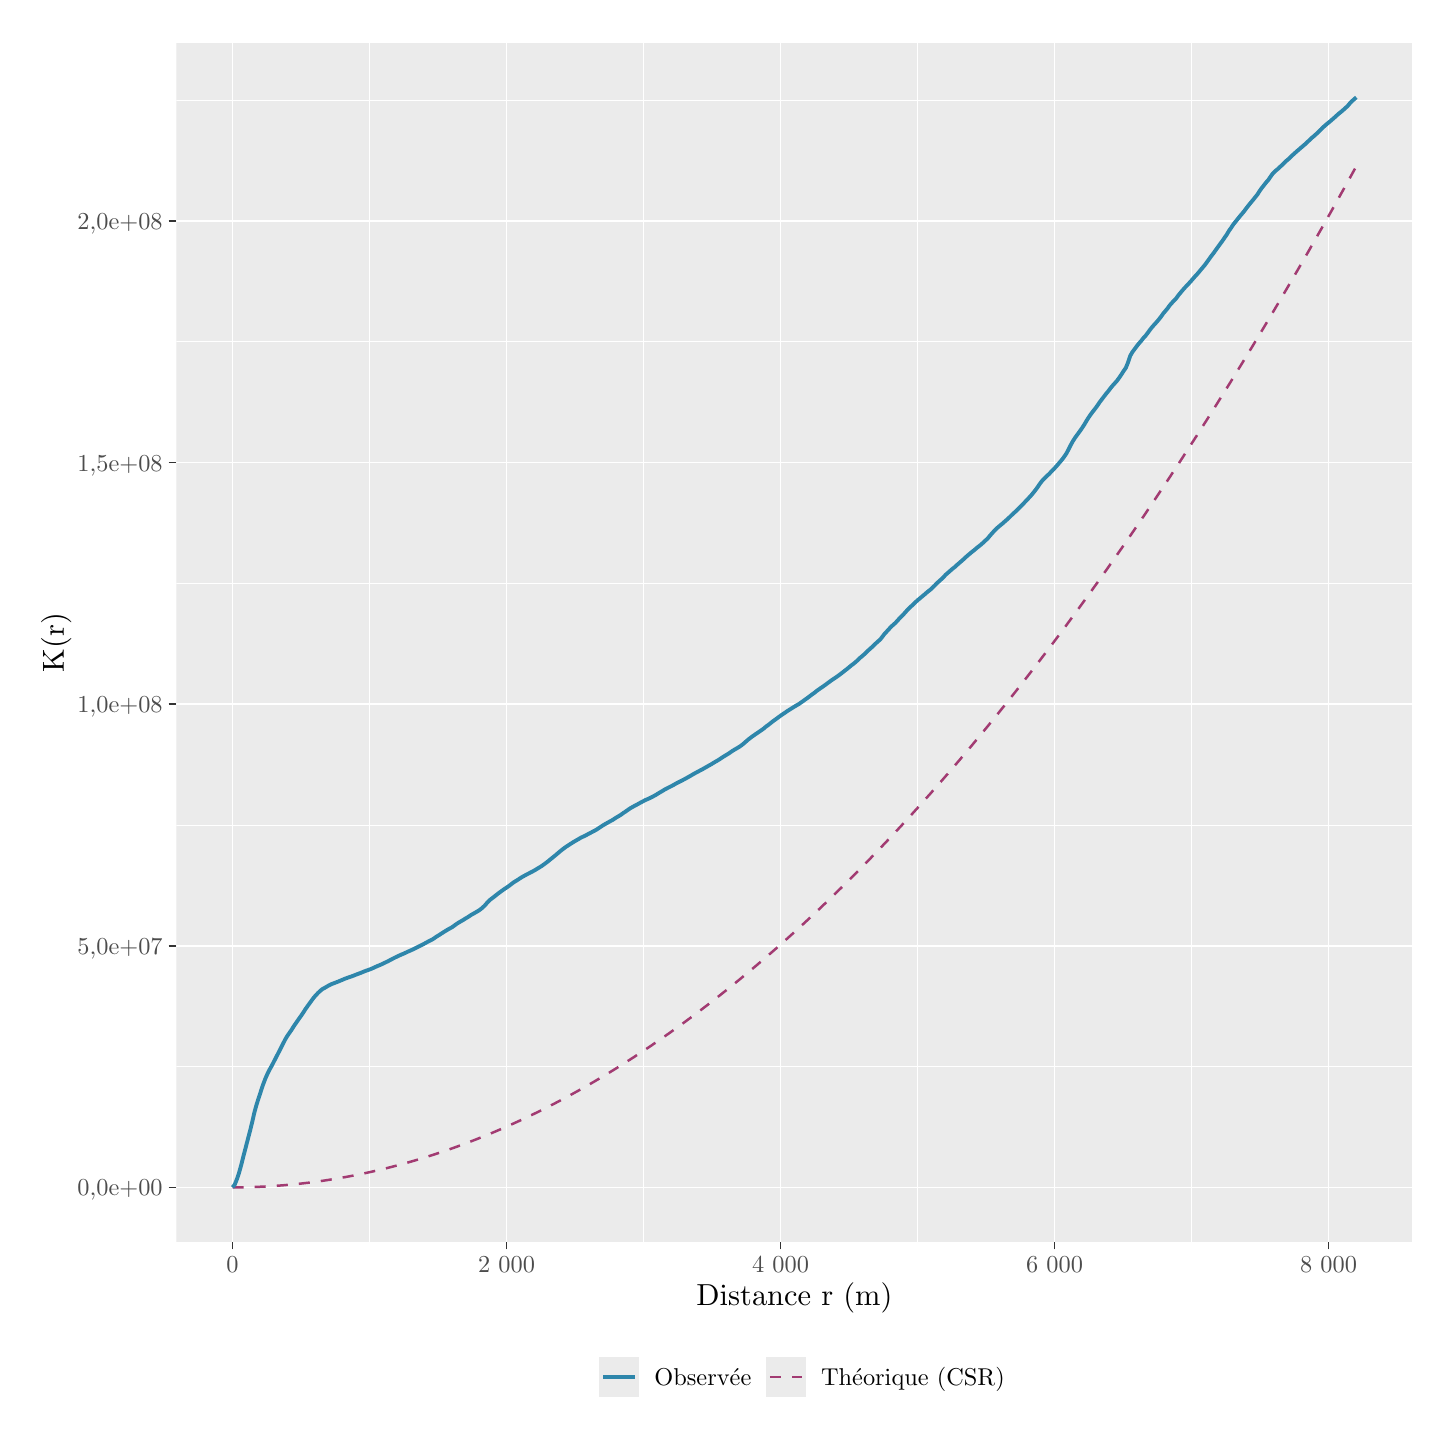
\begin{tikzpicture}[x=1pt,y=1pt]
\definecolor{fillColor}{RGB}{255,255,255}
\path[use as bounding box,fill=fillColor,fill opacity=0.00] (0,0) rectangle (505.89,505.89);
\begin{scope}
\path[clip] (  0.00,  0.00) rectangle (505.89,505.89);
\definecolor{drawColor}{RGB}{255,255,255}
\definecolor{fillColor}{RGB}{255,255,255}

\path[draw=drawColor,line width= 0.6pt,line join=round,line cap=round,fill=fillColor] (  0.00,  0.00) rectangle (505.89,505.89);
\end{scope}
\begin{scope}
\path[clip] ( 53.72, 67.14) rectangle (500.39,500.39);
\definecolor{fillColor}{gray}{0.92}

\path[fill=fillColor] ( 53.72, 67.14) rectangle (500.39,500.39);
\definecolor{drawColor}{RGB}{255,255,255}

\path[draw=drawColor,line width= 0.3pt,line join=round] ( 53.72,130.48) --
	(500.39,130.48);

\path[draw=drawColor,line width= 0.3pt,line join=round] ( 53.72,217.77) --
	(500.39,217.77);

\path[draw=drawColor,line width= 0.3pt,line join=round] ( 53.72,305.06) --
	(500.39,305.06);

\path[draw=drawColor,line width= 0.3pt,line join=round] ( 53.72,392.34) --
	(500.39,392.34);

\path[draw=drawColor,line width= 0.3pt,line join=round] ( 53.72,479.63) --
	(500.39,479.63);

\path[draw=drawColor,line width= 0.3pt,line join=round] (123.53, 67.14) --
	(123.53,500.39);

\path[draw=drawColor,line width= 0.3pt,line join=round] (222.54, 67.14) --
	(222.54,500.39);

\path[draw=drawColor,line width= 0.3pt,line join=round] (321.56, 67.14) --
	(321.56,500.39);

\path[draw=drawColor,line width= 0.3pt,line join=round] (420.58, 67.14) --
	(420.58,500.39);

\path[draw=drawColor,line width= 0.6pt,line join=round] ( 53.72, 86.84) --
	(500.39, 86.84);

\path[draw=drawColor,line width= 0.6pt,line join=round] ( 53.72,174.12) --
	(500.39,174.12);

\path[draw=drawColor,line width= 0.6pt,line join=round] ( 53.72,261.41) --
	(500.39,261.41);

\path[draw=drawColor,line width= 0.6pt,line join=round] ( 53.72,348.70) --
	(500.39,348.70);

\path[draw=drawColor,line width= 0.6pt,line join=round] ( 53.72,435.99) --
	(500.39,435.99);

\path[draw=drawColor,line width= 0.6pt,line join=round] ( 74.02, 67.14) --
	( 74.02,500.39);

\path[draw=drawColor,line width= 0.6pt,line join=round] (173.04, 67.14) --
	(173.04,500.39);

\path[draw=drawColor,line width= 0.6pt,line join=round] (272.05, 67.14) --
	(272.05,500.39);

\path[draw=drawColor,line width= 0.6pt,line join=round] (371.07, 67.14) --
	(371.07,500.39);

\path[draw=drawColor,line width= 0.6pt,line join=round] (470.09, 67.14) --
	(470.09,500.39);
\definecolor{drawColor}{RGB}{162,59,114}

\path[draw=drawColor,line width= 0.9pt,dash pattern=on 4pt off 4pt ,line join=round] ( 74.02, 86.84) --
	( 74.81, 86.84) --
	( 75.61, 86.84) --
	( 76.40, 86.85) --
	( 77.19, 86.86) --
	( 77.99, 86.87) --
	( 78.78, 86.89) --
	( 79.57, 86.91) --
	( 80.37, 86.93) --
	( 81.16, 86.95) --
	( 81.95, 86.98) --
	( 82.74, 87.01) --
	( 83.54, 87.04) --
	( 84.33, 87.07) --
	( 85.12, 87.11) --
	( 85.92, 87.15) --
	( 86.71, 87.20) --
	( 87.50, 87.24) --
	( 88.30, 87.29) --
	( 89.09, 87.34) --
	( 89.88, 87.40) --
	( 90.68, 87.46) --
	( 91.47, 87.52) --
	( 92.26, 87.58) --
	( 93.05, 87.65) --
	( 93.85, 87.72) --
	( 94.64, 87.79) --
	( 95.43, 87.86) --
	( 96.23, 87.94) --
	( 97.02, 88.02) --
	( 97.81, 88.10) --
	( 98.61, 88.19) --
	( 99.40, 88.28) --
	(100.19, 88.37) --
	(100.99, 88.46) --
	(101.78, 88.56) --
	(102.57, 88.66) --
	(103.36, 88.76) --
	(104.16, 88.87) --
	(104.95, 88.98) --
	(105.74, 89.09) --
	(106.54, 89.20) --
	(107.33, 89.32) --
	(108.12, 89.44) --
	(108.92, 89.56) --
	(109.71, 89.69) --
	(110.50, 89.81) --
	(111.30, 89.95) --
	(112.09, 90.08) --
	(112.88, 90.22) --
	(113.68, 90.36) --
	(114.47, 90.50) --
	(115.26, 90.64) --
	(116.05, 90.79) --
	(116.85, 90.94) --
	(117.64, 91.09) --
	(118.43, 91.25) --
	(119.23, 91.41) --
	(120.02, 91.57) --
	(120.81, 91.74) --
	(121.61, 91.90) --
	(122.40, 92.07) --
	(123.19, 92.25) --
	(123.99, 92.42) --
	(124.78, 92.60) --
	(125.57, 92.78) --
	(126.36, 92.97) --
	(127.16, 93.15) --
	(127.95, 93.34) --
	(128.74, 93.54) --
	(129.54, 93.73) --
	(130.33, 93.93) --
	(131.12, 94.13) --
	(131.92, 94.34) --
	(132.71, 94.54) --
	(133.50, 94.75) --
	(134.30, 94.97) --
	(135.09, 95.18) --
	(135.88, 95.40) --
	(136.67, 95.62) --
	(137.47, 95.84) --
	(138.26, 96.07) --
	(139.05, 96.30) --
	(139.85, 96.53) --
	(140.64, 96.77) --
	(141.43, 97.01) --
	(142.23, 97.25) --
	(143.02, 97.49) --
	(143.81, 97.74) --
	(144.61, 97.99) --
	(145.40, 98.24) --
	(146.19, 98.49) --
	(146.99, 98.75) --
	(147.78, 99.01) --
	(148.57, 99.27) --
	(149.36, 99.54) --
	(150.16, 99.81) --
	(150.95,100.08) --
	(151.74,100.35) --
	(152.54,100.63) --
	(153.33,100.91) --
	(154.12,101.19) --
	(154.92,101.48) --
	(155.71,101.77) --
	(156.50,102.06) --
	(157.30,102.35) --
	(158.09,102.65) --
	(158.88,102.95) --
	(159.67,103.25) --
	(160.47,103.56) --
	(161.26,103.87) --
	(162.05,104.18) --
	(162.85,104.49) --
	(163.64,104.81) --
	(164.43,105.13) --
	(165.23,105.45) --
	(166.02,105.78) --
	(166.81,106.10) --
	(167.61,106.43) --
	(168.40,106.77) --
	(169.19,107.10) --
	(169.99,107.44) --
	(170.78,107.79) --
	(171.57,108.13) --
	(172.36,108.48) --
	(173.16,108.83) --
	(173.95,109.18) --
	(174.74,109.54) --
	(175.54,109.90) --
	(176.33,110.26) --
	(177.12,110.62) --
	(177.92,110.99) --
	(178.71,111.36) --
	(179.50,111.73) --
	(180.30,112.11) --
	(181.09,112.49) --
	(181.88,112.87) --
	(182.67,113.25) --
	(183.47,113.64) --
	(184.26,114.03) --
	(185.05,114.42) --
	(185.85,114.82) --
	(186.64,115.22) --
	(187.43,115.62) --
	(188.23,116.02) --
	(189.02,116.43) --
	(189.81,116.84) --
	(190.61,117.25) --
	(191.40,117.67) --
	(192.19,118.08) --
	(192.98,118.50) --
	(193.78,118.93) --
	(194.57,119.35) --
	(195.36,119.78) --
	(196.16,120.22) --
	(196.95,120.65) --
	(197.74,121.09) --
	(198.54,121.53) --
	(199.33,121.97) --
	(200.12,122.42) --
	(200.92,122.87) --
	(201.71,123.32) --
	(202.50,123.77) --
	(203.30,124.23) --
	(204.09,124.69) --
	(204.88,125.15) --
	(205.67,125.62) --
	(206.47,126.09) --
	(207.26,126.56) --
	(208.05,127.03) --
	(208.85,127.51) --
	(209.64,127.99) --
	(210.43,128.47) --
	(211.23,128.96) --
	(212.02,129.45) --
	(212.81,129.94) --
	(213.61,130.43) --
	(214.40,130.93) --
	(215.19,131.43) --
	(215.98,131.93) --
	(216.78,132.44) --
	(217.57,132.95) --
	(218.36,133.46) --
	(219.16,133.97) --
	(219.95,134.49) --
	(220.74,135.01) --
	(221.54,135.53) --
	(222.33,136.05) --
	(223.12,136.58) --
	(223.92,137.11) --
	(224.71,137.65) --
	(225.50,138.18) --
	(226.30,138.72) --
	(227.09,139.26) --
	(227.88,139.81) --
	(228.67,140.35) --
	(229.47,140.91) --
	(230.26,141.46) --
	(231.05,142.01) --
	(231.85,142.57) --
	(232.64,143.13) --
	(233.43,143.70) --
	(234.23,144.27) --
	(235.02,144.84) --
	(235.81,145.41) --
	(236.61,145.98) --
	(237.40,146.56) --
	(238.19,147.14) --
	(238.98,147.73) --
	(239.78,148.32) --
	(240.57,148.91) --
	(241.36,149.50) --
	(242.16,150.09) --
	(242.95,150.69) --
	(243.74,151.29) --
	(244.54,151.90) --
	(245.33,152.50) --
	(246.12,153.11) --
	(246.92,153.72) --
	(247.71,154.34) --
	(248.50,154.96) --
	(249.29,155.58) --
	(250.09,156.20) --
	(250.88,156.83) --
	(251.67,157.46) --
	(252.47,158.09) --
	(253.26,158.72) --
	(254.05,159.36) --
	(254.85,160.00) --
	(255.64,160.64) --
	(256.43,161.29) --
	(257.23,161.94) --
	(258.02,162.59) --
	(258.81,163.25) --
	(259.61,163.90) --
	(260.40,164.56) --
	(261.19,165.23) --
	(261.98,165.89) --
	(262.78,166.56) --
	(263.57,167.23) --
	(264.36,167.91) --
	(265.16,168.58) --
	(265.95,169.26) --
	(266.74,169.94) --
	(267.54,170.63) --
	(268.33,171.32) --
	(269.12,172.01) --
	(269.92,172.70) --
	(270.71,173.40) --
	(271.50,174.10) --
	(272.29,174.80) --
	(273.09,175.51) --
	(273.88,176.22) --
	(274.67,176.93) --
	(275.47,177.64) --
	(276.26,178.36) --
	(277.05,179.08) --
	(277.85,179.80) --
	(278.64,180.52) --
	(279.43,181.25) --
	(280.23,181.98) --
	(281.02,182.71) --
	(281.81,183.45) --
	(282.61,184.19) --
	(283.40,184.93) --
	(284.19,185.67) --
	(284.98,186.42) --
	(285.78,187.17) --
	(286.57,187.93) --
	(287.36,188.68) --
	(288.16,189.44) --
	(288.95,190.20) --
	(289.74,190.97) --
	(290.54,191.73) --
	(291.33,192.50) --
	(292.12,193.27) --
	(292.92,194.05) --
	(293.71,194.83) --
	(294.50,195.61) --
	(295.29,196.39) --
	(296.09,197.18) --
	(296.88,197.97) --
	(297.67,198.76) --
	(298.47,199.56) --
	(299.26,200.36) --
	(300.05,201.16) --
	(300.85,201.96) --
	(301.64,202.77) --
	(302.43,203.58) --
	(303.23,204.39) --
	(304.02,205.20) --
	(304.81,206.02) --
	(305.60,206.84) --
	(306.40,207.66) --
	(307.19,208.49) --
	(307.98,209.32) --
	(308.78,210.15) --
	(309.57,210.99) --
	(310.36,211.82) --
	(311.16,212.66) --
	(311.95,213.51) --
	(312.74,214.35) --
	(313.54,215.20) --
	(314.33,216.05) --
	(315.12,216.91) --
	(315.92,217.76) --
	(316.71,218.62) --
	(317.50,219.49) --
	(318.29,220.35) --
	(319.09,221.22) --
	(319.88,222.09) --
	(320.67,222.97) --
	(321.47,223.84) --
	(322.26,224.72) --
	(323.05,225.61) --
	(323.85,226.49) --
	(324.64,227.38) --
	(325.43,228.27) --
	(326.23,229.16) --
	(327.02,230.06) --
	(327.81,230.96) --
	(328.60,231.86) --
	(329.40,232.77) --
	(330.19,233.67) --
	(330.98,234.58) --
	(331.78,235.50) --
	(332.57,236.41) --
	(333.36,237.33) --
	(334.16,238.26) --
	(334.95,239.18) --
	(335.74,240.11) --
	(336.54,241.04) --
	(337.33,241.97) --
	(338.12,242.91) --
	(338.92,243.85) --
	(339.71,244.79) --
	(340.50,245.73) --
	(341.29,246.68) --
	(342.09,247.63) --
	(342.88,248.58) --
	(343.67,249.54) --
	(344.47,250.50) --
	(345.26,251.46) --
	(346.05,252.42) --
	(346.85,253.39) --
	(347.64,254.36) --
	(348.43,255.33) --
	(349.23,256.31) --
	(350.02,257.28) --
	(350.81,258.26) --
	(351.60,259.25) --
	(352.40,260.24) --
	(353.19,261.22) --
	(353.98,262.22) --
	(354.78,263.21) --
	(355.57,264.21) --
	(356.36,265.21) --
	(357.16,266.21) --
	(357.95,267.22) --
	(358.74,268.23) --
	(359.54,269.24) --
	(360.33,270.26) --
	(361.12,271.27) --
	(361.91,272.29) --
	(362.71,273.32) --
	(363.50,274.34) --
	(364.29,275.37) --
	(365.09,276.40) --
	(365.88,277.44) --
	(366.67,278.48) --
	(367.47,279.52) --
	(368.26,280.56) --
	(369.05,281.60) --
	(369.85,282.65) --
	(370.64,283.70) --
	(371.43,284.76) --
	(372.23,285.82) --
	(373.02,286.88) --
	(373.81,287.94) --
	(374.60,289.00) --
	(375.40,290.07) --
	(376.19,291.14) --
	(376.98,292.22) --
	(377.78,293.29) --
	(378.57,294.37) --
	(379.36,295.46) --
	(380.16,296.54) --
	(380.95,297.63) --
	(381.74,298.72) --
	(382.54,299.81) --
	(383.33,300.91) --
	(384.12,302.01) --
	(384.91,303.11) --
	(385.71,304.22) --
	(386.50,305.32) --
	(387.29,306.43) --
	(388.09,307.55) --
	(388.88,308.66) --
	(389.67,309.78) --
	(390.47,310.90) --
	(391.26,312.03) --
	(392.05,313.16) --
	(392.85,314.29) --
	(393.64,315.42) --
	(394.43,316.55) --
	(395.23,317.69) --
	(396.02,318.83) --
	(396.81,319.98) --
	(397.60,321.13) --
	(398.40,322.28) --
	(399.19,323.43) --
	(399.98,324.58) --
	(400.78,325.74) --
	(401.57,326.90) --
	(402.36,328.07) --
	(403.16,329.23) --
	(403.95,330.40) --
	(404.74,331.58) --
	(405.54,332.75) --
	(406.33,333.93) --
	(407.12,335.11) --
	(407.91,336.29) --
	(408.71,337.48) --
	(409.50,338.67) --
	(410.29,339.86) --
	(411.09,341.06) --
	(411.88,342.25) --
	(412.67,343.45) --
	(413.47,344.66) --
	(414.26,345.86) --
	(415.05,347.07) --
	(415.85,348.29) --
	(416.64,349.50) --
	(417.43,350.72) --
	(418.22,351.94) --
	(419.02,353.16) --
	(419.81,354.39) --
	(420.60,355.62) --
	(421.40,356.85) --
	(422.19,358.08) --
	(422.98,359.32) --
	(423.78,360.56) --
	(424.57,361.80) --
	(425.36,363.05) --
	(426.16,364.29) --
	(426.95,365.55) --
	(427.74,366.80) --
	(428.54,368.06) --
	(429.33,369.32) --
	(430.12,370.58) --
	(430.91,371.84) --
	(431.71,373.11) --
	(432.50,374.38) --
	(433.29,375.66) --
	(434.09,376.93) --
	(434.88,378.21) --
	(435.67,379.50) --
	(436.47,380.78) --
	(437.26,382.07) --
	(438.05,383.36) --
	(438.85,384.65) --
	(439.64,385.95) --
	(440.43,387.25) --
	(441.22,388.55) --
	(442.02,389.85) --
	(442.81,391.16) --
	(443.60,392.47) --
	(444.40,393.78) --
	(445.19,395.10) --
	(445.98,396.42) --
	(446.78,397.74) --
	(447.57,399.07) --
	(448.36,400.39) --
	(449.16,401.72) --
	(449.95,403.06) --
	(450.74,404.39) --
	(451.54,405.73) --
	(452.33,407.07) --
	(453.12,408.42) --
	(453.91,409.76) --
	(454.71,411.11) --
	(455.50,412.46) --
	(456.29,413.82) --
	(457.09,415.18) --
	(457.88,416.54) --
	(458.67,417.90) --
	(459.47,419.27) --
	(460.26,420.64) --
	(461.05,422.01) --
	(461.85,423.39) --
	(462.64,424.76) --
	(463.43,426.14) --
	(464.22,427.53) --
	(465.02,428.91) --
	(465.81,430.30) --
	(466.60,431.70) --
	(467.40,433.09) --
	(468.19,434.49) --
	(468.98,435.89) --
	(469.78,437.29) --
	(470.57,438.70) --
	(471.36,440.11) --
	(472.16,441.52) --
	(472.95,442.93) --
	(473.74,444.35) --
	(474.53,445.77) --
	(475.33,447.19) --
	(476.12,448.62) --
	(476.91,450.05) --
	(477.71,451.48) --
	(478.50,452.91) --
	(479.29,454.35) --
	(480.09,455.79);
\definecolor{drawColor}{RGB}{46,134,171}

\path[draw=drawColor,line width= 1.4pt,line join=round] ( 74.02, 86.84) --
	( 74.81, 87.81) --
	( 75.61, 89.81) --
	( 76.40, 92.18) --
	( 77.19, 95.01) --
	( 77.99, 98.22) --
	( 78.78,101.23) --
	( 79.57,104.28) --
	( 80.37,107.32) --
	( 81.16,110.54) --
	( 81.95,114.02) --
	( 82.74,116.85) --
	( 83.54,119.36) --
	( 84.33,121.76) --
	( 85.12,124.13) --
	( 85.92,126.22) --
	( 86.71,128.00) --
	( 87.50,129.54) --
	( 88.30,130.97) --
	( 89.09,132.51) --
	( 89.88,134.05) --
	( 90.68,135.60) --
	( 91.47,137.12) --
	( 92.26,138.72) --
	( 93.05,140.25) --
	( 93.85,141.61) --
	( 94.64,142.73) --
	( 95.43,143.87) --
	( 96.23,145.18) --
	( 97.02,146.30) --
	( 97.81,147.45) --
	( 98.61,148.57) --
	( 99.40,149.72) --
	(100.19,150.95) --
	(100.99,152.13) --
	(101.78,153.21) --
	(102.57,154.30) --
	(103.36,155.38) --
	(104.16,156.29) --
	(104.95,157.12) --
	(105.74,157.87) --
	(106.54,158.51) --
	(107.33,158.92) --
	(108.12,159.39) --
	(108.92,159.85) --
	(109.71,160.25) --
	(110.50,160.54) --
	(111.30,160.85) --
	(112.09,161.15) --
	(112.88,161.49) --
	(113.68,161.81) --
	(114.47,162.16) --
	(115.26,162.45) --
	(116.05,162.75) --
	(116.85,163.01) --
	(117.64,163.29) --
	(118.43,163.61) --
	(119.23,163.92) --
	(120.02,164.21) --
	(120.81,164.52) --
	(121.61,164.86) --
	(122.40,165.16) --
	(123.19,165.43) --
	(123.99,165.73) --
	(124.78,166.07) --
	(125.57,166.44) --
	(126.36,166.79) --
	(127.16,167.13) --
	(127.95,167.47) --
	(128.74,167.86) --
	(129.54,168.23) --
	(130.33,168.61) --
	(131.12,169.05) --
	(131.92,169.46) --
	(132.71,169.86) --
	(133.50,170.24) --
	(134.30,170.62) --
	(135.09,170.97) --
	(135.88,171.30) --
	(136.67,171.67) --
	(137.47,172.05) --
	(138.26,172.39) --
	(139.05,172.74) --
	(139.85,173.13) --
	(140.64,173.52) --
	(141.43,173.93) --
	(142.23,174.34) --
	(143.02,174.73) --
	(143.81,175.16) --
	(144.61,175.60) --
	(145.40,176.00) --
	(146.19,176.40) --
	(146.99,176.92) --
	(147.78,177.47) --
	(148.57,177.94) --
	(149.36,178.46) --
	(150.16,178.97) --
	(150.95,179.47) --
	(151.74,179.95) --
	(152.54,180.40) --
	(153.33,180.82) --
	(154.12,181.38) --
	(154.92,181.98) --
	(155.71,182.50) --
	(156.50,182.95) --
	(157.30,183.41) --
	(158.09,183.92) --
	(158.88,184.38) --
	(159.67,184.88) --
	(160.47,185.41) --
	(161.26,185.84) --
	(162.05,186.30) --
	(162.85,186.77) --
	(163.64,187.31) --
	(164.43,187.97) --
	(165.23,188.74) --
	(166.02,189.68) --
	(166.81,190.50) --
	(167.61,191.15) --
	(168.40,191.73) --
	(169.19,192.37) --
	(169.99,192.99) --
	(170.78,193.59) --
	(171.57,194.15) --
	(172.36,194.72) --
	(173.16,195.24) --
	(173.95,195.78) --
	(174.74,196.40) --
	(175.54,197.00) --
	(176.33,197.50) --
	(177.12,197.98) --
	(177.92,198.52) --
	(178.71,199.01) --
	(179.50,199.44) --
	(180.30,199.89) --
	(181.09,200.28) --
	(181.88,200.71) --
	(182.67,201.11) --
	(183.47,201.56) --
	(184.26,202.06) --
	(185.05,202.52) --
	(185.85,203.04) --
	(186.64,203.60) --
	(187.43,204.19) --
	(188.23,204.81) --
	(189.02,205.46) --
	(189.81,206.11) --
	(190.61,206.75) --
	(191.40,207.42) --
	(192.19,208.10) --
	(192.98,208.74) --
	(193.78,209.35) --
	(194.57,209.93) --
	(195.36,210.42) --
	(196.16,210.95) --
	(196.95,211.46) --
	(197.74,211.93) --
	(198.54,212.39) --
	(199.33,212.85) --
	(200.12,213.30) --
	(200.92,213.66) --
	(201.71,214.04) --
	(202.50,214.49) --
	(203.30,214.90) --
	(204.09,215.32) --
	(204.88,215.73) --
	(205.67,216.18) --
	(206.47,216.71) --
	(207.26,217.23) --
	(208.05,217.76) --
	(208.85,218.20) --
	(209.64,218.65) --
	(210.43,219.10) --
	(211.23,219.52) --
	(212.02,220.02) --
	(212.81,220.54) --
	(213.61,221.00) --
	(214.40,221.50) --
	(215.19,222.07) --
	(215.98,222.59) --
	(216.78,223.15) --
	(217.57,223.71) --
	(218.36,224.17) --
	(219.16,224.61) --
	(219.95,225.03) --
	(220.74,225.46) --
	(221.54,225.91) --
	(222.33,226.32) --
	(223.12,226.74) --
	(223.92,227.09) --
	(224.71,227.45) --
	(225.50,227.83) --
	(226.30,228.26) --
	(227.09,228.70) --
	(227.88,229.20) --
	(228.67,229.67) --
	(229.47,230.13) --
	(230.26,230.63) --
	(231.05,231.04) --
	(231.85,231.44) --
	(232.64,231.84) --
	(233.43,232.26) --
	(234.23,232.73) --
	(235.02,233.14) --
	(235.81,233.55) --
	(236.61,233.95) --
	(237.40,234.36) --
	(238.19,234.80) --
	(238.98,235.24) --
	(239.78,235.70) --
	(240.57,236.18) --
	(241.36,236.61) --
	(242.16,237.02) --
	(242.95,237.46) --
	(243.74,237.86) --
	(244.54,238.33) --
	(245.33,238.77) --
	(246.12,239.23) --
	(246.92,239.66) --
	(247.71,240.16) --
	(248.50,240.63) --
	(249.29,241.08) --
	(250.09,241.58) --
	(250.88,242.12) --
	(251.67,242.61) --
	(252.47,243.10) --
	(253.26,243.57) --
	(254.05,244.12) --
	(254.85,244.66) --
	(255.64,245.14) --
	(256.43,245.58) --
	(257.23,246.08) --
	(258.02,246.62) --
	(258.81,247.29) --
	(259.61,247.99) --
	(260.40,248.67) --
	(261.19,249.28) --
	(261.98,249.87) --
	(262.78,250.42) --
	(263.57,250.97) --
	(264.36,251.50) --
	(265.16,252.05) --
	(265.95,252.61) --
	(266.74,253.30) --
	(267.54,253.87) --
	(268.33,254.48) --
	(269.12,255.13) --
	(269.92,255.70) --
	(270.71,256.28) --
	(271.50,256.86) --
	(272.29,257.44) --
	(273.09,257.98) --
	(273.88,258.51) --
	(274.67,259.05) --
	(275.47,259.55) --
	(276.26,260.05) --
	(277.05,260.54) --
	(277.85,261.01) --
	(278.64,261.47) --
	(279.43,262.01) --
	(280.23,262.58) --
	(281.02,263.16) --
	(281.81,263.71) --
	(282.61,264.32) --
	(283.40,264.93) --
	(284.19,265.47) --
	(284.98,266.13) --
	(285.78,266.71) --
	(286.57,267.25) --
	(287.36,267.79) --
	(288.16,268.35) --
	(288.95,268.95) --
	(289.74,269.53) --
	(290.54,270.11) --
	(291.33,270.64) --
	(292.12,271.16) --
	(292.92,271.73) --
	(293.71,272.32) --
	(294.50,272.93) --
	(295.29,273.57) --
	(296.09,274.17) --
	(296.88,274.82) --
	(297.67,275.49) --
	(298.47,276.07) --
	(299.26,276.74) --
	(300.05,277.45) --
	(300.85,278.22) --
	(301.64,278.88) --
	(302.43,279.58) --
	(303.23,280.35) --
	(304.02,281.11) --
	(304.81,281.81) --
	(305.60,282.54) --
	(306.40,283.32) --
	(307.19,284.07) --
	(307.98,284.71) --
	(308.78,285.72) --
	(309.57,286.76) --
	(310.36,287.62) --
	(311.16,288.49) --
	(311.95,289.38) --
	(312.74,290.08) --
	(313.54,290.79) --
	(314.33,291.64) --
	(315.12,292.55) --
	(315.92,293.33) --
	(316.71,294.15) --
	(317.50,295.04) --
	(318.29,295.91) --
	(319.09,296.66) --
	(319.88,297.36) --
	(320.67,298.15) --
	(321.47,298.90) --
	(322.26,299.56) --
	(323.05,300.22) --
	(323.85,300.88) --
	(324.64,301.57) --
	(325.43,302.23) --
	(326.23,302.85) --
	(327.02,303.58) --
	(327.81,304.36) --
	(328.60,305.20) --
	(329.40,305.90) --
	(330.19,306.63) --
	(330.98,307.41) --
	(331.78,308.26) --
	(332.57,308.94) --
	(333.36,309.64) --
	(334.16,310.34) --
	(334.95,310.95) --
	(335.74,311.68) --
	(336.54,312.37) --
	(337.33,313.05) --
	(338.12,313.75) --
	(338.92,314.50) --
	(339.71,315.20) --
	(340.50,315.85) --
	(341.29,316.52) --
	(342.09,317.14) --
	(342.88,317.84) --
	(343.67,318.45) --
	(344.47,319.08) --
	(345.26,319.80) --
	(346.05,320.54) --
	(346.85,321.27) --
	(347.64,322.22) --
	(348.43,323.14) --
	(349.23,324.00) --
	(350.02,324.81) --
	(350.81,325.53) --
	(351.60,326.18) --
	(352.40,326.83) --
	(353.19,327.55) --
	(353.98,328.22) --
	(354.78,328.98) --
	(355.57,329.77) --
	(356.36,330.50) --
	(357.16,331.23) --
	(357.95,331.99) --
	(358.74,332.81) --
	(359.54,333.63) --
	(360.33,334.44) --
	(361.12,335.28) --
	(361.91,336.12) --
	(362.71,337.00) --
	(363.50,337.96) --
	(364.29,338.98) --
	(365.09,340.07) --
	(365.88,341.25) --
	(366.67,342.27) --
	(367.47,343.05) --
	(368.26,343.87) --
	(369.05,344.57) --
	(369.85,345.44) --
	(370.64,346.23) --
	(371.43,347.09) --
	(372.23,347.99) --
	(373.02,348.94) --
	(373.81,349.85) --
	(374.60,350.94) --
	(375.40,352.13) --
	(376.19,353.63) --
	(376.98,355.21) --
	(377.78,356.65) --
	(378.57,357.85) --
	(379.36,358.92) --
	(380.16,360.02) --
	(380.95,361.14) --
	(381.74,362.35) --
	(382.54,363.71) --
	(383.33,364.99) --
	(384.12,366.13) --
	(384.91,367.19) --
	(385.71,368.20) --
	(386.50,369.27) --
	(387.29,370.46) --
	(388.09,371.51) --
	(388.88,372.55) --
	(389.67,373.58) --
	(390.47,374.53) --
	(391.26,375.58) --
	(392.05,376.55) --
	(392.85,377.43) --
	(393.64,378.32) --
	(394.43,379.41) --
	(395.23,380.57) --
	(396.02,381.83) --
	(396.81,382.95) --
	(397.60,384.90) --
	(398.40,387.30) --
	(399.19,388.68) --
	(399.98,389.72) --
	(400.78,390.82) --
	(401.57,391.80) --
	(402.36,392.70) --
	(403.16,393.72) --
	(403.95,394.58) --
	(404.74,395.60) --
	(405.54,396.71) --
	(406.33,397.71) --
	(407.12,398.61) --
	(407.91,399.47) --
	(408.71,400.42) --
	(409.50,401.41) --
	(410.29,402.54) --
	(411.09,403.48) --
	(411.88,404.43) --
	(412.67,405.55) --
	(413.47,406.45) --
	(414.26,407.28) --
	(415.05,408.13) --
	(415.85,409.24) --
	(416.64,410.18) --
	(417.43,411.13) --
	(418.22,412.02) --
	(419.02,412.84) --
	(419.81,413.71) --
	(420.60,414.59) --
	(421.40,415.54) --
	(422.19,416.40) --
	(422.98,417.26) --
	(423.78,418.25) --
	(424.57,419.17) --
	(425.36,420.12) --
	(426.16,421.22) --
	(426.95,422.32) --
	(427.74,423.42) --
	(428.54,424.45) --
	(429.33,425.56) --
	(430.12,426.67) --
	(430.91,427.75) --
	(431.71,428.84) --
	(432.50,430.00) --
	(433.29,431.13) --
	(434.09,432.50) --
	(434.88,433.59) --
	(435.67,434.79) --
	(436.47,435.80) --
	(437.26,436.78) --
	(438.05,437.77) --
	(438.85,438.70) --
	(439.64,439.66) --
	(440.43,440.74) --
	(441.22,441.74) --
	(442.02,442.73) --
	(442.81,443.67) --
	(443.60,444.67) --
	(444.40,445.65) --
	(445.19,446.93) --
	(445.98,448.02) --
	(446.78,449.03) --
	(447.57,450.03) --
	(448.36,450.94) --
	(449.16,452.12) --
	(449.95,453.23) --
	(450.74,454.01) --
	(451.54,454.66) --
	(452.33,455.38) --
	(453.12,456.12) --
	(453.91,456.92) --
	(454.71,457.67) --
	(455.50,458.33) --
	(456.29,459.05) --
	(457.09,459.85) --
	(457.88,460.56) --
	(458.67,461.28) --
	(459.47,461.95) --
	(460.26,462.64) --
	(461.05,463.31) --
	(461.85,464.00) --
	(462.64,464.76) --
	(463.43,465.52) --
	(464.22,466.24) --
	(465.02,466.89) --
	(465.81,467.64) --
	(466.60,468.39) --
	(467.40,469.15) --
	(468.19,469.97) --
	(468.98,470.66) --
	(469.78,471.35) --
	(470.57,471.98) --
	(471.36,472.67) --
	(472.16,473.37) --
	(472.95,474.09) --
	(473.74,474.80) --
	(474.53,475.42) --
	(475.33,476.10) --
	(476.12,476.82) --
	(476.91,477.53) --
	(477.71,478.49) --
	(478.50,479.29) --
	(479.29,480.02) --
	(480.09,480.70);
\end{scope}
\begin{scope}
\path[clip] (  0.00,  0.00) rectangle (505.89,505.89);
\definecolor{drawColor}{gray}{0.30}

\node[text=drawColor,anchor=base east,inner sep=0pt, outer sep=0pt, scale=  0.88] at ( 48.77, 83.81) {0,0e+00};

\node[text=drawColor,anchor=base east,inner sep=0pt, outer sep=0pt, scale=  0.88] at ( 48.77,171.09) {5,0e+07};

\node[text=drawColor,anchor=base east,inner sep=0pt, outer sep=0pt, scale=  0.88] at ( 48.77,258.38) {1,0e+08};

\node[text=drawColor,anchor=base east,inner sep=0pt, outer sep=0pt, scale=  0.88] at ( 48.77,345.67) {1,5e+08};

\node[text=drawColor,anchor=base east,inner sep=0pt, outer sep=0pt, scale=  0.88] at ( 48.77,432.96) {2,0e+08};
\end{scope}
\begin{scope}
\path[clip] (  0.00,  0.00) rectangle (505.89,505.89);
\definecolor{drawColor}{gray}{0.20}

\path[draw=drawColor,line width= 0.6pt,line join=round] ( 50.97, 86.84) --
	( 53.72, 86.84);

\path[draw=drawColor,line width= 0.6pt,line join=round] ( 50.97,174.12) --
	( 53.72,174.12);

\path[draw=drawColor,line width= 0.6pt,line join=round] ( 50.97,261.41) --
	( 53.72,261.41);

\path[draw=drawColor,line width= 0.6pt,line join=round] ( 50.97,348.70) --
	( 53.72,348.70);

\path[draw=drawColor,line width= 0.6pt,line join=round] ( 50.97,435.99) --
	( 53.72,435.99);
\end{scope}
\begin{scope}
\path[clip] (  0.00,  0.00) rectangle (505.89,505.89);
\definecolor{drawColor}{gray}{0.20}

\path[draw=drawColor,line width= 0.6pt,line join=round] ( 74.02, 64.39) --
	( 74.02, 67.14);

\path[draw=drawColor,line width= 0.6pt,line join=round] (173.04, 64.39) --
	(173.04, 67.14);

\path[draw=drawColor,line width= 0.6pt,line join=round] (272.05, 64.39) --
	(272.05, 67.14);

\path[draw=drawColor,line width= 0.6pt,line join=round] (371.07, 64.39) --
	(371.07, 67.14);

\path[draw=drawColor,line width= 0.6pt,line join=round] (470.09, 64.39) --
	(470.09, 67.14);
\end{scope}
\begin{scope}
\path[clip] (  0.00,  0.00) rectangle (505.89,505.89);
\definecolor{drawColor}{gray}{0.30}

\node[text=drawColor,anchor=base,inner sep=0pt, outer sep=0pt, scale=  0.88] at ( 74.02, 56.13) {0};

\node[text=drawColor,anchor=base,inner sep=0pt, outer sep=0pt, scale=  0.88] at (173.04, 56.13) {2 000};

\node[text=drawColor,anchor=base,inner sep=0pt, outer sep=0pt, scale=  0.88] at (272.05, 56.13) {4 000};

\node[text=drawColor,anchor=base,inner sep=0pt, outer sep=0pt, scale=  0.88] at (371.07, 56.13) {6 000};

\node[text=drawColor,anchor=base,inner sep=0pt, outer sep=0pt, scale=  0.88] at (470.09, 56.13) {8 000};
\end{scope}
\begin{scope}
\path[clip] (  0.00,  0.00) rectangle (505.89,505.89);
\definecolor{drawColor}{RGB}{0,0,0}

\node[text=drawColor,anchor=base,inner sep=0pt, outer sep=0pt, scale=  1.10] at (277.05, 44.09) {Distance r (m)};
\end{scope}
\begin{scope}
\path[clip] (  0.00,  0.00) rectangle (505.89,505.89);
\definecolor{drawColor}{RGB}{0,0,0}

\node[text=drawColor,rotate= 90.00,anchor=base,inner sep=0pt, outer sep=0pt, scale=  1.10] at ( 13.08,283.77) {K(r)};
\end{scope}
\begin{scope}
\path[clip] (  0.00,  0.00) rectangle (505.89,505.89);
\definecolor{fillColor}{RGB}{255,255,255}

\path[fill=fillColor] (195.51,  5.50) rectangle (358.60, 30.95);
\end{scope}
\begin{scope}
\path[clip] (  0.00,  0.00) rectangle (505.89,505.89);
\definecolor{fillColor}{gray}{0.92}

\path[fill=fillColor] (206.51, 11.00) rectangle (220.97, 25.45);
\definecolor{drawColor}{RGB}{46,134,171}

\path[draw=drawColor,line width= 1.4pt,line join=round] (207.96, 18.23) -- (219.52, 18.23);
\end{scope}
\begin{scope}
\path[clip] (  0.00,  0.00) rectangle (505.89,505.89);
\definecolor{fillColor}{gray}{0.92}

\path[fill=fillColor] (266.75, 11.00) rectangle (281.20, 25.45);
\definecolor{drawColor}{RGB}{162,59,114}

\path[draw=drawColor,line width= 0.9pt,dash pattern=on 4pt off 4pt ,line join=round] (268.20, 18.23) -- (279.76, 18.23);
\end{scope}
\begin{scope}
\path[clip] (  0.00,  0.00) rectangle (505.89,505.89);
\definecolor{drawColor}{RGB}{0,0,0}

\node[text=drawColor,anchor=base west,inner sep=0pt, outer sep=0pt, scale=  0.88] at (226.47, 15.20) {Observée};
\end{scope}
\begin{scope}
\path[clip] (  0.00,  0.00) rectangle (505.89,505.89);
\definecolor{drawColor}{RGB}{0,0,0}

\node[text=drawColor,anchor=base west,inner sep=0pt, outer sep=0pt, scale=  0.88] at (286.70, 15.20) {Théorique (CSR)};
\end{scope}
\end{tikzpicture}
%
        }
    \end{figure}
    \begin{figure}[H]
        \centering
        \caption{Corrélation proche}
        \resize{%
            % Created by tikzDevice version 0.12.6 on 2025-10-11 22:33:34
% !TEX encoding = UTF-8 Unicode
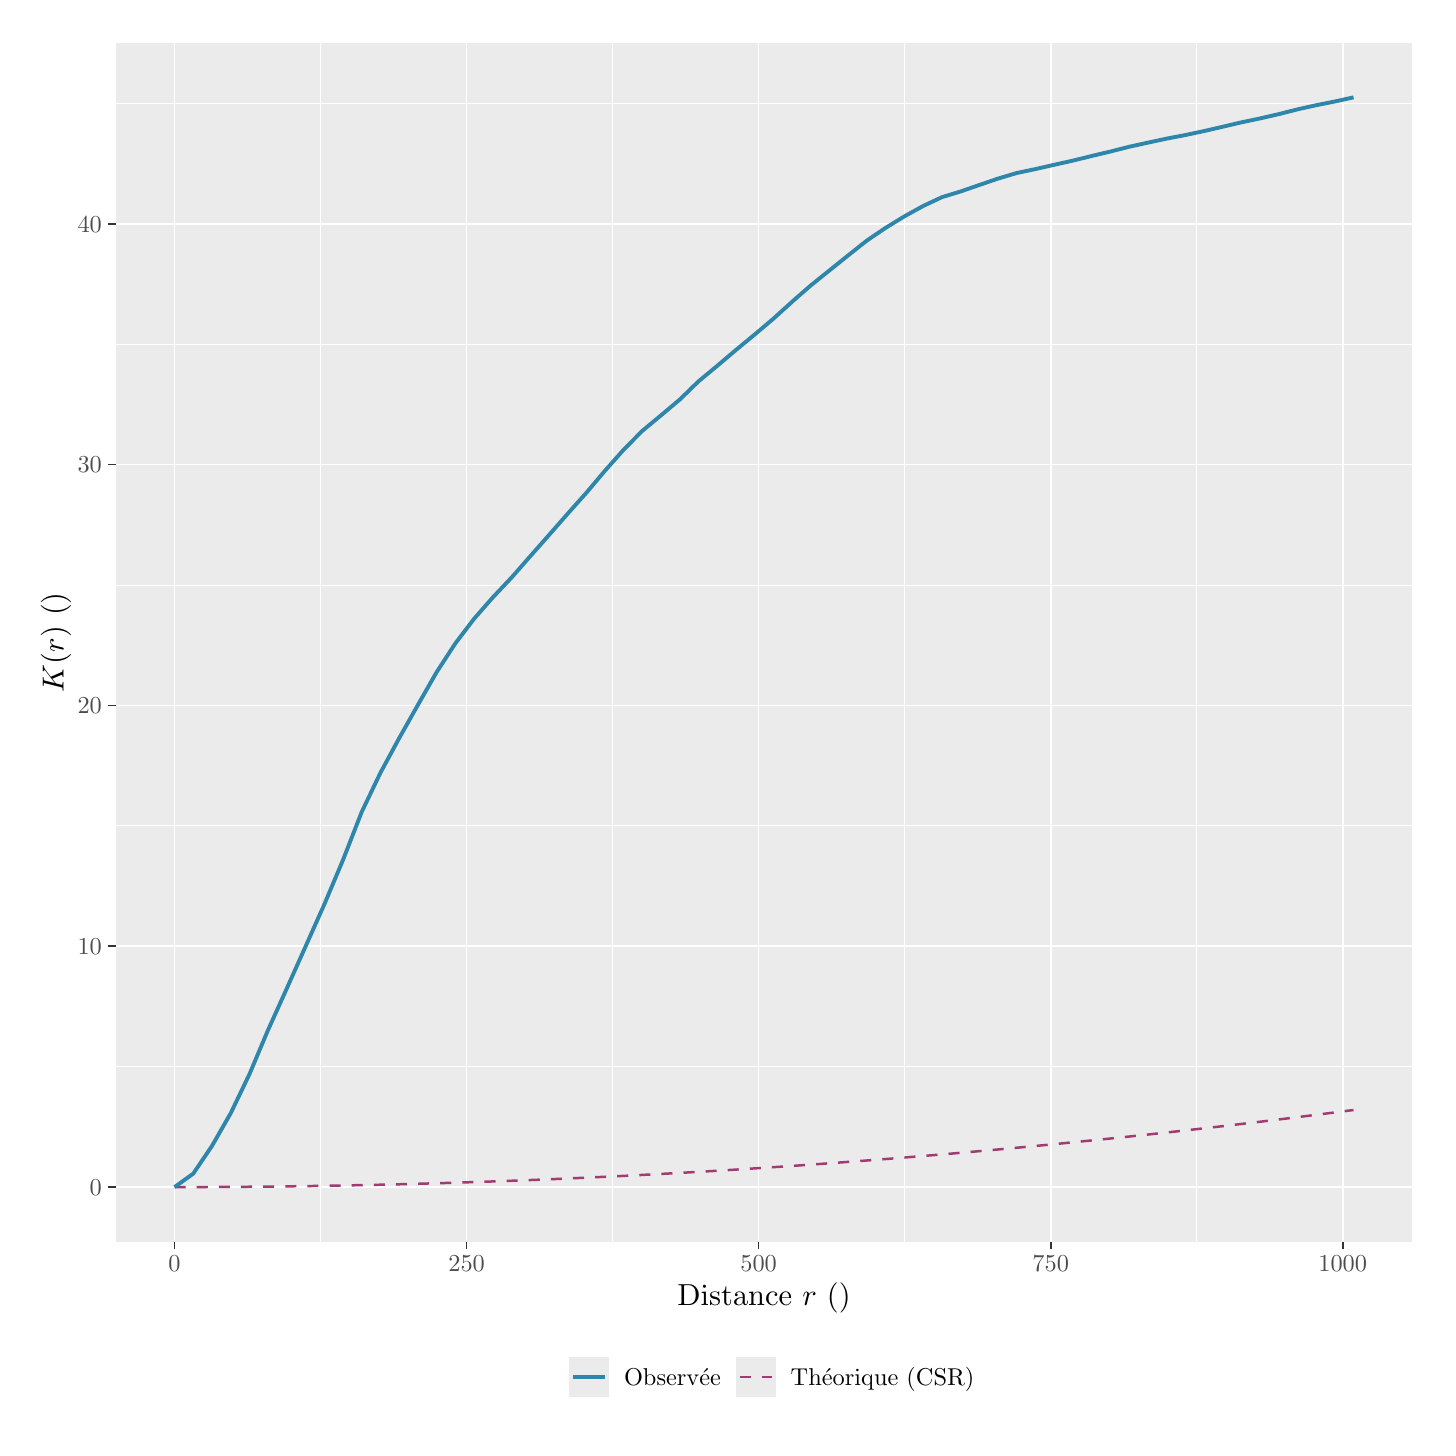
\begin{tikzpicture}[x=1pt,y=1pt]
\definecolor{fillColor}{RGB}{255,255,255}
\path[use as bounding box,fill=fillColor,fill opacity=0.00] (0,0) rectangle (505.89,505.89);
\begin{scope}
\path[clip] (  0.00,  0.00) rectangle (505.89,505.89);
\definecolor{drawColor}{RGB}{255,255,255}
\definecolor{fillColor}{RGB}{255,255,255}

\path[draw=drawColor,line width= 0.6pt,line join=round,line cap=round,fill=fillColor] (  0.00,  0.00) rectangle (505.89,505.89);
\end{scope}
\begin{scope}
\path[clip] ( 31.78, 67.26) rectangle (500.39,500.39);
\definecolor{fillColor}{gray}{0.92}

\path[fill=fillColor] ( 31.78, 67.26) rectangle (500.39,500.39);
\definecolor{drawColor}{RGB}{255,255,255}

\path[draw=drawColor,line width= 0.3pt,line join=round] ( 31.78,130.45) --
	(500.39,130.45);

\path[draw=drawColor,line width= 0.3pt,line join=round] ( 31.78,217.47) --
	(500.39,217.47);

\path[draw=drawColor,line width= 0.3pt,line join=round] ( 31.78,304.48) --
	(500.39,304.48);

\path[draw=drawColor,line width= 0.3pt,line join=round] ( 31.78,391.50) --
	(500.39,391.50);

\path[draw=drawColor,line width= 0.3pt,line join=round] ( 31.78,478.52) --
	(500.39,478.52);

\path[draw=drawColor,line width= 0.3pt,line join=round] (105.84, 67.26) --
	(105.84,500.39);

\path[draw=drawColor,line width= 0.3pt,line join=round] (211.37, 67.26) --
	(211.37,500.39);

\path[draw=drawColor,line width= 0.3pt,line join=round] (316.90, 67.26) --
	(316.90,500.39);

\path[draw=drawColor,line width= 0.3pt,line join=round] (422.43, 67.26) --
	(422.43,500.39);

\path[draw=drawColor,line width= 0.6pt,line join=round] ( 31.78, 86.94) --
	(500.39, 86.94);

\path[draw=drawColor,line width= 0.6pt,line join=round] ( 31.78,173.96) --
	(500.39,173.96);

\path[draw=drawColor,line width= 0.6pt,line join=round] ( 31.78,260.98) --
	(500.39,260.98);

\path[draw=drawColor,line width= 0.6pt,line join=round] ( 31.78,347.99) --
	(500.39,347.99);

\path[draw=drawColor,line width= 0.6pt,line join=round] ( 31.78,435.01) --
	(500.39,435.01);

\path[draw=drawColor,line width= 0.6pt,line join=round] ( 53.08, 67.26) --
	( 53.08,500.39);

\path[draw=drawColor,line width= 0.6pt,line join=round] (158.61, 67.26) --
	(158.61,500.39);

\path[draw=drawColor,line width= 0.6pt,line join=round] (264.14, 67.26) --
	(264.14,500.39);

\path[draw=drawColor,line width= 0.6pt,line join=round] (369.66, 67.26) --
	(369.66,500.39);

\path[draw=drawColor,line width= 0.6pt,line join=round] (475.19, 67.26) --
	(475.19,500.39);
\definecolor{drawColor}{RGB}{162,59,114}

\path[draw=drawColor,line width= 0.9pt,dash pattern=on 4pt off 4pt ,line join=round] ( 53.08, 86.94) --
	( 59.84, 86.95) --
	( 66.60, 86.97) --
	( 73.37, 87.01) --
	( 80.13, 87.06) --
	( 86.89, 87.12) --
	( 93.65, 87.20) --
	(100.41, 87.29) --
	(107.18, 87.39) --
	(113.94, 87.51) --
	(120.70, 87.65) --
	(127.46, 87.79) --
	(134.22, 87.95) --
	(140.99, 88.13) --
	(147.75, 88.32) --
	(154.51, 88.52) --
	(161.27, 88.74) --
	(168.03, 88.97) --
	(174.80, 89.22) --
	(181.56, 89.48) --
	(188.32, 89.75) --
	(195.08, 90.04) --
	(201.84, 90.34) --
	(208.61, 90.66) --
	(215.37, 90.98) --
	(222.13, 91.33) --
	(228.89, 91.69) --
	(235.66, 92.06) --
	(242.42, 92.44) --
	(249.18, 92.84) --
	(255.94, 93.26) --
	(262.70, 93.69) --
	(269.47, 94.13) --
	(276.23, 94.58) --
	(282.99, 95.05) --
	(289.75, 95.54) --
	(296.51, 96.04) --
	(303.28, 96.55) --
	(310.04, 97.07) --
	(316.80, 97.61) --
	(323.56, 98.17) --
	(330.32, 98.74) --
	(337.09, 99.32) --
	(343.85, 99.92) --
	(350.61,100.53) --
	(357.37,101.15) --
	(364.13,101.79) --
	(370.90,102.44) --
	(377.66,103.11) --
	(384.42,103.79) --
	(391.18,104.48) --
	(397.94,105.19) --
	(404.71,105.91) --
	(411.47,106.65) --
	(418.23,107.40) --
	(424.99,108.17) --
	(431.76,108.94) --
	(438.52,109.74) --
	(445.28,110.54) --
	(452.04,111.36) --
	(458.80,112.20) --
	(465.57,113.05) --
	(472.33,113.91) --
	(479.09,114.79);
\definecolor{drawColor}{RGB}{46,134,171}

\path[draw=drawColor,line width= 1.4pt,line join=round] ( 53.08, 86.94) --
	( 59.84, 91.80) --
	( 66.60,101.81) --
	( 73.37,113.63) --
	( 80.13,127.71) --
	( 86.89,143.77) --
	( 93.65,158.74) --
	(100.41,173.88) --
	(107.18,189.06) --
	(113.94,205.14) --
	(120.70,222.48) --
	(127.46,236.62) --
	(134.22,249.12) --
	(140.99,261.13) --
	(147.75,272.96) --
	(154.51,283.36) --
	(161.27,292.24) --
	(168.03,299.96) --
	(174.80,307.13) --
	(181.56,314.83) --
	(188.32,322.48) --
	(195.08,330.20) --
	(201.84,337.77) --
	(208.61,345.79) --
	(215.37,353.41) --
	(222.13,360.22) --
	(228.89,365.83) --
	(235.66,371.53) --
	(242.42,378.10) --
	(249.18,383.70) --
	(255.94,389.43) --
	(262.70,395.00) --
	(269.47,400.73) --
	(276.23,406.85) --
	(282.99,412.76) --
	(289.75,418.19) --
	(296.51,423.62) --
	(303.28,428.99) --
	(310.04,433.56) --
	(316.80,437.70) --
	(323.56,441.44) --
	(330.32,444.62) --
	(337.09,446.69) --
	(343.85,449.03) --
	(350.61,451.34) --
	(357.37,453.36) --
	(364.13,454.78) --
	(370.90,456.33) --
	(377.66,457.83) --
	(384.42,459.51) --
	(391.18,461.11) --
	(397.94,462.83) --
	(404.71,464.32) --
	(411.47,465.77) --
	(418.23,467.07) --
	(424.99,468.50) --
	(431.76,470.07) --
	(438.52,471.66) --
	(445.28,473.08) --
	(452.04,474.63) --
	(458.80,476.35) --
	(465.57,477.86) --
	(472.33,479.21) --
	(479.09,480.70);
\end{scope}
\begin{scope}
\path[clip] (  0.00,  0.00) rectangle (505.89,505.89);
\definecolor{drawColor}{gray}{0.30}

\node[text=drawColor,anchor=base east,inner sep=0pt, outer sep=0pt, scale=  0.88] at ( 26.83, 83.94) {0};

\node[text=drawColor,anchor=base east,inner sep=0pt, outer sep=0pt, scale=  0.88] at ( 26.83,170.95) {10};

\node[text=drawColor,anchor=base east,inner sep=0pt, outer sep=0pt, scale=  0.88] at ( 26.83,257.97) {20};

\node[text=drawColor,anchor=base east,inner sep=0pt, outer sep=0pt, scale=  0.88] at ( 26.83,344.99) {30};

\node[text=drawColor,anchor=base east,inner sep=0pt, outer sep=0pt, scale=  0.88] at ( 26.83,432.00) {40};
\end{scope}
\begin{scope}
\path[clip] (  0.00,  0.00) rectangle (505.89,505.89);
\definecolor{drawColor}{gray}{0.20}

\path[draw=drawColor,line width= 0.6pt,line join=round] ( 29.03, 86.94) --
	( 31.78, 86.94);

\path[draw=drawColor,line width= 0.6pt,line join=round] ( 29.03,173.96) --
	( 31.78,173.96);

\path[draw=drawColor,line width= 0.6pt,line join=round] ( 29.03,260.98) --
	( 31.78,260.98);

\path[draw=drawColor,line width= 0.6pt,line join=round] ( 29.03,347.99) --
	( 31.78,347.99);

\path[draw=drawColor,line width= 0.6pt,line join=round] ( 29.03,435.01) --
	( 31.78,435.01);
\end{scope}
\begin{scope}
\path[clip] (  0.00,  0.00) rectangle (505.89,505.89);
\definecolor{drawColor}{gray}{0.20}

\path[draw=drawColor,line width= 0.6pt,line join=round] ( 53.08, 64.51) --
	( 53.08, 67.26);

\path[draw=drawColor,line width= 0.6pt,line join=round] (158.61, 64.51) --
	(158.61, 67.26);

\path[draw=drawColor,line width= 0.6pt,line join=round] (264.14, 64.51) --
	(264.14, 67.26);

\path[draw=drawColor,line width= 0.6pt,line join=round] (369.66, 64.51) --
	(369.66, 67.26);

\path[draw=drawColor,line width= 0.6pt,line join=round] (475.19, 64.51) --
	(475.19, 67.26);
\end{scope}
\begin{scope}
\path[clip] (  0.00,  0.00) rectangle (505.89,505.89);
\definecolor{drawColor}{gray}{0.30}

\node[text=drawColor,anchor=base,inner sep=0pt, outer sep=0pt, scale=  0.88] at ( 53.08, 56.30) {0};

\node[text=drawColor,anchor=base,inner sep=0pt, outer sep=0pt, scale=  0.88] at (158.61, 56.30) {250};

\node[text=drawColor,anchor=base,inner sep=0pt, outer sep=0pt, scale=  0.88] at (264.14, 56.30) {500};

\node[text=drawColor,anchor=base,inner sep=0pt, outer sep=0pt, scale=  0.88] at (369.66, 56.30) {750};

\node[text=drawColor,anchor=base,inner sep=0pt, outer sep=0pt, scale=  0.88] at (475.19, 56.30) {1000};
\end{scope}
\begin{scope}
\path[clip] (  0.00,  0.00) rectangle (505.89,505.89);
\definecolor{drawColor}{RGB}{0,0,0}

\node[text=drawColor,anchor=base,inner sep=0pt, outer sep=0pt, scale=  1.10] at (266.08, 44.22) {Distance $r$ (\unit{\m})};
\end{scope}
\begin{scope}
\path[clip] (  0.00,  0.00) rectangle (505.89,505.89);
\definecolor{drawColor}{RGB}{0,0,0}

\node[text=drawColor,rotate= 90.00,anchor=base,inner sep=0pt, outer sep=0pt, scale=  1.10] at ( 13.01,283.82) {$K(r)$ (\unit{\km\squared})};
\end{scope}
\begin{scope}
\path[clip] (  0.00,  0.00) rectangle (505.89,505.89);
\definecolor{fillColor}{RGB}{255,255,255}

\path[fill=fillColor] (184.54,  5.50) rectangle (347.63, 30.95);
\end{scope}
\begin{scope}
\path[clip] (  0.00,  0.00) rectangle (505.89,505.89);
\definecolor{fillColor}{gray}{0.92}

\path[fill=fillColor] (195.54, 11.00) rectangle (210.00, 25.45);
\definecolor{drawColor}{RGB}{46,134,171}

\path[draw=drawColor,line width= 1.4pt,line join=round] (196.99, 18.23) -- (208.55, 18.23);
\end{scope}
\begin{scope}
\path[clip] (  0.00,  0.00) rectangle (505.89,505.89);
\definecolor{fillColor}{gray}{0.92}

\path[fill=fillColor] (255.78, 11.00) rectangle (270.23, 25.45);
\definecolor{drawColor}{RGB}{162,59,114}

\path[draw=drawColor,line width= 0.9pt,dash pattern=on 4pt off 4pt ,line join=round] (257.22, 18.23) -- (268.78, 18.23);
\end{scope}
\begin{scope}
\path[clip] (  0.00,  0.00) rectangle (505.89,505.89);
\definecolor{drawColor}{RGB}{0,0,0}

\node[text=drawColor,anchor=base west,inner sep=0pt, outer sep=0pt, scale=  0.88] at (215.50, 15.22) {Observée};
\end{scope}
\begin{scope}
\path[clip] (  0.00,  0.00) rectangle (505.89,505.89);
\definecolor{drawColor}{RGB}{0,0,0}

\node[text=drawColor,anchor=base west,inner sep=0pt, outer sep=0pt, scale=  0.88] at (275.73, 15.22) {Théorique (CSR)};
\end{scope}
\end{tikzpicture}
%
        }
    \end{figure}
\section{Contexte théorique}

\printbibliography
\end{document}

% Biais possible: les gens qui étudient les monarques vont-ils où les asclépiades sont cartographiées?
